\documentclass{article}

\usepackage{longtable}
\usepackage{booktabs}
\def\tightlist{}

\usepackage{charter}
\usepackage{fancyhdr}
\pagestyle{fancy}

\usepackage{amsmath,amssymb}
\usepackage[colorlinks=true]{hyperref}
\usepackage{color}
\definecolor{myurlcolor}{rgb}{0.6,0,0}
\definecolor{mycitecolor}{rgb}{0,0,0.8}
\definecolor{myrefcolor}{rgb}{0,0,0.8}
\hypersetup{linkcolor=myrefcolor,citecolor=mycitecolor,urlcolor=myurlcolor}

\renewcommand{\texttt}[1]{%
  \begingroup
  \ttfamily
  \begingroup\lccode`~=`/\lowercase{\endgroup\def~}{/\discretionary{}{}{}}%
  \begingroup\lccode`~=`[\lowercase{\endgroup\def~}{[\discretionary{}{}{}}%
  \begingroup\lccode`~=`.\lowercase{\endgroup\def~}{.\discretionary{}{}{}}%
  \catcode`/=\active\catcode`[=\active\catcode`.=\active
  \scantokens{#1\noexpand}%
  \endgroup
}

\usepackage{titlesec}
\newcommand{\sectionbreak}{\clearpage}
\renewcommand{\thesection}{Week~\arabic{section}}
\titleformat{\section}[display]{\normalfont}{\Large\bfseries\thesection}{1em}{\large\normalfont}

\usepackage{titletoc}
\titlecontents{section}[0em]{\normalfont}{\bfseries\thecontentslabel\hspace{1em}\normalfont\small}{}{\titlerule*[0.3pc]{.}\small\itshape\thecontentspage}[\vspace{0.5em}]

\usepackage[toc]{multitoc}
\renewcommand*{\multicolumntoc}{2}
\setlength{\columnseprule}{0.5pt}

\title{This Week's Finds in Mathematical Physics (151--200)}
\author{John Baez}
\date{June 26, 2000 to December 31, 2003}

\usepackage{tikz}
\usetikzlibrary{knots}
\usetikzlibrary{arrows}

\usepackage{tikz-cd}

\usepackage{graphicx}

\makeatletter
\newcommand{\xRightarrow}[2][]{\ext@arrow 0359\Rightarrowfill@{#1}{#2}}
\makeatother

\setcounter{section}{150}

\begin{document}

\begin{titlepage}
  \begin{center}
    {\Huge\textbf{This Week's Finds in}}
  \\[0.7em]{\Huge\textbf{Mathematical Physics}}
  \\[1em]{\huge\textit{Weeks 151 to 200}}
  \\[4em]{\LARGE \textit{June 26, 2000} to \textit{December 31, 2003}}
  \\[4em]{\huge by John Baez}
  \\[0.5em]{\Large{Typeset by Tim Hosgood}}
  \end{center}
\end{titlepage}

\tableofcontents

\hypertarget{week151}{%
\section{DATE}\label{week151}}

Recently I've been talking a bit about elliptic cohomology, but I've
really just been nibbling around the edges so far. Sometime I want to
dig deeper, but not just now. Right now, I instead want to say a bit
more about the physics lurking in the space \(K(\mathbb{Z},2)\).

But first, here's a cool article on violins:

\begin{enumerate}
\def\labelenumi{\arabic{enumi})}
\tightlist
\item
  Colin Gough, ``Science and the Stradivarius'', \emph{Physics World},
  vol.~\textbf{13} no. 4, April 2000, 27--33.
\end{enumerate}

Before reading this, I never knew how a string on a violin vibrates!
Lots of well-known European physicists have studied the violin, and in
the 19th century, Helmholtz showed that the bow excites a mode of the
violin string that is quite unlike the sine waves we all know and love.
In this ``Helmholtz waveform'', the string consists of two straight-line
segments separated by a kink:

\begin{verbatim}
                         .   
                    .       .
               .               .
          .                       .
\end{verbatim}

As time passes, the kink travels back and forth along the string, being
reflected at the ends. The beauty of this becomes apparent as we watch
the string right at the point where the bow is rubbing over it, near the
bottom end of the string. When the kink is between the bow and the top
end of the string:

\begin{verbatim}
                            bow
                             |
                             ^
                         .   |
   TOP              .       .|          BOTTOM
               .             | .
          .                  |    .
                             |
                             |
\end{verbatim}

this point in the string moves at the same speed and in the same
direction as the bow. This is called the ``sticking regime'', because
the static friction of the rosin-coated bow is enough to pull the string
along with it. But when the kink moves past the bow:

\begin{verbatim}
                            |
                            ^
                            |  .
                         .  | 
   TOP              .       |   .     BOTTOM
               .            | 
          .                 |    .
                            |
\end{verbatim}

the string slips off the bow and starts moving in the opposite direction
to it. This is called the ``sliding regime''. Since the coefficient of
sliding friction is less than the coefficient of static friction, the
string can slide against the motion of the bow in this regime.

The really nice thing is that the string is vibrating almost freely: the
violinist just needs to apply the right amount of pressure to keep this
vibrational mode excited --- too much pressure will ruin it! Being able
to delicately control the Helmholtz waveform is part of what
distinguishes the virtuoso from the blood-curdling amateur.

The full physics of the violin is infinitely more complicated than this,
of course. The vibrating string excites the bridge which excites the
sound box, and \emph{that} produces most of the sound we hear. For more
information try these:

\begin{enumerate}
\def\labelenumi{\arabic{enumi})}
\setcounter{enumi}{1}
\item
  A. H. Benade, \emph{Fundamentals of Musical Acoustics}, Oxford
  University Press, Oxford, 1976.

  L. Cremer, \emph{The Physics of the Violin}, MIT Press, Cambridge,
  Massachusetts, 1984.

  N. H. Fletcher and T. D. Rossing, \emph{The Physics of Musical
  Instruments}, 2nd edition, Springer, New York, 1998.

  C. Hutchins and V. Benade, editors, \emph{Research Papers on Violin
  Acoustics 1975--1993}, 2 volumes, Acoustical Society of America, New
  York, 1997.
\end{enumerate}

Okay, now on to \(K(\mathbb{Z},2)\)! I explained a bit about this space
in \protect\hyperlink{week149}{``Week 149''}, but I've been pondering it
a lot lately, so I'd like to say a bit more.

First let me review and elaborate on some basic stuff I said already. If
G is any topological group, there is a topological space \(BG\) with a
basepoint such that the space of loops in \(BG\) starting and ending at
this point is homotopy equivalent to \(G\). This space \(BG\) is unique
up to homotopy equivalence. {[}1{]}

\(BG\) is important because it's the ``classifying space for
\(G\)-bundles''. What this means is that there's a principal
\(G\)-bundle over \(BG\) called the ``universal \(G\)-bundle'', with the
marvelous property that \emph{any} principal \(G\)-bundle over
\emph{any} space \(X\) is a pullback of this one by some map
\[f\colon X \to BG.\] (I explained in \protect\hyperlink{week149}{``Week
149''} how to pull back complex line bundles, and pulling back principal
\(G\)-bundles works the same way.) Even better, two \(G\)-bundles that
we get this way are isomorphic if and only if the maps they come from
are homotopic! So there is a one-to-one correspondence between:

\begin{enumerate}
\def\labelenumi{\Alph{enumi})}
\tightlist
\item
  isomorphism classes of principal \(G\)-bundles over \(X\)
\end{enumerate}

and

\begin{enumerate}
\def\labelenumi{\Alph{enumi})}
\setcounter{enumi}{1}
\tightlist
\item
  homotopy classes of maps from \(X\) to \(BG\).
\end{enumerate}

Now, suppose \(G\) is an \emph{abelian} topological group. Then \(BG\)
is better than a topological space with basepoint. It's an abelian
topological group!

This means that we can \emph{iterate} this trick. Starting with an
abelian topological group \(G\) we can form \(BG\), and \(BBG\), and
\(BBBG\), and so on. This is called ``delooping'', because the loop
space of each of these spaces is the previous one.

It's always fun to iterate any process whenever you can --- Freud called
this ``repetition compulsion'' --- but there's more going on here than
just that. In \protect\hyperlink{week149}{``Week 149''} I said that when
we have a list of spaces, each being the loop space of the previous one,
it's called a ``spectrum''. And I said that we can use a spectrum to get
a generalized cohomology theory. So we now have a trick for getting a
generalized cohomology theory from a topological abelian group!

In particular, suppose we start with a plain old abelian group \(A\). We
can think of it as a topological group with the discrete topology ---
let's call this \(K(A,0)\). Then we can define \[
  \begin{gathered}
    K(A,1) = B(K(A,0))
  \\K(A,2) = B(K(A,1))
  \\K(A,3) = B(K(A,2))
  \end{gathered}
\] \ldots{} and so on. We get a spectrum \(K(A,n)\) called an
``Eilenberg-MacLane spectrum''. The corresponding generalized cohomology
theory is just ordinary cohomology with coeffients in the abelian group
\(A\)! This means that \[H^n(X,A) = [X, K(A,n)]\] where the right-hand
side is the set of homotopy classes of maps from \(X\) to \(K(A,n)\). In
short, \(K(A,n)\) knows everything there is to know about the \(n\)th
cohomology with coefficients in \(A\).

We've seen this trick a couple of times lately, and it's actually a big
theme in homotopy theory: whenever we have some interesting invariant of
spaces, we try to cook up a space that ``represents'' this invariant. I
could say a LOT more about THIS idea, but that would propel us into
further heights of abstraction, when what I really want is to come down
to earth a bit. Just a little bit\ldots.

So: let's take \(A\) to be the integers, \(\mathbb{Z}\). As I said in
\protect\hyperlink{week149}{``Week 149''}, we then get
\[K(\mathbb{Z},0) = Z,\] \[K(\mathbb{Z},1) = \mathrm{U}(1),\] where
\(\mathrm{U}(1)\) is the group of ``phases'' or unit complex numbers,
and \[K(\mathbb{Z},2) = \mathbb{CP}^\infty\] where
\(\mathbb{CP}^\infty\) is infinite-dimensional complex projective space.
There are a couple of slightly different versions of this. Topologists
like to start with the direct limit of the spaces \(\mathbb{C}^n\),
which they call \(C^\infty\). Then they take the space of all
1-dimensional subspaces and call that \(\mathbb{CP}^\infty\).
Mathematical physicists prefer to start with a Hilbert space of
countable dimension. Then they take the space of unit vectors modulo
phase. Both these versions are equally good models of
\(K(\mathbb{Z},2)\). The first one is a lean, stripped-down version of
the second.

Now \(\mathrm{U}(1)\) is very important in quantum theory, and so are
unit vectors modulo phase in a Hilbert space --- physicists call these
``pure states''. So something cool is going on here. For some mysterious
reason, it looks like \(K(\mathbb{Z},n)\)'s are important quantum
physics! This is especially interesting because the abstract definition
of the \(K(\mathbb{Z},n)\)'s has nothing to do with the complex numbers
--- just the integers. The complex numbers show up on their own accord.
So maybe this hints at some explanation of why the complex numbers are
important in quantum mechanics.

Why are \(K(\mathbb{Z},n)\)'s connected to quantum theory? I don't
really know. But we can get some clues by asking some more specific
questions.

First of all, why is \(K(\mathbb{Z},2)\) the same as
\(\mathbb{CP}^\infty\)? In \protect\hyperlink{week149}{``Week 149''} I
just asserted this without proof. That's one of the fun things I'm
allowed to do in this column. But let me sketch why it's true.

First I need to remind you of some more basic facts about topology.
Suppose \(G\) is any topological group, and let \(P \to X\) be any
principal \(G\)-bundle. This gives us a long exact sequence of homotopy
groups:
\[\ldots \to \pi_{n+1}(X) \to \pi_n(G) \to \pi_n(P) \to \pi_n(X) \to \pi_{n-1}(G) \to \ldots\]
Two-thirds of the arrows in this sequence come from the maps
\[G \to P \to X\] while the less obvious remaining one-third come from
the map \[LX \to G\] sending each loop in the base space to the holonomy
of some connection on our bundle. Here \(LX\) means the space of based
loops in \(X\), and we're using the fact that
\[\pi_n(LX) = \pi_{n+1}(X)\] which is obvious from the definition of the
homotopy groups.

But now suppose \(P\) is contractible! Then all its homotopy groups
vanish, so the above long exact sequence breaks up into lots of puny
exact sequences like this: \[0 \to \pi_{n+1}(X) \to \pi_n(G) \to 0\] or
in other words: \[0 \to \pi_n(LX) \to \pi_n(G) \to 0\] This says that
the map from \(LX\) to \(G\) induces isomorphisms on all homotopy
groups. By the Whitehead theorem, this implies that this map is a
homotopy equivalence! So \(LX\) is really just \(G\)!! So \(X\) is just
\(BG\)!!!

In short: if we have a space \(X\) with a principal \(G\)-bundle \(P\)
over it, and \(P\) is contractible, \(X\) must be \(BG\). {[}2{]}

Now let's use this fact to show that \(\mathbb{CP}^\infty\) is
\(K(\mathbb{Z},2)\). Remember that by our recursive definition,
\[K(\mathbb{Z},2) = B(K(\mathbb{Z},1)) = B(\mathrm{U}(1))\] so to show
that \(\mathbb{CP}^\infty\) is \(K(\mathbb{Z},2)\), we just need to find
a principal \(\mathrm{U}(1)\)-bundle over it with a contractible total
space.

In \protect\hyperlink{week149}{``Week 149''} we discussed a complex line
bundle over \(\mathbb{CP}^\infty\) called the ``universal complex line
bundle''. If you take the space of unit vectors in a complex line bundle
you get a principal \(\mathrm{U}(1)\)-bundle. So let's do this to the
universal complex line bundle. What do we get? We get a principal
\(\mathrm{U}(1)\)-bundle like this: \[S^\infty \to \mathbb{CP}^\infty\]
Being a mathematical physicist, I'm using \(S^\infty\) here to stand for
the unit sphere in some countable-dimensional Hilbert space, and the map
sends each unit vector to the corresponding pure state, or unit vector
mod phase. Since there's a circle of unit vectors for each pure state,
this is indeed a principal \(\mathrm{U}(1)\)-bundle. But now for the
cool part: the unit sphere in an infinite-dimensional Hilbert space is
contractible! So we've got a principal \(\mathrm{U}(1)\)-bundle with a
contractible total space sitting over \(\mathbb{CP}^\infty\), proving
that \(\mathbb{CP}^\infty\) is \(K(\mathbb{Z},2)\). Even better, the
bundle \[S^\infty \to \mathbb{CP}^\infty\] is the universal principal
\(\mathrm{U}(1)\)-bundle.

I can't resist explaining why the unit sphere in an infinite-dimensional
Hilbert space is contractible. It seems very odd that a sphere could be
contractible, but this is one of those funny things about infinite
dimensions. Take our Hilbert space to be \(L^2[0,1]\) and consider any
function \(f\) in the unit sphere of this Hilbert space:
\[\int |f(x)|^2 dx = 1\] For \(t\) between \(0\) and \(1\), let
\(f_t(x)\) be a function that equals \(1\) for \(x < t\), and a sped-up
version of \(f\) for \(x\) greater than or equal to \(t\). If you do
this right \(f_t\) will still lie in the unit sphere, and you'll have a
way of contracting the whole unit sphere down to a single point, namely
the constant function \(1\).

Cute, huh?

Next question: how does \(\mathbb{CP}^\infty\) become an abelian
topological group? There's a very pretty answer. Consider the space of
rational functions of a single complex variable. This is a
infinite-dimensional complex vector space, and there's a natural way to
give it the topology of \(\mathbb{C}^\infty\). This gives us a nice way
to think of \(\mathbb{CP}^\infty\): it's just the \emph{nonzero}
rational functions modulo multiplication by constants.

But nonzero rational functions form an abelian group under
multiplication! And this is still true when we mod out by constant
factors! So \(\mathbb{CP}^\infty\) becomes an abelian group --- and in
fact an abelian topological group.

We can visualize \(\mathbb{CP}^\infty\) quite easily this way. A
rational function of a single complex variable has a bunch of zeros and
poles --- think of them as points on the Riemann sphere. We should
really stick an integer at each of these points: a positive integer at
each zero, and a negative integer at each pole, to tell us the order of
that zero or pole. This gives enough information to completely specify
the rational function up to a constant factor. So a point in
\(\mathbb{CP}^\infty\) is the same as a finite set of points on the
sphere labelled by integers --- which must add up to zero.

Of course, we have to get the right topology on \(\mathbb{CP}^\infty\).
As we move our point in \(\mathbb{CP}^\infty\) around in a continuous
way, the corresponding points on the sphere all move around
continuously, like a swarm of flies\ldots{} but when points collide,
their numbers add! For example, when a point labelled by the number 7
collides with a point labelled by the number -3, it turns into a point
labelled by the number \(7 - 3 = 4\).

In the lingo of physics, we've got a picture of points in
\(\mathbb{CP}^\infty\) as ``collections of particles and antiparticles
on the sphere''. The integer at any point on the sphere tells us the
number of particles sitting there --- but if it's negative, it means
we've got \emph{antiparticles} there. Particle-antiparticle pairs can be
created out of nothing, and they annihilate when they collide\ldots{}
it's very nice!

By the way, there's something called the Thom-Dold theorem that lets us
generalize the heck out of this. We just showed that if you take the
2-sphere and consider the space of particle-antiparticle swarms in it,
you get \(K(\mathbb{Z},2)\). But suppose instead we started with the
\(n\)-sphere and considered the space of particle-antiparticle swarms in
\emph{that}. Then we'd get \(K(\mathbb{Z},n)\)!

More generally, suppose we didn't use integers to say how many particles
were at each point in the \(n\)-sphere --- suppose we used elements of
some abelian group \(A\). Then we'd get \(K(A,n)\)!

For more tricks like this, try this paper:

\begin{enumerate}
\def\labelenumi{\arabic{enumi})}
\setcounter{enumi}{2}
\tightlist
\item
  Dusa McDuff, ``Configuration spaces of positive and negative
  particles'', \emph{Topology} \textbf{14} (1975), 91--107.
\end{enumerate}

Now let me mention a different picture of \(K(\mathbb{Z},2)\), that's
also nice, and also related to quantum theory. Take any
countable-dimensional Hilbert space \(H\) and let \(\mathrm{U}(H)\) be
the group of unitary operators on \(H\). Just like the unit sphere in
this Hilbert space is contractible, it turns out that \(\mathrm{U}(H)\)
is contractible if we give it the norm topology or the strong topology.

Anyway, now let \(\mathrm{PU}(H)\) be the ``projective unitary group''
of \(H\), meaning the group of unitary operators modulo phase. There's
an obvious map \[\mathrm{U}(H) \to \mathrm{PU}(H)\] sending a circle's
worth of points to each point in \(\mathrm{PU}(H)\). It's easy to check
that this is a principal \(\mathrm{U}(1)\)-bundle. Since the total space
\(\mathrm{U}(H)\) is contractible, it follows that \(\mathrm{PU}(H)\) is
\(K(\mathbb{Z},2)\)!

This give a \emph{nonabelian} group structure on \(K(\mathbb{Z},2)\),
which may seem kind of weird, given that we just made it into an
\emph{abelian} group a minute ago. But I guess this other product is
``abelian up to homotopy'' in a very strong sense, so it's just as good
as abelian for the purposes of homotopy theory.

Anyway, some people in Australia have figured out an extra trick you can
do with this \(\mathrm{PU}(H)\) group:

\begin{enumerate}
\def\labelenumi{\arabic{enumi})}
\setcounter{enumi}{3}
\tightlist
\item
  Alan L. Carey, Diarmuid Crowley and Michael K. Murray, ``Principal
  bundles and the Dixmier-Douady class'', \emph{Comm. Math. Physics}
  \textbf{193} (1998) 171--196, preprint available as
  \href{https://arxiv.org/abs/hep-th/9702147}{\texttt{hep-th/9702147}}.
\end{enumerate}

Here's how it goes, at least in part. We say a linear operator
\[A\colon  H \to  H\] is ``Hilbert-Schmidt'' if the trace of \(AA^*\) is
finite. The space of Hilbert-Schmidt operators is a Hilbert space in its
own right, with this inner product:
\[\langle A,B\rangle = \operatorname{tr}(AB^*)\] Let's call this Hilbert
space \(X\). \(\mathrm{U}(H)\) acts on \(X\) by conjugation, and this
gives an action of \(\mathrm{PU}(H)\) on \(X\), because phases commute
with everything. This in turn gives an action of \(\mathrm{PU}(H)\) on
\(\mathrm{U}(X)\)! Is your brain melting yet? Anyway, it turns out that
this makes \(\mathrm{U}(X)\) into the total space of a principal
\(\mathrm{PU}(H)\)-bundle:
\[\mathrm{PU}(H) \to \mathrm{U}(X) \to \mathrm{U}(X)/\mathrm{PU}(H)\]
But \(X\) is a countable-dimensional Hilbert space, so \(\mathrm{U}(X)\)
is contractible, so this is the \emph{universal} principal
\(\mathrm{PU}(H)-bundle\). And as we've seen, this means that
\[\mathrm{U}(X)/\mathrm{PU}(H) = B(\mathrm{PU}(H))\] but we just saw
that \[\mathrm{PU}(H) = K(\mathbb{Z},2)\] so
\[\mathrm{U}(X)/\mathrm{PU}(H) = B(\mathrm{PU}(H)) = B(K(\mathbb{Z},2)) = K(\mathbb{Z},3) \,\text{!}\]

In \protect\hyperlink{week149}{``Week 149''}, I said I'd like
\(K(\mathbb{Z},3)\) to be some sort of infinite-dimensional manifold
closely related to quantum physics. I'm happier now, because here we are
getting just that --- technically, we're getting it to be a ``Banach
manifold''. Of course, I could still complain that this description
doesn't make the \emph{abelian group structure} on \(K(\mathbb{Z},3)\)
obvious. But it's definitely a big step towards understanding what
\(K(\mathbb{Z},n)\)'s have to do with quantum theory.

While I'm at it, I should report some other things people have told me
via email. If you ponder what I've said, you can see that
\(\mathbb{CP}^\infty\) has 2nd homology equal to \(\mathbb{Z}\), and
that the generator of this homology group --- the ``universal cycle''
--- is given geometrically by the obvious way of sticking the sphere
\(\mathbb{CP}^1\) inside \(\mathbb{CP}^\infty\). This is nice because
\(\mathbb{CP}^1\) is actually a submanifold of the manifold
\(\mathbb{CP}^\infty\). But according to email from Mark Goresky, Rene
Thom has shown that for \(n > 6\), we cannot make \(K(\mathbb{Z},n)\)
into a manifold in such a way that the universal cycle is represented by
a submanifold!

On the other hand, Michael Murray reports that Pawel Gajer has managed
to make \(K(\mathbb{Z},n)\) into something called a ``differential
space'', which is not quite a manifold, but good enough to do geometry
on. I'm not sure how this relates to Thom's work\ldots{} but anyway, I
should read this stuff:

\begin{enumerate}
\def\labelenumi{\arabic{enumi})}
\setcounter{enumi}{4}
\item
  Pawel Gajer, ``Geometry of Deligne cohomology'', \emph{Invent. Math.}
  \textbf{127} (1997), 155--207, also available as
  \href{https://arxiv.org/abs/alg-geom/9601025}{\texttt{alg-geom/9601025}}.

  Pawel Gajer, ``Higher holonomies, geometric loop groups and smooth
  Deligne cohomology'', \emph{Advances in Geometry}, Birkhauser, Boston,
  1999, pp.~195--235.
\end{enumerate}

Now, so far I've been restraining myself from talking about ``gerbes'',
but if you've gotten this far you must be pretty comfortable with
abstract nonsense, so you'll probably like gerbes. Very roughly
speaking, a gerbe is a categorified version of a principal bundle!
Actually it's a categorified version of a sheaf, but sometimes we can
think of it as analogous to the sheaf of sections of a bundle. And just
as \(K(\mathbb{Z},2)\) is the classifying space for \(\mathrm{U}(1)\)
bundles, \(K(\mathbb{Z},3)\) is the classifying space for a certain sort
of gerbe!

I sort of explained how this works in \protect\hyperlink{week25}{``Week
25''}, but you can read the details here:

\begin{enumerate}
\def\labelenumi{\arabic{enumi})}
\setcounter{enumi}{5}
\tightlist
\item
  Jean-Luc Brylinski, \emph{Loop Spaces, Characteristic Classes and
  Geometric Quantization}, Birkhauser, Boston, 1993.
\end{enumerate}

What this means is that as we explore the meaning of these
\(K(\mathbb{Z},n)\)'s for quantum theory, we are really
\emph{categorifying} familiar ideas from quantum theory. In particular,
this story should keep going on forever: \(K(\mathbb{Z},4)\) should be
the classifying space for a certain sort of 2-gerbe, and so on. But I
don't think people have worked out the details beyond the case of
2-gerbes. If you want to learn about 2-gerbes, you have to read this:

\begin{enumerate}
\def\labelenumi{\arabic{enumi})}
\setcounter{enumi}{6}
\tightlist
\item
  Lawrence Breen, ``On the Classification of 2-Gerbes and 2-Stacks'',
  \emph{Asterisque} \textbf{225}, 1994.
\end{enumerate}

Finally, for more applications to physics, try these papers:

\begin{enumerate}
\def\labelenumi{\arabic{enumi})}
\setcounter{enumi}{7}
\item
  Alan L. Carey and Michael K. Murray, ``Faddeev's anomaly and bundle
  gerbes'', \emph{Lett. Math. Phys.} \textbf{37} (1996), 29--36.

  Jouko Mickelsson, ``Gerbes and Hamiltonian quantization of chiral
  fermions'', in \emph{Lie Theory and Its Applications in Physics},
  World Scientific, Singapore, 1996, pp.~216--225.

  Michael K. Murray, ``Bundle gerbes'', \emph{J. London Math. Soc.}
  \textbf{54} (1996), 403--416.

  Alan L. Carey, Jouko Mickelsson and Michael K. Murray, ``Index theory,
  gerbes, and Hamiltonian quantization'', \emph{Comm. Math. Phys.}
  \textbf{183} (1997), 707--722, preprint available as
  \href{https://arxiv.org/abs/hep-th/9511151}{\texttt{hep-th/9511151}}.

  Alan L. Carey, Michael K. Murray and B. L. Wang, ``Higher bundle
  gerbes and cohomology classes in gauge theories'', \emph{J. Geom.
  Phys.} \textbf{21} (1997) 183--197, preprint available as
  \href{https://arxiv.org/abs/hep-th/9511169}{\texttt{hep-th/9511169}}.

  Alan L. Carey, Jouko Mickelsson and Michael K. Murray, ``Bundle gerbes
  applied to quantum field theory'', \emph{Rev.~Math. Phys.} \textbf{12}
  (2000), 65--90, preprint available as
  \href{https://arxiv.org/abs/hep-th/9711133}{\texttt{hep-th/9711133}}.
\end{enumerate}

I thank N. Christopher Phillips of the University of Oregon, Michael K.
Murray and Diarmuid Crowley of the University of Adelaide, and Mark
Goresky of IHES for educating me about these matters\ldots{} all
remaining errors are mine!

\begin{center}\rule{0.5\linewidth}{0.5pt}\end{center}

Footnotes:

{[}1{]} I'm being sloppy here. Throughout this discussion, when I say
``homotopy equivalent'', I really mean ``weakly homotopy equivalent''
--- a technical nuance that you can read about in any good book on
homotopy theory.

{[}2{]} Moreover, \(P\) must be the universal principal \(G\)-bundle.
Conversely, for any topological group \(G\) the total space of the
universal principal \(G\)-bundle is contractible. Everything fits
together very neatly! But I don't need all this stuff now.
\hypertarget{week152}{%
\section{DATE}\label{week152}}

I've been reading about the mathematical physicist William Rowan
Hamilton lately, because I'm writing a review article about the
octonions --- that famous nonassociative 8-dimensional division algebra.

You see, the day after Hamilton discovered the quaternions and carved
the crucial formula \[i^2=j^2=k^2=ijk=-1\] on the Brougham bridge, he
mailed a letter explaining his discovery to his friend John Graves. And
about two months later, Graves discovered the octonions! In December
1843, he sent a letter about them to Hamilton.

Graves called them ``octaves'' at first, but later introduced the term
``octonions''. He showed they were a normed division algebra and used
this to prove the 8 squares theorem, which says that the product of two
sums of 8 perfect squares is again a sum of 8 perfect squares. The
complex numbers and quaternions allow one to prove similar theorems for
2 and 4 squares. In January 1844, Graves considered the idea of a
general theory of ``\(2^m\)-ions''. He tried to construct a
16-dimensional normed division algebra and use it to prove a 16 squares
theorem, but he ``met with an unexpected hitch'' and came to doubt that
this was possible.

(If you read \protect\hyperlink{week59}{``Week 59''} you'll see why.)

Hamilton was the one who noticed that the octonions were nonassociative
--- in fact, he invented the word ``associative'' right about this time.
He offered to write a paper publicizing Graves' work, and Graves
accepted the offer, but Hamilton kept putting it off. He was probably
busy working on the quaternions!

Meanwhile, Arthur Cayley had heard about the quaternions right when
Hamilton announced his discovery, and he eventually discovered the
octonions on his own. He published a description of them in the March
1845 issue of the Philosophical Magazine. Graves was upset, so he added
a postscript about the octonions to a paper of his that was due to
appear in the following issue of the same journal, asserting that he'd
known about them since Christmas 1843. Also, Hamilton eventually got his
act together and published a short note about Graves' discovery in the
June 1847 issue of the Proceedings of the Royal Irish Academy. But by
then it was too late --- everyone was calling the octonions ``Cayley
numbers''.

Of course it wasn't \emph{really} too late, since everybody who cares
can now tell that Graves was the first to discover the octonions. And
anyway, it doesn't really make a difference who discovered them first,
except as a matter of historical interest.

But just for the heck of it, I'm trying to find out everything I can
about the early history of the octonions. Hamilton is very famous, and
much has been written about him, but Graves is mainly famous for being
Hamilton's friend --- so to learn stuff about Graves, I have to read
books on Hamilton. In the process, I've learned some interesting things
that aren't really relevant to my review article. And I want to tell you
about some of them before I forget!

Hamilton was a strangely dreamy sort of guy. He spent most of his life
as the head of a small observatory near Dublin, but quickly lost
interest in actually staying up nights to make observations. Instead, he
preferred writing poetry. He was friends with Coleridge, who introduced
him to the philosophy of Kant, which influenced him greatly. He was also
friends with Wordsworth --- who told him to not to write poetry. He fell
deeply in love with a woman named Catherine Disney, who was forced by
her parents to marry a wealthy man 15 years older than her. Hamilton
remained hopelessly in love with her the rest of his life, though he
eventually married someone else. He became an alcoholic, then foreswore
drink, then relapsed. Eventually, many years later, Catherine began a
secret correspondence with him --- she still loved him! Her husband
became suspicious, she attempted suicide by taking laudanum\ldots{} and
then, five years later, she became ill.~Hamilton visited her and gave
her a copy of his ``Lectures on Quaternions'' --- they kissed at long
last --- and then she died two weeks later. He carried her picture with
him ever afterwards and talked about her to anyone who would listen. A
very sad and very Victorian tale.

He was a bit too far ahead of his time to have maximum impact during his
own life. The Hamiltonian approach to mechanics and the Hamilton-Jacobi
equation relating waves and particles became really important only when
quantum mechanics came along. Luckily Klein liked this stuff, and told
Schroedinger about it. But it's a pity that Hamilton's unification of
particle and wave mechanics came along right when the advocates of the
wave theory of light seemed to have definitively won the battle against
the particle theory --- the need for a compromise became clear only
later.

Quaternions, too, might have had more impact if they'd come along later,
when people were trying to understand spin-\(1/2\) particles. After all,
the unit quaternions form the group \(\mathrm{SU}(2)\), which is perfect
for studying spin-\(1/2\) particles. But the way things actually went,
quaternions were not very popular by the time people dreamt of
spin-\(1/2\) particles --- so Pauli just used \(2\times\) complex
matrices to describe the generators of \(\mathrm{SU}(2)\).

I like what Hamilton wrote about quaternions, space, and time:

\begin{quote}
The quaternion was born, as a curious offspring of a quaternion of
parents, say of geometry, algebra, metaphysics, and poetry\ldots{} I
have never been able to give a clearer statement of their nature and
their aim than I have done in two lines of a sonnet addressed to Sir
John Herschel:

\begin{quote}
\begin{verbatim}
           "And how the One of Time, of Space the Three
            Might in the Chain of Symbols girdled be."
\end{verbatim}
\end{quote}
\end{quote}

It's also amusing how Hamilton responded when de Morgan told him about
the four-color conjecture: ``I am not likely to attempt your `quaternion
of colours' very soon.'' The pun is ironic, given the relations people
have recently discovered between what is now the four-color theorem, the
vector cross product, and the group \(\mathrm{SU}(2)\). (See
\protect\hyperlink{week8}{``Week 8''} and
\protect\hyperlink{week92}{``Week 92''} for more.)

Of course quaternions were very influential for a while --- they were
taught in many mathematics departments in America in the late 1800s, and
were even a mandatory topic of study at Dublin! But then they were
driven out by the vector notation of Gibbs and Heaviside. If you don't
know this story, you've got to read this book --- it's fascinating:

\begin{enumerate}
\def\labelenumi{\arabic{enumi})}
\tightlist
\item
  Michael J. Crowe, \emph{A History of Vector Analysis}, University of
  Notre Dame Press, Notre Dame, 1967.
\end{enumerate}

Check out the graphs showing how many books were written on quaternions:
the big boom in the 1860s, and then the bust!

I hadn't even known about what many people at the time considered
Hamilton's greatest achievement: the prediction of ``conical
refraction'' by a biaxial crystal like aragonite. Folks compared this to
the discovery of Neptune by Adams and Leverrier --- another triumph of
prediction --- and Hamilton won a knighthood for it.

Does anyone understand how this phenomenon works? I don't.

Personally, I think one of Hamilton's greatest triumphs was his
treatment of complex numbers as pairs of real numbers --- this finally
exorcised the long-standing fears about whether imaginary numbers
``really exist'', and helped opened up the way for other algebras.
Interestingly, the person who got him interested in this problem was
John Graves. Graves was the one who introduced Hamilton to John Warren's
book ``A Treatise on the Geometrical Representation of the Square Root
of Negative Quantities'', which explained the concept of the complex
plane. Hamilton turned this from geometry into algebra.

One of Hamilton's last inventions was the icosian calculus. Faithful
fans of This Week's Finds will remember the icosians from
\protect\hyperlink{week20}{``Week 20''}. These were invented by Conway
and Sloane; Hamilton's original icosian calculus was a bit different. In
August 1856, Hamilton went to the British Association Meeting at
Cheltenham and stayed at the house of his pal John Graves. He enjoyed
talking to Graves and reading his books: ``Conceive me shut up and
revelling for a fortnight in John Graves' Paradise of Books! of which he
has really an astonishingly extensive collection, especially in the
curious and mathematical kinds. Such new works from the Continent he has
picked up! and such rare old ones too!'' Graves posed some puzzles to
Hamilton, and either Graves or his books got Hamilton to thinking about
regular polyhedra. When Hamilton returned to Dublin he thought about the
symmetry group of the icosahedron, and used it to invent an algebra he
called the ``icosians''. He then sent a letter to Graves explaining the
icosians.

He basically said: assume we've got three symbols \(I\), \(K\), and
\(L\) satisfying these relations:
\[I^2 = 1,\quad K^3 = 1,\quad L^5 = 1,\quad L = IK \] together with the
associative law but not the commutative law. You can think of \(L\) as
corresponding to rotating an icosahedron \(1/5\) of a turn around a
vertex. \(K\) corresponds to rotating it \(1/3\) of a turn around a
face, and \(I\) corresponds to rotating it \(1/2\) of a turn around an
edge. The relations above all follow from this idea.

These days, we would call the icosians the ``group algebra of \(A_5\)''.
In modern lingo, the symmetry group of the icosahedron is called
\(A_5\), since it's the group of all even permutations of 5 things. If
you don't know why this is true, check this out:

\begin{enumerate}
\def\labelenumi{\arabic{enumi})}
\setcounter{enumi}{1}
\tightlist
\item
  John Baez, ``Some thoughts on the number six'',
  \texttt{http://math.ucr.edu/home/baez/six.html}
\end{enumerate}

We form the ``group algebra'' of a group by taking all formal linear
combinations of group elements with real coefficients, and defining a
product of such combinations using the product in the group. The
dimension of a group algebra is just the number of elements in the
group. Since \(A_5\) has 60 elements, the icosians are a 60-dimensional
algebra. These days this stuff is no big deal. But back then, I bet a
60-dimensional noncommutative algebra was really mindblowing!

In a way that I don't fully understand, Hamilton connected the icosian
calculus to the problem of travelling along the edges of a dodecahedron,
hitting each vertex just once, and coming back to where you started. In
graph theory, this sort of thing is now called a ``Hamiltonian
circuit''. Hamilton even invented a puzzle where the first player takes
the first five steps any way they want, and the other player has to
complete the Hamiltonian circuit. He called this the ``icosian game''.

It was John Graves' idea to actually design a game board with the
dodecahedron graph drawn on it and holes at the vertices that you could
put small cylindrical markers into. In 1859, a friend of Graves
manufactured a version where the game board had legs like a small table,
and sent a copy to Hamilton. Naturally Hamilton was delighted! Graves
put Hamilton in contact with a London toymaker named John Jacques, and
Hamilton sold Jacques the rights to the game for 25 pounds and 6 copies.
Jacques marketed two versions, one for the parlor, which was played on a
flat board, and another for the ``traveler'', which was played on an
actual dodecahedron --- there was a nail at each vertex, and the players
wound string about these nails as they traced out their Hamiltonian
circuit.

With charming naivete, Hamilton had hopes that the game would sell
wildly. Alas, it did not. Jacques never even recouped his investment.
The problem was that the icosian game was too easy, even for children!
Amusingly, Hamilton had more trouble with it than most people ---
perhaps because he was using the icosian calculus to figure out his
moves, instead of just trying different paths.

By the way, if anyone knows any good source of information about Graves
or the invention of the octonions, I'd love to hear about it. So far
I've gotten most of my stuff from the following sources. First of all,
there's this nice biography of Hamilton:

\begin{enumerate}
\def\labelenumi{\arabic{enumi})}
\setcounter{enumi}{2}
\tightlist
\item
  Thomas L. Hankins, \emph{Sir William Rowan Hamilton}, John Hopkins
  University Press, Baltimore, 1980.
\end{enumerate}

Check out the picture of the icosian game on page 342!

Then there's this much longer biography, which includes lots of
correspondence:

\begin{enumerate}
\def\labelenumi{\arabic{enumi})}
\setcounter{enumi}{3}
\tightlist
\item
  Robert Perceval Graves, \emph{Life of Sir William Rowan Hamilton}, 3
  volumes, Arno Press, New York 1975.
\end{enumerate}

Robert Perceval Graves was the brother of John Graves! He idolized
Hamilton, so this is not the most balanced account of his work.

Then there is this very helpful summary of the Hamilton-Graves
correspondence on octonions:

\begin{enumerate}
\def\labelenumi{\arabic{enumi})}
\setcounter{enumi}{4}
\tightlist
\item
  W. R. Hamilton, ``Four and eight square theorems'', Appendix 3 of
  vol.~III of \emph{The Mathematical Papers of William Rowan Hamilton},
  eds.~H. Halberstam and R. E. Ingram, Cambridge University Press,
  Cambridge, 1967.
\end{enumerate}

Unfortunately this does not include Graves' first letter to Hamilton
about the octonions. Is it lost?

Finally, there's this history of later work on the octonions and the
eight square theorem:

\begin{enumerate}
\def\labelenumi{\arabic{enumi})}
\setcounter{enumi}{5}
\tightlist
\item
  L. E. Dickson, ``On quaternions and their generalization and the
  history of the eight square theorem'', \emph{Ann. Math.} \textbf{20}
  (1919), 155--171.
\end{enumerate}

It turns out the eight square theorem was proved in 1822, before Graves.
Also, there's some good material in here:

\begin{enumerate}
\def\labelenumi{\arabic{enumi})}
\setcounter{enumi}{6}
\tightlist
\item
  Heinz-Dieter Ebbinghaus et al, \emph{Numbers}, Springer, New York,
  1990.
\end{enumerate}

This book is a lot of fun for anyone interested in all sorts of
``numbers''.

Finally, for an excellent \emph{online} source of information on the
history of quaternions, octonions, and other ``hypercomplex number
systems'', this is the place to go:

\begin{enumerate}
\def\labelenumi{\arabic{enumi})}
\setcounter{enumi}{7}
\tightlist
\item
  Jeff Biggus, ``A history of hypercomplex numbers'',
  \texttt{http://history.hyperjeff.net/hypercomplex.html}
\end{enumerate}

\begin{center}\rule{0.5\linewidth}{0.5pt}\end{center}

\textbf{Addendum:} On April 14th, 2005 I received the following email
from Geoff Corbishley in response to my plea for more information about
John Graves:

\begin{quote}
John

Your page asks for information on John Graves. I am reading
\emph{Goodbye to all That}, the autobiography of Robert Graves who also
wrote \emph{I Claudius} and other books. Chapter 1 (page 14 in my
Penguin paperback) records that John Thomas Graves helped WR Hamilton
with quaternions and gives a list of other relatives. Very little extra
detail is given about JT Graves, sadly.

Hope that has not been reported too often\ldots.

Geoff
\end{quote}

Fans of Hamilton might like to see my webpage with photos of the plaque
on Brougham Bridge commemorating his discovery of the quaternions:

\begin{enumerate}
\def\labelenumi{\arabic{enumi})}
\setcounter{enumi}{8}
\tightlist
\item
  John Baez, Brougham Bridge,
  \texttt{http://math.ucr.edu/home/baez/octonions/node24.html}
\end{enumerate}

\begin{center}\rule{0.5\linewidth}{0.5pt}\end{center}
\hypertarget{week153}{%
\section{DATE}\label{week153}}

This one is going to be a bit rough at the edges, because in a few hours
I'm taking a plane to London. I'm going to the International Congress on
Mathematical Physics, where I'll get to hear talks by Ashtekar, Atiyah,
Buchholz, Connes, Dijkgraaf, Donaldson, Faddeev, Freed, Froehlich,
Kreimer, Ruelle, Schwartz, Shor, Thirring, 't Hooft, and other
math/physics heavyweights. I'm also gonna talk a bit myself --- they'd
have to pay me to shut up! I hope to report on this stuff in future
issues.

But today, I want to say a bit about counting.

Archimedes loved to count. In his Sand Reckoner, he invented a notation
for enormous numbers going far beyond what the Greeks had previously
considered. He made up a nice problem to showcase these large numbers:
how many grains of sand would it take to fill the universe? He then
computed an upper bound, based on assumptions such as these:

\begin{enumerate}
\def\labelenumi{\Alph{enumi})}
\item
  No more than 10,000 grains of sand can fit into a sphere whose
  diameter was \(1/40\)th a finger-width.
\item
  The circumference of the earth is no more than 3,000,000 stades. A
  ``stade'' is about 160 meters --- different Greek cities used
  different stades, so it difficult to be very precise about this.
\item
  The diameter of the earth is greater than the diameter of the moon.
\item
  The diameter of the sun is no more than 30 times the diameter of the
  moon. (Of course this one is way off!)
\item
  The diameter of the sun is greater than the side of a regular
  chiliagon inscribed in a great circle in the sphere of the universe. A
  chiliagon is a thousand-sided polygon.
\end{enumerate}

He concluded that no more than \(10^{63}\) grains of sand would be
needed to fill the universe. Of course, he didn't use modern exponential
notation! Instead, he used a system of his own devising. The largest
number the Greeks had a notation for was a ``myriad myriads'', or
\(10^8\), since a ``myriad'' means 10,000. Archimedes called \(10^8\) a
number of the ``first order''. He then invented a number of the ``second
order'', namely \(10^{16}\), and the ``third order'', namely \(10^{24}\)
--- and so on, up to the myriad-myriadth order, i.e.~\(10^8\) to the
\(10^8\)th power.

He then said all these numbers were of the ``first period'', and went on
to define higher periods of numbers, up to a number of the myriadth
period, which was \(10^{80,000,000,000,000,000}\). After this exercise,
the number of grains of sand in the universe must have seemed rather
puny --- merely a thousand myriads of numbers of the eighth order!

Actually, this counting exercise is one of Archimedes' lesser feats. He
pioneered many of the concepts of mechanics and calculus. He also had
the neat idea to use mechanical methods to do calculations and ``prove
theorems''. He wrote about this in a treatise called ``Methods of
Mechanical Theorems''. There is only one surviving copy of this
treatise, and that is a fascinating story in itself. It is part of the
``Archimedes Palimpsest'', a copy of various works of Archimedes which
dates back to the 10th century A.D.. A ``palimpsest'' is a parchment
which was reused and written over --- in this case, by Greek monks. The
Archimedes palimpsest has a long and complicated history, and only in
1998 was it made publicly accessible at the Walters Art Gallery. For
more on this, see:

\begin{enumerate}
\def\labelenumi{\arabic{enumi})}
\item
  Reviel Netz, ``The origins of mathematical physics: new light on an
  old question'', \emph{Physics Today}, June 2000, 32--37.
\item
  The Walters Art Gallery, Archimedes Palimpsest website,
  \texttt{http://www.thewalters.org/archimedes/frame.html}
\end{enumerate}

For more on Archimedes, try:

\begin{enumerate}
\def\labelenumi{\arabic{enumi})}
\setcounter{enumi}{2}
\tightlist
\item
  Chris Rorres, Archimedes website,
  \texttt{http://www.mcs.drexel.edu/\textasciitilde{}crorres/Archimedes/contents.html}
\end{enumerate}

Anyway, back to counting. These days I'm interested in generalizations
of ``cardinality''. The cardinality of a set S is just its number of
elements, which I'll denote by \(|S|\). The great thing about this is
that if you know the cardinality of a set, you know that set up to
isomorphism: any two sets with the same number of elements are
isomorphic. Of course, this is no coincidence: it's exactly what numbers
were invented for!

I explained this using the ``parable of the shepherd'' in
\protect\hyperlink{week121}{``Week 121''}, so I won't run through that
spiel again. Instead, I'll just remind you of the basic facts: there's a
category \(\mathsf{FinSet}\) whose objects are finite sets and whose
morphisms are functions. We can ``decategorify'' any category by forming
the set of isomorphism classes of objects. When we do this to
\(\mathsf{FinSet}\) we get the set of natural numbers, \(\mathbb{N}\).
So given any finite set \(S\), its isomorphism class \(|S|\) is just a
natural number --- its cardinality!

Via this trick the natural numbers inherit all their basic operations
from corresponding operations in \(\mathsf{FinSet}\). For example, given
two finite sets \(S\) and \(T\) we can form their disjoint union
\(S + T\) and their Cartesian product, and these operations give birth
to addition and multiplication of natural numbers, via these formulas:
\[
  \begin{aligned}
    |S + T| &= |S| + |T|
  \\|S \times T| &= |S| \times |T|
  \end{aligned}
\] Now the advantage of this rather esoteric view of basic arithmetic is
that it suggests vast generalizations which unify all sorts of seemingly
disparate stuff. For example, we can play this ``decategorification''
game to categories other than \(\mathsf{FinSet}\). For example, we can
do it to the category \(\mathsf{Vect}\) whose objects are vector spaces
and whose morphisms are linear functions --- and what do we get? The set
\(\mathbb{N}\) again! But this time we don't call the isomorphism class
of a vector space its ``cardinality'' --- we call it the ``dimension''.
And this time, addition and multiplication of natural numbers correspond
to direct sum and tensor product of vector spaces.

Well, this example is so familiar that it may seem that we're still not
getting anywhere interesting. But suppose we consider the category of
\(\mathsf{Vect}(X)\) of vector \emph{bundles} over a topological space
\(X\). If we take X to be a single point this is just \(\mathsf{Vect}\)
--- a vector bundle over a point is a vector space. But if we take \(X\)
to be more interesting, when we decategorify \(\mathsf{Vect}(X)\) we get
an interesting set that depends on \(X\). Since we can take direct sums
and tensor products of vector bundles, this set has addition and
multiplication operations. Like the natural numbers, this set is not a
ring, since it doesn't have additive inverses. It's a mere ``rig'' --- a
``ring without negatives''.

But just as we created the integers by making up additive inverses for
the natural numbers, we can take this set and throw in formal additive
inverses to get a ring. What ring do we get? Well, it depends on \(X\):
it's called the ``K-theory of \(X\)'', and denoted \(K(X)\). Studying
this ring \(K(X)\) is a wonderful way to understand the space \(X\).
K-theory is a great example of a generalized cohomology theory (see
\protect\hyperlink{week149}{``Week 149''} and
\protect\hyperlink{week150}{``Week 150''}). To explain it in detail
would require a book. Luckily, such books already exist. In fact there
are a bunch! Here are 3 of my favorites:

\begin{enumerate}
\def\labelenumi{\arabic{enumi})}
\setcounter{enumi}{3}
\item
  Raoul Bott, \emph{Lectures on K(X)}, Harvard University, Cambridge,
  1963.
\item
  Michael Atiyah, \emph{K-theory}, W. A. Benjamin, New York, 1967.
\item
  Max Karoubi, \emph{K-theory: an Introduction}, Springer, Berlin, 1978.
\end{enumerate}

There are a million variations on this decategorification trick: for
example, we can decategorify the category of complex line bundles on the
space \(X\), and get a set called \(H^2(X)\) --- the ``second cohomology
group of \(X\)''. This is an abelian group thanks to the fact that we
can take tensor products of line bundles. The isomorphism class of any
complex line bundle gives an element of \(H^2(X)\) called the ``first
Chern class'' of the line bundle. For more about this see
\protect\hyperlink{week149}{``Week 149''}\ldots. my point here is that
this is just a generalization of the idea of cardinality!

Or, we can start with the category of finite-dimensional representations
of a group \(G\). When we decategorify this we get a rig, since we can
take direct sums and tensor products of representations. If we throw in
additive inverses, we get a ring \(R(G)\) called the ``representation
ring'' of \(G\). The isomorphism class of any representation gives an
element of \(R(G)\) which people call the ``character'' of that
representation.

Or start with the category where an object is an action of \(G\) on a
finite set! Decategorifying and then throwing in additive inverses, we
get something called the ``Burnside ring'' of \(G\).

In fact, the last two examples are special cases of something more
general: we can start with the category
\(\operatorname{Hom}(G,\mathcal{C})\) where the objects are actions of
\(G\) on objects in some category \(\mathcal{C}\)! Different choices of
\(\mathcal{C}\) give different views of the group \(G\), and different
structures on \(\mathcal{C}\) will give us a group, or a rig, when we
decategorify \(\operatorname{Hom}(G,\mathcal{C})\). I am tempted to
launch into a detailed disquisition on how this works, but I fear such
generality will exhaust the patience of all but the true lovers of
abstraction --- who can figure it out for themselves anyway! So let me
descend earthwards a few hundred meters and let the winds hasten me
towards my ultimate goal, which is\ldots{} elliptic cohomology.

Suppose we decategorify the category of compact oriented smooth
manifolds! What are the morphisms in this category? Well, let's take
them to be cobordisms. And to simplify life let's throw in formal
inverses to all these morphisms, so manifolds with a cobordism between
them get counted as isomorphic. We get a category where all the
morphisms are isomorphisms. And when decategorify this, we get a big
set. This set becomes a rig thanks to our ability to take disjoint
unions and Cartesian products of compact oriented smooth manifolds. In
fact it's a ring, because the orientation-reversed version of any
manifold serves as its additive inverse. This ring is obviously
commutative. People call it the ``oriented cobordism ring''. And believe
or not, people know quite a bit about this ring.

To simplify this ring a bit, let's tensor it with the complex numbers.
We get an algebra that's easy to describe: it's just the algebra of
complex polynomials in countably many variables! These variables
correspond to the complex projective spaces \(\mathbb{CP}^2\),
\(\mathbb{CP}^4\), \(\mathbb{CP}^6,\) etcetera --- so folks sometimes
write this algebra as follows:
\[\mathbb{C}[\mathbb{CP}^2,\mathbb{CP}^4,\mathbb{CP}^6,\ldots]\] Now,
using this algebra we can cook up various notions analogous to the
``cardinality'' of a compact oriented smooth manifold. But people don't
say ``cardinality'', they say ``genus''. Don't be fooled --- if you know
about the genus of a surface, this isn't that! In this definition, a
``genus'' assigns to each compact oriented manifold \(M\) a complex
number \(|M|\) such that \[
  \begin{aligned}
    |M + N| &= |M| + |N|
  \\|M \times N| &= |M| \times |N|
  \end{aligned}
\] and \(|M| = |M'|\) if there is a cobordism from \(M\) to \(M'\). If
you stare at this definition carefully, you'll see that a genus is
really just a homomorphism from
\(\mathbb{C}[\mathbb{CP}^2,\mathbb{CP}^4,\mathbb{CP}^6,\ldots]\) to the
complex numbers.

As any classicist will tell you, the plural of genus is ``genera''.
Examples of genera include the signature and \(\hat{A}\) genus, both
beloved by topologists and differential geometers. The Euler
characteristic is \emph{not} a genus since it is not cobordism invariant
--- very much a pity, since it's so much like the cardinality in so many
ways (see \protect\hyperlink{week146}{``Week 146''}.)

Since the algebra
\(\mathbb{C}[\mathbb{CP}^2,\mathbb{CP}^4,\mathbb{CP}^6,\ldots]\) is
generated by the guys \(\mathbb{CP}^{2n}\), all the information to
describe a genus is contained in the ``logarithm''
\[\log(x) = \sum \frac{|\mathbb{CP}^{2n}|x^{2n+1}}{2n+1}\] Classifying
genera is hard, but it gets easier if we impose some extra conditions.
Suppose \[F \to E \to B\] is a fiber bundle with compact connected
structure group. The space \(E\) is like a ``twisted product'' of \(F\)
and \(B\), so it makes sense to demand that \[|E| = |F| |B|.\] In this
case we say we have an ``elliptic genus''. And in this case Ochanine
proved that in this case the logarithm is an elliptic integral:
\[\log(x) = \int_0^x \frac{dt}{\sqrt{1 - 2dt^2 + et^4}}\] for some
numbers \(d\) and \(e\). This is the inverse of an elliptic function,
and this elliptic function is periodic with respect to some lattice
\(L\) in the complex plane.

(You don't remember what elliptic functions are, and what they have to
do with lattices? Then go back to \protect\hyperlink{week13}{``Week
13''}.)

We can think of the elliptic genus as a function of the lattice \(L\).
If we do this, something nice happens: if we rescale \((d,e)\) to
\((c^{2d},c^{4e})\), this changes the lattice \(L\) to \(L/c\) and
changes the genus \(|M|\) to \(c^{\dim(M)/2} |M|\). Folks summarize this
and some other stuff by saying that the elliptic genus \(|M|\), thought
of as a function of the lattice \(L\), is a ``modular form of weight
\(\dim(M)/2\)''.

Now for the final punchline: if we think of our elliptic genus as taking
values in a ring where \(d\) and \(e\) are formal variables, the
resulting ``universal elliptic genus'' has a nice interpretation in
terms of elliptic cohomology --- a generalized cohomology theory that I
discussed in \protect\hyperlink{week151}{``Week 151''}. To compute the
universal elliptic genus \(|M|\), we just take the fundamental class of
\(M\) (in elliptic cohomology) and push it forwards via the map from
\(M\) to a point!

(We can do this ``pushforward'' because elliptic cohomology is a complex
oriented cobordism theory and acts very much like ordinary cohomology or
K-theory.)

It's very interesting how elliptic functions, modular forms and the like
appear out of the blue in what I've just been talking about. Why??? The
explanation seems to involve loop groups, vertex operator algebras and
that sort of stuff\ldots{} but alas, I don't have time to even
\emph{try} to explain this now! For now, I just urge you to read these:

\begin{enumerate}
\def\labelenumi{\arabic{enumi})}
\setcounter{enumi}{6}
\item
  Graeme Segal, ``Elliptic cohomology'', \emph{Asterisque}
  \textbf{161--162} (1988), 187--201.
\item
  Hirotaka Tamanoi, \emph{Elliptic Genera and Vertex Operator
  Super-Algebras}, Springer Lecture Notes in Mathematics \textbf{1704},
  Springer, Berlin, 1999.
\end{enumerate}

\begin{center}\rule{0.5\linewidth}{0.5pt}\end{center}

\emph{It is like walking through a constantly shifting illusion, routes
appearing and decaying, the solvable and the utterly impossible snuggled
so close together that they cannot be told apart.} --- Craig Childs,
Soul of Nowhere
\hypertarget{week154}{%
\section{DATE}\label{week154}}

At the 13th International Congress on Mathematical Physics, held at
Imperial College in London, I was surprised at how much energy was
focussed on quantum computation and quantum cryptography. But it makes
perfect sense --- this is one area where fundamental physics still has
the potential to drastically affect everyday life. I'm not sure quantum
computation will ever be practical, but it's certainly worth checking
out. Quantum cryptography is well on its way --- though people are busy
arguing just \emph{how} practical it will be:

\begin{enumerate}
\def\labelenumi{\arabic{enumi})}
\tightlist
\item
  Hoi-Kwong Lo, ``Will quantum cryptography ever become a successful
  technology in the marketplace?'', preprint available as
  \href{https://arxiv.org/abs/quant-ph/9912011}{\texttt{quant-ph/9912011}}
\end{enumerate}

It seems that both quantum computation and quantum cryptography are
becoming part of a bigger subject, perhaps called ``quantum information
theory'' --- the study of how information can be transmitted and
manipulated in the context of quantum theory. There's certainly a need
for good theorems and definitions in this subject, as well as more
experiments. For example, nobody seems sure how to calculate the
information capacity of a quantum channel --- or even how to define it!

If you're interested in this, it might be good to start with John
Preskill's lecture notes, which are available for free on the web:

\begin{enumerate}
\def\labelenumi{\arabic{enumi})}
\setcounter{enumi}{1}
\tightlist
\item
  John Preskill, Lecture notes on quantum computation and quantum
  information theory, available at
  \texttt{http://www.theory.caltech.edu/people/preskill/ph229}
\end{enumerate}

Also try the references, homework problems, and links on this webpage.

There was also a lot of stuff about quantum gravity and string theory at
the ICMP. I especially enjoyed Robert Dijkgraaf's talk, for example. Not
just the cute animated movies of strings and D-branes, but the highly
\(n\)-categorical flavor of the whole thing --- he even presented a
picture proof the Atiyah-Singer index theorem! It wasn't clear how
relevant this is to the physics of our particular universe, but at the
end of the talk Dijkgraaf urged us not to worry about that too much:
after all, the math is so pretty in its own right. Insofar as I'm a
physicist this makes me unhappy --- but in my other persona, as a
mathematician, it makes sense.

I prefer to stay one or two trends behind the times when it comes to
string theory, since I'm not actually working on the subject --- so it's
easier for me to learn about stuff after it's been prettied up a bit by
the mathematicians. Dijkgraaf's talk made me feel a vague responsibility
to tell you all about what's been going on lately in string
theory\ldots. but I'm not really up on this stuff, so I will discharge
this duty in the laziest manner possible, by listing the 10 papers most
cited by preprints on hep-th during the year 1999.

Here they are, from the top-cited one on down:

\begin{enumerate}
\def\labelenumi{\arabic{enumi})}
\setcounter{enumi}{2}
\tightlist
\item
  Juan Maldacena, ``The large \(N\) limit of superconformal field
  theories and supergravity'', \emph{Adv. Theor. Math. Phys.} \textbf{2}
  (1998) 231--252, preprint available as
  \href{https://arxiv.org/abs/hep-th/9711200}{\texttt{hep-th/9711200}}.
\end{enumerate}

This one launched the ``AdS-CFT'' craze, by pointing out an interesting
relation between supergravity on anti-DeSitter spacetime and conformal
field theories on its ``boundary at infinity''.

\begin{enumerate}
\def\labelenumi{\arabic{enumi})}
\setcounter{enumi}{3}
\tightlist
\item
  Nathan Seiberg and Edward Witten, ``Electric-magnetic duality,
  monopole condensation, and confinement in \(N=2\) supersymmetric
  Yang-Mills theory'', \emph{Nucl. Phys.} \textbf{B426} (1994) 19--52,
  preprint available as
  \href{https://arxiv.org/abs/hep-th/9407087}{\texttt{hep-th/9407087}}.
\end{enumerate}

This one is ancient history by now, but it's still near the top of the
list! For mathematicians, this paper marked the birth of Seiberg-Witten
theory as a substitute for Donaldson theory when it comes to the study
of 4-dimensional smooth manifolds. (See
\protect\hyperlink{week44}{``Week 44''} and
\protect\hyperlink{week45}{``Week 45''}.) But for physicists, it
highlighted the growing importance of ``dualities'' relating seemingly
different physical theories --- of which the AdS-CFT craze is a more
recent outgrowth.

\begin{enumerate}
\def\labelenumi{\arabic{enumi})}
\setcounter{enumi}{4}
\tightlist
\item
  Edward Witten, ``String theory dynamics in various dimensions'',
  \emph{Nucl. Phys.} \textbf{B443} (1995) 85--126, preprint available as
  \href{https://arxiv.org/abs/hep-th/9503124}{\texttt{hep-th/9503124}}.
\end{enumerate}

This paper was also important in the quest to understand dualities:
among other things, it argued that the type IIA superstring in 10
dimensions is related to 11-dimensional supergravity --- reduced to 10
dimensions by curling up one dimension into a very \emph{large} circle.
And as I described in \protect\hyperlink{week118}{``Week 118''}, this
helped lead to the search for ``M-theory'', of which 11-dimensional
supergravity is hoped to be a low-energy limit.

\begin{enumerate}
\def\labelenumi{\arabic{enumi})}
\setcounter{enumi}{5}
\tightlist
\item
  Edward Witten, ``Anti-DeSitter space and holography'', \emph{Adv.
  Theor. Math. Phys.} \textbf{2} (1998) 253--291, preprint available as
  \href{https://arxiv.org/abs/hep-th/9802150}{\texttt{hep-th/9802150}}.
\end{enumerate}

More on the AdS-CFT business.

\begin{enumerate}
\def\labelenumi{\arabic{enumi})}
\setcounter{enumi}{6}
\tightlist
\item
  S. S. Gubser, I. R. Klebanov, and A. M. Polyakov, ``Gauge theory
  correlators from noncritical string theory'', \emph{Phys. Lett.}
  \textbf{B428} (1998) 105--114, preprint available as
  \href{https://arxiv.org/abs/hep-th/9802109}{\texttt{hep-th/9802109}}.
\end{enumerate}

Still more on the AdS-CFT business.

\begin{enumerate}
\def\labelenumi{\arabic{enumi})}
\setcounter{enumi}{7}
\tightlist
\item
  Joseph Polchinski, ``Dirichlet branes and Ramond-Ramond charges'',
  \emph{Phys. Rev.~Lett.} \textbf{75} (1995) 4724--4727, preprint
  available as
  \href{https://arxiv.org/abs/hep-th/9510017}{\texttt{hep-th/9510017}}.
\end{enumerate}

This helped launch the D-brane revolution: the realization that when we
take nonperturbative effects into account, open strings seem to have
their ends ``stuck'' on higher-dimensional surfaces called D-branes.

\begin{enumerate}
\def\labelenumi{\arabic{enumi})}
\setcounter{enumi}{8}
\tightlist
\item
  Nathan Seiberg and Edward Witten, ``Monopoles, duality and chiral
  symmetry breaking in \(N=2\) supersymmetric QCD'', \emph{Nucl. Phys.}
  \textbf{B431} (1994) 484--550, preprint available as
  \href{https://arxiv.org/abs/hep-th/9408099}{\texttt{hep-th/9408099}}.
\end{enumerate}

More on what's now called Seiberg-Witten theory.

\begin{enumerate}
\def\labelenumi{\arabic{enumi})}
\setcounter{enumi}{9}
\tightlist
\item
  T. Banks, W. Fischler, S. H. Shenker, and L. Susskind, ``M-theory as a
  matrix model: a conjecture'', \emph{Phys. Rev.} \textbf{D55} (1997),
  5112--5128, preprint available as
  \href{https://arxiv.org/abs/hep-th/9610043}{\texttt{hep-th/9610043}}.
\end{enumerate}

This was an attempt to given an explicit formulation for M-theory in
terms of a matrix model.

\begin{enumerate}
\def\labelenumi{\arabic{enumi})}
\setcounter{enumi}{10}
\tightlist
\item
  C. M. Hull and P. K. Townsend, ``Unity of superstring dualities'',
  \emph{Nucl. Phys.} \textbf{B438} (1995) 109--137, preprint available
  as
  \href{https://arxiv.org/abs/hep-th/9410167}{\texttt{hep-th/9410167}}.
\end{enumerate}

More about dualities, obviously! (But also some stuff about the
exceptional Lie group \(\mathrm{E}_7\), which is bound to tickle the
fancy of any exceptionologist.)

\begin{enumerate}
\def\labelenumi{\arabic{enumi})}
\setcounter{enumi}{11}
\tightlist
\item
  Edward Witten, ``Bound states of strings and \(p\)-branes'',
  \emph{Nucl. Phys.} \textbf{B460} (1996), 335--350, preprint available
  as
  \href{https://arxiv.org/abs/hep-th/9510135}{\texttt{hep-th/9510135}}.
\end{enumerate}

More on D-branes.

By the way: if you do physics, you can look up your \emph{own} top cited
papers on the SPIRES database, at least if someone has cited you 50 or
more times:

\begin{enumerate}
\def\labelenumi{\arabic{enumi})}
\setcounter{enumi}{12}
\tightlist
\item
  Searching top cited papers on SPIRES, at
  \texttt{http://www.slac.stanford.edu/spires/hep/topcite.html}
\end{enumerate}

This will allow you to measure your fame in milliwittens.

And now for something completely different:

I've been thinking about Clifford algebras a lot recently, because I'm
writing a review article on the octonions and exceptional Lie groups,
and a good way to undestand this stuff is to use a lot of Clifford
algebras machinery. I talked about Clifford algebras in
\protect\hyperlink{week82}{``Week 82''},
\protect\hyperlink{week93}{``Week 93''}, and
\protect\hyperlink{week105}{``Week 105''}, but here are some more nice
books about them.

First, when I was giving a little talk on Clifford algebras at
Nottingham University after the ICMP, I needed to look up a few things,
and I bumped into this book:

\begin{enumerate}
\def\labelenumi{\arabic{enumi})}
\setcounter{enumi}{13}
\tightlist
\item
  P. Budinich and A. Trautman, \emph{The Spinorial Chessboard},
  Springer-Verlag, Berlin, 1988.
\end{enumerate}

Unfortunately it's out of print, but John Barrett happened to have a
copy. Springer should reprint it! It has a nice discussion of the
``Clifford algebra clock'': \[
  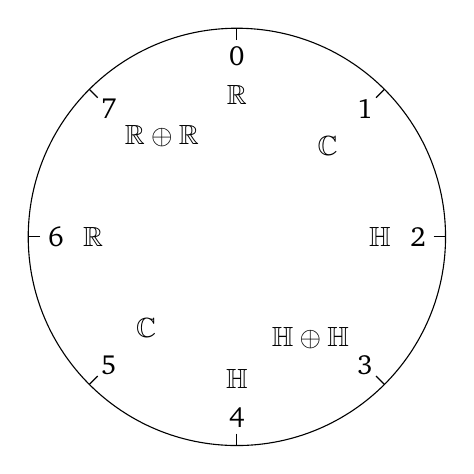
\begin{tikzpicture}
    \draw (0,0) circle[radius=2.65cm];
    \node[label=below:{$\mathbb{R}$}] at (90:2.3) {0};
    \node[label=below left:{$\mathbb{C}$}] at (45:2.3) {1};
    \node[label=left:{$\mathbb{H}$}] at (0:2.3) {2};
    \node[label={[label distance=-2mm]above left:{$\mathbb{H}\oplus\mathbb{H}$}}] at (-45:2.3) {3};
    \node[label=above:{$\mathbb{H}$}] at (-90:2.3) {4};
    \node[label=above right:{$\mathbb{C}$}] at (-135:2.3) {5};
    \node[label=right:{$\mathbb{R}$}] at (180:2.3) {6};
    \node[label={[label distance=-2mm]below right:{$\mathbb{R}\oplus\mathbb{R}$}}] at (135:2.3) {7};
    \foreach \a in {0,45,90,135,180,-135,-90,-45}
      \draw (\a:2.5) to (\a:2.65);
  \end{tikzpicture}
\] As I explained in \protect\hyperlink{week105}{``Week 105''}, this
clock easily lets you remember the real Clifford algebras in every
dimension and signature of spacetime. Bott periodicity explains why it
loops around after 8 hours. The spinorial chessboard presents the same
information in the form of an \(8\times 8\) grid. I won't draw it here,
but it's a picture of the Clifford algebras with \(p\) roots of \(-1\)
and \(q\) roots of \(1\) for \(p,q =0,1,2,3,4,5,6,7\). The black squares
correspond to cases that admit chiral spinors; the red ones correspond
to cases that don't. Black is when \(p+q\) is even; red is when it's
odd.

By the way, I have a little question: why does the above clock have a
reflection symmetry along the line joining \(\mathbb{R}+\mathbb{R}\) and
\(\mathbb{H}+\mathbb{H}\)?

Later, by coincidence, when I was in the library I discovered that
Chevalley's work on spinors has been reprinted:

\begin{enumerate}
\def\labelenumi{\arabic{enumi})}
\setcounter{enumi}{14}
\tightlist
\item
  Claude Chevalley, \emph{The Algebraic Theory of Spinors}, Springer,
  Berlin, 1991.
\end{enumerate}

It has a lot of neat stuff on ``pure spinors'', which are closely
related to the ``simple bivectors'' that describe 2-planes in
\(n\)-space. The latter play an important role in spin foam models of
quantum gravity, so I bet pure spinors will too.

Here's another fundamental text, which really helped get the whole
subject going:

\begin{enumerate}
\def\labelenumi{\arabic{enumi})}
\setcounter{enumi}{15}
\tightlist
\item
  Eli Cartan, \emph{The Theory of Spinors}, Dover Press, 1966.
\end{enumerate}

While I'm at it, I should mention this book by the infamous Pertti
Lounesto, which is also good:

\begin{enumerate}
\def\labelenumi{\arabic{enumi})}
\setcounter{enumi}{16}
\tightlist
\item
  Pertti Lounesto, \emph{Clifford Algebras and Spinors}, Cambridge U.
  Press, Cambridge, 1997.
\end{enumerate}

I also saw this book at a book fair:

\begin{enumerate}
\def\labelenumi{\arabic{enumi})}
\setcounter{enumi}{17}
\tightlist
\item
  Dominic Joyce, \emph{Compact Manifolds with Special Holonomy}, Oxford
  U. Press, Oxford, 2000.
\end{enumerate}

There's some incredible stuff here about 7-dimensional Riemannian
manifolds whose holonomy groups lie in the exceptional Lie group
\(\mathrm{G}_2\). I bet this stuff is gonna be important in string
theory someday --- if it isn't already. After all, \(\mathrm{G}_2\) is
the automorphism group of the octonions, and it has a 7-dimensional
irreducible representation on the imaginary octonions; as explained in
\protect\hyperlink{week104}{``Week 104''} by Robert Helling, the
octonions are secretly what let you write down the superstring
Lagrangian in 10d spacetime.

\begin{center}\rule{0.5\linewidth}{0.5pt}\end{center}

Footnote:

Andrzej Trautman answered my question about reflection symmetry in the
Clifford algebra clock by noting that
\[\mathrm{Cliff}(p,q) \otimes \mathbb{R}(2) = \mathrm{Cliff}(q+2,p)\]
where \(\mathbb{R}(2)\) is the algebra of \(2\times2\) real matrices. A
proof of this (actually well-known) fact appears in (7.8b) of his book.

In response to my list of most-cited papers, Aaron Bergman suggested the
following 261-page review article on the AdS-CFT correspondence:

\begin{enumerate}
\def\labelenumi{\arabic{enumi})}
\setcounter{enumi}{18}
\tightlist
\item
  O. Aharony, S. S. Gubser, J. Maldacena, H. Ooguri and Y. Oz, ``Large
  \(N\) field theories, string theory and gravity'', \emph{Phys. Rept.}
  \textbf{323} (2000) 183--386, preprint available as
  \href{https://arxiv.org/abs/hep-th/9905111}{\texttt{hep-th/9905111}}.
\end{enumerate}

For a similarly enormous review article on D-branes, try:

\begin{enumerate}
\def\labelenumi{\arabic{enumi})}
\setcounter{enumi}{19}
\tightlist
\item
  Clifford V. Johnson, ``D-brane primer'', preprint available as
  \href{https://arxiv.org/abs/hep-th/0007170}{\texttt{hep-th/0007170}}.
\end{enumerate}

Finally, it turns out that manifolds with \(\mathrm{G}_2\) holonomy
\emph{are} important in superstring theory, where they go by the name of
``Joyce manifolds''. Here are some places to read about them:

\begin{enumerate}
\def\labelenumi{\arabic{enumi})}
\setcounter{enumi}{20}
\item
  G. Papadopoulos and P. K. Townsend, ``Compactification of \(D=11\)
  supergravity on spaces of exceptional holonomy'', preprint available
  as
  \href{https://arxiv.org/abs/hep-th/9506150}{\texttt{hep-th/9506150}}.
\item
  B. S. Acharya, ``\(N=1\) heterotic-supergravity duality and Joyce
  manifolds'', preprint available as
  \href{https://arxiv.org/abs/hep-th/9508046}{\texttt{hep-th/9508046}}.

  ``\(N=1\) heterotic/M-theory duality and Joyce manifolds'', preprint
  available as
  \href{https://arxiv.org/abs/hep-th/9603033}{\texttt{hep-th/9603033}}.

  ``\(N=1\) M-theory-heterotic duality in three dimensions and Joyce
  manifolds'', preprint available as
  \href{https://arxiv.org/abs/hep-th/9604133}{\texttt{hep-th/9604133}}.

  ``Dirichlet Joyce manifolds, discrete torsion and duality'', preprint
  available as
  \href{https://arxiv.org/abs/hep-th/9611036}{\texttt{hep-th/9611036}}.

  ``M theory, Joyce orbifolds and super Yang-Mills'', preprint available
  as
  \href{https://arxiv.org/abs/hep-th/9812205}{\texttt{hep-th/9812205}}.
\item
  Chien-Hao Liu, ``On the global structure of some natural fibrations of
  Joyce manifolds'', preprint available as
  \href{https://arxiv.org/abs/hep-th/9809007}{\texttt{hep-th/9809007}}.
\end{enumerate}

I learned this thanks to Allen Knutson and Paul Schocklee. Paul also had
the following interesting comments:

\begin{quote}
John Baez wrote:
\end{quote}

\begin{quote}
\begin{quote}
There's some incredible stuff here about 7-dimensional Riemannian
manifolds whose holonomy groups lie in the exceptional Lie group
\(\mathrm{G}_2\).\\
I bet this stuff is gonna be important in string theory someday --- if
it isn't already.
\end{quote}
\end{quote}

\begin{quote}
They are important!
\end{quote}

\begin{quote}
If you want to directly compactify 11-dimensional supergravity/M-theory
to a theory with \(N=1\) supersymmetry in 4 dimensions, which is what
people like for phenomenological reasons, you need a 7-dimensional
manifold of \(\mathrm{G}_2\) holonomy (just as you need manifolds of
\(\mathrm{SU}(3)\) holonomy, i.e. Calabi-Yau manifolds, in six
dimensions). I have seen these referred to as ``Joyce manifolds,'' after
Dominic Joyce, who constructed several examples of such spaces. (I
didn't know there was so much known about them. I'll have to check out
the above book; I see that our library in Iceland has a copy.)
\end{quote}

\begin{quote}
Unfortunately, these models are afflicted by the usual problem of 11-d
SUGRA compactifications, which is that they are non-chiral, so these
days people seem to be concentrating more on Horava-Witten
compactifications, with M-theory on \(S^1/\mathbb{Z}_2\) times a
Calabi-Yau, or on an orbifold.
\end{quote}

\begin{quote}
If you're interested, you might want to check out Papadopoulos and
Townsend, ``Compactification of D=11 supergravity on spaces of
exceptional holonomy,'' https://arxiv.org/abs/hep-th/9506150.
\end{quote}

\begin{quote}
-- Paul Shocklee Graduate Student, Department of Physics, Princeton
University Researcher, Science Institute, Dunhaga 3, 107 Reykjavk,
Iceland Phone: +354-525-4429
\end{quote}

\begin{center}\rule{0.5\linewidth}{0.5pt}\end{center}
\hypertarget{week155}{%
\section{DATE}\label{week155}}

It's a hot summer day here in Riverside, so I just want to have fun.
Break out the Klein bottles and Platonic solids!

I still remember the day as a kid when I first made a Möbius strip, and
saw how it didn't fall apart when cut in half. I could see it, but I
couldn't quite grok it. I was fascinated --- and more than a little
annoyed when it turned out my dad already knew about it.

I don't remember exactly when I first saw a Klein bottle, but I loved it
at first sight:

\begin{verbatim}
            A mathematician named Klein
            Thought the Möbius strip was divine.
            Said he: "If you glue 
            The edges of two
            You'll get a weird bottle like mine!"
\end{verbatim}

Recently, when I was trying to explain some stuff about Klein bottles to
my friend Oz on \texttt{sci.physics.research}, I bumped into the website
of a company that sells the things --- Acme Klein Bottles. I couldn't
resist mentioning to the world at large that I'd dearly like one. And lo
and behold, a regular reader of This Week's Finds took me up on this:
Timothy J. Kordas. After a few weeks, a handcrafted glass Klein bottle
arrived via United Parcel Service. It's great! --- it sits on my desk
now, gleaming contentedly. I think everybody should have one. You can
even buy them sliced in half, exhibiting the Möbius strip quite clearly:

\begin{enumerate}
\def\labelenumi{\arabic{enumi})}
\tightlist
\item
  Acme Klein bottles sliced in half,
  \texttt{http://www.kleinbottle.com/sliced\_klein\_bottles.htm}
\end{enumerate}

Meanwhile, I've been thinking about the Platonic solids lately, and also
their generalizations to higher dimensions --- the so-called ``regular
polytopes''. To really learn about regular polytopes, you have to go to
the source: the king of geometry, Harold Scott Macdonald Coxeter. But
for some reason I didn't get around to reading his books until just
recently:

\begin{enumerate}
\def\labelenumi{\arabic{enumi})}
\setcounter{enumi}{1}
\item
  H. S. M. Coxeter, \emph{Regular Polytopes}, 3rd edition, Dover, New
  York, 1973.

  \emph{Regular Complex Polytopes}, 2nd edition, Cambridge U. Press,
  Cambridge, 1991.
\end{enumerate}

Now my head is full of neat facts about regular polytopes, so I want to
rattle some off before I forget!

Let's start in 3 dimensions. I assume you're friends with the
tetrahedron, cube, octahedron, dodecahedron and icosahedron. But you
might not know all the nice relationships between them!

For example, there's a nice way to fit a tetrahedron snugly into a cube:
if you take every other vertex of the cube, you get the vertices of a
tetrahedron. And of course I mean a \emph{regular} tetrahedron --- I'm
not interested in any other kind, here. There are two ways to do this,
and if you put both these tetrahedra inside the cube, they combine to
form a star-shaped solid called the ``stella octangula''. This was
discovered and given its name by Kepler, who was really fond of this
sort of thing.

Here's a picture:

\begin{enumerate}
\def\labelenumi{\arabic{enumi})}
\setcounter{enumi}{2}
\tightlist
\item
  Eric Weisstein, stella octangula,
  \texttt{http://mathworld.wolfram.com/StellaOctangula.html}
\end{enumerate}

You can rotate it by grabbing it with your mouse!

Similarly, there is a nice way to fit a cube in a dodecahedron. The
dodecahedron has 20 vertices, and we can use 8 of these as the vertices
of a cube. This becomes obvious once we realize that these points are
the vertices of a dodecahedron: \[
  \begin{gathered}
    (\pm 1/G, \pm G, 0),
  \\(\pm G, 0, \pm 1/G),
  \\(0, \pm 1/G, \pm G)
  \\(\pm1, \pm1, \pm1).
  \end{gathered}
\] where \(G = (\sqrt{5} + 1)/2\) is the golden ratio and we get to pick
each of the plus or minus signs independently. The points
\((\pm1, \pm1, \pm1)\) form the vertices of a cube.

By rotating the whole picture, we get some other ways of putting a cube
in a dodecahedron: 5 in all. Any rotation of the dodecahedron permutes
these 5 cubes, and we get all even permutations of the cubes this way:
this is one nice way to prove that the rotational symmetry group of the
dodecahedron is \(A_5\) (the group of even permutations of 5 things).

If we put all 5 cubes inside the dodecahedron, we get a fancy shape that
would make a marvelous Christmas tree decoration --- I don't know what
it's called, but you can see a picture of it in Coxeter's ``Regular
Polytopes'', and also here:

\begin{enumerate}
\def\labelenumi{\arabic{enumi})}
\setcounter{enumi}{3}
\tightlist
\item
  Eric Weisstein, cube 5-compound,
  \texttt{http://mathworld.wolfram.com/Cube5-Compound.html}
\end{enumerate}

Now let's combine these two tricks. If we put a tetrahedron in a cube,
and then put the cube in a dodecahedron, we get a way of fitting the
tetrahedron snugly into the dodecahedron! If we choose one way of doing
this and then rotate the picture to get other ways, we get 5 tetrahedra
in the dodecahedron. Putting these all together gives a scary-looking
shape:

\begin{enumerate}
\def\labelenumi{\arabic{enumi})}
\setcounter{enumi}{4}
\tightlist
\item
  Eric Weisstein, tetrahedron 5-compound,
  \texttt{http://mathworld.wolfram.com/Tetrahedron5-Compound.html}
\end{enumerate}

but the coolest thing about this shape is that it has an inherent
handedness --- like a sugar molecule, it comes in ``levo'' and
``dextro'' forms! If we reflect it, we get 5 \emph{other} ways to put a
tetrahedron into a dodecahedron, for a total of 10. All of these
tetrahedra taken together form a mirror-symmetric shape:

\begin{enumerate}
\def\labelenumi{\arabic{enumi})}
\setcounter{enumi}{5}
\tightlist
\item
  Eric Weisstein, tetrahedron 10-compound,
  \texttt{http://mathworld.wolfram.com/Tetrahedron10-Compound.html}
\end{enumerate}

Okay. So far we've related the tetrahedron, the cube and the
dodecahedron. What about the other two Platonic solids: the octahedron
and icosahedron? Well, from the point of view of \emph{symmetry groups}
these guys are redundant. The octahedron is dual to the cube, so it has
the same rotational symmmetry group. Similarly, the icosahedron is dual
to the dodecahedron and has the same symmetry group.

From the group-theoretic viewpoint, here's what's really going on. Our
trick for fitting the tetrahedron in the cube lets us turn any symmetry
of the tetrahedron into a symmetry of the cube. The rotational symmetry
group of the tetrahedron is \(A_4\) --- that is, all even permutations
of the 4 vertices. The symmetry group of the cube is \(S_4\) --- that
is, all permutations of the 4 lines connecting opposite vertices. So
what we've got is a trick for making \(A_4\) into a subgroup of \(S_4\).

(This immediately leads to a little puzzle. There's an \emph{obvious}
way to find \(A_4\) as a subgroup of \(S_4\), since even permutations
are a special case of permutations. So: does the above trick give this
obvious way, or some other way?)

Anyway, it's also true that any way of fitting the tetrahedron in the
dodecahedron lets us turn any symmetry of the tetrahedron into a
symmetry of the dodecahedron. So we've also got a trick for making
\(A_4\) into a subgroup of \(A_5\).

(You might also think that our trick for fitting the cube in the
dodecahedron gives a way to turn any symmetry of the cube into a
symmetry of the dodecahedron. I thought this for a while, but it's not
true! For starters, if it \emph{were} true, we'd get a trick for making
\(S_4\) into a subgroup of \(A_5\) --- which is impossible, since the
order of the group \(S_4\) doesn't divide that of \(A_5\). And the
problem turns out to be this: a 90 degree rotation of the cube does not
correspond to a symmetry of the dodecahedron.)

Playing with this stuff would be a nice way to start learning group
theory --- but even if you already know group theory, it's sort of fun.
For more along these lines, try:

\begin{enumerate}
\def\labelenumi{\arabic{enumi})}
\setcounter{enumi}{6}
\tightlist
\item
  John Baez, Some thoughts on the number 6,
  \texttt{http://math.ucr.edu/home/baez/six.html}
\end{enumerate}

Check out the new link to Greg Egan's website illustrating some of the
concepts!

Now, despite their redundancy from the group-theoretic viewpoint, it's
unfair to leave the octahedron and icosahedron out in the cold. These
guys should be related somehow. After all, the octahedron has 12 edges,
while the icosahedron has 12 vertices. Is there any way we can exploit
this fact?

Yes! The octahedron is the only Platonic solid whose faces can be
colored black and white so that no two faces of the same color share an
edge. So go ahead: grab a regular octahedron and color it like that.
Next, pick an edge and start marching along it with the white face to
your left and the black face to your right. Go \(1/G\)th of the way,
where \(G\) is the golden ratio again, and mark this point with a dot.
Now do this for all the edges. You'll get 12 dots --- and these dots
form the vertices of a regular icosahedron!

Next, let's take a quick tour of the 4th dimension. This is the most
exciting dimension for regular polytopes. In all higher dimensions there
are only three --- analogues of the tetrahedron, cube and octahedron.
But in 4 dimensions, there are six.

I won't describe these systematically here. For that you should read
Coxeter's books, or if you're in a rush, my webpage:

\begin{enumerate}
\def\labelenumi{\arabic{enumi})}
\setcounter{enumi}{7}
\tightlist
\item
  John Baez, ``Platonic solids in all dimensions'',
  \texttt{http://math.ucr.edu/home/baez/platonic.html}
\end{enumerate}

Instead, I'll just talk about a cool relationship between my two
favorite 4d regular polytopes: the 24-cell and the 600-cell.

First let me set the stage, by reminding you what these look like. A
24-cell looks like this:

\begin{enumerate}
\def\labelenumi{\arabic{enumi})}
\setcounter{enumi}{8}
\tightlist
\item
  Eric Weisstein, 24-cell,
  \texttt{http://mathworld.wolfram.com/24-Cell.html}
\end{enumerate}

To visualize it on your own, first imagine a hypercube with vertices
\[(\pm1,\pm1,\pm1,\pm1)\] Then imagine the 4-dimensional analogue of an
octahedron --- usually called a ``cross-polytope'' --- with vertices \[
  \begin{gathered}
    (\pm2,0,0,0),
  \\(0,\pm2,0,0),
  \\(0,0,\pm2,0),
  \\(0,0,0,\pm2).
  \end{gathered}
\] The hypercube has 16 vertices and the cross-polytope has 8. I've set
things up so that all 24 of these points have the same distance from the
origin. These are the vertices of the 24-cell!

But the 24-cell does not get its name from having 24 vertices. It gets
its name from having 24 faces! It has 24 octahedral faces, 96 triangles,
96 edges and 24 vertices. The symmetry here comes from the fact that the
24-cell is self-dual --- which comes from the fact that we've built it
from two polytopes that are dual to each other: the hypercube and the
cross-polytope.

What would happen if we had tried this trick in 3 dimensions? Let's see!
Take a cube and take an octahedron. Center them both at the origin, line
them up nicely, and rescale them so all their vertices are the same
distance from the origin: say \[(\pm1,\pm1,\pm1)\] and \[
  \begin{gathered}
    (\pm\sqrt{3},0,0),
  \\(0,\pm\sqrt{3},0),
  \\(0,0,\pm\sqrt{3}).
  \end{gathered}
\] We get a shape with \(8 + 6 = 14\) vertices. But it's not a Platonic
solid --- it's a rhombic dodecahedron! Apparently this too was first
discovered by Kepler. You can view one, and even rotate it by hand, at
this webpage:

\begin{enumerate}
\def\labelenumi{\arabic{enumi})}
\setcounter{enumi}{9}
\tightlist
\item
  Kevin Brown, Kepler's rhombic dodecahedron,
  \texttt{http://www.seanet.com/\textasciitilde{}ksbrown/coinc2.htm}
\end{enumerate}

Here's another way to think about this stuff. Take two cubes, equal in
size. Chop one up into 6 pyramids, each having one face of the cube as
its base, and each having the cube's center as its apex. Now take these
6 pyramids and glue their bases onto the faces of the other cube. What
do you get? A rhombic dodecahedron! If can't visualize this, go here:

\begin{enumerate}
\def\labelenumi{\arabic{enumi})}
\setcounter{enumi}{10}
\tightlist
\item
  Mark Newbold's rhombic dodecahedron page,
  \texttt{http://dogfeathers.com/mark/rhdodec.html}
\end{enumerate}

Now do the same thing in 4 dimensions. Take two hypercubes, equal in
size. Chop one up into 8 ``hyperpyramids'', each having one face of the
hypercube as its base, and each having the hypercube's center as its
apex. Now take these hyperpyramids and glue their bases onto the faces
of the other hypercube. What do you get? The 24-cell!

(Of course, one can play this game in any dimension, but it works best
in dimension 4. I could explain why, but it's probably better to figure
it out yourself.)

Okay. Now for the 600-cell. This one is harder: it has 600 tetrahedral
faces, 1200 triangles, 720 edges, and 120 vertices. When Buckminster
Fuller died and went to heaven, he probably took up residence in one of
these. It looks like this:

\begin{enumerate}
\def\labelenumi{\arabic{enumi})}
\setcounter{enumi}{11}
\tightlist
\item
  Eric Weisstein, 600-cell,
  \texttt{http://mathworld.wolfram.com/600-Cell.html}
\end{enumerate}

Here's how you build one. Start with 600 regular tetrahedra. Take 20 of
them and glue them together so they all meet at one vertex and the
outside looks just like an icosahedron. Of course you can't do this in
flat 3-dimensional space: there's ``wiggle room'' left over when you
try! So you have to bend the whole setup a little bit into the 4th
dimension, like a piece of a 4d geodesic dome. Then keep adding more
tetrahedra, always making sure that 20 meet at each vertex in an
icosahedral pattern. By the time you've used up all of them, your
600-cell will be complete --- a nice rigid structure.

Of course, if you're a mathematician, there are other more elegant ways
to build your 600-cell. For example: start with an icosahedron. Its
rotational symmetry group is a 60-element subgroup of
\(\mathrm{SO}(3)\). Using the double cover
\(\mathrm{SU}(2) \to \mathrm{SO}(3)\) lift this to a 120-element
subgroup of \(\mathrm{SU}(2)\). But \(\mathrm{SU}(2)\) is isomorphic to
the unit quaternions, so we get 120 points on the unit sphere in 4
dimensions. These are the vertices of the 600-cell!

In fact we can construct the 24-cell in the same way, as I explained in
\href{week91.html}{week91}. Here we start with the tetrahedron, whose
rotational symmetry group is a 12-element subgroup of
\(\mathrm{SO}(3)\), and we get 24 points on the unit sphere in 4
dimensions, which are the vertices of the 24-cell.

But if you really want to show off, you can build a 600-cell starting
from a 24-cell! Here's how. It's a bit like the trick where we started
with an octahedron, systematically marked a point \(1/G\)th of the way
along each edge, and got the vertices of an icosahedron. But it's
fancier.

Start with the 24-cell. Take any edge, start walking down it, and when
you've gone \(1/G\)th of the way, mark that point with a dot. Of course
these instructions are ambiguous, since I didn't tell you which end of
the edge to start at! I could tell you, but I won't --- I'll just say
that if you do it \emph{the right way}, you'll get 96 dots which are the
vertices of a marvelous polytope in 4 dimensions. It's not a regular
polytope, but it's ``semiregular'': it has 24 regular icosahedra and 120
regular tetrahedra as faces. Coxeter calls it \(s\{3,4,3\}\), but it
really deserves a more glamorous name.

Now as we've seen, in 4 dimensions there is a way to glue 20 tetrahedra
together in an icosahedral pattern. You can picture this as a squat
pyramid-shaped gadget with a regular icosahedron as base and 20
tetrahedral faces all meeting at the apex.

So: glue one of these pyramid-shaped gadgets onto each of the 24
icosahedral faces of our \(s\{3,4,3\}\). We get a polytope which has
\(20\times 24\) new tetrahedral faces in addition to the 120 original
tetrahedral faces of our \(s\{3,4,3\}\), for a total of 600. Voila ---
it's the 600-cell!

For the proof that all this works as advertised, read Coxeter's
``Regular Polytopes''. Note that it's really easier to work backwards:
start with the 600-cell, then truncate it to get \(s\{3,4,3\}\).

Okay, now for one last trick. I actually thought of this myself ---
though I can't believe it's new. It gives a way to see the vertices of
the 24-cell as a subset of the vertices of the 600-cell.

As I already said, the rotational symmetry group of the tetrahedron has
a ``double cover'' consisting of 24 unit quaternions, which happen to be
precisely the vertices of the 24-cell.

Similarly, the rotational symmetry group of the dodecahedron has a
``double cover'' consisting of 120 unit quaternions, which happen to be
precisely the vertices of the 600-cell.

Any way of fitting the tetrahedron snugly into the dodecahedron
therefore gives a way of making the vertices of the 24-cell into a
subset of the vertices of the 600-cell!

Now, we've already seen 10 ways of snugly fitting the tetrahedron into
the dodecahedron: 5 which make the ``levo'' form of that scary-looking
shape, and 5 which make the ``dextro'' form. The first 5 give 5
different ways of stuffing the 24-cell into the 600-cell. But the second
5 give nothing new.

So this trick actually gives us 5 ways of making the vertices of the
24-cell into a subset of the vertices of the 600-cell. And all these
ways have one vertex in common, corresponding to the element 1 of the
unit quaternions.

Okay, that's it for this week. No serious stuff this time. I just want
to mention that in addition to the above websites, there are a lot that
show polyhedra in a way that requires red-blue 3d glasses or a VRML
plugin. Since I don't have either of these, and you might not either,
I've avoided links to those pages. By the way, VRML stands for ``virtual
reality modelling language'', but it's really just a language for
delivering interactive 3d objects over the web. If you can handle VRML,
you can probably have a lot of fun here:

\begin{enumerate}
\def\labelenumi{\arabic{enumi})}
\setcounter{enumi}{12}
\tightlist
\item
  George W. Hart's Pavilion of Polyhedrality,
  \texttt{http://www.georgehart.com/pavilion.html}
\end{enumerate}

If you don't, you can still enjoy the annotated bibliography and links
to other websites. You can also get a lot out of Vladimir Bulatov's
collection of polyhedra without VRML, but again, it's better if you have
it:

\begin{enumerate}
\def\labelenumi{\arabic{enumi})}
\setcounter{enumi}{13}
\tightlist
\item
  Victor Bulatov's Polyhedra Collection,
  \texttt{http://www.physics.orst.edu/\textasciitilde{}bulatov/polyhedra/index.html}
\end{enumerate}

Finally, if you're good at crossing your eyes, you can see some
4-dimensional polytopes at this website, which also has a lot of cool
information on how the 4d regular polytopes are related to other
branches of math:

\begin{enumerate}
\def\labelenumi{\arabic{enumi})}
\setcounter{enumi}{14}
\tightlist
\item
  Tony Smith, 24-cell animation, 120-cell, 600-cell,
  \texttt{http://www.innerx.net/personal/tsmith/24anime.html}
\end{enumerate}

I thank Jim Heckman and Noam Elkies for helping me fix some errors in
the original version of this article.

\begin{center}\rule{0.5\linewidth}{0.5pt}\end{center}
\hypertarget{week156}{%
\section{DATE}\label{week156}}

This week I want to catch you up on some of the experiments that have
been going on lately. Mathematical physics is no fun without some
experiments to think about now and then. So here's some news about black
holes, superfluid hydrogen, T violation, the \(\tau\) neutrino, and the
Higgs boson.

I like black holes because they are a nice example of what general
relativity can do. Once upon a time they seemed very exotic, but now it
seems they're common. In particular, there appear to be black holes with
masses between a million and several billion times that of the Sun at
the centers of all galaxies with a ``bulge''. This includes galaxies
like the Milky Way, which has a central bulge in addition to a flat
spinning disk, and also elliptical galaxies, which consist solely of a
bulge. Many of these supermassive black holes emit lots of X-rays as
they swallow hapless stars. As I mentioned in
\href{week144.html}{week144}, the X-ray telescope Chandra has seen
evidence for about 70 million of these black holes!

Recently, two teams of researchers have found that the mass of these
central black holes is correlated very closely to the dispersion of
stellar velocities in the galaxy:

\begin{enumerate}
\def\labelenumi{\arabic{enumi})}
\item
  John Kormendy, ``Monsters at the heart of galaxy formation'',
  \emph{Science} \textbf{289} (2000), 1484--1485. Available online at
  \texttt{http://www.sciencemag.org/cgi/content/full/289/5484/1484}
\item
  Laura Ferrarese and David Merritt, ``A fundamental relation between
  supermassive black holes and their host galaxies'', \emph{Astrophys.
  J. Lett.} \textbf{539}, (2000) L9, preprint available as
  \href{https://arxiv.org/abs/astro-ph/0006053}{\texttt{astro-ph/0006053}}.
\item
  Karl Gebhardt et al, ``A relationship between nuclear black hole mass
  and galaxy velocity dispersion'', \emph{Astrophys. J. Lett.}
  \textbf{539}, (2000) L13, preprint available as
  \href{https://arxiv.org/abs/astro-ph/0006289}{\texttt{astro-ph/0006289}}.
\end{enumerate}

Tight correlations are a bit rare in astrophysics, so they tend to be
important when they exist. If you look at a graph you'll see how nice
this one is:

\begin{enumerate}
\def\labelenumi{\arabic{enumi})}
\setcounter{enumi}{3}
\tightlist
\item
  Supermassive Black Hole Group, ``Theory of black holes and galaxies'',
  \texttt{http://www.physics.rutgers.edu/\textasciitilde{}merritt/theory.htm}
\end{enumerate}

Ferrarese and Merrit estimate that the black hole mass grows as roughly
the 4.8th power of the stellar velocity dispersion, which they define as
the standard deviation of the radial component of the velocities of
stars in the galaxy.

But what does this correlation \emph{mean}? Astrophysicists are still
arguing about that. But at the very least, it suggests an intimate
relation between supermassive black holes and the process of galaxy
formation.

Part of the puzzle is that nobody knows how these supermassive black
holes formed. You see, until very recently, all we've ever seen are
small black holes formed by the collapse of a single star (between 3 and
20 solar masses), and these supermassive ones at the centers of
galaxies. But last year, people started seeing middle- sized ones!
Colbert and Mushotzky found black holes between 100 and 10,000 solar
masses in about half of 30 nearby spiral and elliptical galaxies that
they examined:

\begin{enumerate}
\def\labelenumi{\arabic{enumi})}
\setcounter{enumi}{4}
\item
  Ed Colbert's homepage,
  \texttt{http://www.pha.jhu.edu/\textasciitilde{}colbert/}

  E. J. M. Colbert and R. F. Mushotzky, ``The nature of accreting black
  holes in nearby galaxy nuclei'', preprint available as
  \href{https://arxiv.org/abs/astro-ph/9901023}{\texttt{astro-ph/9901023}}.
\end{enumerate}

Ptak and Griffiths found a black hole of over 460 solar masses in an
irregular galaxy called M82:

\begin{enumerate}
\def\labelenumi{\arabic{enumi})}
\setcounter{enumi}{5}
\tightlist
\item
  A. Ptak, R. Griffiths, ``Hard X-ray variability in M82: evidence for a
  nascent AGN?'', preprint available as
  \href{https://arxiv.org/abs/astro-ph/9903372}{\texttt{astro-ph/9903372}}.
\end{enumerate}

This is a ``starburst galaxy'', meaning that it's full of supernovae
going off like a big firework display. When a star dies in a supernova
explosion, that's when a neutron star or black hole is formed --- so it
seems likely that this black hole in M82 was formed by the merger of
several such black holes. Could we be seeing the gradual formation of a
supermassive black hole?

Maybe someday we'll understand the complete ecology of black holes. I
can't help but feel there's some important role they play which we don't
understand yet. (For one theory about this, see the end of
\href{week33.html}{week33}.)

Now: you've all heard how helium-4 becomes a superfluid below 2.18
kelvin and helium-3 does it below 2.4 millikelvin. But what about
superfluid hydrogen? Unlike helium, hydrogen is not a snobbish loner:
it's a friendly, sticky molecule. So usually it solidifies before it
gets cold enough to go superfluid! But in 1997, some folks at the
University of Illinois noticed a possible loophole: films of liquid
hydrogen about one molecule thick on a silver substrate should form a 2d
superfluid at a temperature of 1.2 kelvin. Here's a picture of a
computer simulation:

\begin{enumerate}
\def\labelenumi{\arabic{enumi})}
\setcounter{enumi}{6}
\tightlist
\item
  David Ceperley et al, ``Prospective superfluid molecular hydrogen'',
  \texttt{http://www.aip.org/physnews/graphics/html/h2.htm}
\end{enumerate}

Since then, other people have cooked up other schemes.

Now it seems people have actually made the stuff. Tiny amounts of it!
The way they do it is to take superfluid helium and put in a bit of
carbonyl sulfide (OCS) and hydrogen. About 14 to 16 hydrogen molecules
stick to the carbonyl sulfide molecule, and when the temperature drops
to .15 kelvin, these molecules form a superfluid. The hard part is
checking experimentally that this really happens --- and even
\emph{defining} what it means for a cluster of so few molecules to be a
superfluid. I can't explain the details; for that you'll have to read
the paper:

\begin{enumerate}
\def\labelenumi{\arabic{enumi})}
\setcounter{enumi}{7}
\tightlist
\item
  Slava Grebenev, Boris Sartakov, J. Peter Toennies, and Andrei F.
  Vilesov, ``Evidence for superfluidity in para-hydrogen clusters inside
  helium-4 droplets at 0.15 Kelvin'', \emph{Science} \textbf{5484}
  (2000), 1532--1535, available online at
  \texttt{http://www.sciencemag.org/cgi/content/abstract/289/5484/1532}
\end{enumerate}

Here ``para-hydrogen'' refers to a molecule of hydrogen where the spins
on the two nuclei are anti-parallel --- as opposed to
``ortho-hydrogen'', where they're lined up. The two states have
different properties and this matters a lot in delicate situations like
these.

Next: T violation. Once people thought the laws of physics were
symmetrical under exchanging either particles with their antiparticles,
left with right, or future with past. These three symmetries are called
C (for ``charge conjugation''), P (for ``parity'') and T (for ``time
reversal''). The weak interaction is now believed to violate all of
these.

Very briefly, the story goes like this: Yang and Lee won the Nobel prize
for helping discover P violation in the \(\beta\) decay of radioactive
cobalt back in 1956, though in retrospect it was only the sexism of the
Nobel committee that prevented Wu from sharing this prize --- she did
the actual experiment. In \(\beta\) decay, a neutron turns into a
proton, an electron and an electron anti-neutrino via the weak
interaction. Since the electron anti-neutrino only comes in a
right-handed form, this process violates P symmetry.

Cronin and Fitch won the Nobel prize for discovering in 1964 that
neutral kaons decay in a way that violates CP symmetry --- i.e., the
symmetry where you switch particles with their antiparticles \emph{and}
switch left with right. I believe that neutral kaons are still the only
system where CP violation has been seen.

Now there's something called the CPT theorem which says that various
reasonable axioms for a quantum field theory imply symmetry under the
\emph{combination} of C, P and T. For the math of this, the obvious
place to go is this classic text on axiomatic quantum field theory:

\begin{enumerate}
\def\labelenumi{\arabic{enumi})}
\setcounter{enumi}{8}
\tightlist
\item
  R. F. Streater and A. S. Wightman, \emph{PCT, Spin and Statistics, and
  All That}, Addison-Wesley, Reading, Massachusetts, 1989.
\end{enumerate}

In case you're worried, PCT is the same thing as CPT. I like this book a
lot. The only thing I dislike is how it unleashed a flood of physics
papers whose titles end with ``and all that''. For example:

\begin{itemize}
\tightlist
\item
  ``CFT, BCFT, ADE and all that''
\item
  ``Quantum cohomology and all that''
\item
  ``String theory, supersymmetry, unification, and all that''
\item
  ``Anti-de Sitter space, branes, singletons, superconformal field
  theories and all that''
\item
  ``The modified Bargmann-Wigner formalism: longitudinal fields, parity
  and all that''
\item
  ``The Zamolodchikov C-Function, classical closed string field theory,
  the Duistermaat-Heckman theorem, the renormalization group, and all
  that''
\end{itemize}

Enough! Listen, guys: it was funny once, but now it's just lame. Stop
it!

But I digress. Where was I? Oh yeah: given the CPT theorem, from CP
violation we can conclude T violation. The future and the past are
slightly different --- but of all the known forces, only the weak force
notices the difference! This is bizarre and fascinating. But the way we
reached this conclusion was not completely satisfying, since we needed
to assume the usual axioms of quantum field theory to get the CPT
theorem. What if the axioms are wrong? It would be better to have more
\emph{direct} evidence of T violation, given how important this issue
is.

So in the late 1990s, people in the CPLEAR collaboration at CERN did
some precision experiments on neutral kaon decay, and found more direct
evidence of T violation!

\begin{enumerate}
\def\labelenumi{\arabic{enumi})}
\setcounter{enumi}{9}
\item
  CPLEAR homepage,
  \texttt{http://cplear.web.cern.ch/cplear/Welcome.html}
\item
  CPLEAR collaboration, ``First direct observation of time-reversal
  non-invariance in the neutral kaon system'', \emph{Phys. Lett.}
  \textbf{B 444} (1998) 43, available online with all other papers by
  this collaboration at
  \texttt{http://cplear.web.cern.ch/cplear/cplear\_pub.html}
\end{enumerate}

Now we can all sit back and rack our brains even harder about what T
violation really \emph{means}. So far, all we know is that it arises
from the darkest corner of the Standard Model: the Kobayashi-Maskawa
matrix. This is a matrix describing quarks' couplings to the Higgs. The
fact that it's not diagonal means that the ``flavor eigenstates'' of the
quarks - up and down, strange and charmed, bottom and top --- are not
the ``mass eigenstates''. Why does the Kobayashi-Maskawa matrix equal
what it equals? Why is it of a form that violates T symmetry? Nobody
knows.

Another nice confirmation of what we already believed was the recent
discovery of direct evidence for the \(\tau\) neutrino. If you don't
remember the particles in the Standard Model, try
\href{week119.html}{week119}: you'll see that it has 3 generations of
quarks (listed above) and 3 generations of leptons: the electron, muon
and \(\tau\) and their corresponding neutrinos. Of the leptons, the
\(\tau\) is the heaviest and thus hardest to produce. Tau neutrinos are
produced by the decay of \(\tau\) particles, but since it's hard to make
these particles and hard to catch neutrinos, until recently nobody had
ever done the clinching experiment: creating a beam of a \(\tau\)
neutrinos and letting it collide with some stuff to form \(\tau\)
particles again.

On July 21st, 2000, the DONUT collaboration at Fermilab announced that
they had successfully done this experiment:

\begin{enumerate}
\def\labelenumi{\arabic{enumi})}
\setcounter{enumi}{11}
\tightlist
\item
  Christina Hebert, ``Phyisicists find first direct evidence for
  \(\tau\) neutrino at Fermilab'',
  \texttt{http://www.fnal.gov/directorate/public\_affairs/story\_neutrino/p1.html}
\end{enumerate}

In case you're wondering, ``DONUT'' stands for ``Direct Observation of
the Nu Tau'', where \(\nu_\tau\) is the standard abbrevation for
\(\tau\) neutrino.

In short, the final details of the Standard Model are all falling into
place just as expected --- except for the fact that neutrinos are doing
lots of weird stuff they shouldn't be doing! As I explained in
\href{week130.html}{week130}, neutrino physics is the big place for
surprises in particle physics these days. This is yet another reason why
it was good to directly observe the \(\tau\) neutrino.

And then, of course, there's the Higgs --- the final particle in the
Standard Model. As you've probably heard, we're getting awfully close to
seeing it --- or at least definitively \emph{not} seeing it. Right now
they're looking for it at LEP --- the big particle accelerator at CERN,
in Geneva. They're just about to shut LEP down, since it's done pretty
much all it can do, and they need to deactivate it to build an even more
powerful accelerator --- LHC, the Large Hadron Collider. But at the last
minute they decided to extend its life to November 2nd, 2000:

\begin{enumerate}
\def\labelenumi{\arabic{enumi})}
\setcounter{enumi}{12}
\tightlist
\item
  LEP shutdown postponed by one month,
  \texttt{http://press.web.cern.ch/Press/Releases00/PR08.00ELEPRundelay.html}
\end{enumerate}

They're going for broke, boosting its power to the utter max, so that
they can see hints of the Higgs as long as its mass is 114 GeV or so. In
fact they have already seen a couple of events that suggest a Higgs of
about this mass.

Whether or not LEP sees the Higgs the folks at the Tevatron at Fermilab
should see it when they start Run II in a while, as long as its mass
below 130 GeV. And if \emph{they} don't see it, folks at CERN should see
it with the LHC accelerator by around 2005, as long as its mass is below
180 GeV. A Higgs more massive than that would mean the Standard Model is
seriously screwed up, so at that point, even \emph{not} seeing the Higgs
would be an important discovery.

The folks getting ready to analyze the Run II data at the Tevatron are
doing so with a few theories in mind: the Standard Model, the minimal
supersymmetric extension of the Standard Model, and a
``next-to-minimal'' supersymmetric extension. This is a major project;
you can find lots of details here:

\begin{enumerate}
\def\labelenumi{\arabic{enumi})}
\setcounter{enumi}{13}
\tightlist
\item
  Higgs Working Group webpage,
  \texttt{http://fnth37.fnal.gov/higgs/higgs.html}
\end{enumerate}

That's basically it for this week. I just have a couple of questions
about CPT. A while back on sci.physics.research I emphasized a little
theorem that says: any self-dual irreducible unitary group
representation H must admit an antiunitary intertwiner
\(J\colon H \to H\) with either \(J^2 = 1\) or \(J^2 = -1\). In the
first case \(H\) comes from a real representation; in the second case it
comes from a quaternionic representation. For more details, try this:

\begin{enumerate}
\def\labelenumi{\arabic{enumi})}
\setcounter{enumi}{14}
\tightlist
\item
  John Baez, Symplectic, quaternionic, fermionic,
  \texttt{http://math.ucr.edu/home/baez/symplectic.html}
\end{enumerate}

Now, after I mentioned this, someone who goes by the name of ``squark''
suggested that the CPT operator for massive spin-\(1/2\) particles was
an antiunitary intertwiner with \((\mathrm{CPT})^2 = -1\). I'm not sure
this is true, but it's definitely antiunitary, so we have an intesting
question: which unitary irreducible representations of the Poincare
group are self-dual? Of these, which come from real representations and
which come from quaternionic ones? My hunch is that the bosonic (i.e.
integral-spin) reps are real and the fermionic (i.e.~half-integral-spin)
reps are quaternionic. And then the question is: is the operator \(J\)
just the the CPT operator? This would certainly shed some nice
mathematical light on the meaning of CPT symmetry.

By the way, This Week's Finds has a nice new feature, courtesy of
Laurent Bartholdi: now you can search all the old issues for a keyword
or phrase! This is very useful, at least for me. Check it out on my
website.

\begin{center}\rule{0.5\linewidth}{0.5pt}\end{center}

Footnotes:

Squark found in Volume 1 of Weinberg's ``Quantum Field Theory'' that the
CPT operator on the Hilbert space of a spin-\(j\) representation of the
Poincare group is an antiunitary operator with
\((\mathrm{CPT})^2 = -1^{2j}\). So indeed we do have
\((\mathrm{CPT})^2 = 1\) in the bosonic case, making these
representations real, and \((\mathrm{CPT})^2 = -1\) in the fermionic
case, making these representations quaternionic.

Allen Knutson points out that Streater and Wightman's title ``PCT, Spin
and Statistics, and All That'' was itself modelled after that of Sellar
and Yeatman's humorous history: ``1066 and all that; a memorable history
of England, comprising all the parts you can remember including one
hundred and three good things, five bad kings and two genuine dates.''

Martin Hardcastle wonders if Streater and Wightman were inspired by the
similarity of their names to those of Sellar and Yeatman!

\begin{center}\rule{0.5\linewidth}{0.5pt}\end{center}
\hypertarget{week157}{%
\section{DATE}\label{week157}}

I never write issues of This Week's Finds about topics that people
request. I only write about what I happen to be studying at a given
moment --- nothing else seems to work. But when my friend Minhyong Kim
asked me to do an issue on Young diagrams, I decided to break this rule
just once. Young diagrams are too cool to ignore.

Physics relies a lot on \emph{symmetry} to simplify problems, and there
are two kinds of diagrams that show up a lot in this context: Dynkin
diagrams and Young diagrams.

Dynkin diagrams first show up when you study shapes with lots of
reflection symmetries, like crystals and Platonic solids. They wind up
being good for all sorts of other stuff, like classifying simple Lie
groups and their representations. I talked about them in
\protect\hyperlink{week62}{``Week 62''} --
\protect\hyperlink{week65}{``Week 65''}.

But what about Young diagrams? These are also important for studying
group representations, but for a more limited class of groups: the
``classical'' groups.

As with composers of music, there's no precise list of groups that count
as ``classical''. But in general, a classical group should consist of
linear transformations that preserve some nice geometrical structure on
a vector space. A good example is \(\mathrm{SU}(N)\), the group of all
linear transformations of an \(N\)-dimensional complex vector space that
preserve an inner product and volume form. In less elevated language,
\(\mathrm{SU}(N)\) is the group of all \(N\times N\) unitary matrices
with determinant \(1\).

The symmetric group \(S_n\) may also be considered an honorary classical
group, even though it's defined in terms of a \emph{set} rather than a
\emph{vector space}. \(S_n\) is the group of all permutations of an
\(n\)-element set.

Rather amazingly, Young diagrams can be used to classify all 3 of these
things, which at first seem quite different in flavor:

\begin{itemize}
\tightlist
\item
  conjugacy classes in \(S_n\)
\item
  irreducible representations of \(S_n\)
\item
  irreducible representations of \(\mathrm{SU}(N)\)
\end{itemize}

Let me sketch how this goes, and then say a bit about the \emph{other}
things you can do with Young diagrams.

Say we have any permutation \(g\) in \(S_n\), like this: \[
  \begin{aligned}
    1 &\to 2
  \\2 &\to 4 
  \\3 &\to 3
  \\4 &\to 1
  \\5 &\to 6
  \\6 &\to 5
  \\7 &\to 7  
  \end{aligned}
\] Note that 1 gets mapped to 2, which gets mapped to 4, which gets
mapped back to 1 again. Similarly, 5 gets mapped to 6, which gets mapped
back to 5. The number 3 gets mapped to itself right away, as does 7. No
matter where we start, we always cycle back eventually. So our
permutation consists of a bunch of ``cycles'': \[(1,2,4) (5,6) (3) (7)\]
and writing down this ``cycle decomposition'' completely describes the
permutation. To simplify life, we always write down these cycles in
order of decreasing length. We also write the lowest number in each
cycle first.

Now suppose we conjugate our permutation \(g\) by some other
permutation, say \(h\). This gives the permutation \(hgh^{-1}\). How
does the cycle decomposition of this compare with that of \(g\)? It
looks almost the same! For example, it might look like this:
\[(2,7,6) (1,3) (4) (5)\] There are the same number of cycles, each the
same length as before. The only thing that changes are the numbers in
each cycle. These get switched around by means of the permutation \(h\).

In short, when we conjugate a permutation, all that remains unchanged is
the picture we get by writing down its cycle decomposition and blotting
out the specific numbers in each cycle, like this:
\[(\square,\square,\square) (\square,\square) (\square) (\square)\]
Folks usually write each cycle as a row, like this: \[
  \begin{array}{lll}
    \square&\square&\square
  \\\square&\square&
  \\\square&&
  \\\square&&
  \end{array}
\] This is called a ``Young diagram''! So a Young diagram is just a
bunch of rows of boxes, arranged in order of decreasing length.

Okay: so far I've shown how conjugacy classes of permutations in \(S_n\)
correspond to Young diagrams with a total of \(n\) boxes. Now I want to
do the same for irreducible representations of \(S_n\).

This is cool for the following reason: for any finite group, the number
of irreducible representations is the same as the number of conjugacy
classes of group elements. But in general there's no natural way to
match up irreducible representations with conjugacy classes. The group
\(S_n\) just happens to be specially nice in this way.

Here I must turn up the math level slightly\ldots{} for example, I'll
assume you know what ``irreducible representations'' means! I'll even
show off by calling them ``irreps'' for short. But to be nice, I'll
start by reviewing some general facts about representations of finite
groups.

Suppose \(G\) is a finite group. Then \(G\) has only finitely many
irreps, all finite-dimensional. Every finite-dimensional representation
of G is a direct sum of copies of these irreps.

To get our hands on these irreps, let \(\mathbb{C}[G]\) be the space of
formal linear combinations of elements of \(G\). This is called the
``group algebra'' of \(G\), since it becomes an algebra using the
product in \(G\). Any representation of the group \(G\) becomes a
representation of \(\mathbb{C}[G]\) in an obvious way, and vice versa.

With some work, one can show that \(\mathbb{C}[G]\) is isomorphic to an
algebra of block diagonal matrices. For example, \(\mathbb{C}[S_3]\) is
isomorphic to the algebra of matrices like this: \[
  \left(
    \begin{array}{cccc}
      * & * & 0 & 0
    \\* & * & 0 & 0
    \\0 & 0 & * & 0
    \\0 & 0 & 0 & *
    \end{array}
  \right)
\] where the \(*\) entries can be any complex number whatsoever. Since
matrices act on vectors by matrix multiplication, we can use this to get
a bunch of representations of \(\mathbb{C}[G]\), and thus of \(G\) ---
one representation for each block. And this trick gives us all the
irreps of \(G\)! For example, \(S_3\) has one 2-dimensional irrep,
coming from the \(2\times 2\) block in the above matrix, and two
1-dimensional irreps, coming from the two \(1\times 1\) blocks.

This wonderful fact does not solve all our problems. If someone hands us
a finite group \(G\), we still need to work to find which algebra of
block diagonal matrices \(\mathbb{C}[G]\) is isomorphic to. How do we do
this?

The trick is to find elements of \(\mathbb{C}[G]\) corresponding to
matrices that are the identity matrix in one block and zero in the rest,
like these: \[
  \underbrace{
    \left(
      \begin{array}{cccc}
        1&0&0&0
      \\0&1&0&0
      \\0&0&0&0
      \\0&0&0&0
      \end{array}
    \right)}_{p_1}
  \qquad
  \underbrace{
    \left(
      \begin{array}{cccc}
        0&0&0&0
      \\0&0&0&0
      \\0&0&1&0
      \\0&0&0&0
      \end{array}
    \right)}_{p_2}
  \qquad
  \underbrace{
    \left(
      \begin{array}{cccc}
        0&0&0&0
      \\0&0&0&0
      \\0&0&0&0
      \\0&0&0&1
      \end{array}
    \right)}_{p_3}
\] If we can find these guys, the rest is easy: \(\mathbb{C}[G]\) is a
direct sum of ``blocks'' \[\{p_i a p_i \mid a \in\mathbb{C}[G]\}\] each
of which is isomorphic to some algebra of \(n\times n\) matrices.

How do we find these guys \(p_i\) in \(\mathbb{C}[G]\)? It's actually
pretty straightforward to characterize them:

\begin{itemize}
\tightlist
\item
  They are idempotent: \(p_i^2 = p_i\).
\item
  They are central: \(p_i x = x p_i\) for all \(x\) in
  \(\mathbb{C}[G]\).
\item
  They are minimal: if \(p_i\) is the sum of two central idempotents,
  one of them must be zero.
\end{itemize}

So we've reduced the problem of finding the irreps of a finite group
\(G\) to the problem of finding ``minimal central idempotents'' in the
group algebra \(\mathbb{C}[G]\).

To go further, we need to know more about our group \(G\). So now I'll
take \(G\) to be the permutation group \(S_n\) and tell you how to get
the minimal central idempotents. We'll get one for each Young diagram
with \(n\) boxes!

Say we have a Young diagram with \(n\) boxes, like this: \[
  \begin{array}{lll}
    \square&\square&\square
  \\\square&\square&
  \\\square&&
  \\\square&&
  \end{array}
\] Then we can pack it with numbers from \(1\) to \(n\) like this: \[
  \begin{array}{lll}
    1&2&3
  \\4&5&
  \\6&&
  \\7&&
  \end{array}
\] There are a bunch of permutations in \(S_n\) called ``column
permutations'', that only permute the numbers within each column of our
Young diagram. And there are a bunch called ``row permutations'', that
only permute the numbers within each row.

We can form an idempotent \(p\) in \(\mathbb{C}[S_n]\) that
antisymmetrizes over all column permutations. We get \(p\) by taking the
sum of all \emph{even} column permutations minus the sum of all
\emph{odd} column permutations, and then dividing by the total number of
column permutations.

Similarly, we can form an idempotent \(q\) in \(\mathbb{C}[S_n]\) that
symmetrizes over all row permutations. We get \(q\) by taking the sum of
all row permutations divided by the number of row permutations.

Now here's the cool part: \(pq\) is a minimal central idempotent in
\(\mathbb{C}[S_n]\), and we get all minimal central idempotents this
way! This isn't very obvious, but I went over the proof before writing
this, so I know it's true.

Consider \(n = 3\), for example. There are 3 Young diagrams in this
case: \[
  \begin{array}{lll}
    \square&\square&\square
  \end{array}
  \qquad\quad
  \begin{array}{lll}
    \square&\square&
  \\\square
  \end{array}
  \qquad\quad
  \begin{array}{lll}
    \square
  \\\square
  \\\square
  \end{array}
\] so \(S_3\) has 3 minimal central idempotents and thus 3 irreps,
confirming something I already said.

There is a lot more to say about this, but now I want to switch gears
and tell you how representations of \(\mathrm{SU}(N)\) are classified by
Young diagrams. Since \(\mathrm{SU}(N)\) consists of \(N\times N\)
matrices, it has an obvious representation on the vector space
\(\mathbb{C}^N\), which people call the ``fundamental'' representation.
This is an irrep. If we're trying to cook up irreps of
\(\mathrm{SU}(N)\), this is an obvious place to start.

How can we get a bunch of representations of \(\mathrm{SU}(N)\) starting
from the fundamental representation? One way is to take the fundamental
representation and tensor it with itself a bunch of times, say \(n\)
times:
\[\underbrace{\mathbb{C}^N\otimes\mathbb{C}^N\otimes\ldots\otimes\mathbb{C}^N}_{\mbox{$n$ copies}}\]
There's no reason in the world this new representation should be
irreducible. But we can try to chop it up into irreducible bits. And the
easiest way to do this is to look for bits that transform in nice ways
when we permute the \(n\) copies of \(\mathbb{C}^N\). In physics lingo,
we have a space of tensors with \(n\) indices, and we can look for
subspaces consisting of tensors that transform in specified ways when we
permute the indices. For example, there will be a subspace consisting of
``totally symmetric'' tensors that don't change at all when we permute
the indices. And a subspace of ``totally antisymmetric'' tensors that
change sign whenever we interchange two indices. And so on\ldots.

But to make the ``and so on'' precise, we need Young diagrams. After
all, these describe all the representations of the permutation group.

Here's how it works. The space
\[V = \underbrace{\mathbb{C}^N\otimes\mathbb{C}^N\otimes\ldots\otimes\mathbb{C}^N}_{\mbox{$n$ copies}}\]
is not only a representation of \(\mathrm{SU}(N)\); it's also a
representation of \(S_n\). And the actions of these two groups commute!
This means that we can chop up \(V\) into subspaces using the minimal
central idempotents in \(S_n\), and each of these subspaces will be a
representation of \(\mathrm{SU}(N)\).

This much is obvious. The really cool part is that all these subspaces
are \emph{irreducible} representations of \(\mathrm{SU}(N)\). Even
better, we get \emph{all} the irreps of \(\mathrm{SU}(N)\) by this
process, as we let \(n\) vary.

In other words, any Young diagram gives us an irrep of
\(\mathrm{SU}(N)\) consisting of tensors that transform in a certain way
under permutation of indices, and we get all irreps this way.

If you think about it, some of these irreps will be a bit silly. If we
have a Young diagram with more than \(N\) rows, we'll be
antisymmetrizing over more than \(N\) indices, which gives a
zero-dimensional representation of \(\mathrm{SU}(N)\). We can ignore
these.

Also, if we have a Young diagram that has just one column and exactly
\(N\) rows, we'll get the space of completely antisymmetric tensors with
\(N\) indices. This is a 1-dimensional space. Applying a matrix in
\(\mathrm{SU}(N)\) to a tensor of this sort just multiplies it by the
determinant of that matrix, which is 1 by the definition of
\(\mathrm{SU}(N)\). So this Young diagram gives the trivial
representation of \(\mathrm{SU}(N)\). That's not too silly --- the
trivial representation is important, in its own trivial sort of way. But
notice: the trivial representation is already described by the Young
diagram with \emph{no} boxes! So it's redundant to also consider the
Young diagram with one column and \(N\) rows.

By the same logic, we can remove any column with exactly \(N\) rows from
a Young diagram without changing the rep of \(\mathrm{SU}(N)\) that we
get.

So here's the bottom line: irreps of \(\mathrm{SU}(N)\) correspond in a
1-1 way with Young diagrams having fewer than \(N\) rows.

Okay, I've shown you how Young diagrams classify conjugacy classes of
\(S_n\), irreps of \(S_n\), and irreps of \(\mathrm{SU}(N)\). But this
is really just the tip of the iceberg!

First of all, we can use Young diagrams packed with numbers, called
``Young tableaux'', to do all sorts of calculations involving irreps of
\(S_n\) and \(\mathrm{SU}(N)\). Say we tensor two irreps and want to
decompose it as a direct sum of irreps: how do we do it? Well, we play a
little game with Young tableaux and out pops the answer. One relevant
buzzword is ``Littlewood-Richardson rules''. Or say we have an irrep of
\(S_n\) and want to know how it decomposes into irreps when we restrict
it to a subgroup like \(S_{n-1}\). Or the same for \(\mathrm{SU}(N)\)
and \(\mathrm{SU}(N-1)\). How do we do this? More messing with Young
tableaux. Here one relevant buzzword is ``branching rules''.

I'll warn you right now: there is an \emph{enormous} literature on this
stuff. The combinatorics of Young diagrams is one of those things that
everyone has worked on, from hardnosed chemists to starry-eyed category
theorists. It takes a lifetime to master this material, and I certainly
have \emph{not}. But learning even a little is fun, so don't be
\emph{too} scared.

Second of all, Young diagrams are also good for studying the
representations of other classical groups, notably \(\mathrm{GL}(N)\),
\(\mathrm{SL}(N)\), \(\mathrm{O}(N)\), \(\mathrm{SO}(N)\),
\(\mathrm{U}(N)\) and \(\mathrm{Sp}(N)\). All these groups have an
obvious ``fundamental representation'', and we can cook up lots of reps
by taking the nth tensor power of the fundamental representation and
hitting it with minimal central idempotents in \(\mathbb{C}[S_n]\). The
story I just told you for \(\mathrm{SU}(N)\) can be repeated with slight
or not-so-slight variations for all these other groups.

Third, we can ``\(q\)-deform'' the whole story, replacing any one of
these classical groups by the associated ``quantum group'', and
replacing \(\mathbb{C}[S_n]\) by the corresponding ``Hecke algebra''.
This is really important in topological quantum field theory and the
theory of type II subfactors.

Fourth, there are nice relationships between Young diagrams and
algebraic geometry, like the ``Schubert calculus'' for the cohomology
ring of a Grassmanian.

And there's a lot more, but I have to stop somewhere.

So, how does one start learning this stuff?

If you have a certain amount of patience for old-fashioned terminology,
I might recommend going back to the classic text on classical groups:

\begin{enumerate}
\def\labelenumi{\arabic{enumi})}
\tightlist
\item
  Hermann Weyl, \emph{The Classical Groups, Their Invariants and
  Representations}, Princeton U. Press, Princeton, 1997.
\end{enumerate}

Weyl coined the term ``classical groups'' for the purposes of this book,
which was first published in 1939. His prose is beautiful, but I warn
you, this book is not the way to learn Young diagrams in a hurry.

For a user-friendly approach that's aimed at physicists, but still
includes proofs of all the key results, you can't beat this:

\begin{enumerate}
\def\labelenumi{\arabic{enumi})}
\setcounter{enumi}{1}
\tightlist
\item
  Irene Verona Schensted, \emph{A Course on the Applications of Group
  Theory to Quantum Mechanics}, NEO Press, Box 32, Peaks Island, Maine.
\end{enumerate}

A girlfriend of mine gave me a copy when I was a college student, but
only much later did I realize how great a book it is. Unfortunately it's
out of print! Someone should reprint this gem.

Here's another book that covers Young diagrams together with
applications to physics:

\begin{enumerate}
\def\labelenumi{\arabic{enumi})}
\setcounter{enumi}{2}
\tightlist
\item
  Shlomo Sternberg, \emph{Group Theory and Physics}, Cambridge U. Press,
  Cambridge, 1994.
\end{enumerate}

Both these books, but especially the latter, describe applications of
Young diagrams to particle physics, like Gell-Mann's famous ``eight-fold
way'', which was based on positing an \(\mathrm{SU}(3)\) symmetry
between the up, down and strange quarks.

Then there are more advanced texts, for when your addiction to Young
diagrams becomes more serious. For the combinatorial side of things,
these are good:

\begin{enumerate}
\def\labelenumi{\arabic{enumi})}
\setcounter{enumi}{3}
\item
  Gordon Douglas James and Adalbert Kerber, \emph{The Representation
  Theory of the Symmetric Group}, Addison-Wesley, Reading,
  Massachusetts, 1981.
\item
  Bruce Eli Sagan, \emph{The Symmetric Group: Representations,
  Combinatorial Algorithms, and Symmetric Functions}, Wadsworth and
  Brooks, Pacific Grove, California, 1191.
\end{enumerate}

For a more conceptual approach to representation theory that puts Young
diagrams in a bigger context, try this:

\begin{enumerate}
\def\labelenumi{\arabic{enumi})}
\setcounter{enumi}{5}
\tightlist
\item
  Roe Goodman and Nolan R. Wallach, \emph{Representations and Invariants
  of the Classical Groups}, Cambridge University Press, Cambridge, 1998.
\end{enumerate}

It's sort of an updated version of Weyl's book. Finally, here's a
mathematically sophisticated book that really gives you a Young diagram
workout:

\begin{enumerate}
\def\labelenumi{\arabic{enumi})}
\setcounter{enumi}{6}
\tightlist
\item
  William Fulton, \emph{Young Tableaux: With Applications to
  Representation Theory and Geometry}, Cambridge U. Press, Cambridge,
  1997.
\end{enumerate}

Now, my friend Allen Knutson is a real Young diagram fiend. Together
with Terry Tao, he helped prove something called ``Horn's conjecture'',
which had been bugging people for decades, and has implications for a
huge number of questions. I have a feeling Allen is going to send me a
nasty email saying that I didn't actually say anything
\emph{interesting} about Young diagrams. In an attempt to pacify him,
I'll direct you to Fulton's excellent review article on this subject:

\begin{enumerate}
\def\labelenumi{\arabic{enumi})}
\setcounter{enumi}{7}
\tightlist
\item
  William Fulton, ``Eigenvalues, invariant factors, highest weights, and
  Schubert calculus'', \emph{Bull. Amer. Math. Soc.} \textbf{37} (2000),
  209--249, also available as
  \href{http://arXiv.org/abs/math.AG/9908012}{math.AG/9908012}.
\end{enumerate}

as well as Allen and Terry's papers on the subject:

\begin{enumerate}
\def\labelenumi{\arabic{enumi})}
\setcounter{enumi}{8}
\item
  Allen Knutson and Terence Tao, ``The honeycomb model of
  \(\mathrm{GL}(n)\) tensor products I: the saturation conjecture'',
  preprint available as
  \href{http://arXiv.org/abs/math.RT/9807160}{math.RT/9807160}
\item
  Allen Knutson, ``The symplectic and algebraic geometry of Horn's
  problem'', preprint available as
  \href{http://arXiv.org/abs/math.LA/9911088}{math.LA/9911088}.
\item
  Allen Knutson and Terence Tao, ``Honeycombs and sums of Hermitian
  matrices'', preprint available as
  \href{http://arXiv.org/abs/math.RT/0009048}{math.RT/0009048}
\end{enumerate}

But I should also mention the question that Horn's conjecture settles!

There are many ways to phrase it; here's the easiest one. If you know
the eigenvalues of two \(n\times n\) Hermitian matrices \(A\) and \(B\),
what are the possible eigenvalues of their sum? There are a bunch of
linear inequalities that must hold; find a necessary and sufficient set.

This may not seem related to Young diagrams, but it is\ldots.

\begin{center}\rule{0.5\linewidth}{0.5pt}\end{center}

\emph{Devin had been studying this region for ten years, poking his way
through a place not much larger than the town in which he lived, and had
still not deciphered half its routes. This hugeness inside of smallness
creates a matrix of intersections, precious and incalculable channels
one after the next. It is a fractal landscape like the surface of a
leaf, veins within veins, or the arborescent feathers of ice forming
barbs within barbs across the surface of a pond.} --- Craig Childs, Soul
of Nowhere
\hypertarget{week158}{%
\section{DATE}\label{week158}}

Like lots of mathematicians these days, I'm trying to understand
M-theory. It's a bit difficult, partially because the theory doesn't
really \emph{exist} yet. If it existed, it would explain lots of stuff:
on that everyone agrees. But nobody knows how to formulate M-theory in a
precise way, so you can't open up a paper and stare at ``the fundamental
equation of M-theory'', or anything like that. There are some
conjectures about what M-theory might be like, but no solid agreement.

One thing that \emph{does} exist is 11-dimensional supergravity. This is
supposed to be some kind of classical limit of M-theory. But the good
thing is, it's a classical field theory with a Lagrangian that you can
write down and ponder to your heart's content. So I'm trying to learn a
bit about this.

Unfortunately, being a mathematician, I like to understand everything
rather carefully, preferably in a conceptual way that doesn't involve
big equations with indices dangling all over the place. This is slowing
me down, because all the descriptions I've seen make 11-dimensional
supergravity look sort of ugly, when in fact it should be really pretty.
The physicists always point out that it's a lot simpler than the
supergravity theories in lower dimensions. On that I agree! But I don't
find it to be quite as simple as I'd like.

Now, mathematicians always whine like this when they are trying to learn
physics that hasn't been pre-processed by some other mathematician. So
just to show that I'm not completely making this stuff up, let me show
you the Lagrangian for 11d supergravity, as taken from the famous string
theory text by Green, Schwarz and Witten (see
\protect\hyperlink{week118}{``Week 118''}): \[
  \begin{aligned}
    L =
    &- \left(\frac{1}{2k^2}\right) eR
  \\&- \left(\frac{1}{2}\right) e\psi_M^* \Gamma^{MNP} D_N\left[\frac{\omega+\omega'}{2}\right]\psi_P
  \\&- \left(\frac{1}{48}\right) eF^2
  \\&- \left(\frac{\sqrt{2k}}{384}\right) e(\psi_M^* \Gamma^{MNPQRS}\psi_S + 12\psi^{*N}\Gamma^{PQ}\psi^R)(F+F')_{NPQR}
  \\&- \left(\frac{\sqrt{2k}}{3456}\right) \varepsilon^{M_1\ldots M_{11}}F_{M_1\ldots M_4}F_{M_5\ldots M_8}A_{M_9\ldots M_{11}}
  \end{aligned}
\] \textbf{???} \textbf{is it \(\sqrt{2k}\) or \(\sqrt{2}k\) ???}
\textbf{is it \(M1\) or \(M_1\) or what ???} For comparison, here's the
Lagrangian for ordinary gravity: \[L = e R\] Here \(e\) is the volume
form and \(R\) is the Ricci scalar curvature. Of course, there is a lot
of stuff packed into this ``\(R\)''. General relativity didn't look so
slick when Einstein first made it up! But by now, mathematicians have
gnawed away at it for long enough that there's a nice theory of
differential geometry, where after a few months of work you learn about
``\(R\)''. And after you've done this work, you realize that ``\(R\)''
is a very natural concept. I want to get to this point for the
Lagrangian for 11d supergravity, but I'm not there yet.

You'll note that apart from a constant, the Lagrangian for 11d
supergravity starts out basically like the Lagrangian for ordinary
gravity. So \emph{that} part I understand. It's just the other stuff
that's the problem.

Modulo some subtleties discussed below, the whole Lagrangian is built
from just three ingredients, which are the three basic fields in the
theory:

\begin{enumerate}
\def\labelenumi{\Alph{enumi})}
\item
  a Lorentzian metric \(g\) on the 11-dimensional manifold representing
  spacetime,
\item
  a field \(\psi\) on this manifold which takes values in the real
  spin-\(3/2\) representation of \(\mathrm{SO}(10,1)\),
\item
  a 3-form field \(A\) on this manifold.
\end{enumerate}

Physicists call the metric the ``graviton''. They call the spin-\(3/2\)
field the ``gravitino'' or a ``Rarita-Schwinger field''. And they call
the 3-form a ``gauge field'', by analogy to the 1-form that appears in
electromagnetism. Above it's written as ``\(A\)'', to remind us of this
analogy, but people often use a ``\(C\)'' instead --- for reasons I'll
explain later.

Let me say a bit more about these three items. To define a spin-\(3/2\)
field on a manifold we need to give the manifold a spin structure.
Locally, we can do this by picking a smoothly varying basis of tangent
vectors. Such a thing is called a ``frame field'', but it also has other
names: in 4-dimensional spacetime people call it a ``tetrad'' or
``vierbein'', after the German word for ``four legs'', but in
11-dimensional spacetime people call it an ``elfbein'', after the German
word for ``eleven legs''. Anyway, this frame field determines a spin
structure, and also a metric, if we declare the basis to be orthonormal.

The metric, in turn, determines the Levi-Civita connection on the
tangent bundle. However, in modern Lagrangians for gravity, people often
treat the frame field and connection as independent variables. This
amounts to dropping the requirement that the connection be torsion-free
(while still requiring that it be metric-preserving). Only when you work
out the equations of motion from the Lagrangian do you get back the
equation saying the connection is torsion-free --- and even this only
happens when there are no fields with \emph{spin} around. In these
theories, spin creates torsion! But the torsion doesn't propagate: it
just sits there, determined by other fields. So we are basically just
repackaging the same data when we work with a frame field and connection
instead of a metric.

As a slight variant, instead of working with a frame field and
connection on the tangent bundle, we can work with a frame field and
``spin connection'' --- a connection on the spin bundle. We need to do
this whenever we have fields with half-integer spin around, as in
supergravity.

Okay, so we'll use a frame field and spin connection to describe the
graviton. What about the gravitino? I'm less clear about this, but I
guess the idea is that we think of the spin-\(3/2\) representation of
the Lorentz group \(\mathrm{SO}(10,1)\) as sitting inside the tensor
product of the spin-\(1\) representation and the spin-\(1/2\)
representation. This allows us to think of the gravitino as a
spinor-valued 1-form on spacetime. That's why people write it as
\(\psi_N\): the subscript indicates that we've got some sort of 1-form
on our hands. One thing I don't understand is what, if any, constraints
there are on a spinor-valued 1-form to make it lie in the spin-\(3/2\)
representation.

What are spinors like in 11-dimensional spacetime? For this, go back and
reread \protect\hyperlink{week93}{``Week 93''}. You'll see that by Bott
periodicity, spinors in \((n+8)\)-dimensional spacetime are just like
spinors in \(n\)-dimensional spacetime, but tensored with
\(\mathbb{R}^{16}\). So spinors in 11-dimensional spacetime are a lot
like spinors in 3-dimensional spacetime! In 3 dimensions, the double
cover of the Lorentz group is just \(\mathrm{SL}(2,\mathbb{R})\), and
its spinor representation is \(\mathbb{R}^2\). Actually these are
``real'' spinors, or what physicists call ``Majorana'' spinors. We could
complexify and get ``complex'' or ``Dirac'' spinors --- but we won't!

Since the space of Majorana spinors in 3d spacetime is \(\mathbb{R}^2\),
the space of Majorana spinors in 11d spacetime is
\(\mathbb{R}^2 \otimes \mathbb{R}^{16} = \mathbb{R}^{32}\). The
gravitino is a 1-form taking values in this space.

Finally, what about the 3-form that appears in 11d supergravity? Why is
it called a ``gauge field''? Well, if you've made it this far, you
probably know that the 1-form in electromagnetism (the ``vector
potential'') is perfectly suited for integrating along the worldline of
a charged point particle. Classically, the resulting number is just the
\emph{action} In quantum theory, the exponential of the action describes
how the particle's \emph{phase} changes.

If we're dealing with strings instead of point particles, we can pull
the same trick using a 2-form, which is the right sort of thing to
integrate over the 2-dimensional worldsheet of a string. Since people
call the 1-form in electromagnetism \(A\), they naturally took to
calling this 2-form \(B\). People like to study strings propagating in a
background metric that satisfies the vacuum Einstein equations, but they
also study what happens when you throw in a background \(B\) field like
this, and add a term to the string action that's proportional to the
integral of \(B\) over the string worldsheet. It works out nice when the
\(B\) field satisfies the obvious analogues of the vacuum Maxwell
equations: \[dF = 0,\quad d^*F = 0\] where the ``curvature'' or ``field
strength tensor'' \(F\) is given by \(F=dB\).

Like Maxwell's equations, these equations are ``gauge-invariant'', in
the sense that we can change \(B\) like this without changing the field
strength tensor: \[B \mapsto B + dw\] where \(w\) is any 1-form.

Similarly, people believe that M-theory involves 2-dimensional membranes
called ``2-branes''. A 2-brane traces out a 3-dimensional
``world-volume'' in spacetime. The 3-form field in 11d supergravity is
perfectly suited for integrating over this world-volume! So we're really
dealing with a still higher-dimensional analog of electromagnetism.
Since we've already talked about a 1-form \(A\) that couples to point
particles and a 2-form field \(B\) that couples to strings, it makes
sense to call this 3-form \(C\). Lots of people do that. But I'll stick
with Green, Schwarz and Witten, and call it \(A\). I'll write \(F\) for
the corresponding field strength (which is \(6dA\) if we use their nutty
normalization).

Let's look at that Lagrangian again, and see how much of it we can
understand now: \[
  \begin{aligned}
    L =
    &- \left(\frac{1}{2k^2}\right) eR
  \\&- \left(\frac{1}{2}\right) e\psi_M^* \Gamma^{MNP} D_N\left[\frac{\omega+\omega'}{2}\right]\psi_P
  \\&- \left(\frac{1}{48}\right) eF^2
  \\&- \left(\frac{\sqrt{2k}}{384}\right) e(\psi_M^* \Gamma^{MNPQRS}\psi_S + 12\psi^{*N}\Gamma^{PQ}\psi^R)(F+F')_{NPQR}
  \\&- \left(\frac{\sqrt{2k}}{3456}\right) \varepsilon^{M_1\ldots M_{11}}F_{M_1\ldots M_4}F_{M_5\ldots M_8}A_{M_9\ldots M_{11}}
  \end{aligned}
\] The number ``\(k\)'' is just a coupling constant. The quantity
``\(e\)'' is the volume form cooked up from the frame field. The
quantity ``\(R\)'' is the Ricci scalar cooked up from the spin
connection. ``\(\psi_N\)'' is the gravitino field, and physicists write
the inner product on spinors as ``\(\overline{\psi_N} \psi^N\)''.
``\(A\)'' is the 3-form field and ``\(F\)'' is the field strength.
There's also some other weird stuff I haven't explained yet.

Note: the first, middle, and last terms in this Lagrangian only involve
the bosonic fields --- not the gravitino. They have the following
meanings:

The first term, the ``\(e R\)'' part, is just the Lagrangian for the
gravitational field.

The middle term is, up to a constant, just what I'd call
``\(F\wedge*F\)'': the Lagrangian for the 3-form analog of Maxwell's
equations.

The last term is, again up to a constant, just what I'd
``\(F\wedge F\wedge A\)''. This is an 11-dimensional analog of the
Chern-Simons term \(F\wedge A\) that you can add on to the
electromagnetic Lagrangian in 3d spacetime.

The other two terms involve the gravitino. This is where I start getting
nervous. We've got this:
\[-\left(\frac{1}{2}\right) e\psi_M^* \Gamma^{MNP} D_N\left[\frac{\omega+\omega'}{2}\right]\psi_P\]
and this:
\[- \left(\frac{\sqrt{2k}}{384}\right) e(\psi_M^* \Gamma^{MNPQRS}\psi_S + 12\psi^{*N}\Gamma^{PQ}\psi^R)(F+F')_{NPQR}\]
The first one is mainly about how the gravitino propagates in a given
metric --- it's a kind of spin-\(3/2\) analog of the Lagrangian for the
Dirac equation. The second one is mainly about the coupling of the
gravitino to the 3-form field \(A\) - it's sort of like the coupling
between the electron and electromagnetic field in QED. But there's some
funky stuff going on here!

The ``\(\Gamma\)'' gadgets are antisymmetrized products of \(\gamma\)
matrices, i.e. Clifford algebra generators. I don't mind that. It's the
stuff involving \(\omega'\) and \(F'\) that confuses me. ``\(\omega\)''
is just a name for the spin connection, so \(D_v[\omega]\) would mean
``covariant differentiation with respect to the spin connection''. But
instead of using that, we use \(D_v[(\omega + \omega')/2]\), where
\(\omega'\) is the ``supercovariantization'' of the spin connection.
Don't ask me that that means! I know it amounts to adding some terms
that are quadratic in the gravitino field, and I know it's required to
get the whole Lagrangian to be invariant under a ``supersymmetry
transformation'', which mixes up the gravitino field with the graviton
and 3-form fields. But I don't really understand the geometrical meaning
of what's going on, especially because the supersymmetry only works ``on
shell'' --- i.e., assuming the equations of motion. Similarly, I guess
\(F'\) is some sort of ``supercovariantization'' of the field strength
tensor --- but again, it seems fairly mysterious.

Anyway, we can summarize all this by saying we've got gravity, a
gravitino, and a 3-form gauge field interacting in a manner vaguely
reminiscent of how gravity, the electron and the electromagnetic field
interact in the Einstein-Dirac-Maxwell equations --- except that there's
a ``four-fermion'' term where four gravitinos interact directly.

Stepping back a bit, one is tempted to ask: what exactly is so great
about this theory?

There are various ways to focus this question a bit. For example: the
Lagrangian for ordinary gravity makes sense in a spacetime of any
dimension. The 11d supergravity Lagrangian, on the other hand, only
makes sense in 11 dimensions. Why is that?

Well, if you ask a physicist, they'll tell you something like this:

\begin{quote}
Eleven is the maximum spacetime dimension in which one can formulate a
consistent supergravity, as was first recognized by Nahm in his
classification of supersymmetry algebras. The easiest way to see this is
to start in four dimensions and note that one supersymmetry relates
states differing by one half unit of helicity. If we now make the
reasonable assumption that there be no massless particles with spins
greater than two, then we can allow up to a maximum of \(N = 8\)
supersymmetries taking us from the helicity \(-2\) through to helicity
\(+2\). Since the minimal supersymmetry generator is a Majorana spinor
with four offshell components, this means a total of 32 spinor
components. Now in a spacetime with \(D\) dimensions and signature
\((1,D-1)\), the maximum value of \(D\) admitting a 32 component spinor
is \(D = 11\).
\end{quote}

In case you're wondering, this is from the first paragraph of this book:

\begin{enumerate}
\def\labelenumi{\arabic{enumi})}
\tightlist
\item
  \emph{The World in Eleven Dimensions: Supergravity, Supermembranes and
  M-theory}, ed.~M. J. Duff, Institute of Physics Publishing, Bristol,
  1999.
\end{enumerate}

which is a collection of the most important articles on these topics.
It's a fun book to carry around --- you can really impress people with
the title. But if you're a mathematician trying to decipher the above
passage, it helps to note a few things.

First, this explanation of why 11d supergravity is good boils down to
saying that it's the biggest, baddest supergravity theory around that
doesn't give particles of spin greater than two when we compactify the
extra dimensions in order to get a 4d theory.

Second, why is it ``reasonable'' to assume that there aren't massless
particles with spin greater than two? Because it's physics folklore that
quantum field theories with such particles are bad, nasty and evil ---
in fact, so evil that nobody even dares explain why! Well, actually
there's a paper by Witten in the above book that contains references to
papers that supposedly explain why particles of spin \(> 2\) are bad.
It's an excellent paper, too:

\begin{enumerate}
\def\labelenumi{\arabic{enumi})}
\setcounter{enumi}{1}
\tightlist
\item
  Edward Witten, ``Search for a realistic Kaluza-Klein theory'',
  \emph{Nucl. Phys.} \textbf{B186} (1981), 412--428.
\end{enumerate}

Maybe someday I'll get up the nerve to read those references.

Third, once we buy into this ``spin \(> 2\) bad'' idea, the rest of the
argument is largely stuff about spinors and Clifford algebras. This is
easy for mathematicians to learn, at least after a little physics jargon
has been explained. For example, a ``Majorana'' spinor is just a real
spinor, and ``offshell components'' refer to the components of a field
that are independent before you impose the equations of motion.

Fourth, if you're a mathematician wondering what ``supersymmetry
algebras'' are, there are places where you can start learning about this
without needing to know lots of physics:

\begin{enumerate}
\def\labelenumi{\arabic{enumi})}
\setcounter{enumi}{2}
\tightlist
\item
  \emph{Quantum Fields and Strings: A Course for Mathematicians}, 2
  volumes, eds.~P. Deligne, P. Etinghof, D. Freed, L. Jeffrey, D.
  Kazhdan, D. Morrison and E. Witten, American Mathematical Society,
  Providence, Rhode Island, 1999.
\end{enumerate}

Unfortunately, this book does not cover supergravity theories.

Fifth, Nahm's classification of supersymmetry algebras looks like the
sort of thing an algebraist should be able to understand, though I
haven't yet understood it. You can find it in Duff's book, or in the
original paper:

\begin{enumerate}
\def\labelenumi{\arabic{enumi})}
\setcounter{enumi}{3}
\tightlist
\item
  W. Nahm, ``Supersymmetries and their representations'', \emph{Nucl.
  Phys.} \textbf{B135} (1978), 149--166.
\end{enumerate}

Next I want to mention some wild guesses and speculations about 11d
supergravity and M-theory. I'm guessing these theories are somehow a
cousin of 3d Chern-Simons theory, related in a way that involves Bott
periodicity. And I'm guessing that there's something deeply octonionic
about this theory. There's probably something wrong about these guesses,
since I can't quite get everything to fall in line. But there's also
probably something right about them.

We've seen two clues already:

First, the 11d spinors are related to 3d spinors via Bott periodicity,
which amounts to tensoring with \(\mathbb{R}^{16}\) --- the space of
Majorana spinors in 8d Euclidean space. Given the relation between
octonion, 8d spinors and Bott periodicity (see
\protect\hyperlink{week61}{``Week 61''} and
\protect\hyperlink{week105}{``Week 105''}), it's also very natural to
think of these Majorana spinors as pairs of octonions.

Second, the Chern-Simons-like term \(F\wedge F\wedge A\) in 11d
supergravity is akin to the 3d Chern-Simons Lagrangian \(F\wedge A\).
But this relation is a bit odd, since a crucial part of it involves
switching from a 1-form gauge field in the 3d case to a 3-form gauge
field in the 11d case. To really understand this, we first need to
understand the geometry of these generalized ``gauge fields''. These
higher gauge fields are really not connections on bundles, but
connections on ``\(n\)-gerbes'', which are categorified analogues of
bundles. I explained this to some extent in
\protect\hyperlink{week25}{``Week 25''} and
\protect\hyperlink{week151}{``Week 151''}, but the basic idea is that
there's an analogy like this:

:-------- \textbar{} :------------------ \textbar{} :------------------
\textbar{}\\
1-forms \textbar{} connections on bundles \textbar{} parallel transport
of point particles \textbar{}\\
2-forms \textbar{} connections on gerbes \textbar{} parallel transport
of strings \textbar{}\\
3-forms \textbar{} connections on 2-gerbes \textbar{} parallel transport
2-branes \textbar{}\\
4-forms \textbar{} connections on 3-gerbes \textbar{} parallel transport
3-branes \textbar{}\\
\(\vdots\) \textbar{} \(\vdots\) \textbar{} \(\vdots\) \textbar{}

and so on. Just as connections on bundles naturally give rise to Chern
classes and the Chern-Simons secondary characteristic classes, the same
should be true for these higher analogues of connections.

There is also another clue: as I mentioned in
\protect\hyperlink{week118}{``Week 118''}, you can only write down
Lagrangians for supersymmetric membranes in certain dimensions. There
are supposedly 4 basic cases, which correspond to the 4 normed division
algebras:

\begin{itemize}
\tightlist
\item
  the 2-brane in dimension 4 --- real numbers
\item
  the 3-brane in dimension 6 --- complex numbers
\item
  the 5-brane in dimension 10 --- quaternions
\item
  the 2-brane in dimension 11 --- octonions
\end{itemize}

Part of the point is that the in these theories there are 1, 2, 4, or 8
dimensions transverse to the worldvolume of the brane in question. So
2-branes in 11 dimensions, in particular, are inherently ``octonionic''.
This seems like a wonderful clue, but so far I don't really understand
it. The evidence is lurking here:

\begin{enumerate}
\def\labelenumi{\arabic{enumi})}
\setcounter{enumi}{4}
\item
  T. Kugo and P. Townsend, ``Supersymmetry and the division algebras'',
  \emph{Nucl. Phys.} \textbf{B221} (1983), 357--380.
\item
  G. Sierra, ``An application of the theories of Jordan algebras and
  Freudenthal triple systems to particles and strings'', \emph{Class.
  Quant. Grav.} \textbf{4} (1987) 227.
\item
  J. M. Evans, ``Supersymmetric Yang-Mills theories and division
  algebras'', \emph{Nucl. Phys.} \textbf{B298} (1988), 92.
\item
  M. J. Duff, ``Supermembranes: the first fifteen weeks'', \emph{Class.
  Quant. Grav.} \textbf{5} (1988), 189--205.
\end{enumerate}

There are also tantalizing clues scattered through these fascinating
books:

\begin{enumerate}
\def\labelenumi{\arabic{enumi})}
\setcounter{enumi}{8}
\item
  Feza Gursey and Chia-Hsiung Tze, \emph{On the Role of Division,
  Jordan, and Related Algebras in Particle Physics}, World Scientific,
  Singapore, 1996.
\item
  Jaak Lohmus, Eugene Paal and Leo Sorgsepp, \emph{Nonassociative
  Algebras in Physics}, Hadronic Press, Palm Harbor, Florida, 1994.
\end{enumerate}

However, these books are frustrating to me, because they make some
interesting claims without providing solid evidence.

Anyway, I'll try to keep gnawing away at this bone until I get to the
marrow! Any help would be appreciated.

\begin{center}\rule{0.5\linewidth}{0.5pt}\end{center}

\textbf{Addenda:} Here is an article that Maxime Bagnoud posted to
\texttt{sci.physics.research}, which answers some of my questions
above\ldots.

\begin{quote}
John Baez wrote:

\begin{quote}
One thing that does exist is 11-dimensional supergravity.
\end{quote}

Unfortunately, only at the classical level, presumably. The quantum
theory doesn't seem to exist, neither. It's non-renormalizable, despite
the large amount of SUSY. We were not sure about this until quite
recently, actually (2 years ago?) You probably know this, but maybe not
all the readers of the ``Finds''.

\begin{quote}
Okay, so we'll use a frame field and spin connection to describe the
graviton. What about the gravitino? I'm less clear about this, but I
guess the idea is that we think of the spin-\(3/2\) representation of
the Lorentz group \(\mathrm{SO}(10,1)\) as sitting inside the tensor
product of the spin-\(1\) representation and the spin-\(1/2\)
representation. This allows us to think of the gravitino as a
spinor-valued 1-form on spacetime. That's why people write it as
\(\psi_N\): the subscript indicates that we've got some sort of 1-form
on our hands. One thing I don't understand is what, if any, constraints
there are on a spinor-valued 1-form to make it lie in the spin-\(3/2\)
representation.
\end{quote}

As you guessed, there is a Clebsch-Gordan relationship like:

\(1 \otimes 1/2 = 3/2 \oplus 1/2\) (where \(\otimes\) is tensor product,
\(\oplus\) is direct sum)

in fact, out of a general spinor-vector, you can form a linear
combination of its components to get a spin 1/2 spinor by multiplying
\(\psi_M\) with a \(\Gamma^M\) matrix and summing of course on the
vector index. The remaining part of the representation is irreducible
and it's the gravitino. (You can look for example at Polchinski vol.~II,
page 23).

I guess that was your question.

\begin{quote}
Similarly, people believe that M-theory involves 2-dimensional membranes
called ``2-branes''. A 2-brane traces out a 3-dimensional
``world-volume'' in spacetime. The 3-form field in 11d supergravity is
perfectly suited for integrating over this world-volume! So we're really
dealing with a still higher-dimensional analog of electromagnetism.
Since we've already talked about a 1-form \(A\) that couples to point
particles and a 2-form field \(B\) that couples to strings, it makes
sense to call this 3-form \(C\). Lots of people do that. But I'll stick
with Green, Schwarz and Witten, and call it \(A\). I'll write \(F\) for
the corresponding field strength (which is 6dA if we use their nutty
normalization).
\end{quote}

\begin{verbatim}
>
\end{verbatim}

\begin{quote}
Let's look at that Lagrangian again, and see how much of it we can
understand now: \[
  \begin{aligned}
    L =
    &- \left(\frac{1}{2k^2}\right) eR
  \\&- \left(\frac{1}{2}\right) e\psi_M^* \Gamma^{MNP} D_N\left[\frac{\omega+\omega'}{2}\right]\psi_P
  \\&- \left(\frac{1}{48}\right) eF^2
  \\&- \left(\frac{\sqrt{2k}}{384}\right) e(\psi_M^* \Gamma^{MNPQRS}\psi_S + 12\psi^{*N}\Gamma^{PQ}\psi^R)(F+F')_{NPQR}
  \\&- \left(\frac{\sqrt{2k}}{3456}\right) \varepsilon^{M_1\ldots M_{11}}F_{M_1\ldots M_4}F_{M_5\ldots M_8}A_{M_9\ldots M_{11}}
  \end{aligned}
\] The middle term is, up to a constant, just what I'd call
``\(F\wedge *F\)'': the Lagrangian for the 3-form analog of Maxwell's
equations.
\end{quote}

Now, it's time for me to answer one of your old questions! You seem to
be ready to hear the answer (you see, I never forget\ldots). Why should
there be a 5-form in M-theory? You nicely have replaced \(F^2\) by
\(F\wedge*F\). Cool! Now, we can go further. \(A\) is a 3-form, so \(F\)
is a 4-form, then \(*F\) is a \(11-4=7\)-form, then it should be the
field strength tensor of some 6-form potential, \(dA_6=*F\), But a
6-form is perfectly suited to be integrated over a 6-dimensional
world-volume, i.e.~a 5-brane! Here comes the M5-brane into the play. Of
course, in 11D SUGRA, the membrane is the fundamental object and the
M5-brane is a solitonic solution, but in a non-perturbative theory,
solitonic solutions can become fundamental at strong coupling and
vice-versa. That's why we expect that the M5-brane will play an
important role in M-theory.

The other question was what this had to do with the theory of Smolin?

In the BFSS matrix model, there is only one kind of objects,
matrix-valued 1-forms (D0-branes).

These have a nice interpretation in terms of M2-branes (that's how
modern-day physicists write membranes\ldots:-\textgreater) wrapped on
the two light-cone coordinates, but what is the role of M5-branes in
this game is unclear. While in the matrix model proposed by Smolin in
hep-th/0002009, there are more terms involving also a 4-form, which
might be related with a wrapped M5-brane. This raises the hope that this
matrix model might be a better try for a non-perturbative version of
M-theory than the usual BFSS one. But this has to be investigated in
more detail, of course; that's more or less what I'm doing now.

\begin{quote}
Second, why is it ``reasonable'' to assume that there aren't massless
particles with spin greater than two? Because it's physics folklore that
quantum field theories with such particles are bad, nasty and evil ---
in fact, so evil that nobody even dares explain why! Well, actually
there's a paper by Witten in the above book that contains references to
papers that supposedly explain why particles of spin \(> 2\) are bad.
It's an excellent paper, too:
\end{quote}

\begin{verbatim}
>
\end{verbatim}

\begin{quote}
\begin{enumerate}
\def\labelenumi{\arabic{enumi})}
\setcounter{enumi}{1}
\tightlist
\item
  Edward Witten, ``Search for a realistic Kaluza-Klein theory'',
  \emph{Nucl. Phys.} \textbf{B186} (1981), 412--428.
\end{enumerate}
\end{quote}

I'm not a specialist of this, but higher spins involve the
representation theory of W-algebras, which can hardly be described as
easy. Of course, that's not an argument, but I think that this has
prevented many physicists from pursuing the matter too far.

\begin{quote}
Unfortunately, this book does not cover supergravity theories.
\end{quote}

As a matter of fact, there are some books on supergravity in 4D, but no
books covering higher-dimensional supergravity theories with a
reasonable amount of explanations.

Of course, people really able to do this properly are a handful on this
planet, and even for them, this would require an enormous amount of work
to get things consistent all the way with a coherent choice of
conventions and check all the horrible formulas. On the other hand, when
you hear their talks, you usually don't get the feeling that they really
want you to understand it, but rather that they try to hide the truth
about SUGRA in a well-hidden ``grimoire'', maybe somewhere in Wizard's
castle.

I hope some other people can shed more light on the subject, for example
on the supercovariantization of the spin connection (which I don't
understand very deeply, neither), maybe Aaron?

In any case, best regards to everyone, and thanks John for the ``This
Week's Finds''.

Maxime
\end{quote}

And here is one by Robert Helling:

\begin{quote}
John Baez wrote, concerning 11d supergravity:

\begin{verbatim}
 >I knew that people thought it wasn't renormalizable --- that's not 
 >very new --- but I didn't know people had become sure about it.
\end{verbatim}

Well, it depends a bit on your definition of ``non-renormalizable''. In
a strict sense, it means that renormalization would require an
\emph{infinite} number of different counter terms. In order to fix all
their coefficients one would have to do an infinite number of
experiments before the theory becomes predictive. This should be
compared to renormalizable theories that get along with a finite number
although their coefficients have to be adopted a each order of
pertubation theory. Better are superrenormalizable theories that also
have a finite number of counter terms but there coefficients are not
changed after some order in pertubation theory.

The status of supergravity is as follows (in my understanding): Long ago
(what you refer to as thought) people figured out an additional term in
the action that might appears as counter term and that is invariant
under all symmetries of the action (well, in 11d not all symmetries, the
full supermultiplet is not known and is expected to be infinite but with
\emph{fixed} relative coefficients. So there is still just one
parameter). E.g. in 4D, the situation is simpler because there a
superspace formulation is at hand that allows you to write expressions
that are automatically supersymmetric.

What people didn't know was whether this counter term really arises in
loop integrals. But now, in 11D Deser at al have calculated that a
certain combitation of four Riemann tensors appears as a counterterm
(has a non-zero coefficient) at 2 loop order.

This should be compared to Einstein's theory in 4D: There it was known
that a certain combination of two Weyl tensors does not vanish by
Bianchi identities or is topological. Therefore it is a possible
counterterm. 10 years ago, people did a 3 loop calculation (this is
really hard work!) to show that it actually arises. 4D sugra does not
allow this term and its first possible counter term appears only at the
next loop order. I know somebody personally that spend the last 10 years
doing this calcualtion and hasn't got very far (luckily he still has a
job in physics).

But finding one counter term that was not in the classical action does
not show a theory is non-renormalizable (remember this is a statement
about infinitely many counter terms, so it is about an infinity of
orders of pertubation theory). It might just be that this one term has
been in the classical action just with coefficient (coupling constant) 0
that is renormalized at higher orders. This behaviour is highly unlikely
but a mathematical possibility.

Actually showing a theory to be non-renormalizable is as hard as showing
a theory is renormalizable (not too long ago a Nobel prize was awarded
for such a proof ;-))

Now for your point: ``Is renormalizability a must?''. I think it is very
old fashioned to give an affirmative answer to this question. A more
modern answer would probably be: It's fine for a theory to be
non-renormalizable as long as it is only an effective theory. Fermi
\(\psi^4\) theory is not renormalizable and is a nice theory of weak
interactions as long as one stays away from the EW breaking scale.

The appearance of the infinity of counter terms just shows that there is
some understanding of the high energy degrees of freedom missing. And
there will be a more fundamental theory lurking around that reduces to
this effective theory for small energies.

So for a string theorist, non-renormalizability for sugra is just fine:
It's just the low energy effective theory of string or M theory. It does
not contain all degrees of freedom, just the light ones. One way of
thinking about this is that string theory is just a fancy way of
regulating sugra. It supplies finite coefficients for the infinity of
possible counter terms. For example, in 10D sugra has a one loop
counterterm of the form \(\mathbb{R}^4\). This is just an infinity in
sugra. But in string theory, this has to be a finite number, and in fact
it is. It is \[\zeta(3) = \sum_n n^{-3}.\] The same thing is expected
for 11D sugra and M-Theory. But as long as nobody really knows what
M-Theory really is this does not help very much.

Let me add a personal remark: In \texttt{hep-th/9905183} we have tried
to do exactly this thing for M(atrix)-Theory, but as it turned out,
there are problems remaining.

\begin{quote}
\begin{quote}
\begin{quote}
Unfortunately, this book does not cover supergravity theories.
\end{quote}
\end{quote}
\end{quote}

\begin{quote}
\begin{quote}
As a matter of fact, there are some books on supergravity in 4D, but no
books covering higher-dimensional supergravity theories with a
reasonable amount of explanations.
\end{quote}
\end{quote}

\begin{quote}
I've noticed! It's scandalous!
\end{quote}

\begin{quote}
\begin{quote}
Of course, people really able to do this properly are a handful on this
planet, and even for them, this would require an enormous amount of work
to get things consistent all the way with a coherent choice of
conventions and check all the horrible formulas.
\end{quote}
\end{quote}

I know that at least three of the sugra hot shots of the eighties
independently started such projects and there are sugra\_book.tex files
of various stages on their hard disks. They all gave up or made it a
really long term project since they figured out that it would cost them
years to basically redo all calculations in a coherent formalism.

This is just a horrible mess. Dealing with fermions just increases the
pain. Doing a calculation twice you never get the same signs. I have
already spend days figuring out what + h.c. in the stony brook textbook
on 4D sugra meant (actually, it should have read --- h.c. since what was
computed was a anti- hermitian quantity). They never stated what their
conventions for hermititan conjugation are. Does it also reverse the
order of differential operators? What about index positions (remember,
for anticommuting variables \(\psi^a \varphi_a = - \psi_a \varphi^a\))
and all these kinds of things?

In addition, the old guys that have done many of the calcualtions use
very strange (aka ``convenient'') conventions, like
\[\psi^2 = \frac12 \psi^a \psi_a\] or they raise and lower
\(\mathrm{SL}(2,\mathbb{C}\)) not with the \(\varepsilon\) tensor, but
with \(i\) times the \(\varepsilon\) tensor (relate this to h.c.!) This
is just a mess and you always get the feeling that you are wasting your
time with such things but in the end your calculations are not even
reliable!

This was all 4D, but the horror starts in higher dimensions. There
\(\gamma\) matrix algebra becomes interesting. Again there are \(N+1\)
conventions if N people work on something and you have to have hunderets
of Fierz identities at hand. I know a grad student that spend months
working them out on a computer and thought it would be a good service to
the community to write a paper like ``Gamma identities and Fierzing in
diverse dimensions''. This would probably be like the PhysRep by Slansky
and Lie algebra stuff. But his advisor told him not to do that ``This is
your capital. Put it in your drawer and lock it. Be sure, erverybody in
the field has such a drawer!''

And this is why there will never be such a text. But I heard people say
that working out for yourself that 11d sugra is indeed supersymmetric is
a good exercise. I have never done it.

Robert
\end{quote}

\begin{center}\rule{0.5\linewidth}{0.5pt}\end{center}
\hypertarget{week159}{%
\section{DATE}\label{week159}}

Today I want to continue talking about 11d supergravity. I mainly want
to describe this paper:

\begin{enumerate}
\def\labelenumi{\arabic{enumi})}
\tightlist
\item
  Yi Ling and Lee Smolin, Eleven dimensional supergravity as a
  constrained topological field theory, available as
  \href{https://arxiv.org/abs/hep-th/0003285}{\texttt{hep-th/0003285}}.
\end{enumerate}

This paper gives an elegant new formulation of 11d supergravity by
starting from a kind of BF theory and then imposing constraints, very
much like Plebanski's formulation of ordinary gravity in 4d spacetime.
Recall that in Plebanski's formalism, we start with:

\begin{enumerate}
\def\labelenumi{\alph{enumi})}
\tightlist
\item
  a Lorentz connection \(A\), which can locally be thought of as a
  1-form taking values in the Lie algebra of the Lorentz group,
\end{enumerate}

and:

\begin{enumerate}
\def\labelenumi{\alph{enumi})}
\setcounter{enumi}{1}
\tightlist
\item
  a field \(B\), which can locally be thought of as a 2-form valued in
  the Lie algebra of the Lorentz group.
\end{enumerate}

We get a topological field theory by using the Lagrangian
\[\operatorname{tr}(B \wedge F)\] where \(F\) is the curvature of \(A\).
The equations of motion say that both the curvature of \(A\) and the
exterior covariant derivative of \(B\) vanish. All solutions of these
equations are locally gauge-equivalent, so there are no local degrees of
freedom --- that's what I mean by saying we get a topological field
theory.

But if we impose the constraint that \[B = e\wedge e\] where e is a
``cotetrad'' --- which locally amounts to a 1-form taking values in
\(\mathbb{R}^4\) --- we get the equations of general relativity! We can
impose this constraint by throwing an extra term into the Lagrangian,
involving an extra ``Lagrange multiplier'' field. The sole purpose of
this extra field is to ensure that when we compute the variation of the
action with respect to it, we get zero iff \(B = e\wedge e\).

Similarly, in Ling and Smolin's formulation of 11d supergravity we start
with:

\begin{enumerate}
\def\labelenumi{\alph{enumi})}
\item
  a super-Poincare superconnection \(A\), which can locally be described
  as a 1-form taking values in the super-Lie algebra of the
  super-Poincare group --- or ``super-Poincare algebra'', for short.
\item
  a 3-form \(C\).
\item
  a 6-form \(D\).
\end{enumerate}

We think of all three of these as ``gauge fields''. I already mentioned
in \protect\hyperlink{week157}{``Week 157''} how a \(p\)-form can be
viewed as a generalization of the electromagnetic vector potential which
couples naturally to a membrane that traces out a \(p\)-dimensional
surface in spacetime: we just integrate the \(p\)-form over this surface
to get the action. Annoyingly, physicists call a membrane that traces
out a \(p\)-dimensional surface in spacetime a ``\((p-1)\)-brane'', so a
string is a \(1\)-brane, a point particle is a \(0\)-brane\ldots{} and
an instanton is a \(-1\)-brane. They should have remembered to count
spacetime dimensions instead of space dimensions! Then we wouldn't have
this nasty ``minus one'' stuff.

But anyway, the usual formulation of 11d supergravity (see
\protect\hyperlink{week157}{``Week 157''}) involves a 3-form field,
which couples naturally to 2-branes. This is nice because there's lots
of evidence that M-theory has a lot to do with 2-branes. The nice thing
about Ling and Smolin's formulation is that it also includes a 6-form
field, which couples to 5-branes. There's also a lot of evidence that
M-theory is related to 5-branes, but these have always been a bit more
mysterious than the 2-branes. Now, however, they're staring us in the
face right from the start!

Next, before I go further, I should say what the ``super-Poincare
algebra'' is!

In fact, I've been pretty coy all along about explaining supersymmetry.
Let me quickly try to remedy that. The basic idea of supersymmetry is
that we should build the distinction between bosons and fermions into
all the math we ever do. So instead of doing math with vector spaces, we
should do it with ``supervector spaces''. A supervector space is just a
direct sum of two vector spaces, called the ``even'' or ``bosonic''
space and the ``odd'' or ``fermionic'' space. So, for example, the
Hilbert space of a quantum system built out of bosons and fermions will
always be a supervector space.

Supervector spaces work a lot like ordinary vector spaces, so we can
redo all of math replacing vector spaces by supervector spaces. To do
this, we just copy all the usual stuff, EXCEPT that whenever we switch
two vectors past each other in our formulas, we stick in an extra minus
sign when they're both odd! This reflects the way fermions actually work
in nature: when you exchange two of them, their wavefunction picks up a
phase of \(-1\).

Supervector spaces are also an obvious idea if you've studied enough
math. For example, differential forms of odd degree anticommute with
each other, while forms of even degree commute with everything. So the
differential forms on a manifold really form a supervector space, and in
fact, a ``supercommutative algebra''. For reasons like this,
mathematicians and physicists got together back in the 1980s and figured
out how to redo huge wads of algebra in the context of supervector
spaces. It's actually very easy if you use a little category
theory\ldots.

Anyway, using this trick we can come up with the notion of a ``super-Lie
algebra''. It's almost like a Lie algebra, except that the bracket
\([A,B]\) of two odd elements \(A\) and \(B\) behaves like an
anticommutator \(AB+BA\) instead of the usual commutator \(AB-BA\). This
means we need to throw in suitable signs into the Jacobi identity and
other Lie algebra axioms: an extra minus sign whenever two odd elements
get switched!

Now, how about the super-Poincare algebra?

As you probably know, the Lie algebra of the Poincare group has
translation generators \(P_a\) and rotation/boost generators \(L_{ab}\),
where the indices go from \(1\) to \(n\) if spacetime has \(n\)
dimensions. I won't bother writing down the well-known commutation
relations between these guys.

The super-Lie algebra of the super-Poincare group contains all this
stuff as its even part, but it also has an odd part! The odd part has a
basis of ``supertranslation generators'' \(Q_A\), where \(A\) ranges
over a basis of real spinors. Now, spinors are like ``square roots of
vectors'': there's a natural symmetric bilinear map taking a pair of
spinors to a vector. So it's natural to define the bracket of two
supertranslations by: \[[Q_A,Q_B] = \Gamma_{AB}^a P_a\] where the
so-called ``\(\gamma\) matrix'' \(\Gamma_{AB}^a\) is just the
physicist's coordinate-ridden way of describing this map taking a pair
of spinors to a vector. Since this map is symmetric, we have
\[[Q_A,Q_B] = [Q_B,Q_A]\] If you're used to Lie algebras, this equation
must look like it's missing a minus sign --- but we're doing super-Lie
algebras, and the supertranslation generators are odd, so we expect
that!

To complete the definition, we need to describe the brackets between
supertranslations and the even elements of our super-Lie algebra. This
is easy. The bracket of an ordinary translation and a supertranslation
is zero. The bracket of a rotation/boost and a supertranslation is
defined using the usual action of the Lie algebra of the Lorentz group
on spinors.

Okay, now let's go back and think a minute about what the
``superconnection'' in Ling and Smolin's formulation of 11d supergravity
is really like. If we work locally, we can think of this as a 1-form
taking values in the super-Poincare algebra. Thus it really consists of
3 parts:

\begin{enumerate}
\def\labelenumi{\alph{enumi})}
\tightlist
\item
  a 1-form taking values in the Lorentz Lie algebra
  \(\mathfrak{so}(10,1)\). This is secretly the ``spin connection'' in
  the usual formulation of 11d supergravity, as described last week.
\end{enumerate}

a') a 1-form taking values in the translation Lie algebra
\(\mathbb{R}^{11}\). This is secretly the ``elfbein'' in the usual
formulation of 11d supergravity, as described last week.

a'\,') a 1-form taking values in the space of real spinors. This is just
the ``gravitino'' in the usual formulation of 11d supergravity, as
described last week.

So you see, this fancy-schmancy super-baloney really helps simplify our
description of what's going on!

I'm getting a little worn out, so I'll just summarize the rest of the
story. First, how do Ling and Smolin get their 11d topological field
theory? Like I said, it's a kind of BF theory, where the Lagrangian is
like \(\operatorname{tr}(B\wedge F)\). But there are a bunch of \(F\)
fields --- i.e., curvatures --- and thus a bunch of \(B\) fields.
Namely, we've got the curvature of the superconnection \(A\), the
curvature \(dC\) of the 3-form \(C\), and the curvature \(dD\) of the
6-form \(D\). And if you analyze it, the curvature of the
superconnection consists of 3 separate parts. So we really have five
\(F\) fields. Each one has its corresponding \(B\) field, and the
Lagrangian is a sum of terms of the form
\(\operatorname{tr}(B\wedge F)\).

To get 11d supergravity, we have to impose a bunch of constraints by
throwing extra terms into the Lagrangian. There is one term like this
for each \(F\) field. We also have to throw in a term which gives the
analog of Maxwell's equations for the 3-form field \(C\). So the paper's
title is a mild lie! We're not seeing 11d supergravity as simply a
constrained topological field theory --- there's also an extra
interaction.

By the way, if you've never seen the Plebanski formulation of 4d gravity
as a constrained BF theory, here's the original paper:

\begin{enumerate}
\def\labelenumi{\arabic{enumi})}
\setcounter{enumi}{1}
\tightlist
\item
  M. J. Plebanski, ``On the separation of Einsteinian substructures'',
  \emph{J. Math. Phys.} \textbf{18} (1977), 2511.
\end{enumerate}

Ling and Smolin's formulation of 11d supergravity is related to some
work of Fre and collaborators, which I haven't read yet:

\begin{enumerate}
\def\labelenumi{\arabic{enumi})}
\setcounter{enumi}{2}
\item
  Pietro Fre, ``Comments on the six index photon in \(D = 11\)'',
  preprint \texttt{TH-3884-CERN}.
\item
  R. D'Auria and P. Fre, ``Geometric supergravity in \(D = 11\) and its
  hidden supergroup'', \emph{Nucl. Phys.} \textbf{B201} (1982), 101.
  Erratum, \emph{Nucl. Phys.} \textbf{B206} (182), 496.
\item
  L. Castellani, P. Fre and P. van Nieuwenhuizen, ``A review of the
  group manifold approach and its applications to conformal
  supergravity'', \emph{Ann. Phys.} \textbf{136} (1981), 398.
\end{enumerate}

Here's another formulation of 11d supergravity I'd like to check out:

\begin{enumerate}
\def\labelenumi{\arabic{enumi})}
\setcounter{enumi}{5}
\tightlist
\item
  Martin Cederwall, Ulf Gran, Mikkel Nielsen, and Bengt Nillson,
  ``Generalised 11-dimensional supergravity'', available as
  \href{https://arxiv.org/abs/hep-th/0010042}{\texttt{hep-th/0010042}}.
\end{enumerate}

Cederwall has done interesting work on octonions and physics, so I want
to look here for clues that 11d supergravity is related to the
octonions.

Actually, now that I've said a bit about supersymmetry, I can explain a
bit about how it's related to division algebras and exceptional groups.
All this stuff will be described in more detail in my review article on
octonions, which I'll finish by March of next year. But I can't resist
saying a little right now\ldots.

As we've seen, a crucial part of the super-Poincare algebra is the map
taking a pair of real spinors to a vector. Abstractly we can write this
as follows: \[m\colon  S \times S \to  V.\] In certain dimensions we can
split the spinor space \(S\) into spaces of left- and right-handed
spinors, say \(S_+\) and \(S_-\). Then we get a map
\[m\colon  S_+ \times S_- \to  V.\] This stuff works both for Minkowski
spacetime and for Euclidean space. If we do it for Euclidean space, we
find a marvelous fact\ldots.

In certain special cases --- namely dimensions 1 and 2 --- the dimension
of \(V\) matches the dimension of \(S\). This lets us identify \(V\)
with \(S\). Then the map \[m\colon  S \times S \to V\] turns out to be
\emph{multiplication} for the real and complex numbers, respectively.

In other special cases --- namely dimensions 4 and 8 --- the dimension
of \(V\) matches the dimension of \(S_+\), and also \(S_-\). This lets
us identify \(V\) with \(S_+\) and \(S_-\). Then the map
\[m\colon  S_+ \times S_- \to  V\] turns out to be \emph{multiplication}
for the quaternions and octonions, respectively.

In other words, the vector-spinor interaction which plays such an
important role in physics:

\begin{verbatim}
                  \
                   \
                    \
                     ~~~~~~~~~
                    /
                   /
                  /
\end{verbatim}

also gives rise to all the division algebras! (Here I've drawn the usual
picture of a spinor particle and a spinor antiparticle annihilating to
form a vector boson: this is a physics application of the map \(m\).)

Another crucial part of the super-Poincare algebra is the action of the
Lorentz Lie algebra on spinors. Again, this has a Euclidean analogue,
where the Lie algebra of the Lorentz group gets replaced by that of the
rotation group. In \(n\) dimensions, we thus get an action
\[\mathfrak{so}(n) \times S \to S\] which we can also dualize to get a
map \[S \times S \to \mathfrak{so}(n).\] Of course, we also have the Lie
bracket
\[\mathfrak{so}(n) \times \mathfrak{so}(n) \to \mathfrak{so}(n).\] So
it's natural to ask: can we use all three of these maps to define a Lie
bracket on the direct sum of \(\mathfrak{so}(n)\) and the spinor space
\(S\)?

And the answer is: yes, but only if \(n = 9\). Then we get the
exceptional Lie algebra \(\mathrm{F}_4\).

Spurred on by our success, we can ask: what if we use right-handed
spinors instead? If we restrict the above maps to right-handed spinors,
can we define a Lie bracket on the direct sum of \(\mathfrak{so}(n)\)
and the space \(S_+\)?

And the answer is: yes, but only if \(n = 16\). Then we get the
exceptional Lie algebra \(\mathrm{E}_8\).

And then we ask: can we get the other exceptional Lie algebras by some
variant of this trick?

And the answer is: yes, at least for \(\mathrm{E}_6\) and
\(\mathrm{E}_7\).

If \(n = 10\), the spinor space \(S\) is naturally a complex vector
space, so \(\mathrm{u}(1)\) acts on it. Using this and the above maps,
we can make the direct sum of \(\mathfrak{so}(10)\), \(S\) and
\(\mathrm{u}(1)\) into a Lie algebra, which turns out to be
\(\mathrm{E}_6\).

If \(n = 12\), the right-handed spinor space \(S_+\) is naturally a
quaternionic vector space, so \(\mathfrak{su}(2)\) acts on it. Using
this and the above maps, we can make the direct sum of
\(\mathfrak{so}(12)\), \(S_+\) and \(\mathfrak{su}(2)\) into a Lie
algebra, which turns out to be \(\mathrm{E}_7\).

In short, we have the following story:

\begin{quote}
natural maps involving vectors and spinors give: - \(\mathbb{R}\) in
dimension 1 - \(\mathbb{C}\) in dimension 2 - \(\mathbb{H}\) in
dimension 4 - \(\mathbb{O}\) in dimension 8

natural maps involving \(\mathfrak{so}(n)\) and spinors give: -
\(\mathrm{F}_4\) in dimension 9 - \(\mathrm{E}_6\) in dimension 10 -
\(\mathrm{E}_7\) in dimension 12 - \(\mathrm{E}_8\) in dimension 16
\end{quote}

And you'll note that the dimensions in the second list are 8 more than
the corresponding dimensions in the first list. This is no coincidence!
It has to do with the octonions. But I'm too tired to explain that
now\ldots.

Anyway, my main point was just that the natural maps involving
rotation/boost generators (i.e.~the Lorentz Lie algebra, or rotation Lie
algebra), translation generators (i.e.~vectors) and supertranslation
generators (i.e.~spinors) are the essential ingredient for constructing:

\begin{enumerate}
\def\labelenumi{\alph{enumi})}
\item
  the super-Poincare algebra
\item
  the division algebras \(\mathbb{R}\), \(\mathbb{C}\), \(\mathbb{H}\)
  and \(\mathbb{O}\)
\item
  the exceptional Lie algebras \(\mathrm{F}_4\), \(\mathrm{E}_6\),
  \(\mathrm{E}_7\) and \(\mathrm{E}_8\)
\end{enumerate}

So it's not really odd to expect relations between these three things!

Of course, I've shown how items b) and c) are related to rotations,
spinors and vectors in Euclidean space, while item a) is related to
rotations/boosts, spinors and vectors in Minkowski spacetime. To round
off the picture, I'd have to describe the relation between spinors in
n-dimensional Euclidean space to spinors in \((n+2)\)-dimensional
Minkowski spacetime. It's this relation that gives the isomorphisms \[
  \begin{gathered}
    \mathfrak{so}(2,1) = \mathfrak{sl}(2,\mathbb{R})
  \\\mathfrak{so}(3,1) = \mathfrak{sl}(2,\mathbb{C})
  \\\mathfrak{so}(5,1) = \mathfrak{sl}(2,\mathbb{H})
  \\\mathfrak{so}(9,1) = \mathfrak{sl}(2,\mathbb{O})
  \end{gathered}
\] which I mentioned already in \protect\hyperlink{week104}{``Week
104''}. This is what lets us write down the super-Yang-Mills Lagrangians
and superstring Lagrangians in spacetimes of dimension 3, 4, 6, and 10
--- i.e., 2 more than the magic numbers 1, 2, 4, and 8. Adding 8, we can
guess there should also be fun stuff in spacetimes of dimensions 11, 12,
14 and 18, related to \(\mathrm{F}_4\), \(\mathrm{E}_6\),
\(\mathrm{E}_7\) and \(\mathrm{E}_8\), respectively. Is this true? Is
the 11d case related to 11d supergravity --- or M-theory? I don't know.

\begin{center}\rule{0.5\linewidth}{0.5pt}\end{center}
\hypertarget{week160}{%
\section{DATE}\label{week160}}

Anyone who grew up on science fiction in the 1960s probably read a bunch
about adventures on strange planets, and dreamt of our future in space.
At least I did. Asimov, Clarke, Heinlein\ldots{} they helped get me
interested in science, but they also painted a romantic vision of human
destiny. Only later did it become clear that \emph{for now}, the real
adventures will come from the microscopic realm: from applications of
integrated circuits, biotechnology, nanotechnology, and the like. When
you're trying to have lots of fun in a hurry, the speed limit is the
speed of light --- and this makes interstellar travel a drag.

Nonetheless, when you imbibe a romantic dream in childhood, it can be
hard to shake it it as an adult. So I still like to read about strange
planets, even if know rationally that I can have more fun at home.

So --- let me start by talking about a world where it might rain
methane!

\begin{enumerate}
\def\labelenumi{\arabic{enumi})}
\item
  Ralph D. Lorenz, ``The weather on Titan'', \emph{Science} \textbf{290}
  (October 20, 2000), 467--468.

  Caitlin A. Griffith, Joseph L. Hall and Thomas R. Geballe, ``Detection
  of daily clouds on Titan'', \emph{Science} \textbf{290} (October 20,
  2000), 509--513.
\end{enumerate}

Titan is the largest moon of Saturn, and it's the only moon in our solar
system with a significant atmosphere. Its atmosphere is mostly nitrogen,
with a surface pressure 1.5 times that of the air pressure here on
Earths' surface. However, there is also a fair amount of methane, and
even some ethane. At the surface of Titan, it's cold enough for these
compounds to liquefy. People have even seen what look like pitch-black
oceans of hydrocarbon compounds, hundreds of kilometers in size!

However, 14 kilometers or more from the surface, it gets cold enough for
methane to freeze. And the news is that recently Caitlin Griffith et al
have spotted things that look like methane clouds. Compared to Earth,
which is usually 30 percent covered with clouds, the cloud cover on
Titan seems spotty. There's not really enough methane for lots of
clouds. But there may be rain! The drops would be larger than
terrestrial raindrops, and fall slowly in the gravity of Titan, which is
like that of our moon. Since the near-surface atmosphere usually has a
relative humidity of at most 60\%, the drops would tend to evaporate
before hitting the ground. (I've seen a similar thing in New Mexico.)
However, in a big rainstorm the evaporation of the first drops might
elevate the humidity to the point where later drops could reach the
surface. So there might even be erosion on the surface of Titan. With
any luck, the Cassini spacecraft will arrive at Saturn in 2004 and make
about 40 flybys of Titan in the following 4 years, getting a good look
at this stuff.

Now for a crazy speculation of my own. Once upon a time James Lovelock
argued that you could tell there was life on earth simply by noting that
the atmosphere contains lots of oxygen, despite the fact that oxygen is
highly reactive. This means the atmosphere is far from equilibrium. Yet
the percentage of oxygen in the atmosphere has remained fairly constant
for long periods of time! So presumably there must be some homeostatic
mechanism at work to keep it constant. Only life --- he argued --- could
be responsible! Conversely, Lovelock guessed there is not life on Mars,
because its atmosphere \emph{is} in equilibrium.

Now, the methane in Titan's atmosphere is dissociated by sunlight, and
this process is irreversible, since the resulting hydrogen flies off
into space. At the rate this happens, the entire methane content of the
atmosphere would be destroyed in only 10 million years if it were not
renewed somehow. In the first article cited above, the author writes:
``For the methane we see today not to be a bizarre fluke, it must be
continuously resupplied from a surface reservoir or by cryovolcanism
(that is, volcanism where the molten `rock' is just ice).'' And this
made me wonder: where is Lovelock when we need him? Maybe \emph{life} is
responsible for this out-of-equilibrium condition.

Or maybe not. After all, it really could be something else.

Next: a world where it might rain diamonds!

\begin{enumerate}
\def\labelenumi{\arabic{enumi})}
\setcounter{enumi}{1}
\item
  Richard A. Kerr, ``Neptune may crush methane into diamonds'',
  \emph{Science} \textbf{286} (October 1, 1999), 25.

  Laura Robin Benedetti, Jeffrey H. Nguyen, Wendell A. Caldwell,
  Hongjian Liu, Michael Kruger, and Raymond Jeanloz, ``Dissociation of
  \(\mathrm{CH}_4\) at high pressures and temperatures: diamond
  formation in giant planet interiors?'', \emph{Science} \textbf{286}
  (October 1, 1999), 100--102.
\end{enumerate}

The atmosphere of Neptune is believed to contain lots of methane when
you go 4000 kilometers or more beneath the cloud tops. And Neptune ain't
no measly moon: it's a gas giant, so the atmospheric pressure becomes
enormous as you go further in. Recently, people have been compressing
methane under ridiculously high pressures, using techniques too fiendish
to describe here. At sufficiently high pressures, it releases hydrogen
and turns into diamond crystals! --- together with lots of other crud,
like ethane and acetylene. This could happen in Neptune at a depth of
about 7000 kilometers below the cloud tops, where the pressure reaches
500,000 times that of the Earth's atmosphere. So in fact, there could be
a steady rain of diamond crystals on Neptune! By the way, all these
Science articles are available for free online here:

\begin{enumerate}
\def\labelenumi{\arabic{enumi})}
\setcounter{enumi}{2}
\tightlist
\item
  Science Magazine, \texttt{http://www.sciencemag.org/search.dtl}
\end{enumerate}

I also want to say a bit about spin foams. Papers continue to come out
on this subject:

\begin{enumerate}
\def\labelenumi{\arabic{enumi})}
\setcounter{enumi}{3}
\tightlist
\item
  Alejandro Perez and Carlo Rovelli, ``A spin foam model without bubble
  divergences'', available as
  \href{https://arxiv.org/abs/gr-qc/0006107}{\texttt{gr-qc/0006107}}.
\end{enumerate}

A while ago, De Pietri, Freidel, Krasnov and Rovelli showed how to get
the Barrett-Crane model for Riemannian quantum gravity from a quantum
field theory on a product of 4 copies of \(\mathrm{SO}(4)\) --- see
\protect\hyperlink{week140}{``Week 140''}. This was based on earlier
work by Boulatov and Ooguri, who did a similar thing for BF theory. The
basic idea is to cook up a quantum field theory on a product of copies
of Lie group, with a nice Lagrangian that encodes how simplices can
stick together to form a spacetime. If you do a Feynman diagram
expansion of this quantum field theory, the Feynman diagrams can be
identified with spin foams, and the sum over Feynman diagrams becomes a
sum over spin foams.

The sum over spin foams may diverge; this paper attempts to control
those divergences. It makes some precise mathematical conjectures about
the convergence of certain sums --- mathematicians who like analysis and
representation theory should get to work on these!

\begin{enumerate}
\def\labelenumi{\arabic{enumi})}
\setcounter{enumi}{4}
\tightlist
\item
  Alejandro Perez and Carlo Rovelli, Spin foam model for Lorentzian
  general relativity, available as
  \href{https://arxiv.org/abs/gr-qc/0009021}{\texttt{gr-qc/0009021}}.
\end{enumerate}

This paper modifies the De Pietri-Freidel-Krasnov-Rovelli construction
to get the \emph{Lorentzian} Barrett-Crane model from quantum field
theory on a product of 4 copies of \(\mathrm{SO}(3,1)\).

\begin{enumerate}
\def\labelenumi{\arabic{enumi})}
\setcounter{enumi}{5}
\tightlist
\item
  Alejandro Perez and Carlo Rovelli, ``3+1 spinfoam model of quantum
  gravity with spacelike and timelike components'', available as
  \href{https://arxiv.org/abs/gr-qc/0011037}{\texttt{gr-qc/0011037}}.
\end{enumerate}

In the original Lorentzian Barrett-Crane model, spacetime is made of
4-simplices whose triangular faces are space/timelike --- in other
words, like little bits of the \(xt\) plane in Minkowski spacetime. This
model also allows 4-simplices whose triangular faces are space/spacelike
--- in other words, like little bits of the \(xy\) plane. This amounts
to using a different class of irreducible unitary representations of the
Lorentz group to label the triangles.

\begin{enumerate}
\def\labelenumi{\arabic{enumi})}
\setcounter{enumi}{6}
\tightlist
\item
  Daniele Oriti and Ruth M. Williams, ``Gluing 4-simplices: a derivation
  of the Barrett-Crane spin foam model for Euclidean quantum gravity'',
  available as
  \href{https://arxiv.org/abs/gr-qc/0010031}{\texttt{gr-qc/0010031}}.
\end{enumerate}

This gives an alternate derivation of the Riemannian Barrett-Crane spin
foam model starting from the Lagrangian for Riemannian general
relativity. This is good because it gives some more intuition for the
relation between classical general relativity and the spin foam approach
to quantum gravity.

Finally, if you're hopelessly confused about spin foams and other
approaches to quantum gravity, you might enjoy the following little
history of quantum gravity. It explains how many different approaches
were tried, leading up to the research directions that people pursue
now:

\begin{enumerate}
\def\labelenumi{\arabic{enumi})}
\setcounter{enumi}{7}
\tightlist
\item
  Carlo Rovelli, ``Notes for a brief history of quantum gravity'',
  presented at the 9th Marcel Grossmann Meeting in Rome, July 2000.
  Available as
  \href{https://arxiv.org/abs/gr-qc/0006061}{\texttt{gr-qc/0006061}}.
\end{enumerate}

\begin{center}\rule{0.5\linewidth}{0.5pt}\end{center}
\hypertarget{week161}{%
\section{DATE}\label{week161}}

I'm in the middle of reading this book, so I don't know how it ends yet,
but it's good:

\begin{enumerate}
\def\labelenumi{\arabic{enumi})}
\tightlist
\item
  Dava Sobel, \emph{Galileo's Daughter}, Penguin Books, London, 2000.
\end{enumerate}

Galileo had two daughters and a son with a beautiful woman whom never
married --- Marina Gamba of Venice. The son was a wastrel, and the
younger daughter was very shy, but the older daughter, Virginia, loved
Galileo very much and wrote him many letters. Of these, 124 have been
preserved, which serve as the basis of this book. At the age of 13 she
was sent to a convent, and she later became a nun. She took on the name
Suor Maria Celeste --- Sister Mary of the Heavens. Unfortunately, all of
Galileo's letters to her were destroyed by her abbess after his trial by
the Inquisition. Thus, what was really a dialog has come down to us as a
monolog. Nonetheless it is fascinating, especially since Sobel elegantly
fills in many of the holes using other sources.

Since I haven't read much about Galileo, I didn't know that this man,
often considered the father of experimental physics and telescope-aided
astronomy, was officially the ``Chief Mathematician of the University of
Pisa''. Now I can add him to my list of mathematicians who have done
good physics.

Two later figures standing on the border of math and physics are Kelvin
and Stokes:

\begin{enumerate}
\def\labelenumi{\arabic{enumi})}
\setcounter{enumi}{1}
\tightlist
\item
  David B. Wilson, \emph{Kelvin and Stokes: A Comparative Study in
  Victorian Physics}, Adam Hilger, Bristol, 1987.
\end{enumerate}

One thing I like about this book is the debunking of the popular image
of quantum mechanics and relativity as ``bolts from the blue''
shattering the complacent serenity of 19th-century physics. In physics,
the 19th century was also a century of drastic change! To quote:

\begin{quote}
Science in Victorian Britain underwent revolutionary conceptual and
institutional changes. Together, thermodynamics and the electromagnetic
theory of light, for example, transformed a bundle of only partially
linked, largely experimental sciences into a coherent, unified,
mathematical physics of energy and ether. In the 1890s one could
contemplate reducing the phenomena of matter, electricity, magnetism,
heat and light to an underlying reality of potential and kinetic energy
in an all-pervading ether. The pursuit of scientific research, largely
avocational early in the century, was a full-fledged profession by the
century's end. Science became important to university curricula, and the
universities expanded their science faculties. Institutions like the
British Association for the Advancement of Science, founded in 1831, and
Royal Society of London, reformed at mid-century, provided
organizational support for a growing community of scientists. And that
community of late-Victorian scientists resided in a community which, on
balance, was much more scientific and less religious than it had been
only two or three generations earlier. In sum late-Victorian society
endorsed the imporance of scientific knowledge and research, and
late-Victorian physics affirmed the primary significance of the ideal of
unification and the language of mathematics. In these respects, there
was an essential \emph{similarity} between late-Victorian Britain and
both the ``big science'' and the modern physics of the twentieth
century. The metamorphosis that created this state of affairs was the
context of the the careers of G. G. Stokes and William Thomson, Lord
Kelvin.
\end{quote}

Marching forwards into the 20th century, we find Einstein as another
physicist with a special tie to mathematics. Certainly he was no
mathematician, but his search for a theory of general relativity was a
curious combination of philosophical and mathematical reasoning, with
very little support from experiment. How did he really figure it out?
This book is a good place to learn the details:

\begin{enumerate}
\def\labelenumi{\arabic{enumi})}
\setcounter{enumi}{2}
\tightlist
\item
  Don Howard and John Stachel eds., \emph{Einstein and the History of
  General Relativity}, Birkhauser, Boston, 1989.
\end{enumerate}

There are a number of essays exploring the interesting period between
1912, when Einstein recognized that gravity was caused by spacetime
curvature, and 1915, when he found his field equations and used them to
compute the anomalous precession of the perihelion of Mercury. Why did
it take him so long? According to Einstein himself, ``The main reason
lies in the fact that it is not easy to free oneself from the idea that
co-ordinates must have an immediate metrical significance''.

Indeed, in 1913 he noticed that generally covariant field equations
could not uniquely determine the gravitational field generated by a
fixed mass distribution. The reason --- apart from the existence of
gravitational waves, which he was not concerned with here --- is that
one can take any solution, apply an arbitrary change of coordinates, and
get a new solution. This seemed to suggest a conflict between general
covariance and the principle that every effect should have a sufficient
cause.

Before he solved it, this conceptual problem aggravated the technical
problem of getting the right field equations: there aren't that many
good candidates for these equations if one demands general covariance,
but during the period when he distrusted this principle, Einstein and
his collaborator Grossman put a lot of work into other candidates. The
main one they tried gave Mercury an anomalous precession of 18" per
century instead of the correct value of 45" per century. Einstein only
discarded this theory in November, 1915.

On November 11th he tried a theory where the Ricci tensor was
proportional to the stress-energy tensory. On November 25th he tried a
better one, where what we now call the Einstein tensor is proportional
to the stress-energy tensor. He quickly used this to derive the correct
precession for Mercury. And so general relativity was born! In January
1916 he explained in letters to Ehrenfest and Besso how he had
reconciled general covariance with causality: two solutions of the field
equations that differ only by a change of coordinates should be regarded
as physically the same.

Now I'd like to switch to something else: a couple of emails I got. A
while back I wrote up a webpage about the end of the universe:

\begin{enumerate}
\def\labelenumi{\arabic{enumi})}
\setcounter{enumi}{3}
\tightlist
\item
  John Baez, ``The end of the universe'',
  \texttt{http://math.ucr.edu/home/baez/end.html}
\end{enumerate}

I got a lot of the numbers out of a book I bet you've already read:

\begin{enumerate}
\def\labelenumi{\arabic{enumi})}
\setcounter{enumi}{4}
\tightlist
\item
  John D. Barrow and Frank J. Tipler, \emph{The Cosmological Anthropic
  Principle}, Oxford U. Press, Oxford, 1988.
\end{enumerate}

What --- you haven't read it? Yikes! Hurry up and give it to a friend
for Christmas --- and then make them lend it to you. Regardless of what
you think about the anthropic principle, you're bound to enjoy the cool
facts this book is stuffed with! Anyway, I got an email from Barrow
saying that he's coming out with a new book. Like the previous one, it's
sure to be full of interesting things. You can tell from the title:

\begin{enumerate}
\def\labelenumi{\arabic{enumi})}
\setcounter{enumi}{5}
\tightlist
\item
  John D. Barrow, \emph{The Book of Nothing}, to be published.
\end{enumerate}

My other email was from Bert Schroer, an expert on the \(C^*\)-algebraic
approach to quantum field theory. He has written a paper about the
``AdS-CFT correspondence'' which is bound to stir up controversy:

\begin{enumerate}
\def\labelenumi{\arabic{enumi})}
\setcounter{enumi}{6}
\tightlist
\item
  Bert Schroer, ``Facts and fictions about Anti de Sitter spacetimes
  with local quantum matter'', available as
  \href{https://arxiv.org/abs/hep-th/9911100}{\texttt{hep-th/9911100}}.
\end{enumerate}

Let me just quote the beginning:

\begin{quote}
There has been hardly any problem in particle physics which has has
attracted as much attention as the problem if and in what way quantum
matter in the Anti de Sitter spacetime and the one dimension lower
conformal field theories are related and whether this could possibly
contain clues about the meaning of quantum gravity.

In more specific quantum physical terms the question is about a
conjectured (and meanwhile in large parts generically and rigorously
understood) correspondence between two quantum field theories in
different spacetime dimensions; the lower-dimensional conformal one
being the ``holographic image'' or projection of the AdS theory.

The entire globalized community of string physicists has placed this
problem in the centre of their interest and treated it as the dominating
problem of theoretical particle physics with the result that there have
been approximately around 100-150 papers per month during a good part of
1999. Even if one takes into account the increase in the number of
particle physicists during the last decades and compares it with the
relative number of participants in previous fashionable topics (the
S-matrix bootstrap, Regge theory, the \(\mathrm{SU}(6)\) --
\(\mathrm{U}(12)\) symmetric and the so-called relativistic quark
theory, to name some of them) which also led to press-conferences,
interviews and articles in the media (but not to awards and prizes), it
remains still an impressive sociological phenomenon. Just imagine
yourself working on this kind of problem and getting up every morning
turning nervously to the \texttt{hep-th} server in order to check that
nobody has beaten you to similar results. What a life in an area which
used to required a contemplative critical attitude!

This is clearly a remarkable situation in the exact sciences which
warrants an explanation. This is particularly evident to somebody old
enough to have experienced theoretical particle physics at times of
great conceptual and calculational achievements, e.g.~the derivation of
scattering theory and dispersion theory from local fields, achievements
with which the name of Harry Lehmann (to whose memory this article is
dedicated) is inexorably linked. In those times the acceptance of a
theoretical proposal in particle physics was primarily coupled to its
experimental verifiability and its conceptual standing within physics
and not yet to the beauty of its differential-geometric content. There
were also fashions, but if they did not deliver what they promised they
were allowed to die.

In the opinion of Roger Penrose, the new totalitarian attitude in
particle physics is the result of the rapid and propagandistic
communication through the new electronic media which favors speedy
calculations with no or only insufficient superficial physical
interpretation to more contemplative and not instantly profitable
conceptual investments. He cites supersymmetry and inflation cosmology
as examples of theories which achieved a kind of monopolistic dominance
despite a total lack of experimental fact (or even convincing
theoretical arguments). It seems to me that this phenomenon receives an
even stronger illustration from string theory, and I am not the only one
who thinks this way {[}here he cites a paper by I. Todorov{]}.

Leaving the final explanation of this phenomenon to historians or
sociologists of the exact sciences, I will limit myself to analyzing the
particle physics content of the so-called Anti de Sitter -- conformal
QFT correspondence from the conservative point of view of a quantum
field theorist with a 30 year professional experience who, although
having no active ambitions outside QFT, still nourishes a certain
curiosity about present activities in particle physics, e.g. string
theory or the use of noncommutative geometry. Some of the consistency
calculations one finds there are really surprising and if one could
consider them in the critical Bohr-Sommerfeld spirit as ciphers encoding
possibly new principles in fundamental physics and not as a theory (let
alone a theory of everything), these observations may have an enigmatic
use. But for this to be successful one would have to make a much more
serious attempt at confronting the new mathematical consistency
observations with local quantum physics on a more conceptual level
beyond the standard formalism. Only in this way can one be sure to
confront something new and not just a new formalism which implements the
same principles in a different way.

The AdS model of a curved spacetime has a long history as a theoretical
laboratory of what can happen with particle physics in a universe which
is the extreme opposite of globally hyperbolic in that it possesses a
self-closing time, whereas the proper de Sitter spacetime was once
considered among the more realistic models of the universe. The recent
surge of interest about AdS came from string theory and is different in
motivation and more related to the hope (or dream) to attribute a
meaning to ``Quantum Gravity'' from a string theory viewpoint.

Fortunately for the curious outsider (otherwise I would have to quit
right here), this motivation has no bearing on the conceptual and
mathematical problems posed by the would-be AdS-conformal QFT
correspondence, which turned out to be one of those properties
discovered in the setting of string theory which allow an interesting
and rigorous formulation in QFT which confirms some but not all of the
conjectured properties. The rigorous treatment however requires a
reformulation of (conformal) QFT. The standard formalism based on
pointlike ``field coordinatizations'' which underlies the Lagrangian
(and Wightman) formulations does not provide a natural setting for the
study of isomorphisms between models in different spacetime dimensions,
even though the underlying principles are the same. One would have to
introduce too many additional concepts and auxiliary tricks into the
standard framework. The important aspects in this isomorphism are
related to space and time-like (Einstein, Huyghens) causality,
localization of corresponding objects and problems of degree of freedom
counting. All these issues belong to real-time physics and in most cases
their meaning in terms of Euclidean continuation (statistical mechanics)
remains obscure; but this of course does not make them less physical.

This note is organized as follows. In the next section I elaborate on
the kinematical aspects of the
\(\mathrm{AdS}_{d+1}\)--\(\mathrm{CQFT}_d\) situation as a collateral of
the old (1974/75) compactification formalism for the
``conformalization'' of the \(d\)-dimensional Minkowski spacetime. For
this reason the seemingly more demanding problem of studying QFT
directly in AdS within a curved spacetime formalism can be bypassed. The
natural question whose answer would have led directly from
\(\mathrm{CQFT}_4\) to \(\mathrm{AdS}_5\) in the particle physics
setting (without string theory as a midwife) is: Does there exist a
quantum field theory which has the same \(\mathrm{SO}(4,2)\) symmetry
and just reprocesses the CQFT\_4 matter content in such a way that the
``conformal hamiltonian'' (the timelike generator of rotations of
conformally compactified Minkowski space) becomes the true hamiltonian?
The theory exists and is an AdS theory with a specific local matter
content computable from the CQFT matter content. The answer is unique,
but as a result of the different dimensionality one cannot describe this
unique relation between matter contents in terms of pointlike fields.
This will be treated in Section 3, where we will also compare the
content of Rehren's isomorphism with Maldacena, Witten et al conjectures
and notice some subtle but potentially serious differences. Whoever is
aware of the fact that subtle differences have often been the enigmatic
motor of progress in good physics times will not dismiss such
observations.

The last section presents some results of algebraic QFT on degrees of
freedom counting and holography. Closely connected is the idea of
``chiral scanning'', i.e.~the encoding of the full content of a higher
dimensional (massive) QFT into a finite number of copies of one chiral
theory in a carefully selected position within a common Hilbert space.
In this case the price one has to pay for this more generic holography
(light-front holography) is that some of the geometrically acting
spacetime symmetry transformations become ``fuzzy'' in the holographic
projection and some of the geometrically acting symmetries on the
holographic image are not represented by diffeomorphisms if pulled back
to the original QFT.
\end{quote}

As you can see, there is some interesting mathematical physics in here,
as well as some serious criticism of how particle physics is done these
days.

By the way, Schroer has recently written a paper about the braid group
and quantum field theory. Everyone knows how the braid group shows up in
3d quantum field theory, but this is about \emph{4d} quantum field
theory:

\begin{enumerate}
\def\labelenumi{\arabic{enumi})}
\setcounter{enumi}{7}
\tightlist
\item
  Bert Schroer, ``Braided structure in 4-dimensional conformal quantum
  field theory'', available as
  \href{https://arxiv.org/abs/hep-th/0012021}{\texttt{hep-th/0012021}}.
\end{enumerate}

\begin{center}\rule{0.5\linewidth}{0.5pt}\end{center}
\hypertarget{week162}{%
\section{DATE}\label{week162}}

Since the winter solstice is coming soon, I'll start with some gift
suggestions\ldots{} for the physicist who has everything.

\begin{enumerate}
\def\labelenumi{\arabic{enumi})}
\tightlist
\item
  ``The Universe Map'', National Geographic Society, 2000, NSG \#602011.
\end{enumerate}

I've only seen a picture of this \(20\times31\) inch map, but I know I
want one! In a series of different 3d views, it shows the solar system,
nearby stars, the Milky Way, the Local Group and the observable universe
as a whole. I'll put it outside my office so my students can figure out
just where they stand in the grand scheme of things.

\begin{enumerate}
\def\labelenumi{\arabic{enumi})}
\setcounter{enumi}{1}
\tightlist
\item
  Wil Tirion and Roger W. Sinnot, \emph{Sky Atlas 2000.0}, 2nd edition,
  Cambridge U. Press, 1999.
\end{enumerate}

This is a favorite sky atlas among amateur astronomers. It comes in lots
of versions, but Kevin Kelly of Whole Earth says that the most useful is
the ``deluxe version, spiralbound''.

\begin{enumerate}
\def\labelenumi{\arabic{enumi})}
\setcounter{enumi}{2}
\tightlist
\item
  Lee Smolin, \emph{Three Roads to Quantum Gravity}, Weidenfeld and
  Nicholson, 2000.
\end{enumerate}

This is a nontechnical guide to quantum gravity and the different
approaches people have taken to this problem: string theory, loop
quantum gravity, and the more radical lines of thought pursued by people
whom Smolin calls ``the true heroes of quantum gravity'', like Alain
Connes, David Finkelstein, Chris Isham, Roger Penrose and Raphael
Sorkin. I haven't gotten ahold of this book, so I can't describe it in
detail yet, but it should be lots of fun.

That's enough gift suggestions. Now I want to talk about Jordan algebras
and how they show up in projective geometry, quantum logic, special
relativity and so on. I'll start by reminding you of some stuff from
\protect\hyperlink{week106}{``Week 106''} and
\protect\hyperlink{week145}{``Week 145''}. Then I'll charge ahead and
show you how a Jordan algebra built from the octonions is related to
10-dimensional Minkowski spacetime\ldots.

Projective geometry is a venerable subject that has its origins in the
study of perspective by Renaissance painters. As seen by the eye, any
pair of parallel lines --- e.g., train tracks --- appear to meet at a
``point at infinity''. Furthermore, when you change your viewpoint,
distances and angles appear to change, but points remain points and
lines remain lines. This suggests a modification of Euclidean plane
geometry based on a set of points, a set of lines, and relation whereby
a point ``lies on'' a line, satisfying the following axioms:

\begin{enumerate}
\def\labelenumi{\Alph{enumi})}
\item
  For any two distinct points, there is a unique line on which they both
  lie.
\item
  For any two distinct lines, there is a unique point which lies on both
  of them.
\item
  There exist four points, no three of which lie on the same line.
\item
  There exist four lines, no three of which have the same point lying on
  them.
\end{enumerate}

Any structure satisfying these axioms is called a ``projective plane''.
But projective geometry is also interesting in higher dimensions. One
can define a ``projective space'' by the following axioms:

\begin{enumerate}
\def\labelenumi{\Alph{enumi})}
\item
  For any two distinct points \(p\) and \(q\), there is a unique line
  \(pq\) on which they both lie.
\item
  For any line, there are at least three points lying on this line.
\item
  If \(a,b,c,d\) are distinct points and there is a point lying on both
  \(ab\) and \(cd\), then there is a point lying on both \(ac\) and
  \(bd\).
\end{enumerate}

Given a projective space and a set \(S\) of points in this space, we
define the ``span'' of \(S\) to be the set of all points lying on lines
\(ab\) where \(a,b\) are distinct points in \(S\). The ``dimension'' of
a projective space is defined to be one less than the smallest number of
points that span the whole space. As you would hope, a 2-dimensional
projective space is the same thing as a projective plane! It's a fun
exercise to show this straight from the above axioms. If you give up,
read this book:

\begin{enumerate}
\def\labelenumi{\arabic{enumi})}
\setcounter{enumi}{3}
\tightlist
\item
  Lynn E. Garner, \emph{An Outline of Projective Geometry}, North
  Holland, New York, 1981.
\end{enumerate}

How can we get our hands on some projective spaces? Well, if
\(\mathbb{K}\) is any field, there is an \(n\)-dimensional projective
space called \(\mathbb{KP}^n\) where the points are lines through the
origin in \(\mathbb{K}^{n+1}\), the lines are planes through the origin
in \(\mathbb{K}^{n+1}\), and the relation of ``lying on'' is inclusion.
The example relevant to perspective is the real projective plane,
\(\mathbb{RP}^2\). But it's good to follow Polya's advice:

\begin{quote}
``Be wise --- generalize!''
\end{quote}

and study \(\mathbb{KP}^n\) for any field and any \(n\). In fact, we can
define \(\mathbb{KP}^n\) even when \(\mathbb{K}\) is a mere ``skew
field'': a ring such that every nonzero element has a left and right
multiplicative inverse. We just need to be a bit careful about defining
lines and planes through the origin in \(\mathbb{K}^{n+1}\). To do this,
we just take a line through the origin to be any set
\[L = {ax \mid a\in\mathbb{K}}\] where \(x\) is nonzero element of
\(\mathbb{K}^{n+1}\), and take a plane through the origin to be any set
\[P = {ax + by \mid a,b\in\mathbb{K}}\] where \(x,y\) are elements of
\(\mathbb{K}^{n+1}\) such that \(ax + by = 0\) implies \(a\) and \(b\)
are zero.

Around now, you might be wondering whether \emph{every} projective
\(n\)-space is of the form \(\mathbb{KP}^n\) for some skew field
\(\mathbb{K}\). If so, you must have forgotten
\protect\hyperlink{week145}{``Week 145''}, where I gave the answer: yes,
but only if \(n>2\). Projective planes are more subtle! A projective
plane comes from a skew field if and only if it satisfies an extra
axiom, the ``axiom of Desargues''. I described this axiom in
\protect\hyperlink{week145}{``Week 145''} so I won't do it again here.
The main point is that a projective plane coming from a skew field has
some extra geometrical properties that a ``non-Desarguesian'' projective
plane will not.

Projective geometry was very fashionable in the 1800s, with such
worthies as Poncelet, Brianchon, Steiner and von Staudt making important
contributions. Later it was overshadowed by other forms of geometry.
However, work on the subject continued, and in 1933 Ruth Moufang
constructed a remarkable example of a non-Desarguesian projective plane
using the octonions:

\begin{enumerate}
\def\labelenumi{\arabic{enumi})}
\setcounter{enumi}{4}
\tightlist
\item
  Ruth Moufang, ``Alternativkoerper und der Satz vom vollstaendigen
  Vierseit'', \emph{Abhandlungen Math. Sem. Hamburg} \textbf{9}, (1933),
  207--222.
\end{enumerate}

It turns out that this projective plane deserves the name
\(\mathbb{OP}^2\), where \(\mathbb{O}\) stands for the octonions.

The 1930s also saw the rise of another reason for interest in projective
geometry: quantum mechanics! Quantum theory is distressingly different
from the classical Newtonian physics we have learnt to love. In
classical mechanics, observables are described by real-valued functions.
In quantum mechanics, they are often described by hermitian
\(n\times n\) complex matrices. In both cases, observables are closed
under addition and multiplication by real scalars. However, in quantum
mechanics, observables do not form an associative algebra. Still, one
can raise an observable to any power, and from squaring one can define a
commutative product:
\[x \circ y = \frac12[(x+y)^2 - x^2 - y^2] = \frac12(xy + yx)\] This
product is not associative, but it satisfies the weaker identity
\[x\circ (y\circ x^2) = (x\circ y)\circ x^2\] In 1932, Pascual Jordan
attempted to understand this situation better by isolating the bare
minimum axioms that an ``algebra of observables'' should satisfy:

\begin{enumerate}
\def\labelenumi{\arabic{enumi})}
\setcounter{enumi}{5}
\tightlist
\item
  Pascual Jordan, ``Ueber eine Klasse nichtassociativer hyperkomplexer
  Algebren'', \emph{Nachr. Ges. Wiss. Goettingen} (1932), 569--575.
\end{enumerate}

He invented the definition of what is now called a ``formally real
Jordan algebra'': a commutative (but not necessarily associative) unital
algebra over the real numbers such that:
\[x\circ (y\circ x^2) = (x\circ y)\circ x^2\] and also:
\[[a^2 + b^2 + c^2 + \ldots = 0] \implies [a = b = c = \ldots = 0].\]
The last condition gives our algebra a partial ordering: if we say that
\(x\) is ``less than or equal to'' \(y\) when the element \(y-x\) is a
sum of squares, this condition says that if \(x\) is less than or equal
to \(y\) and \(y\) is less than or equal to \(x\), then \(x = y\). If we
drop this last condition, we get the definition of what is now called a
``Jordan algebra''.

In 1934, one year after Moufang published her paper on
\(\mathbb{OP}^2\), Jordan published a paper with von Neumann and Wigner
classifying all formally real Jordan algebras:

\begin{enumerate}
\def\labelenumi{\arabic{enumi})}
\setcounter{enumi}{6}
\tightlist
\item
  Pascual Jordan, John von Neumann, Eugene Wigner, ``On an algebraic
  generalization of the quantum mechanical formalism'', \emph{Ann.
  Math.} \textbf{35} (1934), 29--64.
\end{enumerate}

Their classification is nice and succinct. An ``ideal'' in the Jordan
algebra \(A\) is a subspace \(B\) such that if \(b\) is in \(B\),
\(a\circ b\) lies in \(B\) for all \(a\) in \(A\). A Jordan algebra
\(A\) is ``simple'' if its only ideals are \(\{0\}\) and \(A\) itself.
Every formally real Jordan algebra is a direct sum of simple ones. The
simple formally real Jordan algebras consist of 4 infinite families and
one exception:

\begin{itemize}
\tightlist
\item
  The algebra of \(n\times n\) self-adjoint real matrices with the
  product \[x\circ y = \frac12(xy + yx).\]
\item
  The algebra of \(n\times n\) self-adjoint complex matrices with the
  product \[x\circ y = \frac12(xy + yx).\]
\item
  The algebra of \(n\times n\) self-adjoint quaternionic matrices with
  the product \[x\circ y = \frac12(xy + yx).\]
\item
  The algebra \(\mathbb{R}^n\oplus\mathbb{R}\) with the product
  \[(v,a) o (w,b) = (aw + bv, \langle v,w\rangle + ab)\] where
  \(\langle v,w\rangle\) is the usual inner product of vectors in
  \(\mathbb{R}^n\). This sort of Jordan algebra is called a ``spin
  factor''.
\item
  The algebra of \(3\times3\) self-adjoint octonionic matrices with the
  product \[x\circ y = \frac12(xy + yx).\] This is called the
  ``exceptional Jordan algebra''.
\end{itemize}

This classification raises some obvious questions. Why does nature
prefer the Jordan algebras \(h_n(\mathbb{C})\) over all the rest? Or
does it? Could the other Jordan algebras --- even the exceptional one
--- have some role to play in quantum physics? Despite much research,
these questions remain unanswered to this day.

The paper by Jordan, von Neumann and Wigner appears to have been
uninfluenced by Moufang's discovery of \(\mathbb{OP}^2\), but in fact
the two are related! A ``projection'' in a formally real Jordan algebra
is defined to be an element \(p\) with \(p^2 = p\). In the usual case of
\(h_n(\mathbb{C})\), these correspond to hermitian matrices with
eigenvalues \(0\) and \(1\), so they are used to describe observables
that assume only two values --- e.g., ``true'' and ``false''.

This suggests treating projections in a formally real Jordan algebra as
propositions in a kind of ``quantum logic''. The partial order helps us
do this: given projections \(p\) and \(q\), we say that \(p\)
``implies'' \(q\) if \(p\) is less than or equal to \(q\). We can then
go ahead and define ``and'', ``or'' and ``not'' in this context, and
most of the familiar rules of Boolean logic continue to hold. However,
we no longer have the distributive laws: \[
  \begin{gathered}
    \mbox{$p$ and ($q$ or $r$) = ($p$ and $q$) or ($p$ and $r$)}
  \\\mbox{$p$ or ($q$ and $r$) = ($p$ or $r$) and ($q$ or $r$)}
  \end{gathered}
\] The failure of these distributive laws is the hallmark of quantum
logic.

Now, the relation between Jordan algebras and quantum logic is already
interesting in itself:

\begin{enumerate}
\def\labelenumi{\arabic{enumi})}
\setcounter{enumi}{7}
\tightlist
\item
  G. Emch, \emph{Algebraic Methods in Statistical Mechanics and Quantum
  Field Theory}, Wiley-Interscience, New York, 1972.
\end{enumerate}

\ldots{} but the real fun starts when we note that projections in the
Jordan algebra of \(n\times n\) self-adjoint complex matrices correspond
to subspaces of \(\mathbb{C}^n\). This sets up a relationship to
projective geometry, since the projections onto 1-dimensional subspaces
correspond to points in \(\mathbb{CP}^n\), while the projections onto
2-dimensional subspaces correspond to lines. Even better, we can work
out the dimension of a subspace \(V\) from the corresponding projection
\(p\colon\mathbb{C}^n\to V\) using only the partial order on
projections: \(V\) has dimension \(d\) iff the longest chain of distinct
projections \[p_0 < p_1 < \ldots < p_i = p\] has length \(i = d\). In
fact, we can use this to define the ``dimension'' of any projection in
\emph{any} formally real Jordan algebra. We can then try to construct a
projective space whose points are the 1-dimensional projections and
whose lines are the 2-dimensional projections, with the relation of
``lying on'' given by the partial order in our Jordan algebra.

If we try this starting with the Jordan algebra of \(n\times n\)
self-adjoint matrices with real, complex or quaternionic entries, we
succeed when \(n\) is \(2\) or more --- and we obtain the projective
spaces \(\mathbb{RP}^n\), \(\mathbb{CP}^n\) and \(\mathbb{HP}^n\),
respectively. If we try this starting with the spin factor
\(\mathbb{R}^n\oplus\mathbb{R}\) we succeed when \(n\) is \(2\) or more
--- and we obtain a series of 1-dimensional projective spaces related to
Minkowskian geometry, which I'll talk about in a minute. Finally, in
1949 Jordan discovered that if we try this construction starting with
the exceptional Jordan algebra, we get the projective plane discovered
by Ruth Moufang --- \(\mathbb{OP}^2\)!

\begin{enumerate}
\def\labelenumi{\arabic{enumi})}
\setcounter{enumi}{8}
\tightlist
\item
  Pascual Jordan, ``Ueber eine nicht-desarguessche ebene projektive
  Geometrie'', \emph{Abhandlungen Math. Sem. Hamburg} \textbf{16}
  (1949), 74--76.
\end{enumerate}

Physicists have tried for a long time to find some use for the quantum
logic corresponding to the exceptional Jordan algebra. So far they have
not succeeded. Jordan hoped this stuff would be related to nuclear
physics. Feza Gursey and Murat Gunaydin hoped it was related to quarks,
since \(3\times3\) hermitian octonionic matrices should describe
observables in some 3-state quantum system:

\begin{enumerate}
\def\labelenumi{\arabic{enumi})}
\setcounter{enumi}{9}
\item
  Murat Gunaydin and Feza Gursey, ``An octonionic representation of the
  Poincare group'', \emph{Lett. Nuovo Cim.} \textbf{6} (1973), 401--406.
\item
  Murat Gunaydin and Feza Gursey, ``Quark structure and octonions'',
  \emph{Jour. Math. Phys.} \textbf{14} (1973), 1615--1667.
\item
  Murat Gunaydin and Feza Gursey, ``Quark statistics and octonions'',
  \emph{Phys. Rev.} \textbf{D9} (1974), 3387--3391.
\item
  Murat Gunaydin,
  \(Octonionic Hilbert spaces, the Poincare group and \mathrm{SU}(3)\),
  \emph{Jour. Math. Phys.} \textbf{17} (1976), 1875--1883.
\item
  M. Gunaydin, C. Piron and H. Ruegg, ``Moufang plane and octonionic
  quantum mechanics'', \emph{Comm. Math. Phys.} \textbf{61} (1978),
  69--85.
\end{enumerate}

Alas, these ideas never quite worked out, so most physicists discarded
the exceptional Jordan algebra as a lost cause.

However, the exceptional Jordan algebra is secretly related to string
theory, so there's a sense in which it's still lurking in the collective
subconscious. Now, you probably want me to explain this, but I'm not
ready to. So I won't say what \(3\times3\) hermitian octonionic matrices
have to do with string theory. If you want to know that, read these:

\begin{enumerate}
\def\labelenumi{\arabic{enumi})}
\setcounter{enumi}{14}
\item
  E. Corrigan and T. J. Hollowood, ``The exceptional Jordan algebra and
  the superstring'', \emph{Commun. Math. Phys.} \textbf{122} (1989),
  393. Also available at
  \href{http://projecteuclid.org/DPubS?service=UI\&version=1.0\&verb=Display\&handle=euclid.cmp/1104178468}{\texttt{http://projecteuclid.org/}}
\item
  E. Corrigan and T. J. Hollowood, ``A string construction of a
  commutative nonassociative algebra related to the exceptional Jordan
  algebra'', \emph{Phys. Lett.} \textbf{B203} (1988), 47.
\item
  G. Sierra, ``An application of the theories of Jordan algebras and
  Freudenthal triple systems to particles and strings'', \emph{Class.
  Quant. Grav.} \textbf{4} (1987), 227.
\end{enumerate}

Instead, I'll just say what \(2\times2\) hermitian octonionic matrices
have to do with 10-dimensional Minkowski spacetime. Since superstrings
live in 10 dimensions, that's at least a start.

First, we need to think about spin factors.

In case you forgot, spin factors were the fourth infinite family of
simple formally real Jordan algebras on my list up there. I gave a
lowbrow definition of these guys, but now let's try a highbrow one.
Given an \(n\)-dimensional real inner product space \(V\), the ``spin
factor'' \(J(V)\) is the Jordan algebra generated by \(V\) with the
relations \[v\circ w = \langle v,w\rangle\] This should remind you of
the definition of a Clifford algebra, and indeed, they're related ---
they have the same representations! This sets up a connection to
spinors, which is why these Jordan algebras are called ``spin factors''.

But anyway: if you think about it a while, you'll see that \(J(V)\) is
isomorphic to the direct sum \(V\oplus\mathbb{R}\) equipped with the
product \[(v,a)\circ(w,b) = (aw + bv, \langle v,w\rangle + ab)\] which
is basically the lowbrow definition of a spin factor.

Though Jordan algebras were invented to study quantum mechanics, the
spin factors are also deeply related to special relativity: we can think
of \(J(V) = V\oplus\mathbb{R}\) as ``Minkowski spacetime'', with \(V\)
as space and \(\mathbb{R}\) as time. The reason is that \(J(V)\) is
naturally equipped with a dot product:
\[(v,a)\cdot(w,b) = \langle v,w\rangle - ab\] which is just the usual
Minkowski metric in slight disguise. This makes it tempting to borrow an
idea from special relativity and define the ``lightcone'' to consist of
all nonzero \(x\) in \(J(V)\) with \[x\cdot x = 0\] A 1-dimensional
subspace of \(J(V)\) spanned by an element of the lightcone is called a
``light ray'', and the space of all light rays is called the ``heavenly
sphere'' \(S(V)\). We can identify the heavenly sphere with the sphere
of unit vectors in \(V\), since every light ray is spanned by an element
of \(J(V)\) of the form \((v,1)\) where \(v\) is a unit vector in \(V\).

What's the physical meaning of the heavenly sphere? Well, if you were a
resident of the spacetime \(J(V)\) and gazed up at the sky at night, the
stars would seem to lie on this sphere. If you took off in a spaceship
and whizzed along at close to the speed of light, all the constellations
would look distorted, but all \emph{angles} would be preserved, since
the Lorentz group acts as conformal transformations of the heavenly
sphere.

Now, when \(V\) is at least 2-dimensional, we can build a projective
space from \(J(V)\) using the construction I described for any simple
formally real Jordan algebra. If we do this, what do we get?

Well, you can easily check that aside from the elements \(0\) and \(1\),
all projections in \(J(V)\) are of the form \(p = \frac12(v,1)\) where v
is a unit vector in V. These projections will be the points of our
projective space, but as we've seen, they also correspond to points of
the heavenly sphere. So our projective space is really just the heavenly
sphere! This is cool, because it means points on the heavenly sphere can
also be thought of as \emph{propositions} in a certain sort of quantum
logic.

Now, what does this have to do with the exceptional Jordan algebra?
Well, we have to sneak up carefully on this wild beast, so first let's
think about a smaller Jordan algebra: the \(2\times2\) hermitian
octonionic matrices. In fact, we can kill four birds with one stone, and
think about \(2\times2\) hermitian matrices with entries in any
\(n\)-dimensional normed division algebra, say \(\mathbb{K}\). There are
not that many normed division algebras, so I really just mean:

\begin{itemize}
\tightlist
\item
  the real numbers, \(\mathbb{R}\), if \(n = 1\),
\item
  the complex numbers, \(\mathbb{C}\), if \(n = 2\),
\item
  the quaternions, \(\mathbb{H}\), if \(n = 4\),
\item
  the octonions, \(\mathbb{O}\), if \(n = 8\).
\end{itemize}

The space \(\mathrm{h}_2(\mathbb{K})\) of hermitian \(2\times2\)
matrices with entries in \(\mathbb{K}\) is a Jordan algebra with the
product \[x\circ y = \frac12(xy + yx)\] Moreover, this Jordan algebra is
secretly a spin factor! There is an isomorphism
\[f\colon \mathrm{h}_2(\mathbb{K}) \to J(\mathbb{K}\oplus\mathbb{R}) = \mathbb{K}\oplus\mathbb{R}\oplus\mathbb{R}\]
which sends the hermitian matrix \[
  \left(
    \begin{array}{cc}
      a+b&k
    \\k^*&a-b
    \end{array}
  \right)
\] to the element \((k,b,a)\) in \(K\oplus\mathbb{R}\oplus\mathbb{R}\).

Furthermore, the determinant of matrices in \(\mathrm{h}_2(\mathbb{K})\)
is just the Minkowski metric in disguise, since the determinant of \[
  \left(
    \begin{array}{cc}
      a+b&k
    \\k^*&a-b
    \end{array}
  \right)
\] is \[a^2-b^2-\langle k,k\rangle.\]

These facts have a number of nice consequences. First of all, since the
Jordan algebras \(J(\mathbb{K}\oplus\mathbb{R})\) and
\(\mathrm{h}_2(\mathbb{K})\) are isomorphic, so are their associated
projective spaces. We have seen that the former space is the heavenly
sphere \(S(\mathbb{K}\oplus\mathbb{R})\); unsurprisingly, the latter is
the projective line \(\mathbb{KP}^1\). It follows that these are the
same! This shows that:

\begin{itemize}
\tightlist
\item
  \(\mathrm{h}_2(\mathbb{R})\) is 3d Minkowski spacetime, and
  \(\mathbb{RP}^1\) is the heavenly sphere \(S^1\);
\item
  \(\mathrm{h}_2(\mathbb{C})\) is 4d Minkowski spacetime, and
  \(\mathbb{CP}^1\) is the heavenly sphere \(S^2\);
\item
  \(\mathrm{h}_2(\mathbb{H})\) is 6d Minkowski spacetime, and
  \(\mathbb{HP}^1\) is the heavenly sphere \(S^4\);
\item
  \(\mathrm{h}_2(\mathbb{O})\) is 10d Minkowski spacetime, and
  \(\mathbb{OP}^1\) is the heavenly sphere \(S^8\).
\end{itemize}

Secondly, it follows that the determinant-preserving linear
transformations of \(\mathrm{h}_2(\mathbb{K})\) form a group isomorphic
to \(\mathrm{O}(n+1,1)\). How can we find some transformations of this
sort? For \(\mathbb{K}=\mathbb{R}\), it's easy: when \(g\) lies in
\(\mathrm{SL}(2,\mathbb{R})\) and \(x\) is in
\(\mathrm{h}_2(\mathbb{R})\), we have \(gxg^*\) in
\(\mathrm{h}_2(\mathbb{R})\) again, and \[\det(gxg*) = \det(x).\] This
gives a homomorphism from \(\mathrm{SL}(2,\mathbb{R})\) to
\(\mathrm{O}(2,1)\). It's easy to see that this makes
\(\mathrm{SL}(2,\mathbb{R})\) into a double cover of the Lorentz group
\(\mathrm{SO}_0(2,1)\). The exact same construction works for
\(\mathbb{K}=\mathbb{C}\), so \(\mathrm{SL}(2,\mathbb{C})\) is a double
cover of the Lorentz group \(\mathrm{SO}_0(3,1)\) --- which you probably
knew already, if you made it this far!

For the other two normed division algebras the above calculation
involving determinants breaks down, and it even becomes tricky to define
the group \(\mathrm{SL}(2,\mathbb{K})\), so we'll start by working at
the Lie algebra level. We say a \(2\times2\) matrix with entries in the
normed division algebra \(\mathbb{K}\) is ``traceless'' if the sum of
its diagonal entries is zero. Any such traceless matrix acts as a
real-linear operator on \(\mathbb{K}^2\). When \(\mathbb{K}\) is
commutative and associative, the space of operators coming from
\(2\times2\) traceless matrices with entries in \(\mathbb{K}\) is closed
under commutators, but otherwise it is not, so we'll define
\(\mathfrak{sl}(2,\mathbb{K})\) to be the Lie algebra of operators on
\(\mathbb{K}^2\) \emph{generated} by operators of this form. This Lie
algebra in turn generates a Lie group of real-linear operators on
\(\mathbb{K}^2\), which we call \(\mathrm{SL}(2,\mathbb{K})\).

Now, \(\mathfrak{sl}(2,\mathbb{K})\) has an obvious representation on
\(\mathbb{K}^2\), called the ``fundamental representation''. If we
tensor this representation with its dual we get a representation of
\(\mathfrak{sl}(2,\mathbb{K})\) on the space of \(2\times2\) matrices
with entries in \(\mathbb{K}\), which is given by
\[a\colon x \mapsto ax + xa^*\] whenever \(a\) is actually a
\(2\times2\) traceless matrix with entries in \(\mathbb{K}\). Since
\(ax + xa^*\) is hermitian whenever \(x\) is, this representation
restricts to a representation of \(\mathfrak{sl}(2,\mathbb{K})\) on
\(\mathrm{h}_2(\mathbb{K})\). This in turn gives a rep of the group
\(\mathrm{SL}(2,\mathbb{K})\). A little calculation at the Lie algebra
level shows that this action of \(\mathrm{SL}(2,\mathbb{K})\) on
\(\mathrm{h}_2(\mathbb{K})\) preserves the determinant, so we have a
homomorphism \[\mathrm{SL}(2,\mathbb{K}) \to \mathrm{SO}_0(n+1,1).\]
This is two-to-one and onto, so it follows pretty easily that:

\begin{itemize}
\tightlist
\item
  \(\mathrm{SL}(2,\mathbb{R})\) is the double cover of the Lorentz group
  \(\mathrm{SO}_0(2,1)\);
\item
  \(\mathrm{SL}(2,\mathbb{C})\) is the double cover of the Lorentz group
  \(\mathrm{SO}_0(3,1)\);
\item
  \(\mathrm{SL}(2,\mathbb{H})\) is the double cover of the Lorentz group
  \(\mathrm{SO}_0(5,1)\);
\item
  \(\mathrm{SL}(2,\mathbb{O})\) is the double cover of the Lorentz group
  \(\mathrm{SO}_0(9,1)\).
\end{itemize}

and thus:

\begin{itemize}
\tightlist
\item
  \(\mathrm{SL}(2,\mathbb{R})\) acts as conformal transformations of the
  sphere \(S^1 = \mathbb{RP}^1\);
\item
  \(\mathrm{SL}(2,\mathbb{C})\) acts as conformal transformations of the
  sphere \(S^2 = \mathbb{CP}^1\);
\item
  \(\mathrm{SL}(2,\mathbb{H})\) acts as conformal transformations of the
  sphere \(S^4 = \mathbb{HP}^1\);
\item
  \(\mathrm{SL}(2,\mathbb{O})\) acts as conformal transformations of the
  sphere \(S^8 = \mathbb{OP}^1\).
\end{itemize}

In the complex case, these conformal transformations are often called
``Moebius transformations''. For more on the octonionic case, try this:

\begin{enumerate}
\def\labelenumi{\arabic{enumi})}
\setcounter{enumi}{14}
\tightlist
\item
  Corinne A. Manogue and Tevian Dray, ``Octonionic Moebius
  transformations'', \emph{Mod. Phys. Lett.} \textbf{A14} (1999)
  1243--1256, available as
  \href{https://arxiv.org/abs/math-ph/9905024}{\texttt{math-ph/9905024}}.
\end{enumerate}

To round off the story, it helps to bring in spinors:

\begin{enumerate}
\def\labelenumi{\arabic{enumi})}
\setcounter{enumi}{15}
\tightlist
\item
  Anthony Sudbery, ``Division algebras, (pseudo)orthogonal groups and
  spinors'', \emph{Jour. Phys.} \textbf{A17} (1984), 939--955.
\end{enumerate}

The fundamental rep of \(\mathrm{SL}(2,\mathbb{K})\) on \(\mathbb{K}^2\)
is secretly one of the spinor reps of the double cover of the Lorentz
group \(\mathrm{SO}_0(n+1,1)\). Moreover, we can get points on the
heavenly sphere from these spinors! This has been nicely explained by
Penrose in the complex case, but it works the same way for the other
normed division algebras. It goes like this:

Suppose \[\vert\psi\rangle = (x,y)\] is a unit spinor, i.e.~an element
of \(\mathbb{K}^2\) with norm one. Then \[
  \vert\psi\rangle\langle\psi\vert =
  \left(
    \begin{array}{cc}
      xx^*&xy^*
    \\yx^*&yy^*
    \end{array}
  \right)
\] is a projection in \(\mathrm{h}_2(\mathbb{K})\) which is not \(0\) or
\(1\) --- or in other words, a point on the heavenly sphere. If we
identify the heavenly sphere with \(\mathbb{KP}^1\), this point
corresponds to the line through the origin in \(\mathbb{K}^2\)
containing the spinor \(\vert\psi\rangle\).

To go further, I would want to say more about why this connection
between quantum logic, Lorentzian geometry, and spinors is interesting,
and what you can do with it. And then I would want to take everything
we've seen about \(\mathbb{OP}^1\) and \(\mathrm{h}_2(\mathbb{O})\) and
see how it fits inside the bigger, more interesting story of
\(\mathbb{OP}^2\) and \(\mathrm{h}_3(\mathbb{O})\). But alas, I'm
running out of steam here, so I'll just give you a little reading list
about the octonionic projective plane and the exceptional Jordan
algebra:

\begin{enumerate}
\def\labelenumi{\arabic{enumi})}
\setcounter{enumi}{19}
\item
  Hans Freudenthal, ``Zur ebenen Oktavengeometrie'', \emph{Indag. Math.}
  \textbf{15} (1953), 195--200.

  Hans Freudenthal, ``Beziehungen der \(\mathfrak{e}_7\) und
  \(\mathfrak{e}_8\) zur Oktavenebene'':

\begin{verbatim}
I, II, _Indag. Math._ **16** (1954), 218--230, 363--368.

III, IV, _Indag. Math._ **17** (1955), 151--157, 277--285.

V -- IX, _Indag. Math._ **21** (1959), 165--201, 447--474.

X, XI, _Indag. Math._ **25** (1963) 453--471, 472--487.
\end{verbatim}

  Hans Freudenthal, ``Lie groups in the foundations of geometry'',
  \emph{Adv. Math.} \textbf{1} (1964), 145--190.

  Hans Freudenthal, ``Oktaven, Ausnahmegruppen und Oktavengeometrie'',
  \emph{Geom. Dedicata} \textbf{19} (1985), 7--63.
\item
  Jacques Tits, ``Le plan projectif des octaves et les groupes de Lie
  exceptionnels'', \emph{Bull. Acad. Roy. Belg. Sci.} \textbf{39}
  (1953), 309--329.
\end{enumerate}

Jacques Tits, Le plan projectif des octaves et les groupes exceptionnels
\(\mathrm{E}_6\) et \(\mathrm{E}_7\), \emph{Bull. Acad. Roy. Belg. Sci.}
\textbf{40} (1954), 29--40.

\begin{enumerate}
\def\labelenumi{\arabic{enumi})}
\setcounter{enumi}{21}
\item
  Tonny A. Springer, ``The projective octave plane, I-II'', \emph{Proc.
  Koninkl. Akad. Wetenschap.} \textbf{A63} (1960), 74--101.

  Tonny A. Springer, ``On the geometric algebra of the octave planes,
  I-III'', \emph{Proc. Koninkl. Akad. Wetenschap.} \textbf{A65} (1962),
  413--451.
\item
  J. R. Faulkner and J. C. Ferrar, ``Exceptional Lie algebras and
  related algebraic and geometric structures'', \emph{Bull. London Math.
  Soc.} \textbf{9} (1977), 1--35.
\end{enumerate}

Finally, for a really good overview of Jordan algebras and related
things like ``Jordan pairs'' and ``Jordan triple systems'', try this:

\begin{enumerate}
\def\labelenumi{\arabic{enumi})}
\setcounter{enumi}{23}
\tightlist
\item
  Kevin McCrimmon, ``Jordan algebras and their applications'', \emph{AMS
  Bulletin} \textbf{84} (1978), 612--627.
\end{enumerate}

\begin{center}\rule{0.5\linewidth}{0.5pt}\end{center}
\hypertarget{week163}{%
\section{DATE}\label{week163}}

If you think numbers start with the number 1, you probably think the
millennium is ending now. I think it ended last year\ldots{} but either
way, now is a good time to read this book:

\begin{enumerate}
\def\labelenumi{\arabic{enumi})}
\tightlist
\item
  Georges Ifrah, \emph{The Universal History of Numbers from Prehistory
  to the Invention of the Computer}, Wiley, New York, 2000.
\end{enumerate}

On the invention of zero:

\begin{quote}
Most peoples throughout history failed to discover the rule of position,
which was discovered in fact only four times in the history of the
world. (The rule of position is the principle in which a 9, let's say,
has a different magnitude depending on whether it comes in first,
second, third\ldots{} position in a numerical expression.) The first
discovery of this essential tool of mathematics was made in Babylon in
the second millennium BCE. It was then rediscovered by the Chinese
arithmeticians at around the start of the Common Era. In the third to
fifth centuries CE, Mayan astronomers reinvented it, and in the fifth
century CE it was rediscovered for the last time, in India.

Obviously, no civilization outside of these four ever felt the need to
invent zero; but as soon as the rule of position became the basis for a
numbering system, a zero was needed. All the same, only three of the
four (the Babylonians, the Mayans, and the Indians) managed to develop
this final abstraction of number; the Chinese only acquired it through
Indian influences. However, the Babylonian and Mayan zeroes were not
conceived of as numbers, and only the Indian zero had roughly the same
potential as the one we use nowadays. That is because it is indeed the
Indian zero, transmitted to us through the Arabs together with the
number-symbols that we call Arabic numerals and which are in reality
Indian numerals, with their appearance altered somewhat by time, use and
travel.
\end{quote}

Among other things, this book has wonderful charts showing the
development of each numeral. You can see, for example, how the primitive
numeral

\begin{verbatim}
                          ____
                          ____
                          ____
\end{verbatim}

slowly evolved to our modern ``3''. Hmm --- how come this doesn't feel
like progress?

Now, I usually keep my eyes firmly focused on the beauties of nature,
but once in a millennium I feel the need to engage in some politics.
So\ldots.

In \protect\hyperlink{week155}{``Week 155''} I talked a lot about
polyhedra and their 4-dimensional generalizations, and I referred to
Eric Weisstein's online math encyclopedia since it had lots of nice
pictures. Now this website has been closed down, thanks to a lawsuit by
the people at CRC Press:

\begin{enumerate}
\def\labelenumi{\arabic{enumi})}
\setcounter{enumi}{1}
\tightlist
\item
  Frequently asked questions about the MathWorld case,
  \texttt{http://mathworld.wolfram.com/docs/faq.html}
\end{enumerate}

Weisstein published a print version of his encyclopedia with CRC press,
but now they claim to own the rights to the online version as well. So I
urge you all to remember this: \emph{when dealing with publishers, never
sign away the electronic rights on your work unless you're willing to
accept the consequences!}

For example, suppose you write a math or physics paper and put it on the
preprint archive, and then publish it in a journal. They'll probably
send you a little form to sign where you hand over the rights to this
work --- including the electronic rights. If you're like most people,
you'll sign this form without reading it. This means that if they feel
like it, they can now sue you to make you take your paper off the
preprint archive! Journals don't do this yet, but as they continue
becoming obsolete and keep fighting ever more desperately for their
lives, there's no telling what they'll do. Corporations everywhere are
taking an increasingly aggressive line on intellectual property rights
--- as the case of Weisstein shows.

So what can you do? Simple: don't agree to it. When you get this form,
cross out any sentences you refuse to agree to, put your initials by
these deletions, and sign the thing --- indicating that you agree to the
\emph{other} stuff! Keep a copy. If they complain, ask them how much
these electronic rights are worth.

Basically, I think it's time for academics to take more responsibility
about keeping their work easily accessible.

There are lots of things you can do. One of the easiest is to stop
refereeing for ridiculously expensive journals. Journal prices bear
little relation to the quality of service they provide. For example, the
Elsevier-published journal ``\emph{Nuclear Physics B}'' costs \$12,596
per year for libraries, or \$6,000 for a personal subscription. The
comparable journal ``Advances in Theoretical and Mathematical Physics''
costs \$300 for libraries or \$80 for a personal subscription --- and
access to the electronic version is free. So when Nuclear Physics B asks
me to referee manuscripts, I now say ``Sorry, I'll wait until your
prices go down.''

In fact, I no longer referee articles for any journals published by
Elsevier, Kluwer, or Gordon \& Breach. If you've looked at their prices,
you'll know why. G\&B has even taken legal action against the American
Institute of Physics, the American Physical Society, and the American
Mathematical Society for publishing information about journal prices!

\begin{enumerate}
\def\labelenumi{\arabic{enumi})}
\setcounter{enumi}{2}
\item
  Gordon and Breach et al v. AIP and APS, brief of amici curiae of the
  American Library Association, Association of Research Libraries and
  the Special Library Association,
  \texttt{http://www.arl.org/scomm/gb/amici.html}
\item
  AIP/APS prevail in suit by Gordon and Breach, G\&B to appeal,
  \texttt{http://www.arl.org/newsltr/194/gb.html}
\end{enumerate}

Of course, the ultimate solution is to support the math and physics
preprint archives, and figure out ways to decouple the refereeing
process from the distribution process.

Okay, enough politics. I was thinking about 4-dimensional polytopes, and
Eric Weisstein's now-defunct website\ldots{} but what got me going in
the first place was this:

\begin{enumerate}
\def\labelenumi{\arabic{enumi})}
\setcounter{enumi}{4}
\tightlist
\item
  John Stilwell, ``The story of the 120-cell'', \emph{AMS Notices}
  \textbf{48} (January 2001), 17--24.
\end{enumerate}

The 120-cell is a marvelous 4-dimensional shape with 120 regular
dodecahedra as faces. I talked about it in
\protect\hyperlink{week155}{``Week 155''}, but this article is full of
additional interesting information. For example, Henri Poincare once
conjectured that every compact 3-manifold with the same homology groups
as a 3-sphere must \emph{be} a 3-sphere. He later proved himself wrong
by finding a counterexample: the ``Poincare homology 3-sphere''. This is
obtained by identifying the opposite faces of the dodecahedron in the
simplest possible way. What I hadn't known is that the fundamental group
of this space is the ``binary icosahedral group'', \(I\). This is the
120-element subgroup of \(\mathrm{SU}(2)\) consisting of all elements
that map to rotational symmetries of the icosahedron under the
two-to-one map from \(\mathrm{SU}(2)\) to \(\mathrm{SO}(3)\). Now
\(\mathrm{SU}(2)\) is none other than the 3-sphere\ldots{} so it follows
that \(\mathrm{SU}(2)/I\) is the Poincare homology 3-sphere!

When cosmologists study the possility that universe is finite in size,
they usually assume that space is a 3-sphere. In this scenario, barring
sneaky tricks, it's likely that the universe would recollapse before
light could get all the way around the universe. But there's no strong
reason to favor this topology. Some people have checked to see whether
space is a 3-dimensional torus. In such a universe, light might wrap all
the way around --- so you might see the same bright quasars by looking
in various different directions! People have looked for this effect but
not seen it. This doesn't rule out a torus-shaped universe, but it puts
a limit on how small it could be.

In fact, some physicists have even considered the possibility that space
is a Poincare homology 3-sphere! Can light go all the way around in this
case? I don't know. If so, we might see bright quasars in a pretty
dodecahedral pattern.

Amusingly, Plato hinted at something resembling this in his ``Timaeus'':

\begin{enumerate}
\def\labelenumi{\arabic{enumi})}
\setcounter{enumi}{5}
\tightlist
\item
  Plato, ``Timaeus'', translated by B. Jowett, in \emph{The Collected
  Dialogues}, Princeton U. Press, Princeton, 1969 (see line 55c).
\end{enumerate}

This dialog is one the first attempts at doing mathematical physics. In
it, the Socrates character guesses that the four elements earth, air,
water and fire are made of atoms shaped like four of the five Platonic
solids: cubes, octahedra, icosahedra and tetrahedra, respectively. Why?
Well, fire obviously feels hot because of those pointy little tetrahedra
poking you! Water is liquid because of those round little icosahedra
rolling around. Earth is solid because of those little cubes packing
together so neatly. And air\ldots{} well, ahem\ldots{} we'll get back to
you on that one.

\emph{But what about the dodecahedron?} On this topic, Plato makes only
the following cryptic remark: ``There was yet a fifth combination which
God used in the delineation of the universe with figures of animals.''

Huh??? I think this is a feeble attempt to connect the 12 sides of the
dodecahedron to the 12 signs of the zodiac. After all, lots of the signs
of the zodiac are animals. The word ``zodiac'' comes from the Greek
phrase ``zodiakos kuklos'', or ``circle of carved figures'' --- where
``zodiakos'' or ``carved figure'' is really the diminutive of ``zoion'',
meaning ``animal''. There may even be a connection between the
dodecahedron and the ``quintessence'': the fifth element, of which the
heavenly bodies were supposedly made. I know, this is all pretty weird,
but there seems to be some tantalizingly murky connection between the
dodecahedron and the heavens in Greek cosmology\ldots. so it would be
cool if space turned out to be a Poincare homology 3-sphere. But of
course, there's no reason to believe it is.

Okay, enough goofing around. Now let me talk a bit about the exceptional
Jordan algebra and the octonionic projective plane. I'll basically pick
up where I left off in \protect\hyperlink{week162}{``Week 162''} --- but
you might want to reread \protect\hyperlink{week61}{``Week 61''},
\protect\hyperlink{week106}{``Week 106''} and
\protect\hyperlink{week145}{``Week 145''} to prepare yourself for the
weirdness to come. Also, keep in mind the following three facts about
the number 3, which fit together in a spooky sort of synergy that makes
all the magic happen:

\begin{enumerate}
\def\labelenumi{\roman{enumi})}
\item
  An element of \(\mathrm{h}_3(\mathbb{O})\) is a \(3\times3\) hermitian
  matrix with octonionic entries, and thus consists of 3 octonions and 3
  real numbers: \[
     \left(
       \begin{array}{ccc}
         a&z^*&y^*
       \\z&b&x
       \\y&x^*&c
       \end{array}
     \right)
     \qquad\mbox{($a,b,c$ in $\mathbb{R}$, $x,y,z$ in $\mathbb{O}$.)}
   \]
\item
  The octonions arise naturally from ``triality'': the relation between
  the three 8-dimensional irreps of \(\mathrm{Spin}(8)\), i.e.~the
  vector representation \(V_8\), the right-handed spinor representation
  \(S_8^+\), and the left-handed spinor representation \(S_8^-\).
\item
  The associative law \((xy)z = x(yz)\) involves 3 variables.
\end{enumerate}

Let's see how it goes.

First, if we take the 3 octonions in our element of
\(\mathrm{h}_3(\mathbb{O})\) and identify them with elements of the
three 8-dimensional irreps of \(\mathrm{Spin}(8)\), we get
\[\mathrm{h}_3(\mathbb{O}) = \mathbb{R}^3\oplus V_8\oplus S_8^+\oplus S_8^-.\]
A little calculation then reveals a wonderful fact: while superficially
the Jordan product in \(\mathrm{h}_3(\mathbb{O})\) is built using the
structure of \(\mathbb{O}\) as a normed division algebra, it can
actually be defined using just the natural map
\[t\colon V_8\times S_8^+\times S_8^-\to\mathbb{R}\] and the inner
products on these 3 spaces. It follows that any element of
\(\mathrm{Spin}(8)\) gives an automorphism of
\(\mathrm{h}_3(\mathbb{O})\). Indeed, \(\mathrm{Spin}(8)\) becomes a
subgroup of \(\mathrm{Aut}(\mathrm{h}_3(\mathbb{O}))\).

So the exceptional Jordan algebra has a lot to do with geometry in 8
dimensions --- that's not surprising. What's surprising is that it also
has a lot to do with geometry in 9 dimensions! When we restrict the
spinor and vector representations of \(\mathrm{Spin}(9)\) to the
subgroup \(\mathrm{Spin}(8)\), they split as follows: \[
  \begin{aligned}
    S_9 &= S_8^+\oplus S_8^-
  \\V_9 &= \mathbb{R}\oplus V_8
  \end{aligned}
\] This gives an isomorphism
\[\mathrm{h}_3(\mathbb{O}) = \mathbb{R}^2\oplus V_9\oplus S_9\] and in
fact the product in \(\mathrm{h}_3(\mathbb{O})\) can be described in
terms of natural maps involving scalars, vectors and spinors in 9
dimensions. It follows that \(\mathrm{Spin}(9)\) is also a subgroup of
\(\mathrm{Aut}(\mathrm{h}_3(\mathbb{O}))\).

This does not exhaust all the symmetries of
\(\mathrm{h}_3(\mathbb{O})\), since there are other automorphisms coming
from the permutation group on 3 letters, which acts on \((a,b,c)\) in
\(\mathbb{R}^3\) and \((x,y,z)\) in \(\mathbb{O}^3\) in an obvious way.
Also, any matrix \(g\) in the orthogonal group \(\mathrm{O}(3)\) acts by
conjugation as an automorphism of \(\mathrm{h}_3(\mathbb{O})\); since
the entries of \(g\) are real, there is no problem with nonassociativity
here. The group \(\mathrm{Spin}(9)\) is 36-dimensional, but the full
automorphism group \(\mathrm{h}_3(\mathbb{O})\) is 52-dimensional. In
fact, it is the exceptional Lie group \(\mathrm{F}_4\)!

However, we can already do something interesting with the automorphisms
we have: we can use them to diagonalize any element of
\(\mathrm{h}_3(\mathbb{O})\). To see this, first note that the rotation
group, and thus \(\mathrm{Spin}(9)\), acts transitively on the unit
sphere in the vector representation \(V_9\). This means we can use an
automorphism in our \(\mathrm{Spin}(9)\) subgroup to bring any element
of \(\mathrm{h}_3(\mathbb{O})\) to the form \[
  \left(
    \begin{array}{ccc}
      a&z^*&y^*
    \\z&b&x
    \\y&x^*&c
    \end{array}
  \right)
\] where \(x\) is \emph{real}. The next step is to apply an automorphism
that makes \(y\) and \(z\) real while leaving \(x\) alone. To do this,
note that the subgroup of \(\mathrm{Spin}(9)\) fixing any nonzero vector
in \(V_9\) is isomorphic to \(\mathrm{Spin}(8)\). When we restrict the
representation \(S_9\) to this subgroup it splits as
\(S_8^+\oplus S_8^-\), and with some work one can show that
\(\mathrm{Spin}(8)\) acts on \(S_8^+\oplus S_8^- = \mathbb{O}^2\) in
such a way that any element \((y,z)\) in \(\mathbb{O}^2\) can be carried
to an element with both components real. The final step is to take our
element of \(\mathrm{h}_3(\mathbb{O})\) with all real entries and use an
automorphism to diagonalize it. We can do this by conjugating it with a
suitable matrix in \(\mathrm{O}(3)\).

To understand the octonionic projective plane, we need to understand
projections in \(\mathrm{h}_3(\mathbb{O})\). Here is where our ability
to diagonalize matrices in \(\mathrm{h}_3(\mathbb{O})\) via
automorphisms comes in handy. Up to automorphism, every projection in
\(\mathrm{h}_3(\mathbb{O})\) looks like one of these four guys: \[
  \begin{gathered}
    p_0 =
    \left(
      \begin{array}{ccc}
        0&0&0\\0&0&0\\0&0&0
      \end{array}
    \right)
    \qquad\qquad
    p_1 =
    \left(
      \begin{array}{ccc}
        1&0&0\\0&0&0\\0&0&0
      \end{array}
    \right)
  \\p_2 =
    \left(
      \begin{array}{ccc}
        1&0&0\\0&1&0\\0&0&0
      \end{array}
    \right)
    \qquad\qquad
    p_3 =
    \left(
      \begin{array}{ccc}
        1&0&0\\0&1&0\\0&0&1
      \end{array}
    \right)
  \end{gathered}
\]

Now, the trace of a matrix in \(\mathrm{h}_3(\mathbb{O})\) is invariant
under automorphisms, because we can define it using only the Jordan
algebra structure:
\[\operatorname{tr}(a) = \frac13 \operatorname{tr}(L_a)\] where \(L_a\)
is left multiplication by \(a\). It follows that the trace of any
projection in \(\mathrm{h}_3(\mathbb{O})\) is \(0\), \(1\), \(2\), or
\(3\).

Remember from \protect\hyperlink{week162}{``Week 162''} that the
``dimension'' of a projection \(p\) in a formally real Jordan algebra is
the largest number \(d\) such that there's a chain of projections
\[p_0<p_1<\ldots<p_d=p.\] In favorable cases, like the exceptional
Jordan algebra, the dimension-1 projections become the points of a
projective plane, while the dimension-2 projections become the lines.
But what's a practical way to compute the dimension of a projection?
Well, in \(\mathrm{h}_3(\mathbb{O})\) the dimension equals the trace.

Why?

Well, clearly the dimension is less than or equal to the trace, since
\(p < q\) implies \(\operatorname{tr}(p) < \operatorname{tr}(q)\), and
the trace goes up by integer steps. But on the other hand, the trace is
less than or equal to the dimension. To see this it suffices to consider
the four projections shown above, since both trace and dimension are
invariant under automorphisms. Since \(p_0< p_1 < p_2 < p_3\), it is
clear that for these projections the trace is indeed less than or equal
to the rank.

So: the points of the octonionic projective plane are the projections
with trace \(1\) in \(\mathrm{h}_3(\mathbb{O})\), while the lines are
projections with trace \(2\). A brutal calculation in Reese Harvey's
book:

\begin{enumerate}
\def\labelenumi{\arabic{enumi})}
\setcounter{enumi}{6}
\tightlist
\item
  F. Reese Harvey, \emph{Spinors and Calibrations}, Academic Press,
  Boston, 1990.
\end{enumerate}

reveals that any projection with trace 1 has the form \[
  \vert\psi\rangle\langle\psi\vert =
  \left(
    \begin{array}{ccc}
      xx^*&xy^*&xz^*
    \\yx^*&yy^*&yz^*
    \\zx^*&zy^*&zz^*
    \end{array}
  \right)
\] where \[\vert\psi\rangle = (x,y,z)\] is a unit vector in
\(\mathbb{O}^3\) for which \((xy)z = x(yz)\). This is supposed to remind
you of stuff about spinors and the heavenly sphere in
\protect\hyperlink{week162}{``Week 162''}.

On the other hand, any projection with trace \(2\) is of the form
\(1-p\) where \(p\) has trace \(1\). This sets up a one-to-one
correspondence between points and lines in the octonionic projective
plane. If we use this correspondence to think of both as trace-\(1\)
projections, the point \(p\) lies on the line \(q\) if and only if
\(p < 1 - q\). Of course, \(p < 1 - q\) iff \(q < 1 - p\). The symmetry
of this relation means the octonionic projective plane is self-dual!
This is also true of the real, complex and quaternionic projective
planes. In all cases, the operation that switches points and lines
corresponds in quantum logic to ``negation''.

Let's use \(\mathbb{OP}^2\) to stand for the set of points in the
octonionic projective plane. Given any nonzero element \((x,y,z)\) in
\(\mathbb{O}^3\) with \((xy)z = x(yz)\), we can normalize it and then
use the above formula to obtain a point of \(\mathbb{OP}^2\), which we
call \([(x,y,z)]\). We can make \(\mathbb{OP}^2\) into a smooth manifold
by covering it with three coordinate charts: one containing all points
of the form \([(x,y,1)]\), one containing all points of the form
\([(x,1,z)]\), and one containing all points of the form \([(1,y,z)]\).
Checking that this works is a simple calculation. The only interesting
part is to make sure that whenever the associative law might appear
necessary, we can either use the weaker equations \[
  \begin{aligned}
    (xx)y &= x(xy) 
  \\(xy)x &= x(yx)
  \\(yx)x &= y(xx)
  \end{aligned}
\] which still hold for the octonions, or else the fact that only
triples with \((xy)z = x(yz)\) give points \([(x,y,z)]\) in
\(\mathbb{OP}^2\).

Clearly the manifold \(\mathbb{OP}^2\) is 16-dimensional. The lines in
\(\mathbb{OP}^2\) are copies of \(\mathbb{OP}^1\), and thus 8-spheres.
It is also good to work out the space of lines going through any point.
Here we can use self-duality: since the space of all points lying on any
given line is a copy of \(\mathbb{OP}^1\), so is the space of all lines
on which a given point lies! So the space of lines through a point is
also an 8-sphere. Everything is very pretty.

If we give \(\mathbb{OP}^1\) the nicest possible metric, its isometry
group is \(\mathrm{F}_4\): just the automorphism group of the
exceptional Jordan algebra. However, the group of ``collineations'' ---
i.e., line-preserving transformations - is a form of the 78-dimensional
exceptional Lie group \(\mathrm{E}_6\). From stuff explained last week,
the subgroup of collineations that map a point \(p\) to itself and also
map the line \(1 - p\) to itself is isomorphic to
\(\mathrm{Spin}(9,1)\). This gives a nice embedding of
\(\mathrm{Spin}(9,1)\) in this form of \(\mathrm{E}_6\). So the
octonionic projective plane is also related to 10-dimensional
\emph{spacetime} geometry.

I hope I've got that last part right\ldots. ultimately, this is supposed
to explain why various different theories of physics formulated in 10d
spacetime wind up being related to the exceptional Lie groups! But I'm
afraid that so far, I'm just struggling to understand the basic
geometry.

Happy New Year!

\begin{center}\rule{0.5\linewidth}{0.5pt}\end{center}
\hypertarget{week164}{%
\section{DATE}\label{week164}}

What are the top ten questions for physics in this millennium? The
participants of the conference Strings 2000 chose these:

\begin{enumerate}
\def\labelenumi{\arabic{enumi}.}
\tightlist
\item
  Are all the (measurable) dimensionless parameters that characterize
  the physical universe calculable in principle or are some merely
  determined by historical or quantum mechanical accident and
  uncalculable?
\item
  How can quantum gravity help explain the origin of the universe?
\item
  What is the lifetime of the proton and how do we understand it?
\item
  Is Nature supersymmetric, and if so, how is supersymmetry broken?
\item
  Why does the universe appear to have one time and three space
  dimensions?
\item
  Why does the cosmological constant have the value that it has, is it
  zero and is it really constant?
\item
  What are the fundamental degrees of freedom of M-theory (the theory
  whose low-energy limit is eleven-dimensional supergravity and which
  subsumes the five consistent superstring theories) and does the theory
  describe Nature?
\item
  What is the resolution of the black hole information paradox?
\item
  What physics explains the enormous disparity between the gravitational
  scale and the typical mass scale of the elementary particles?
\item
  Can we quantitatively understand quark and gluon confinement in
  Quantum Chromodynamics and the existence of a mass gap?
\end{enumerate}

For details see:

\begin{enumerate}
\def\labelenumi{\arabic{enumi})}
\tightlist
\item
  Physics problems for the next millennium,
  \texttt{http://feynman.physics.lsa.umich.edu/strings2000/millennium.html}
\end{enumerate}

I think most of these questions are pretty good if one limits physics to
mean the search for new fundamental laws, rather than interesting
applications of the laws we know. I would leave out question 7, since
it's too concerned with a particular theory, rather than the physical
world itself. I'd instead prefer to ask: ``What physics underlies the
Standard Model gauge group
\(\mathrm{SU}(3)\times\mathrm{SU}(2)\times\mathrm{U}(1)\)?''

Of course, this business of limiting ``physics'' to mean ``the search
for fundamental laws'' annoys condensed matter physicists like Philipp
Anderson, since it excludes everything they work on. He writes:

\begin{quote}
My colleagues in the fashionable fields of string theory and quantum
gravity advertise themselves as searching desperately for the 'Theory of
Everything``, while their experimental colleagues are gravid with
the''God Particle``, the marvelous Higgson which is the somewhat
misattributed source of all mass. (They are also after an understanding
of the earliest few microseconds of the Big Bang.) As Bill Clinton might
remark, it depends on what the meaning of''everything" is. To these
savants, ``everything'' means a list of some two dozen numbers which are
the parameters of the Standard Model. This is a set of equations which
already exists and does describe very well what you and I would be
willing to settle for as ``everything''. This is why, following Bob
Laughlin, I make the distinction between ``everything'' and ``every
thing''. Every thing that you and I have encountered in our real lives,
or are likely to interact with in the future, is no longer outside of
the realm of a physics which is transparent to us: relativity, special
and general; electromagnetism; the quantum theory of ordinary, usually
condensed, matter; and, for a few remote phenomena, hopefully rare here
on earth, our almost equally cut-and-dried understanding of nuclear
physics. {[}Two parenthetic remarks: 1) I don't mention statistical
mechanics only because it is a powerful technique, not a body of facts;
2) our colleagues have done only a sloppy job so far of deriving nuclear
physics from the Standard Model, but no one really doubts that they
can.{]}

I am not arguing that the search for the meaning of those two dozen
parameters isn't exciting, interesting, and worthwhile: yes, it's not
boring to wonder why the electron is so much lighter than the proton, or
why the proton is stable at least for another 35 powers of ten years, or
whether quintessence exists. But learning why can have no real effect on
our lives, spiritually inspiring as it would indeed be, even to a
hardened old atheist like myself.
\end{quote}

For the rest of his remarks, see:

\begin{enumerate}
\def\labelenumi{\arabic{enumi})}
\setcounter{enumi}{1}
\tightlist
\item
  What questions have disappeared?, The World Question Center,
  \texttt{http://www.edge.org/documents/questions/q2001.html}
\end{enumerate}

Personally, I would be wary of asserting that a piece of knowledge ``can
have no real effect on our lives'' unless we are limiting the discussion
to short-term effects --- not the next millennium. But I don't think
physics should be construed to mean only the search for ``fundamental
laws''. That neglects too much fun stuff! It would be nice to see the
condensed matter theorists' list of problems for the next millennium,
for example.

On to something a bit more mathematical\ldots.

Careful readers of This Week's Finds will remember Diarmuid Crowley from
\protect\hyperlink{week151}{``Week 151''}. This week he visited U. C.
Riverside and talked about the topology of 7- and 15-dimensional
manifolds. He also told me the following cool things.

You may recall from \protect\hyperlink{week163}{``Week 163''} that the
Poincare homology 3-sphere is a compact 3-manifold that has the same
homology groups as the ordinary 3-sphere, but is not homeomorphic to the
3-sphere. I explained how this marvelous space can be obtained as the
quotient of \(\mathrm{SU}(2) = S^3\) by a 120-element subgroup --- the
double cover of the symmetry group of the dodecahedron. Even better, the
points in \(S^3\) which lie in this subgroup are the centers of the
faces a 4d regular polytope with 120 dodecahedral faces. That's pretty
cool. But here's another cool way to get the Poincare homology sphere:

\(\mathrm{E}_8\) is the biggest of the exceptional Lie groups. As I
explained in \protect\hyperlink{week64}{``Week 64''}, the Dynkin diagram
of this group looks like this: \[
  \begin{tikzpicture}[rotate=180]
    \draw[thick] (0,0) node{$\bullet$} to (1,0) node{$\bullet$} to (2,0) node{$\bullet$} to (3,0) node {$\bullet$} to (4,0) node {$\bullet$} to (5,0) node {$\bullet$} to (6,0) node {$\bullet$};
    \draw[thick] (2,0) to (2,1) node{$\bullet$};
  \end{tikzpicture}
\] Now, make a model of this diagram by linking together 8 rings: \[
  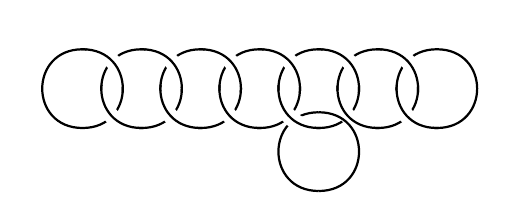
\begin{tikzpicture}
    \begin{knot}[clip width=7]
      \strand[thick] (0,0)
        to [out=left,in=left,looseness=1.75] (0,1)
        to [out=right,in=right,looseness=1.75] (0,0);
      \strand[thick] (0.75,0)
        to [out=left,in=left,looseness=1.75] (0.75,1)
        to [out=right,in=right,looseness=1.75] (0.75,0);
      \strand[thick] (1.5,0)
        to [out=left,in=left,looseness=1.75] (1.5,1)
        to [out=right,in=right,looseness=1.75] (1.5,0);
      \strand[thick] (2.25,0)
        to [out=left,in=left,looseness=1.75] (2.25,1)
        to [out=right,in=right,looseness=1.75] (2.25,0);
      \strand[thick] (3,0)
        to [out=left,in=left,looseness=1.75] (3,1)
        to [out=right,in=right,looseness=1.75] (3,0);
      \strand[thick] (3.75,0)
        to [out=left,in=left,looseness=1.75] (3.75,1)
        to [out=right,in=right,looseness=1.75] (3.75,0);
      \strand[thick] (4.5,0)
        to [out=left,in=left,looseness=1.75] (4.5,1)
        to [out=right,in=right,looseness=1.75] (4.5,0);
      \flipcrossings{1,3,5,7,9,11}
      \strand[thick] (3,-0.8)
        to [out=left,in=left,looseness=1.75] (3,0.2);
    \end{knot}
    \begin{knot}
      \strand[thick] (3,0.2)
        to [out=right,in=right,looseness=1.75] (3,-0.8);
    \end{knot}
  \end{tikzpicture}
\] Imagine this model as living in \(S^3\). Next, hollow out all these
rings: actually delete the portion of space that lies inside them! We
now have a 3-manifold \(M\) whose boundary \(\partial M\) consists of 8
connected components, each a torus. Of course, a solid torus also has a
torus as its boundary. So attach solid tori to each of these 8
components of \(\partial M\), but do it via this attaching map:
\[(x,y) \mapsto (y,-x+2y)\] where \(x\) and \(y\) are the obvious
coordinates on the torus, numbers between \(0\) and \(2\pi\), and we do
the arithmetic \(\mod 2\pi\). We now have a new 3-manifold without
boundary\ldots{} and this is the Poincare homology sphere.

We see here a strange and indirect connection between \(\mathrm{E}_8\)
and the dodecahedron. This is not the only such connection! There's also
the ``McKay correspondence'' (see \protect\hyperlink{week65}{``Week
65''}) and a way of getting the \(\mathrm{E}_8\) root lattice from the
``icosians'' (see \protect\hyperlink{week20}{``Week 20''}).

Are these three superficially different connections secretly just
different views of the same grand picture? I'm not sure. I think I'd
know the answer to part of this puzzle if I better understood the
relation between ADE theory and singularities.

But Diarmuid Crowley told me much more. The Poincare homology sphere is
actually the boundary of a 4-manifold, and it's not hard to say what
this 4-manifold is. I just gave you a recipe for cutting out 8 solid
tori from the 3-sphere and gluing them back in with a twist. Suppose we
think of 3-sphere as the boundary of the 4-disk \(D^4\), and think of
each solid torus as part of the boundary of a copy of
\(D^2 \times D^2\), using the fact that
\[\partial(D^2\times D^2) = S^1\times D^2 + D^2\times S^1.\] Then the
same recipe can be seen as instructions for gluing 8 copies of
\(D^2\times D^2\) to the 4-ball along part of their boundary, getting a
new 4-manifold with boundary. If you ponder it, you'll see that the
boundary of this 4-manifold is the Poincare homology 3-sphere.

Now, this is actually no big deal, at least for folks who know some
3-dimensional topology. But Crowley likes higher-dimensional topology,
and what he told me is this: the whole story generalizes to higher
dimensions! Instead of starting with this picture of linked 1-spheres in
the 3-sphere: \[
  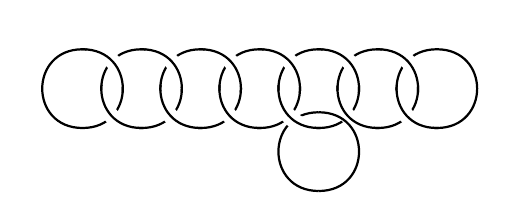
\begin{tikzpicture}
    \begin{knot}[clip width=7]
      \strand[thick] (0,0)
        to [out=left,in=left,looseness=1.75] (0,1)
        to [out=right,in=right,looseness=1.75] (0,0);
      \strand[thick] (0.75,0)
        to [out=left,in=left,looseness=1.75] (0.75,1)
        to [out=right,in=right,looseness=1.75] (0.75,0);
      \strand[thick] (1.5,0)
        to [out=left,in=left,looseness=1.75] (1.5,1)
        to [out=right,in=right,looseness=1.75] (1.5,0);
      \strand[thick] (2.25,0)
        to [out=left,in=left,looseness=1.75] (2.25,1)
        to [out=right,in=right,looseness=1.75] (2.25,0);
      \strand[thick] (3,0)
        to [out=left,in=left,looseness=1.75] (3,1)
        to [out=right,in=right,looseness=1.75] (3,0);
      \strand[thick] (3.75,0)
        to [out=left,in=left,looseness=1.75] (3.75,1)
        to [out=right,in=right,looseness=1.75] (3.75,0);
      \strand[thick] (4.5,0)
        to [out=left,in=left,looseness=1.75] (4.5,1)
        to [out=right,in=right,looseness=1.75] (4.5,0);
      \flipcrossings{1,3,5,7,9,11}
      \strand[thick] (3,-0.8)
        to [out=left,in=left,looseness=1.75] (3,0.2);
    \end{knot}
    \begin{knot}
      \strand[thick] (3,0.2)
        to [out=right,in=right,looseness=1.75] (3,-0.8);
    \end{knot}
  \end{tikzpicture}
\] start with an analogous pattern of 8 \(n\)-spheres linked in the
\((2n+1)\)-sphere. Do all the same stuff, boosting the dimensions
appropriately\ldots{} and you'll get an interesting (2n+1)-dimensional
manifold \(\partial M\) which is the boundary of a (2n+2)-dimensional
manifold M.

When n is \emph{odd} and greater than 1, this manifold \(\partial M\) is
actually an ``exotic sphere''. In other words, it's homeomorphic but not
diffeomorphic to the usual sphere of dimension 2n+1.

Now, exotic spheres of a given dimension form an abelian group G under
connected sum (see \protect\hyperlink{week141}{``Week 141''}). This
group consists of two parts: the easy part and the hard part. The easy
part is a normal subgroup \(N\) consisting of the exotic spheres that
bound parallelizable smooth manifolds. The size of this subgroup can be
computed in terms of Bernoulli numbers and stuff like that. The hard
part is the quotient group \(G/N\). This is usually the cokernel of a
famous gadget called the ``\(J\)-homomorphism''. I say ``usually''
because this is known to be true in most dimensions, but in certain
dimensions it remains an open question.

Anyway: the easy part \(N\) is always a finite cyclic group, and this is
\emph{generated} by the exotic sphere \(\partial M\) that I just
described!

For example:

In dimension 7 we have \(G = N = \mathbb{Z}/28\), so there are 28 exotic
spheres in this dimension (up to orientation-preserving diffeomorphism),
and they are all connected sums of the exotic 7-sphere \(\partial M\)
formed by the above construction.

In dimension 11 we have \(G = N = \mathbb{Z}/992\), so there are 992
exotic spheres, and they are all connected sums of the exotic 11-sphere
\(\partial M\) formed by the above construction.

In dimension 15 we no longer have \(G = N\). Instead we have
\(N = \mathbb{Z}/8128\) and \(G = \mathbb{Z}/8128\oplus \mathbb{Z}/2\).
There are thus 16256 exotic spheres in this dimension, only half of
which are connected sums of the exotic 15-sphere \(\partial M\) formed
by the above construction.

And so on.

While we're on the subject of exotic 15-spheres, I can't resist
mentioning this. I explained in \protect\hyperlink{week141}{``Week
141''} how to construct a bunch of exotic 7-spheres (24 of them,
actually) using the quaternions. Once you understand this trick, it's
natural to wonder if you can construct exotic 15-spheres the same way,
but using octonions instead of quaternions. Well, you can:

\begin{enumerate}
\def\labelenumi{\arabic{enumi})}
\setcounter{enumi}{2}
\tightlist
\item
  Nobuo Shimada, ``Differentiable structures on the 15-sphere and
  Pontrjagin classes of certain manifolds'', \emph{Nagoya Math. Jour.}
  \textbf{12} 1957, 59--69.
\end{enumerate}

I should also explain what I really like about the above stuff. In
topological quantum field theory, people like to get 3-manifolds by
``surgery on framed links''. The idea is to start with a framed link in
the 3-sphere, use the framing to thicken each component to an embedded
solid torus, cut out these solid tori, and reattach them ``the other
way'', using the fact that \(S^1\times S^1\) is the boundary of both
\(S^1\times D^2\) and \(D^2\times S^1\). We can get any compact oriented
3-manifold this way.

The above construction of the Poincare homology sphere was just an
example of this, where the link was \[
  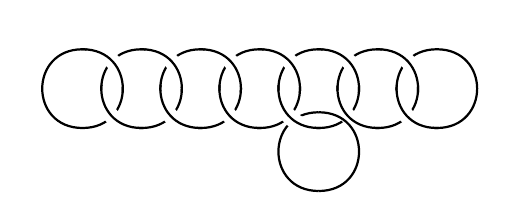
\begin{tikzpicture}
    \begin{knot}[clip width=7]
      \strand[thick] (0,0)
        to [out=left,in=left,looseness=1.75] (0,1)
        to [out=right,in=right,looseness=1.75] (0,0);
      \strand[thick] (0.75,0)
        to [out=left,in=left,looseness=1.75] (0.75,1)
        to [out=right,in=right,looseness=1.75] (0.75,0);
      \strand[thick] (1.5,0)
        to [out=left,in=left,looseness=1.75] (1.5,1)
        to [out=right,in=right,looseness=1.75] (1.5,0);
      \strand[thick] (2.25,0)
        to [out=left,in=left,looseness=1.75] (2.25,1)
        to [out=right,in=right,looseness=1.75] (2.25,0);
      \strand[thick] (3,0)
        to [out=left,in=left,looseness=1.75] (3,1)
        to [out=right,in=right,looseness=1.75] (3,0);
      \strand[thick] (3.75,0)
        to [out=left,in=left,looseness=1.75] (3.75,1)
        to [out=right,in=right,looseness=1.75] (3.75,0);
      \strand[thick] (4.5,0)
        to [out=left,in=left,looseness=1.75] (4.5,1)
        to [out=right,in=right,looseness=1.75] (4.5,0);
      \flipcrossings{1,3,5,7,9,11}
      \strand[thick] (3,-0.8)
        to [out=left,in=left,looseness=1.75] (3,0.2);
    \end{knot}
    \begin{knot}
      \strand[thick] (3,0.2)
        to [out=right,in=right,looseness=1.75] (3,-0.8);
    \end{knot}
  \end{tikzpicture}
\] and each component had two twists in the framing as we go around, as
compared to the standard ``blackboard'' framing. This is why there was
that mysterious number ``2'' in my formula for the attaching map.

Whenever we describe a 3-manifold using ``surgery on framed links'' this
way, there's an important matrix where the entry in the \(i\)th row and
\(j\)th column is the linking number of the \(i\)th component and the
\(j\)th component of our framed link, with the diagonal entries standing
for the ``self-linking'' numbers of the components, that is, the number
of twists their framings have. This matrix is important because it also
describes the ``intersection form'' on the 2nd homology group of a
simply-connected 4-manifold \(M\) whose boundary \(\partial M\) is the
3-manifold we're describing.

For example, in the case of the Poincare homology sphere, this matrix is
called the \(\mathrm{E}_8\) Cartan matrix: \[
  \left(
    \begin{array}{rrrrrrrr}
      2&-1&0&0&0&0&0&0
    \\-1&2&-1&0&0&0&0&0 
    \\0&-1&2&-1&0&0&0&0 
    \\0&0&-1&2&-1&0&0&0 
    \\0&0&0&-1&2&-1&0&-1
    \\0&0&0&0&-1&2&-1&0
    \\0&0&0&0&0&-1&2&0 
    \\0&0&0&0&-1&0&0&2
    \end{array}
  \right)
\] The Dynkin diagram simply summarizes this matrix in pictorial form. I
already described the 4-manifold \(M\) whose boundary is the Poincare
homology sphere; now you know its intersection form.

Anyway, what I find exciting is that all this stuff generalizes to
higher dimensions if we restrict attention to manifolds that have
trivial homotopy groups up to a certain point! For example, it works for
compact oriented smooth 7-manifolds that have trivial \(\pi_1\) and
\(\pi_2\). Any such manifold can be obtained by doing surgery on some
framed 3-spheres embedded in \(S^7\). Just as 1-spheres can link in 3d
space since 1+1 is one less than 3, 3-spheres can link in 7d space since
3+3 is one less than 7. We again get a matrix of linking numbers. As
before, this matrix is also an intersection form: namely, the
intersection form on the 4th homology group of an 8-manifold M whose
boundary \(\partial M\) is the 7-manifold we're describing. Moreover,
this matrix is symmetric in both the 3-manifold example and the
7-manifold example, since it describes an intersection pairing on an
\emph{even-dimensional} homology group.

Even better, all the same stuff happens in manifolds with enough trivial
homotopy groups in dimension 11, and dimension 15\ldots{} and all
dimensions of the form \(4n-1\). And what's \emph{really} neat is that
these higher-dimensional generalizations are in some ways simpler than
the 3d story. The reason is that a 1-sphere can be knotted in 3-space in
really complicated ways, but the higher-dimensional generalizations do
not involve such complicated knotting. The framing aspects can be more
complicated, since there's more to framing an embedded sphere than just
an integer, but it's not all \emph{that} complicated.

So maybe I can learn some more 3d topology by first warming up with the
simpler 7d case\ldots.

Finally, I'd like to list a few articles that I've been meaning to read,
but haven't gotten around to. I hope to read them sometime \emph{this}
millennium! I'll quote the abstracts and make a few comments.

\begin{enumerate}
\def\labelenumi{\arabic{enumi})}
\setcounter{enumi}{3}
\tightlist
\item
  Jack Morava, ``Cobordism of symplectic manifolds and asymptotic
  expansions'', a talk at the conference in honor of S.P. Novikov's 60th
  birthday, available as
  \href{https://arxiv.org/abs/math.SG/9908070}{\texttt{math.SG/9908070}}.
\end{enumerate}

\begin{quote}
The cobordism ring of symplectic manifolds defined by V.L. Ginzburg is
shown to be isomorphic to the Pontrjagin ring of complex-oriented
manifolds with free circle actions. This suggests an interpretation of
the formal group law of complex cobordism, in terms of a composition-law
on semiclassical expansions. An appendix discusses related questions
about cobordism of toric varieties.
\end{quote}

I started trying to explain the relation between formal group laws and
complex oriented cohomology theories in
\protect\hyperlink{week150}{``Week 150''}, because I'm quite puzzled
about the deep inner meaning of this relation. This paper might be the
key to this mystery!

\begin{enumerate}
\def\labelenumi{\arabic{enumi})}
\setcounter{enumi}{4}
\tightlist
\item
  Detlev Buchholz, ``Current trends in axiomatic quantum field theory'',
  available as
  \href{https://arxiv.org/abs/hep-th/9811233}{\texttt{hep-th/9811233}}.
\end{enumerate}

\begin{quote}
In this article a non-technical survey is given of the present status of
Axiomatic Quantum Field Theory and interesting future directions of this
approach are outlined. The topics covered are the universal structure of
the local algebras of observables, their relation to the underlying
fields and the significance of their relative positions. Moreover, the
physical interpretation of the theory is discussed with emphasis on
problems appearing in gauge theories, such as the revision of the
particle concept, the determination of symmetries and statistics from
the superselection structure, the analysis of the short distance
properties and the specific features of relativistic thermal states.
Some problems appearing in quantum field theory on curved spacetimes are
also briefly mentioned.
\end{quote}

I've been falling behind on new developments in axiomatic quantum field
theory. Lots of cool stuff is happening, I hear. This might help me
catch up.

\begin{enumerate}
\def\labelenumi{\arabic{enumi})}
\setcounter{enumi}{5}
\tightlist
\item
  Matt Visser, ``The reliability horizon'', available as
  \href{https://arxiv.org/abs/gr-qc/9710020}{\texttt{gr-qc/9710020}}.
\end{enumerate}

\begin{quote}
The ``reliability horizon'' for semi-classical quantum gravity
quantifies the extent to which we should trust semi-classical quantum
gravity, and gives a handle on just where the ``Planck regime'' resides.
The key obstruction to pushing semi-classical quantum gravity into the
Planck regime is often the existence of large metric fluctuations,
rather than a large back-reaction.
\end{quote}

This seems like a very sensible enterprise: determining just where
semiclassical calculations are likely to break down, and quantum gravity
effects to become important. Why haven't I read this? It's obviously
worthwhile!

\begin{enumerate}
\def\labelenumi{\arabic{enumi})}
\setcounter{enumi}{6}
\tightlist
\item
  Bianca Letizia Cerchiai and Julius Wess, ``\(q\)-Deformed Minkowski
  Space based on a \(q\)-Lorentz Algebra'', available as
  \href{https://arxiv.org/abs/math.QA/9801104}{math.QA/9801104}.
\end{enumerate}

\begin{quote}
The Hilbert space representations of a non-commutative \(q\)-deformed
Minkowski space, its momenta and its Lorentz boosts are constructed. The
spectrum of the diagonalizable space elements shows a lattice-like
structure with accumulation points on the light-cone.
\end{quote}

The \(q\)-deformed Lorentz algebra plays a role in quantum gravity with
nonzero cosmological constant, but it also shows up in noncommutative
geometry. Are the two roles related? I don't know! This is on my list of
puzzles to ponder.

The people applying the \(q\)-deformed Lorentz algebra to noncommutative
geometry want to develop the theory of \(q\)-deformed Minkowski space,
see if it makes the infinities in quantum field theory go away, and see
what physical predictions it makes. It makes spacetime discrete in a
very pretty way; that I know from Julius Wess' talk in Schladming a few
years back (see \protect\hyperlink{week129}{``Week 129''}). But I should
learn more about this, and not just because Bianca Letizia Cerchiai is a
very nice person who invited my girlfriend and I to lunch at her
parents' apartment in Milan\ldots. oh, now I'm feeling \emph{terribly}
guilty for not reading her paper! How nasty of me! I'd better print it
out and read it as soon as I go into the office!

In fact, now that I think of it, I've had at least \emph{some} dealings
with \emph{all} the authors of these papers. And now I'm publicly
admitting I haven't read some of their most interesting papers! Ugh! At
least this admission may shame me into reading them now\ldots{}

Bye.

\begin{center}\rule{0.5\linewidth}{0.5pt}\end{center}

On \texttt{sci.physics.research}, Aaron Bergman clarified something
about these millennial physics problems:

\begin{quote}
John Baez wrote:
\end{quote}

\begin{quote}
\begin{quote}
Aaron Bergman (abergman@Princeton.EDU) wrote:
\end{quote}
\end{quote}

\begin{quote}
\begin{quote}
\begin{quote}
John Baez wrote:
\end{quote}
\end{quote}
\end{quote}

\begin{quote}
\begin{quote}
\begin{quote}
\begin{quote}
Of course, this business of limiting ``physics'' to mean ``the search
for fundamental laws'' annoys condensed matter physicists like Philipp
Anderson, since it excludes everything they work on.
\end{quote}
\end{quote}
\end{quote}
\end{quote}

\begin{quote}
\begin{quote}
\begin{quote}
One should note that Gross explicitly says --- there's a Realaudio of
the talk online --- that this is a very narrowminded list that excludes
fundamental questions in other fields. It's not really intended to be a
universal list.
\end{quote}
\end{quote}
\end{quote}

\begin{quote}
\begin{quote}
Good! It's too bad the text of the webpage doesn't make that clearer.
I'm appending your comment to the version of ``week164'' on my website,
assuming you don't object.
\end{quote}
\end{quote}

\begin{quote}
Sure. Or you can just refer them to the transparencies and the talk. For
those who don't want to bother listening to the whole thing, start
listening at about 7:30 mins into the RealAudio stream:

http://feynman.physics.lsa.umich.edu/cgi-bin/s2ktalk.cgi?questions

It's on transparency 4 which is why I mentioned,
\end{quote}

\begin{quote}
\begin{quote}
\begin{quote}
And Witten is coming back.
\end{quote}
\end{quote}
\end{quote}

\begin{quote}
\begin{quote}
You mean he's not staying in LA? Can't take the winters out here?
\end{quote}
\end{quote}

\begin{quote}
I won't speculate on the reasons, but his grad students have said that
he's coming back to the Institute.

\hypertarget{aaron}{%
\subsection{Aaron}\label{aaron}}

Aaron Bergman
\end{quote}

\begin{center}\rule{0.5\linewidth}{0.5pt}\end{center}
\hypertarget{week165}{%
\section{DATE}\label{week165}}

A few weeks ago I went to the University of Wisconsin at Milwaukee to
give some talks at their Center for Gravitation and Cosmology. They have
a group of 8 people working on data analysis for the LIGO experiment. As
you probably know, LIGO will use laser interferometry to look for
gravitational waves. It consists of two detectors, one near Livingston,
Louisiana, and one near Hanford, Washington. Each one is shaped like an
L, with each arm of the L consisting of a 4-kilometer-long evacuated
pipe with a laser beam running down it. A typical gravitational wave
might stretch one of the arms by \(10^{-16}\) centimeters --- one
hundred-millionth of the diameter of a hydrogen atom. It will be quite
exciting if they can actually get this level of precision. They're not
there yet, but already they can tell when wind-blown tumbleweeds pile up
along the pipe at the Hanford site, because their gravitational pull
bends the beam and messes things up!

In Milwaukee, it's a time of preparation and anticipation. The first
data should start coming in by September, but right now they're busy
writing software and assembling a ``Beowulf cluster''. This is a
parallel computer formed from a bunch of commercially available
processors, all running Linux. I'd heard about these before, because my
friend Dan Christensen is planning to do calculations in spin foam
models of quantum gravity on a Beowulf cluster over at the University of
Western Ontario. The cluster at Milwaukee will have 128 processors, each
with at least 1 gigaflop peak performance, and a total of 19 terabytes
of distributed disk memory.

You can learn more about this at their homepage:

\begin{enumerate}
\def\labelenumi{\arabic{enumi})}
\tightlist
\item
  University of Wisconsin at Milwaukee, Center for Gravitation and
  Cosmology home page, \texttt{http://www.gravity.phys.uwm.edu/}
\end{enumerate}

For a nice popular account of the LIGO experiment, try this:

\begin{enumerate}
\def\labelenumi{\arabic{enumi})}
\setcounter{enumi}{1}
\tightlist
\item
  Marcia Bartusiak, \emph{Einstein's Unfinished Symphony: Listening to
  the Sounds of Space-Time}, Joseph Henry Press, Washington D.C., 2000.
\end{enumerate}

My host was at Milwaukee was John Friedman. I was surprised and pleased
to find that he was one of the people who discovered how to make
spin-\(1/2\) particles out of topological defects in spacetime!
Theoretically speaking, that is. I'd heard about this trick, but I never
knew where it came from:

\begin{enumerate}
\def\labelenumi{\arabic{enumi})}
\setcounter{enumi}{2}
\tightlist
\item
  J. Friedman and R. Sorkin, ``Spin \(1/2\) from gravity'', \emph{Phys.
  Rev.~Lett.} \textbf{44} (1980), 1100.
\end{enumerate}

I was more familiar with a recent implementation of it in the framework
of loop quantum gravity, as mentioned in
\protect\hyperlink{week128}{``Week 128''}.

Friedman and Sorkin's trick was based on the idea of ``dyons''. I'd
never understood dyons, but Friedman explained them to me, and now the
idea seems so simple that I can't resist telling everyone.

To make a ``dyon'', just take a charged particle and a magnetic monopole
and tape them together with high-quality duct tape. You can buy all
these materials at your local hardware store\ldots{} though mine was out
of monopoles when I last checked.

Now, rotate your dyon. As you move the charged particle around the
monopole, it picks up a phase, thanks to the magnetic field.
Alternatively, as you move the monopole around charged particle, it
picks up a phase thanks to the electric field! Either way, you get the
same phase when you move one of these guys all the way around the other
--- and this phase has to be \(1\) or \(-1\) for well-known topological
reasons. If the phase is \(1\), your dyon is a boson. But if the phase
is \(-1\), your dyon is a fermion!

In short, this is a strange and interesting way to build fermions out of
components that are not themselves fermionic.

In Milwaukee, I gave a talk where I tried to explain the meaning of
Einstein's equation in simple English. There are a lot of books that
give simple explanations of curved spacetime, geodesics and so on.
Unfortunately, most of them don't explain the real meat of general
relativity: Einstein's equation. This bugs me, especially since it's not
so hard. If you're interested, take a look at this:

\begin{enumerate}
\def\labelenumi{\arabic{enumi})}
\setcounter{enumi}{3}
\tightlist
\item
  John Baez, ``The meaning of Einstein's equation'', available at
  \href{https://arxiv.org/abs/gr-qc/0103044}{\texttt{gr-qc/0103044}}.
\end{enumerate}

Since my Milwaukee trip I've become really busy writing notes on the
quantum gravity seminar here at Riverside. Toby Bartels and I have been
writing them up in the form of a rather silly dialog, and my student
Miguel Carrion-Alvarez has been been writing them in a more traditional
format. Eventually they will be put together in the form of a book, but
it's a lot of work. That's the main reason This Week's Finds has been
dormant lately. You can see all these notes here:

\begin{enumerate}
\def\labelenumi{\arabic{enumi})}
\setcounter{enumi}{4}
\tightlist
\item
  John Baez, Toby Bartels and Miguel Carrion, \emph{Quantum Gravity
  Seminar}, \texttt{http://math.ucr.edu/home/baez/qg.html}
\end{enumerate}

The ultimate goal is to describe spin foam models of 4d quantum gravity,
but we're only gradually working our way to that point.

There are a lot of other things I'd like to talk about, but I don't have
time to do them all justice. For example, there's a nice new book of
essays on quantum gravity:

\begin{enumerate}
\def\labelenumi{\arabic{enumi})}
\setcounter{enumi}{5}
\tightlist
\item
  Craig Callender and Nick Huggett, eds., \emph{Physics Meets Philosophy
  at the Planck Scale: Contemporary Theories in Quantum Gravity},
  Cambridge U. Press, Cambridge, 2001.
\end{enumerate}

It has articles by Chris Isham, Carlo Rovelli, Ed Witten and other
folks. I found Gordon Belot and John Earman's ``Pre-Socratic Quantum
Gravity'' to be a particularly clear-headed account of the so-called
``problem of time'' in quantum gravity. I wish it had existed when I was
first struggling to understand this subject! Everyone trying to
understand quantum gravity should read this.

Over on the more technical end, Martin Bojowald has written a bunch of
papers applying loop quantum gravity to the big bang, which I want to
catch up with:

\begin{enumerate}
\def\labelenumi{\arabic{enumi})}
\setcounter{enumi}{6}
\item
  Martin Bojowald, ``Loop Quantum Cosmology I: Kinematics'',
  \emph{Class. Quant. Grav.} \textbf{17} (2000), 1489--1508, also
  available at
  \href{https://arxiv.org/abs/gr-qc/9919103}{\texttt{gr-qc/9919103}}

  ``Loop Quantum Cosmology II: Volume Operators'', \emph{Class. Quant.
  Grav.} \textbf{17} (2000), 1509--1526, also available at
  \href{https://arxiv.org/abs/gr-qc/9910104}{\texttt{gr-qc/9910104}}.

  ``Loop Quantum Cosmology III: Wheeler-DeWitt Operators'', \emph{Class.
  Quant. Grav.} \textbf{18} (2001), 1055--1070, also available at
  \href{https://arxiv.org/abs/gr-qc/0008052}{\texttt{gr-qc/0008052}}.

  ``Loop Quantum Cosmology IV: Discrete Time Evolution'', \emph{Class.
  Quant. Grav.} \textbf{18} (2001) 1071--1088, also available at
  \href{https://arxiv.org/abs/gr-qc/0008053}{\texttt{gr-qc/0008053}}.

  ``Absence of Singularity in Loop Quantum Cosmology'', available at
  \href{https://arxiv.org/abs/gr-qc/0102069}{\texttt{gr-qc/0102069}}.
\end{enumerate}

The really interesting ones are the last two, whose titles explain why
they're interesting --- but they're based on the framework developed in
the earlier papers.

And then there's \(n\)-category theory! Two of Martin Hyland's students
have been making interesting progress on this subject. Tom Leinster has
been studying operads, their generalizations, their relation to homotopy
theory, and their application to \(n\)-categories. He's even given a new
definition of ``weak \(n\)-category'', thus adding to the profusion of
competing candidates:

\begin{enumerate}
\def\labelenumi{\arabic{enumi})}
\setcounter{enumi}{7}
\item
  Tom Leinster, ``General operads and multicategories'', available as
  \href{https://arxiv.org/abs/math.CT/9810053}{\texttt{math.CT/9810053}}.

  \emph{Structures in higher-dimensional category theory}, Ph.D.~thesis,
  available at
  \texttt{http://www.dpmms.cam.ac.uk/\textasciitilde{}leinster/shdctabs.html}

  ``Up-to-homotopy monoids'', available as
  \href{https://arxiv.org/abs/math.QA/9912084}{\texttt{math.QA/9912084}}.

  ``Homotopy algebras for operads'', available as
  \href{https://arxiv.org/abs/math.QA/0002180}{\texttt{math.QA/0002180}}.

  ``Operads in higher-dimensional category theory'', available as
  \href{https://arxiv.org/abs/math.CT/0011106}{\texttt{math.CT/0011106}}
\end{enumerate}

Eugenia Cheng, on the other hand, seems to be working to \emph{reduce}
the number of different definitions of weak \(n\)-category, by laying
the groundwork for connecting various existing definitions --- mainly
those based on ``opetopes'' and related shapes:

\begin{enumerate}
\def\labelenumi{\arabic{enumi})}
\setcounter{enumi}{8}
\item
  Eugenia Cheng, ``The relationship between the opetopic and multitopic
  approaches to weak \(n\)-categories'', available at
  \texttt{http://www.dpmms.cam.ac.uk/\textasciitilde{}elgc2/}

  ``Equivalence between approaches to the theory of opetopes'',
  available at
  \texttt{http://www.dpmms.cam.ac.uk/\textasciitilde{}elgc2/}
\end{enumerate}

I'm glad these energetic young folks are stepping in to help out the
older folks like me who have become completely exhausted from thinking
about \(n\)-categories.

Finally, everyone who wants to understand M-theory and its relation to
matrix models should first read this review article by Nicolai and
Helling:

\begin{enumerate}
\def\labelenumi{\arabic{enumi})}
\setcounter{enumi}{9}
\tightlist
\item
  Hermann Nicolai and Robert Helling, ``Supermembranes and M(atrix)
  theory'', available as
  \href{https://arxiv.org/abs/hep-th/9809103}{\texttt{hep-th/9809103}}.
\end{enumerate}

and then this new review article by Wati Taylor:

\begin{enumerate}
\def\labelenumi{\arabic{enumi})}
\setcounter{enumi}{9}
\tightlist
\item
  Washington Taylor, ``M(atrix) theory: matrix quantum mechanics as a
  fundamental theory'', available as
  \href{https://arxiv.org/abs/hep-th/0101126}{\texttt{hep-th/0101126}}.
\end{enumerate}

They're both pretty cool. How does a theory of matrices wind up acting
like a theory of membranes? That's what you'll understand if you study
this stuff.

\begin{center}\rule{0.5\linewidth}{0.5pt}\end{center}
\hypertarget{week166}{%
\section{DATE}\label{week166}}

Do you know this number?
\[2.685452001065306445309714835481795693820382293994462953051152\ldots\]
They say that mathematics is not really about numbers, and they're
right. But sometimes it's fun to play around with the darn things!

Given any positive number you can work out its continued fraction
expansion, like this:
\[\sqrt{2} = 1+\frac{1}{2+\frac{1}{2+\frac{1}{2+_{\ldots}}}}\] But
normally it won't look so pretty! A number is rational if and only if
the continued fraction stops after finitely many steps. If its continued
fraction expansion eventually repeats, like this:
\[\sqrt{3} = 1+\frac{1}{1+\frac{1}{2+\frac{1}{1+_{\ldots}}}}\] then it
satisfies a quadratic equation with integer coefficients. So the
continued fraction expansion of e can't ever repeat\ldots{} but it's
cute nonetheless:
\[e = 2+\frac{1}{1+\frac{1}{2+\frac{1}{1+\frac{1}{1+\frac{1}{4+\frac{1}{1+\frac{1}{1+\frac{1}{6+_{\ldots}}}}}}}}}\]
It continues on predictably after that initial hiccup. The number
\(\pi\), on the other hand, gives a random-looking mess. This is a hint
that \(\pi\) is number-theoretically more complicated than \(e\), which
is also apparent when you compare the proofs that \(e\) and \(\pi\) are
transcendental --- the proof for \(e\) is much easier.

Pondering all this, it's natural to ask about the ``average'' behavior
of the continued fraction expansion of a number. What's the average
behavior of the series \(a_1, a_2, a_3, \ldots\) that we get this way:
\[x=a_1+\frac{1}{a_2+\frac{1}{a_3+\frac{1}{a_4+_{\ldots}}}}\] It turns
out that if we take the geometric mean of the first \(n\) terms and then
let \(n\) approach \(\infty\), the mean almost always converges to
``Khinchin's constant'' --- the number at the beginning of this article!
Here by ``almost always'' I mean that the set of exceptions has measure
zero. One can prove this using some ideas from ergodic theory.

Now, there is much more to say about continued fraction expansions, but
my real goal is simply to point out that there are lots of interesting
constants in mathematics besides \(\pi\), \(e\), the golden ratio, and
Euler's number. Where can you read about them? Here:

\begin{enumerate}
\def\labelenumi{\arabic{enumi})}
\tightlist
\item
  Steven Finch, ``MathSoft Constants'',
  \texttt{http://pauillac.inria.fr/algo/bsolve/constant/constant.html}
\end{enumerate}

This is a great place to learn about Khinchin's constant, Feigenbaum's
number, Madelung's constant, Artin's constant, Grothendieck's constant,
and many other fun numbers!

Speaking of fun websites, here's another:

\begin{enumerate}
\def\labelenumi{\arabic{enumi})}
\setcounter{enumi}{1}
\tightlist
\item
  The Mathematics Genealogy Project,
  \texttt{http://hcoonce.math.mankato.msus.edu/}
\end{enumerate}

My advisor's advisor's advisor's advisor's advisor's advisor's advisor's
advisor was Gauss. If you think I'm showing off, you're right! But I
couldn't have done it without this website, and if you're a
mathematician, there's a good chance you use it to track down
\emph{your} academic lineage. And if you can't, you can at least add
your information to the database.

Before Demian Cho showed me this site, I'd gotten stuck 3 generations
back in my attempts to discover my academic ancestors. Now I can go back
11 generations. I know it's annoying, but I'm gonna tell you the whole
story:

My advisor was Irving Segal, the guy who helped prove the
Gelfand-Naimark-Segal theorem. This is a basic result about
\(C^*\)-algebras, a kind of gadget he invented to formalize the notion
of an ``algebra of observables'' in quantum theory. The GNS theorem
implies that every \(C^*\)-algebra sits inside the algebra of all
bounded operators on some Hilbert space, so it's a kind of justification
for using Hilbert spaces in quantum physics. But even better, it gives a
procedure for representing a \(C^*\)-algebra as operators on a Hilbert
space starting from a ``state'' on the \(C^*\)-algebra. The upshot is
that while Hilbert spaces are important, the right Hilbert space to use
can depend on the state of the system you're studying. At first people
thought Segal was nuts for saying this, but by now it's well-accepted.

Segal also did work on quantum field theory, nonlinear partial
differential equations, and other topics at the borderline between
physics and functional analysis. His students include Isadore Singer and
Bertram Kostant, whose work on geometric quantization generalized
Segal's ideas on the ``Bargmann-Segal representation''. I worked with
Segal because I liked analysis and wanted to understand quantum field
theory in a rigorous way.

Segal's advisor was Einar Hille, the guy who helped prove the
Hille-Yosida theorem. Hille did a lot of work on integral and
differential equations, but later he became interested in functional
analysis: the study of infinite-dimensional vector spaces equipped with
nice topologies, such as Hilbert spaces, Banach spaces and the like. At
the time, he was rather special in his emphasis on applying these
abstract ideas to concrete problems. In his book ``Methods in Classical
and Functional Analysis,'' he wrote:

\begin{quote}
If the book has a thesis, it is that a functional analyst is an analyst,
first and foremost, and not a degenerate species of a topologist. His
problems come from analysis and his results should throw light on
analysis\ldots.
\end{quote}

The Hille-Yosida theorem shows how to write a large class of
one-parameter semigroups of linear operators on Banach spaces in the
form \(\exp(-tH)\). These so-called ``contraction semigroups'' naturally
come from the heat equation and its relatives. Segal was fond of this
idea, and he generalized it to semigroups of nonlinear operators, which
arise naturally from \emph{nonlinear} partial differential equations. He
used this idea to prove global existence of solutions for various
nonlinear classical field theories.

Hille's advisor was Marcel Riesz, the guy who didn't prove the Riesz
representation theorem. Marcel's brother Frigyes was the guy who did
that. Marcel worked on functional analysis, partial differential
equations, and mathematical physics --- even Clifford algebras and
spinors!

The advisor of Marcel Riesz was Lipot Fejer, the guy who discovered the
Fejer kernel. This shows up when you sum Fourier series. If you just
naively sum the Fourier series of a continuous function on the circle,
it may not converge uniformly. However, if you use a trick called Cesaro
summation, which amounts to averaging the partial sums, you get uniform
convergence. The average of the first \(n\) partial sums of the Fourier
series of your function is equal to its convolution with the Fejer
kernel. Fejer also worked on conformal mappings. His students included
Paul Erdos and Gabor Szego.

Fejer's advisor was Karl Herman Amandus Schwarz, the guy who helped
prove the Cauchy-Schwarz inequality. That's a wonderful inequality which
everyone should know! But Schwarz also worked on minimal surfaces and
complex analysis: for example, conformal mappings from polyhedra into
the sphere, and also the Dirichlet problem. Don't mix him up with
Laurent Schwartz, the guy who invented distributions.

(Actually, Lipot Fejer's name was originally Leopold Weiss. He changed
it to seem more Hungarian. This was a common practice at the time in
Hungary, but when he did it, his advisor Schwarz stopped speaking to
him!)

Schwarz's advisor was Karl Weierstrass, the guy who proved the
Weierstrass theorem. This theorem says that every continuous real-valued
function on the unit interval is a uniform limit of polynomials.
Weierstrass also has a function named after him: the Weierstrass
elliptic function, which I explained in
\protect\hyperlink{week13}{``Week 13''}. But his real claim to fame is
how he made analysis more rigorous! For example, he discovered the
importance of uniform convergence, and found a continuous function with
no derivative at any point. Besides Schwarz, his students include
Frobenius, Killing, and Kowalevsky.

Now, Weierstrass doesn't have an advisor listed in the mathematics
genealogy. However, by using this website full of mathematician's
biographies, I can go back further:

\begin{enumerate}
\def\labelenumi{\arabic{enumi})}
\setcounter{enumi}{2}
\tightlist
\item
  John J. O'Connor and Edmund F. Robertson, ``The MacTutor History of
  Mathematics Archive'',
  \texttt{http://www-groups.dcs.st-andrews.ac.uk/\textasciitilde{}history/index.html}
\end{enumerate}

According to this, Weierstrass had an erratic career as a student: his
father tried to make him study finance instead of math, so he spent his
undergraduate years fencing and drinking. He learned a lot of math on
his own, and got really interested in elliptic functions from the work
of Abel and Jacobi. I can't tell if he ever had an official dissertation
advisor. However, in 1839 he went to the Academy at Muenster to study
under Christoph Gudermann, who worked on elliptic functions and
spherical geometry. Gudermann strongly encouraged Weierstrass in his
mathematical studies. Weierstrass asked for a question on elliptic
functions, and wound up writing a paper which Gudermann assessed
``\ldots{} of equal rank with the discoverers who were crowned with
glory.'' (When Weierstrass heard this, he commended Gudermann's
generosity, since he had strongly criticized Gudermann's methods.)

Given all this, and the fact that Weierstrass seems to have had no
\emph{other} mentor, I'll declare Gudermann to be his advisor, de facto
even if not officially.

But who was Gudermann? He's the guy they named the ``gudermannian''
after! That's this function:
\[\mathrm{gd}(u) = 2 \arctan(\exp(u)) - \frac\pi2.\] Now, if you're
wondering why such a silly function deserves a name, you should work out
its inverse function: \[\mathrm{gd}^{-1}(x) = \ln(\sec(x) + \tan(x)).\]
And if you don't recognize \emph{this}, you probably haven't taught
freshman calculus lately! It's the integral of \(\sec(x)\), which is one
of the hardest of the basic integrals you teach in that kind of course.
But it's not just hard, it's historically important: a point at latitude
\(\mathrm{gd}(u)\) has distance \(u\) from the equator in a Mercator
projection map. If you think about it a while, this is precisely what's
needed to make the projection be a conformal transformation --- that is,
angle-preserving. And that's just what you want if you're sailing a ship
in a constant direction according to a compass and you want to know
where you'll wind up.

If you don't see how this works, try:

\begin{enumerate}
\def\labelenumi{\arabic{enumi})}
\setcounter{enumi}{3}
\tightlist
\item
  Wikipedia, \texttt{http://en.wikipedia.org/wiki/Mercator\_projection}
\end{enumerate}

Gudermann's advisor was Carl Friedrich Gauss, the guy they named
practically \emph{everything} after! Poor Gudermann, who was content to
mess around with special functions and spherical geometry, seems to have
been one of Gauss' worst students. But that's not so bad, since three of
the other four were Bessel, Dedekind and Riemann.

Gauss' advisor was Johann Pfaff, the guy they named the ``Pfaffian''
after. If the matrix A is skew-symmetric, we can write
\[\det(A) = \operatorname{Pf}(A)^2\] where \(\operatorname{Pf}(A)\) is
also a polynomial in the entries of \(A\). Pfaffians now show up in the
study of fermionic wavefunctions. Pfaff worked on various things,
including the integrability of partial differential equations, where the
concept of a ``Pfaffian system'' is important. Unfortunately I've never
gotten around to understanding these.

Pfaff's advisor was Abraham Kaestner. I'd never heard of him before now.
He wrote a 4-volume history of mathematics, but his most important work
was on axiomatic geometry. His interest in the parallel postulate
indirectly got Gauss, Bolyai and Lobachevsky interested in that topic:
we've already seen that he taught Gauss' advisor, but he also taught
Bolyai's father, as well as Lobachevsky's teacher, one J. M. C. Bartels.
In fact, Kaestner was still teaching when Gauss went to school, but
Gauss didn't go to Kaestner's courses, because he found them too
elementary. Gauss said of him, ``He is the best poet among
mathematicians and the best mathematician among poets''. Perhaps this
faint praise refers to Kaestner's knack for aphorisms.

At this point I got stuck until my student Miguel Carrion-Alvarez helped
out. It appears that Kaestner's advisor was one Christian A. Hausen.
He's the guy they named the Hausen crater after --- a lunar crater
located at 65.5 S, 88.4 W. He did his thesis on theology in 1713, but
became a professor of mathematics in Leipzig. He worked on
electrostatics, but made no memorable discoveries.

At this point the trail disappears into mist. For some conjectures, see
this page:

\begin{enumerate}
\def\labelenumi{\arabic{enumi})}
\setcounter{enumi}{4}
\tightlist
\item
  Anthony M. Jacobi, ``Academic Family Tree'',
  \texttt{http://www.staff.uiuc.edu/\%7Ea-jacobi/tree.html}
\end{enumerate}

It's interesting how the same themes keep popping up in this genealogy.
For example, Weierstrass invented uniform convergence and proved that
the limit of a uniformly convergent series of continuous functions is
continuous. The Fejer kernel shows up when you're trying to write
functions on the circle as a uniformly convergent sum of complex
exponentials. Segal's \(C^*\)-algebras generalize the notion of uniform
convergence to operator algebras. I guess these things just go from
generation to generation\ldots.

A little while ago John McKay visited me and told me about all sorts of
wonderful things: relations between subgroups of the Monster group,
exceptional Lie groups, and modular forms\ldots{} a presentation of the
Monster group with 2 generators, a way to build the Leech lattice from 3
copies of the \(\mathrm{E}_8\) lattice\ldots{} a way to get ahold of the
Monster group starting with a diagram with 26 nodes\ldots.

Unfortunately, I'm having trouble finding references for some of these
things! It's possible that the last two items are really these:

\begin{enumerate}
\def\labelenumi{\arabic{enumi})}
\setcounter{enumi}{5}
\item
  Robert L. Griess, ``Pieces of eight: semiselfdual lattices and a new
  foundation for the theory of Conway and Mathieu groups''. \emph{Adv.
  Math.} \textbf{148} (1999), 75--104.
\item
  John H. Conway, Christopher S. Simons, ``26 implies the Bimonster'',
  \emph{Jour. Algebra} \textbf{235} (2001), 805--814.
\end{enumerate}

Anyway, I need to read about this stuff.

Speaking of exceptionology: in \protect\hyperlink{week163}{``Week 163''}
I explained how \(\mathrm{Spin}(9)\) sits inside the Lie group
\(\mathrm{F}_4\), thanks to the fact that \(\mathrm{Spin}(9)\) is the
automorphism group of Jordan algebra of \(2\times2\) hermitian
octonionic matrices, and \(\mathrm{F}_4\) is the automorphism group of
the Jordan algebra of \(3\times\) hermitian matrices. But in fact, since
there are different ways to think of \(2\times2\) matrices as special
\(3\times\) matrices, there are actually 3 equally good ways to stuff
\(\mathrm{Spin}(9)\) in \(\mathrm{F}_4\). Since I'd been hoping this
might be important in particle physics, it was nice to discover that
Pierre Ramond, a real expert on this stuff, has had similar thoughts. In
fact he's written two papers on this! Let me just quote the abstracts:

\begin{enumerate}
\def\labelenumi{\arabic{enumi})}
\setcounter{enumi}{7}
\tightlist
\item
  Pierre Ramond, ``Boson-fermion confusion: the string path to
  supersymmetry'', available at
  \href{https://arxiv.org/abs/hep-th/0102012}{\texttt{hep-th/0102012}}.
\end{enumerate}

\begin{quote}
Reminiscences on the string origins of supersymmetry are followed by a
discussion of the importance of confusing bosons with fermions in
building superstring theories in 9+1 dimensions. In eleven dimensions,
the kinship between bosons and fermions is more subtle, and may involve
the exceptional group \(\mathrm{F}_4\).
\end{quote}

\begin{enumerate}
\def\labelenumi{\arabic{enumi})}
\setcounter{enumi}{8}
\tightlist
\item
  T. Pengpan and Pierre Ramond, M(ysterious) patterns in
  \(\mathrm{SO}(9)\), Phys. Rep.~315 (1999) 137-152, also available as
  \href{https://arxiv.org/abs/hep-th/9808190}{\texttt{hep-th/9808190}}.
\end{enumerate}

\begin{quote}
The light-cone little group, \(\mathrm{SO}(9)\), classifies the massless
degrees of freedom of eleven-dimensional supergravity, with a triplet of
representations. We observe that this triplet generalizes to four-fold
infinite families with the quantum numbers of massless higher spin
states. Their mathematical structure stems from the three equivalent
ways of embedding \(\mathrm{SO}(9)\) into the exceptional group
\(\mathrm{F}_4\).
\end{quote}

\begin{center}\rule{0.5\linewidth}{0.5pt}\end{center}

\begin{quote}
\emph{``This is why we are here,'' said Teacher, ``to be good and kind
to other people.''}

Pippi stood on her head on the horse's back and waved her legs in the
air. ``Heigh-ho,'' said she, ``then why are the other people here?''

--- Astrid Lingren, \emph{Pippi Goes on Board}
\end{quote}
\hypertarget{week167}{%
\section{DATE}\label{week167}}

I'm now visiting the Center for Gravitational Physics and Geometry at
Penn State, and I have all sorts of exciting stuff to report. First I'll
talk about fundamental limitations in measuring distances due to quantum
gravity and then I'll say a bit about Martin Bojowald's new work, which
uses loop quantum gravity to tackle the question ``what came before the
big bang?''

Theoretical physicists sometimes look longingly back to the early 20th
century as the heyday of thought experiments --- Einstein and his
elevator, the famous Bohr-Einstein debate at the 1927 Solvay conference,
and so on. But thought experiments are most important when you're
struggling to do something really new and haven't yet hammered out a
mathematical formalism. The declining importance of thought experiments
in later years is mainly a reflection of the tremendous success of
quantum mechanics and general relativity,

But what about when QM and GR meet?

Here we need all the help we can get. For example: does it make any
sense to do experiments looking for quantum fluctuations in the geometry
of spacetime, or are they far too puny to detect with present
technology? A precise answer would require a full-fledged theory of
quantum gravity, which we don't have. But a rough answer is all we need!
Here's where thought experiments come in handy. However, one must be
careful\ldots{} verbal reasoning easily conceals many pitfalls! Let me
present an argument that puts a lower bound on how accurately we can
measure distances:

\begin{enumerate}
\def\labelenumi{\arabic{enumi})}
\tightlist
\item
  Y. Jack Ng and H. van Dam, ``Measuring the foaminess of space-time
  with gravity-wave interferometers'', \emph{Found. Phys.} \textbf{30}
  (2000) 795--805, also available as
  \href{https://arxiv.org/abs/gr-qc/9906003}{\texttt{gr-qc/9906003}}
\end{enumerate}

You can decide if it's right or not.

First: how accurate can a clock be? One limitation is that any clock has
some position uncertainty. This translates into time uncertainty when we
read the clock by having it send photons to us.

Let's work this out, ignoring factors of \(2\) and small stuff like
that. Suppose our clock has mass \(m\) and starts out with a position
uncertainty equal to \(D\). Then the uncertainty of our clock's momentum
is at least \(\hbar/D\), so its velocity is uncertain by at least
\(\hbar/mD\). After a time \(T\), its position uncertainty will grow to
about \[dx > D + \frac{\hbar t}{mD}.\]

This is minimized when \[D = \left(\frac{\hbar t}{m}\right)^{\frac12}\]
which gives \[dx > \left(\frac{\hbar t}{m}\right)^{\frac12}.\]

This position uncertainty translates into an uncertainty of
\[dt = \frac{dx}{c}\] in the time we read off the clock, so we have
\[c dt > \left(\frac{\hbar t}{m}\right)^{\frac12}.\] Thus, to keep time
with an accuracy \(dt\) over a span of time equal to \(t\), our clock
must have mass \[m > \frac{\hbar t}{c^2 dt^2}.\]

This part of the argument actually goes back to Wigner:

\begin{enumerate}
\def\labelenumi{\arabic{enumi})}
\setcounter{enumi}{1}
\item
  Eugene P. Wigner, ``Relativistic invariance and quantum phenomena'',
  \emph{Rev.~Mod. Phys.} \textbf{29} (1957), 255--268.

  H. Salecker and E. P. Wigner, ``Quantum limitations of the measurement
  of space-time distances'', \emph{Phys. Rev.} \textbf{109}, (1958),
  571--577. Also available at
  \texttt{http://fangio.magnet.fsu.edu/\textbackslash{}\textasciitilde{}vlad/pr100/100\ yrs/html/chap14\_toc.htm}
\end{enumerate}

Next: how accurate can a distance measurement be? Suppose we measure the
distance between two clocks by timing how long it takes light to go from
one to the other (or make a round trip, if you prefer). If our clocks
keep time with accuracy \(dt\), the uncertainty in the distance
measurement is \[dx = c dt\] Of course, our clocks must keep time this
accurately long enough for light to get from one to the other, so their
masses must satisfy \[m > \frac{\hbar t}{c^2 dt^2}\] or
\[m > \frac{\hbar t}{dx^2}.\]

If \(x\) is the distance between the clocks, we have \[x = c t\] so this
gives \[m > \frac{\hbar x}{c dx^2}.\tag{$\star$}\] In short, to measure
distances accurately this way, our clocks must be heavy.

We've used quantum mechanics. Now let's put gravity into the picture! If
our clocks are \emph{too} heavy they'll collapse into a black hole,
ruining the experiment. This puts a limit on our ability to measure
distances accurately.

To get somewhere with this idea, let's assume the distance \(x\) is
basically the size of our whole experimental apparatus. This must exceed
the Schwarzschild radius for the mass \(m\), or we'll get a black hole,
so we need: \[x > \frac{G m}{c^2}.\] Plugging this into the right-hand
side of (\(\star\)), we get \[m > \frac{\hbar G m}{c^3 dx^2}\] or
\[dx > \left(\frac{\hbar G}{c^3}\right)^{\frac12} = L\] where \(L\) is
the Planck length. So we can't measure distances more accurately than
the Planck length.

Whoops! The last paragraph here is not the argument due to Ng and van
Dam! It's something I came up just now while trying to copy their
argument. Their actual argument is different. They assume the
uncertainty \(dx\) must exceed the Schwarzschild radius of a black hole
of mass \(m\), so that \[dx > \frac{G m}{c^2}.\] If we plug this into
(\(\star\)) and fiddle around, we get \[dx > x^{\frac13} L^{\frac23}.\]
This is much more exciting, because it says that the uncertainty due to
quantum gravity gets bigger when we measure long distances!

Now, the way I've presented Ng and van Dam's argument, the obvious weak
spot is their assumption that the uncertainty in position measurement is
greater than the radius of a black hole with mass equal to that of the
experimental apparatus. Where does this assumption come from? They get
it by saying the clocks ``tick'' once each time light bounces back and
forth between them. If the clocks' accuracy is limited by their tick
rate, we have \(dt = t\) and thus \(dx = x\), so my assumption
\[x > \frac{G m}{c^2}\] turns into their stronger assumption
\[dx > \frac{G m}{c^2}\]

But to me it seems artificial, even circular, to measure distances using
clocks that work this way!

For further criticism of this argument, see:

\begin{enumerate}
\def\labelenumi{\arabic{enumi})}
\setcounter{enumi}{2}
\tightlist
\item
  Ronald J. Adler, Ilya M. Nemenman, James M. Overduin, David I.
  Santiago, ``On the detectability of quantum spacetime foam with
  gravitational-wave interferometers'', \emph{Phys. Lett.} \textbf{B477}
  (2000) 424--428, also available at
  \href{https://arxiv.org/abs/gr-qc/9909017}{\texttt{gr-qc/9909017}}.
\end{enumerate}

For their response, see:

\begin{enumerate}
\def\labelenumi{\arabic{enumi})}
\setcounter{enumi}{3}
\tightlist
\item
  Y. Jack Ng and H. van Dam, ``On Wigner's clock and the detectability
  of spacetime foam with gravitational-wave interferometers'',
  \emph{Phys. Lett.} \textbf{B477} (2000) 429--435, also available at
  \href{https://arxiv.org/abs/gr-qc/9911054}{\texttt{gr-qc/9911054}}.
\end{enumerate}

For an argument that claims an even larger value of the position
uncertainty, namely \[dx > x^{\frac12} L^{\frac12},\] see these papers:

\begin{enumerate}
\def\labelenumi{\arabic{enumi})}
\setcounter{enumi}{4}
\item
  G. Amelino-Camelia, ``Quantum theory's last challenge'', \emph{Nature}
  \textbf{408} (2000) 661--664.

  ``Testable scenario for relativity with minimum length'', available at
  \href{https://arxiv.org/abs/hep-th/0012238}{\texttt{hep-th/0012238}}
\end{enumerate}

Let's do a little number-crunching to compare these calculations. An
gravitational wave detector like LIGO is basically just a device that
bounces a laser between mirrors to carefully measure the distance
between them. The goal of LIGO is to measure a 4-kilometer distance with
a precision of \(10^{-18}\) meters. If we believe the fundamental
uncertainty in distance measurements is about the Planck length, LIGO
has no chance of bumping into this limit, since the Planck length is
about \(10^{-35}\) meters. If we believe Ng and van Dam's thought
experiment, we get an uncertainty of about \(10^{-22}\) meters. If we
believe Amelino-Camelia's argument, we get a figure of about
\(10^{-16}\) meters\ldots{} which would be very noticeable at LIGO!

Unfortunately, I'm pretty sure the Planck length figure is about right.
For another derivation of this figure, see:

\begin{enumerate}
\def\labelenumi{\arabic{enumi})}
\setcounter{enumi}{5}
\tightlist
\item
  Ronald J. Adler and David I. Santiago, ``On gravity and the
  uncertainty principle'', \emph{Mod. Phys. Lett.} \textbf{A14} (1999)
  1371, also available at
  \href{https://arxiv.org/abs/gr-qc/9904026}{\texttt{gr-qc/9904026}}.
\end{enumerate}

What other ways might we detect quantum gravity effects? One is to look
for dispersion of light as it passes through the vacuum. Maxwell's
equations say that in the vacuum the speed of light is independent of
its wavelength. But if spacetime is ``grainy'' at short distance scales,
this might not be exactly correct. If the velocity were
frequency-dependent, a pulse of radiation would get slightly smeared out
as it travels along through empty space.

There are calculations in both string theory and loop quantum gravity
which raise this as a possibility:

\begin{enumerate}
\def\labelenumi{\arabic{enumi})}
\setcounter{enumi}{6}
\item
  J. Ellis, N.E. Mavromatos and D. V. Nanopoulos, ``Search for quantum
  gravity'', \emph{Gen.~Rel. Grav.} \textbf{31} (1999) 1257--1262, also
  available as
  \href{https://arxiv.org/abs/gr-qc/9905048}{\texttt{gr-qc/9905048}}.
\item
  Jorge Pullin and Rodolfo Gambini, ``Nonstandard optics from quantum
  spacetime'', \emph{Phys. Rev.} \textbf{D59} (1999) 124021, also
  available as
  \href{https://arxiv.org/abs/gr-qc/9809038}{\texttt{gr-qc/9809038}}.
\end{enumerate}

These calculations are quite controversial. For one thing, they require
a breaking of Lorentz invariance, since there's no way to get the speed
of light to depend on its wavelength without picking out a special rest
frame. This makes some people's hair stand on end.

But never mind: suppose we were looking for this effect. Nobody has seen
it yet, so it must be tiny if it exists at all. To detect it we'd want
our light to travel a long distance\ldots{} say, 10 billion light years.
And we'd like a source that emitted a pulse of light whose variation in
time we can detect with good resolution\ldots{} say, less than a
millisecond.

Hmm. How can we arrange this? Use \(\gamma\)-ray bursters! We don't have
to build them; nature has seen to that, so we can use these rascals to
put limits on this dispersion effect. For more details, try:

\begin{enumerate}
\def\labelenumi{\arabic{enumi})}
\setcounter{enumi}{8}
\tightlist
\item
  J. Ellis, K. Farakos, N.E. Mavromatos, V. Mitsou and D.V. Nanopoulos,
  ``Astrophysical probes of the constancy of the velocity of light'',
  \emph{Astrophys. J.} \textbf{535} (2000) 139--151, also available as
  \href{https://arxiv.org/abs/astro-ph/9907340}{\texttt{astro-ph/9907340}}.
\end{enumerate}

So far, nobody has seen quantum gravity effects this way.

Okay\ldots{} let me wrap things up with a word about Martin Bojowald's
work on quantum cosmology. I listed his papers in
\protect\hyperlink{week165}{``Week 165''}, but didn't get around to
discussing them.

From an outsider's viewpoint, the exciting thing about this work is that
it uses loop quantum gravity to study what happened before the big bang.
And the answer is simple: there was a big crunch! In other words,
Bojowald can extrapolate the quantum version of the big bang cosmology
back before \(t = 0\), without encountering any singularity, and he gets
a collapsing universe which shrinks down to zero volume at \(t = 0\)
before re-expanding in a big bang.

From an insider's perspective, the exciting thing is that he's using
loop quantum gravity to study dynamics. Since loop quantum gravity is
background-free, there's no Hamiltonian, just a Hamiltonian constraint.
This means that any study of dynamics must confront the thorny ``problem
of time'': how to do physics without a god-given external clock that's
outside the system you're studying. And this problem makes it hard to
tell which formula for the Hamiltonian constraint is ``right''. Thiemann
came up with a candidate for the Hamiltonian constraint back in 1996
(see \protect\hyperlink{week85}{``Week 85''}), and the field has
struggled ever since to make up it's collective mind about this formula,
without much success so far.

Bojowald's progress comes from looking at ``minisuperspace models'',
where we assume the universe is highly symmetrical --- as people often
do in cosmology. This allows him to tackle the problem of time by
treating the volume of the universe as a notion of time. It's like
having one aspect of the system you're studying be the clock that you
use to see how other things change. This idea per se is not new; what's
new is carrying it out in the framework of loop quantum gravity. In loop
quantum gravity volume is discrete\ldots{} so Bojowald's ``clock'' ticks
in discrete steps. By adapting Thiemann's formula for the Hamiltonian
constaint to this highly symmetrical context, he can write it as an
evolution equation saying how other observables change as a function of
the volume of the universe. Since volume is discrete, this equation is a
difference equation rather than a differential equation.

He can solve this equation on the computer\ldots{} and he finds that
even when the universe is very small, on the order of the Planck length,
it closely mimics the classically expected behavior. However, there is
no singularity at \(t = 0\), or more precisely, at zero volume.

Here's where things get technical, in a way that tickles me pink, but
may bore you to tears:

A funny feature of the volume operator in loop quantum gravity is that
it's expressed in terms of the square root of the absolute value of a
certain quantity. We can think of this quantity as a sort of ``volume
squared'' operator, but with both positive and negative eigenvalues.
This always used to puzzle me, and I've put a lot of thought into this
issue. Renate Loll has also written a paper about it. I'm delighted to
find that in Bojowald's setup, it becomes a real \emph{virtue} of loop
quantum gravity, since it allows us to extrapolate our quantum cosmology
to negative times --- or more precisely, negative ``volume squared''!

How can you visualize this? Crudely speaking, negative-volume-squared
states of the universe can be thought of as ``inside-out versions'' of
positive-volume-squared ones. So the way I visualize Bojowald's result
is like this: the universe shrinks to nothing as you rewind history back
to the big bang, and then expands again ``inside out'' as you go to
negative times.

Anyway, regardless of how we visualize it, loop quantum gravity is now
at the stage of making dynamical predictions about serious physics
questions. Ashtekar and Bojowald are now working to determine what
happens at the singularity of a black hole\ldots{} so stay tuned!

\begin{center}\rule{0.5\linewidth}{0.5pt}\end{center}

\emph{Now the thing about time is that time isn't really real. It's just
your point of view, how does it feel for you? Einstein said he could
never understand it all.} --- James Taylor
\hypertarget{week168}{%
\section{DATE}\label{week168}}

It's been about two months since the last issue of This Week's Finds,
and I apologize for this. I've been very busy, and my limited writing
energy has all gone into finishing up a review article on the octonions.
I'm dying to talk about that\ldots{} but first things first!

When I left off I was at Penn State, learning about the latest
developments in quantum gravity. I told you how Martin Bojowald was
using loop quantum gravity to study what came before the big
bang\ldots{} but I didn't mention that he'd written a nice little book
on the subject:

\begin{enumerate}
\def\labelenumi{\arabic{enumi})}
\tightlist
\item
  Martin Bojowald, \emph{Quantum Geometry and Symmetry}, Shaker Verlag,
  Aachen, 2000. Available at
  \texttt{http://www.shaker.de/Online-Gesamtkatalog/Details.asp?ISBN=3-8265-7741-8}
\end{enumerate}

This does not cover his most recent work, in which his program is really
starting to pay off\ldots{} but it will certainly help you
\emph{understand} his recent work. He's doing lots of great stuff these
days. In fact, he just came out with a paper yesterday:

\begin{enumerate}
\def\labelenumi{\arabic{enumi})}
\setcounter{enumi}{1}
\tightlist
\item
  Martin Bojowald, ``The semiclassical limit of loop quantum
  cosmology'', available at
  \href{https://arxiv.org/abs/gr-qc/0105113}{\texttt{gr-qc/0105113}}.
\end{enumerate}

This explains how his new approach to quantum cosmology is related to
the old ``minisuperspace'' approach. In the old approach, you just take
some limited class of cosmologies satisfying the equations of general
relativity and think of this class as a classical mechanics problem with
finitely many degrees of freedom: for example, the size of the universe
together with various numbers describing its shape. Then you quantize
this classical system.

In this approach, you don't see any hint of spacetime discreteness on
the Planck scale. But in Bojowald's approach, you do! What gives? He
still starts with a limited class of cosmologies and quantizes that, but
he does so using ideas taken from loop quantum gravity. This makes all
the difference: now areas and volumes have discrete spectra of
eigenvalues, and this saves us from the horrors of the singularity at
the big bang. In fact, we can go back \emph{before} the big bang, and
find a time-reversed expanding universe on the other side!

But what's the relation between this new approach and the old one,
exactly? Well, in loop quantum gravity, space is described using ``spin
networks'', and area is quantized. Each edge of a spin network is
labelled by some spin \(j = 0, 1/2, 1, \ldots\), and when a spin-\(j\)
edge punctures a surface, it gives that surface an area equal to
\[8\pi\gamma\sqrt{j(j+1)}\] times the Planck length squared. Here
\(\gamma\) is a constant called the ``Immirzi parameter'' --- see
\protect\hyperlink{week112}{``Week 112''} and
\protect\hyperlink{week148}{``Week 148''} for more about that. Bojowald
shows that you can recover the old approach to quantum cosmology from
his new one by taking a limit in which the Immirzi parameter approaches
zero while the spins labelling spin network edges go to infinity. In
this limit, the spacings between the above areas go to zero --- so the
discrete spectrum of the ``area operator'' becomes continuous! Thus we
lose the discrete geometry which is typical of loop quantum gravity.

I'm also excited by what's going on with spin foams lately. For one, my
friend Dan Christensen is starting to do numerical calculations with the
Riemannian Barrett-Crane model. I've discussed this model in
\protect\hyperlink{week113}{``Week 113''},
\protect\hyperlink{week120}{``Week 120''}, and
\protect\hyperlink{week128}{``Week 128''}, so I won't bore you with the
details yet again. For now, let me just say that it's a theory of
quantum gravity in which spacetime is a triangulated 4-dimensional
manifold. There is also a Lorentzian version of this model, which is
more physical, but it's trickier to compute with, so Dan has wisely
decided to start by tackling the Riemannian version.

As you probably know, in quantum field theory, as in statistical
mechanics, the partition function is king. So Dan Christensen is
starting out by using a supercomputer to numerically calculate the
partition function of a triangulated 4-sphere. He has some students
helping him, and he's also gotten some help from Greg Egan\ldots.

Anyway: this partition function is a sum over all ways of labelling
triangles by spins --- but it's not obvious that the sum converges! For
this reason Dan has begun by imposing a ``cutoff'', that is, an upper
bound on the allowed spins. Physically this would be called an
``infrared cutoff'', since big spins mean big triangles. The question
is: what happens as you let this cutoff approach infinity? Does the
partition function converge or not?

Now, what's cool is that in November of last year, a fellow named
Alejandro Perez claimed to have proven that it \emph{does} converge:

\begin{enumerate}
\def\labelenumi{\arabic{enumi})}
\setcounter{enumi}{2}
\tightlist
\item
  Alejandro Perez, ``Finiteness of a spin foam model for euclidean
  quantum general relativity'', \emph{Nucl. Phys.} \textbf{B599} (2001)
  427--434. Also available at
  \href{https://arxiv.org/abs/gr-qc/0011058}{\texttt{gr-qc/0011058}}.
\end{enumerate}

I say ``claimed'', not because I doubt his proof, but because I still
haven't checked it, and I should. But the great thing is: now we have
both numerical and analytic ways of studying this spin foam model, and
we can play them off against each other! This helps a lot when you're
trying to understand a complicated problem.

Of course, the skeptics among you will say ``Fine, but this is just
Riemannian quantum gravity, not the Lorentzian theory. We're still not
talking about the real world.'' And you'd be right! But luckily, there
has also been a lot of progress on the Lorentzian Barrett-Crane model.

This version of the Barrett-Crane model is based on the Lorentz group
instead of the rotation group. Because the representations of the
Lorentz group are parametrized in a continuous rather than discrete way,
in this version one computes the partition function as as an
\emph{integral} over ways of labelling the triangles by nonnegative real
numbers. These numbers represent areas, so it seems that area is not
quantized in this theory --- but I should warn you, this is a hotly
debated issue! We need to better understand how this model relates to
loop quantum gravity, where area is quantized.

Anyway, when Barrett and Crane proposed the Lorentzian version of their
model, it wasn't obvious that this integral for the partition function
converged. Even worse, it wasn't clear that the integrand was
well-defined! The basic ingredient in the integrand is the so-called
``Lorentzian \(10j\) symbol'', which describes the amplitude for an
individual 4-simplex to have a certain geometry, as specified by the
areas of its 10 triangular faces. Barrett and Crane wrote down an
explicit integral for the Lorentzian \(10j\) symbol, but they didn't
show this integral converges.

Last summer, in a fun-filled week of intense calculation, John Barrett
and I showed that the integral defining the Lorentzian \(10j\) symbols
\emph{does} in fact converge:

\begin{enumerate}
\def\labelenumi{\arabic{enumi})}
\setcounter{enumi}{3}
\tightlist
\item
  John Baez and John W. Barrett, ``Integrability for relativistic spin
  networks'', available at
  \href{https://arxiv.org/abs/gr-qc/0101107}{\texttt{gr-qc/0101107}}.
\end{enumerate}

It took us until this January to write up those calculations. By April,
Louis Crane, Carlo Rovelli, and Alejandro Perez had written a paper
extending our methods to show that the partition function converges:

\begin{enumerate}
\def\labelenumi{\arabic{enumi})}
\setcounter{enumi}{4}
\tightlist
\item
  Louis Crane, Alejandro Perez, Carlo Rovelli, ``A finiteness proof for
  the Lorentzian state sum spin foam model for quantum general
  relativity'', available as
  \href{https://arxiv.org/abs/gr-qc/0104057}{\texttt{gr-qc/0104057}}.
\end{enumerate}

So now we have a well-defined quantum gravity theory for a 4-dimensional
spacetime with a fixed triangulation, and we can start studying it! The
big question is whether it mimics general relativity at distance scales
much larger than the Planck scale.

But enough of that. Now: octonions!

I've finally finished writing a survey of the octonions and their
connections to Clifford algebras and spinors, Bott periodicity,
projective and Lorentzian geometry, Jordan algebras, the exceptional Lie
groups, quantum logic, special relativity and supersymmetry:

\begin{enumerate}
\def\labelenumi{\arabic{enumi})}
\setcounter{enumi}{5}
\tightlist
\item
  John Baez, ``The octonions'',
  \texttt{http://math.ucr.edu/home/baez/octonions/}. Also available at
  \href{http://www.arXiv.org/abs/math.RA/0105155}{\texttt{math.RA/0105155}}.
\end{enumerate}

Let me just sketch some of the main themes. For details and precise
statements, read the paper!

Octonions arise naturally from the interaction between vectors and
spinors in 8-dimensional Euclidean space, but in superstring theory and
other physics applications, what matters most is their relation to
10-dimensional Lorentzian spacetime. This is part of a pattern:

\begin{enumerate}
\def\labelenumi{\arabic{enumi})}
\tightlist
\item
  spinors in 1d Euclidean space are real numbers (\(\mathbb{R}\)).
\item
  spinors in 2d Euclidean space are complex numbers (\(\mathbb{C}\)).
\item
  spinors in 4d Euclidean space are quaternions (\(\mathbb{H}\)).
\item
  spinors in 8d Euclidean space are octonions (\(\mathbb{O}\)).
\end{enumerate}

(These numbers are just the dimensions of \(\mathbb{R}\),
\(\mathbb{C}\), \(\mathbb{H}\) and \(\mathbb{O}\).)

Also:

\begin{enumerate}
\def\labelenumi{\arabic{enumi})}
\tightlist
\item
  points in 3d Minkowski spacetime are \(2\times2\) hermitian real
  matrices
\item
  points in 4d Minkowski spacetime are \(2\times2\) hermitian complex
  matrices
\item
  points in 6d Minkowski spacetime are \(2\times2\) hermitian
  quaternionic matrices
\item
  points in 10d Minkowski spacetime are \(2\times2\) hermitian
  octonionic matrices
\end{enumerate}

(These numbers are 2 more than the dimensions of \(\mathbb{R}\),
\(\mathbb{C}\), \(\mathbb{H}\) and \(\mathbb{O}\).)

The octonions are also what lie behind the 5 exceptional simple Lie
groups. The exceptional group \(\mathrm{G}_2\) is just the symmetry
group of the octonions. The other four exceptional groups, called
\(\mathrm{F}_4\), \(\mathrm{E}_6\), \(\mathrm{E}_7\) and
\(\mathrm{E}_8\), are symmetry groups of ``projective planes'' over:

\begin{enumerate}
\def\labelenumi{\arabic{enumi})}
\tightlist
\item
  the octonions, \(\mathbb{O}\)
\item
  the complexified octonions or ``bioctonions'',
  \(\mathbb{C}\otimes\mathbb{O}\)
\item
  the quaternionified octonions or ``quateroctonions'',
  \(\mathbb{H}\otimes\mathbb{O}\)
\item
  the octonionified octonions or ``octooctonions'',
  \(\mathbb{O}\otimes\mathbb{O}\)
\end{enumerate}

respectively.

Warning: I put the phrase ``projective planes'' in quotes here because
the last two spaces are not projective planes in the usual axiomatic
sense (see \protect\hyperlink{week145}{``Week 145''}). This makes the
subject a bit tricky.

Now, it is no coincidence that:

\begin{enumerate}
\def\labelenumi{\arabic{enumi})}
\tightlist
\item
  spinors in 9-dimensional Euclidean space are pairs of octonions.
\item
  spinors in 10-dimensional Euclidean space are pairs of bioctonions.
\item
  spinors in 12-dimensional Euclidean space are pairs of
  quateroctonions.
\item
  spinors in 16-dimensional Euclidean space are pairs of octooctonions.
\end{enumerate}

(These numbers are 8 more than the dimensions of \(\mathbb{R}\),
\(\mathbb{C}\), \(\mathbb{H}\) and \(\mathbb{O}\).)

This sets up a relation between spinors in these various dimensions and
the projective planes over \(\mathbb{O}\),
\(\mathbb{C}\otimes\mathbb{O}\), \(\mathbb{H}\otimes\mathbb{O}\) and
\(\mathbb{O}\otimes\mathbb{O}\). The upshot is that we get a nice
description of \(\mathrm{F}_4\), \(\mathrm{E}_6\), \(\mathrm{E}_7\) and
\(\mathrm{E}_8\) in terms of the Lie algebras \(\mathfrak{so}(n)\) and
their spinor representations where \(n = 9, 10, 12, 16\), respectively.

It's all so tightly interlocked --- I can't believe it's not trying to
tell us something about physics! Just to whet your appetite for more,
Just to whet your appetite for more, let me show you 7 quateroctonionic
descriptions of the Lie algebra of \(\mathrm{E}_7\): \[
  \begin{aligned}
    \mathfrak{e}_7
    &= \mathfrak{isom}((\mathbb{H}\otimes\mathbb{O})\mathbb{P}^2)
  \\&= \mathfrak{der}(\mathrm{h}_3(\mathbb{O}))\oplus\mathrm{h}_3(\mathbb{O})^3
  \\&= \mathfrak{der}(\mathbb{O})\oplus\mathfrak{der}(\mathrm{h}_3(\mathbb{H}))\oplus(\Im(\mathbb{O})\otimes\mathrm{sh}_3(\mathbb{H}))
  \\&= \mathfrak{der}(\mathbb{H})\oplus\mathfrak{der}(\mathrm{h}_3(\mathbb{O}))\oplus(\Im(\mathbb{H})\otimes\mathrm{sh}_3(\mathbb{O}))
  \\&= \mathfrak{der}(\mathbb{O})\oplus\mathfrak{der}(\mathbb{H})\oplus\mathrm{sa}_3(\mathbb{H}\otimes\mathbb{O})
  \\&= \mathfrak{so}(\mathbb{O}\oplus\mathbb{H})\oplus\Im(\mathbb{H})\oplus(\mathbb{H}\otimes\mathbb{O})^2
  \\&= \mathfrak{so}(\mathbb{O})\oplus\mathfrak{so}(\mathbb{H})\oplus\Im(\mathbb{H})\oplus(\mathbb{H}\otimes\mathbb{O})^3
  \end{aligned}
\] I explain why these are true in the paper, but for now, let me just
say what all this stuff means:

\begin{itemize}
\tightlist
\item
  ``\(\mathfrak{isom}\)'' means the Lie algebra of the isometry group,
\item
  \((\mathbb{H}\otimes\mathbb{O})\mathbb{P}^2\) means the
  quateroctonionic projective plane with its god-given Riemannian
  metric,
\item
  ``\(\mathfrak{der}\)'' means the Lie algebra of derivations,
\item
  \(\mathrm{h}_3(\mathbb{O})\) is the exceptional Jordan algebra,
  consisting of \(3\times3\) hermitian octonionic matrices,
\item
  \(\mathrm{h}_3(\mathbb{H})\) is the Jordan algebra of \(3\times3\)
  hermitian quaternionic matrices,
\item
  \(\Im(\mathbb{O})\) is the 7-dimensional space of imaginary octonions,
\item
  \(\Im(\mathbb{H})\) is the 3-dimensional space of imaginary
  quaternions,
\item
  \(\mathrm{sh}_3(\mathbb{O})\) is the traceless \(3\times3\) hermitian
  octonionic matrices,
\item
  \(\mathrm{sh}_3(\mathbb{H})\) is the traceless \(3\times3\) hermitian
  quaternionic matrices,
\item
  \(\mathrm{sa}_3(\mathbb{H}\otimes\mathbb{O})\) is the traceless
  \(3\times3\) antihermitian quateroctonionic matrices.
\item
  \(\mathfrak{so}(V)\) is the rotation group Lie algebra associated to
  the real inner product space \(V\).
\end{itemize}

It is fun to compute the dimension of \(\mathrm{E}_7\) using each of
these 7 formulas and see that you get 133 each time!

I also give 6 bioctonionic descriptions of \(\mathrm{E}_6\). Alas, I
could not find 8 octooctonionic descriptions of \(\mathrm{E}_8\),
probably because this group is more symmetrical and in a curious sense
simpler than the others.

Time for dinner.

\begin{center}\rule{0.5\linewidth}{0.5pt}\end{center}

\emph{``Don't take life too serious, it ain't nohow permanent.''} ---
Walt Kelly, Pogo
\hypertarget{week169}{%
\section{DATE}\label{week169}}

When I write This Week's Finds as rarely as I do these days, so much
stuff builds up that I completely despair of ever getting to all of
it\ldots{} so I'll just randomly mention a few cool things that are on
the top of my mind right now.

First of all, here's a great new review article on spin foams. If you're
trying to understand spin foam models of quantum gravity, this is the
place to start:

\begin{enumerate}
\def\labelenumi{\arabic{enumi})}
\tightlist
\item
  Daniele Oriti, ``Spacetime geometry from algebra: spin foam models for
  non-perturbative quantum gravity'', \emph{Rep.~Prog. Phys.}
  \textbf{64} (2001), 1489--1544. Also available at
  \href{https://arxiv.org/abs/gr-qc/0106091}{\texttt{gr-qc/0106091}}.
\end{enumerate}

You'll learn how spin foam models naturally show up in all sorts of
different approaches to quantum gravity: loop quantization, path
integral approaches, lattice field theory, matrix models, and
category-theoretic approaches.

Secondly, here's a great introduction to \(n\)-categories and topology:

\begin{enumerate}
\def\labelenumi{\arabic{enumi})}
\setcounter{enumi}{1}
\tightlist
\item
  Tom Leinster, ``Topology and higher-dimensional category theory: the
  rough idea'', available at
  \href{https://arxiv.org/abs/math.CT/0106240}{\texttt{math.CT/0106240}}.
\end{enumerate}

As he says, this is a ``Friday-afternoonish description of some of the
dreams people have for higher-dimensional category theory and its
interactions with topology''. Much more readable than the
Monday-morningish papers where people put in all the details!

And next, here is some stuff I have been thinking about lately.

As you're probably sick to death of hearing, I'm interested in category
theory and also normed division algebras: the real numbers, complex
numbers, quaternions and octonions. There's no instantly obvious
relationship between these topics, but naturally I've tried to find one,
since this would let me unify two of my obsessions into one big
super-obsession. I recently made a bunch of progress, thanks to finding
these papers:

\begin{enumerate}
\def\labelenumi{\arabic{enumi})}
\setcounter{enumi}{2}
\item
  Markus Rost, ``On the dimension of a composition algebra'',
  \emph{Documenta Mathematica} \textbf{1} (1996), 209--214. Available at
  \texttt{http://www.mathematik.uni-bielefeld.de/DMV-J/vol-01/10.html}
\item
  Dominik Boos, ``Ein tensorkategorieller Zugang zum Satz von Hurwitz (A
  tensor-categorical approach to Hurwitz's theorem)'',
  \emph{Diplomarbeit ETH Zurich}, March 1998, available at
  \texttt{http://www.mathematik.uni-bielefeld.de/\textasciitilde{}rost/data/boos.pdf}
\end{enumerate}

I'd like to explain what the problem is and how these papers solve it.

Part of the fun of category theory is that it lets you take mathematical
arguments and generalize them to their full extent by finding the proper
context for them: that is, by figuring out in exactly what sort of
category you can carry out the argument. Out of laziness and ignorance,
people usually work in the category of sets as a kind of ``default
setting''. This category has many wonderful features --- it's like a
machine that chops, slices, dices, grates, liquefies and purees --- but
usually you don't need \emph{all} these features to carry out a
particular task. So, one job of a category theorist is to figure out
what features are actually needed in a given situation, and isolate the
kind of category that has those features.

A ``kind of category'' is sometimes called a ``doctrine''. I believe
this term was invented by Lawvere. It must have some technical
definition, but luckily I don't know it, so I will not be restrained by
it here. I'll just talk in a sloppy way about this question: ``in what
doctrine can we define the concept of a normed division algebra?'' It'll
get technical for a while, so most of you may want to leave, but then
some pretty pictures will show up, so make sure to come back then.

First think a minute about ``algebras''. Here by an ``algebra'' I mean a
finite-dimensional real vector space with a not-necessarily-associative
bilinear product and an element that's both the left and right unit for
this product. We can define algebras like this using the category
\(\mathsf{Vect}\) consisting of real vector spaces and linear operators,
without resorting to full power of the category of sets --- as long as
we use the tensor product in \(\mathsf{Vect}\). We start by saying an
algebra is an object \(A\) in \(\mathsf{Vect}\) together with a product
\[m\colon A \otimes A \to A\] and unit \[i\colon I \to A\] where \(I\)
is the unit object for the tensor product --- that is, the real numbers.
In case you're confused: the map \(i\) here is just the linear operator
sending the real number \(1\) to the unit element of \(A\); we're using
a standard trick for expressing \emph{elements} as \emph{maps}. Given
this stuff, we can write the left and right unit laws by saying this
diagram commutes: \[
  \begin{tikzcd}
    I\otimes A
      \dar[swap,"i\otimes1_A"]
    & A
      \lar \rar
      \dar["1_A" description]
    & A\otimes I
      \dar["1_A\otimes i"]
  \\A\otimes A
      \rar[swap,"m"]
    & A
    & A\otimes A
      \lar["m"]
  \end{tikzcd}
\] where the unlabelled arrows are some obvious isomorphisms coming from
the fact that \(I\) is the unit for the tensor product.

Now, this definition could have been stated in \emph{any} category with
tensor products; or more technically, any ``monoidal category''. So the
right doctrine for talking about algebras of this sort is the doctrine
of monoidal categories.

What's the right doctrine for defining \emph{associative} algebras?
Well, we can write down another commutative diagram to state the
associative law: \[
  \begin{tikzcd}[column sep=small,row sep=huge]
    (A\otimes A)\otimes A
      \ar[rr]
      \dar[swap,"m\otimes1_A"]
    && A\otimes(A\otimes A)
      \dar["1_A\otimes m"]
  \\A\otimes A
      \drar[swap,"m"]
    && A\otimes A
      \dlar["m"]
  \\&A&
  \end{tikzcd}
\] where again the unlabelled arrow is the obvious isomorphism. This
works fine in any monoidal category, so the right doctrine is again that
of monoidal categories. But instead of speaking of an ``associative
algebra'' in a monoidal category, folks usually call a gadget of this
sort a ``monoid object'' --- see \protect\hyperlink{week89}{``Week 89''}
for more on this. The reason is that if we take our monoidal category to
be \(\mathsf{Set}\), a monoid object boils down to a ``monoid'': a set
with an associative product and unit element.

Lots of people like groups more than monoids. What's the right doctrine
for defining groups? This time it's definitely NOT the doctrine of
monoidal categories. The reason is that the equational laws satisfied by
inverses in a group: \[
  \begin{aligned}
    g g^{-1} &= 1
  \\g^{-1} g &= 1
  \end{aligned}
\] have duplicated and deleted arguments --- the ``\(g\)'' shows up
twice on the left side and not at all on the right! This is different
from the associative law \[g (h k) = (g h) k\] where each argument shows
up once on each side of the equation.

In a monoidal category we can't ``duplicate'' or ``delete'' arguments:
if \(X\) is an object in a monoidal category, there's no god-given map
from \(X\) to \(X\otimes X\), or from \(X\) to \(1\). This means we
can't use commutative diagrams in a monoidal category to express
equational laws that duplicate or delete arguments.

However, we \emph{can} duplicate and delete arguments if we're in a
``category with finite products'' --- a nice sort of monoidal category
where we \emph{do} have maps from \(X\) to \(X\otimes X\) and from \(X\)
to \(1\). The best example of this is the category of sets, where the
``tensor product'' is just the usual Cartesian product. This is why we
can easily define groups in the category of sets! More generally, we can
define ``group objects'' in any category with finite products.

So, the right doctrine for talking about groups --- or more precisely,
group objects --- is the doctrine of categories with finite products.

By the way, if you think this stuff is too abstract to be useful, take a
peek at \protect\hyperlink{week54}{``Week 54''} and
\protect\hyperlink{week115}{``Week 115''}, where I described how group
objects show up in algebraic topology. But beware: back then I was
engaging in a bit of overkill, and working in the doctrine of
``categories with finite limits''. This more powerful doctrine also lets
you define gadgets with partially defined operations, like ``category
objects''. But for group objects, finite products are all we really
need.

Gradually getting to the point, let us now ask: what's the right
doctrine for talking about \emph{division} algebras? It's definitely
\textbf{not} the doctrine of monoidal categories. It's not even the
doctrine of categories with finite products! The problem is that a
division algebra is defined to be an algebra such that \(xy = 0\)
implies \(x = 0\) or \(y = 0\). This condition is not even an equational
law: it doesn't say some equation holds, it says ``this equation implies
this one or that one''. To express such fancier conditions as
commutative diagrams, we need a more powerful doctrine.

I'm too lazy to figure out exactly what we need, but certainly the
doctrine of ``topoi'' will do. If you don't know what a topos is, give
yourself 40 lashes and read this:

\begin{enumerate}
\def\labelenumi{\arabic{enumi})}
\setcounter{enumi}{4}
\tightlist
\item
  John Baez, ``Topos theory in a nutshell'',
  \texttt{http://math.ucr.edu/home/baez/topos.html}
\end{enumerate}

However, there are lots of reasons to avoid working in such a powerful
doctrine --- basically, it greatly limits the generality with which one
can discuss a subject.

So it's very interesting to see how much better we can do if we're
interesed in \emph{normed} division algebras. These are algebras
equipped with a norm such that \[|xy| = |x| |y|\] and if we're working
in the category of real vector spaces, the only examples are the real
numbers, the complex numbers, the quaternions and the octonions. These
have all sorts of important applications in physics, so it's good to see
what doctrine we need to talk about them.

The problem is that the norm is nothing like a linear map. To get around
this, it's better to work with the inner product, which is related to
the norm by \[|x|^2 = \langle x,x\rangle\] The inner product is
bilinear, so have a chance of talking about it in the doctrine of
monoidal categories. Unfortunately, there are a couple of problems:

First of all, it's tough to state the positive definiteness of the inner
product:
\[\mbox{if $x$ is nonzero, then $\langle x,x\rangle$ is greater than $0$.}\]
The easiest way around this is to relax a bit, and instead of demanding
that our algebra have an inner product \(\langle x,y\rangle\), simply
demand that it have a nondegenerate bilinear form \(g(x,y)\). Believe it
or not, this condition can be stated in any monoidal category. It's
easiest to do this using pictures --- not commutative diagrams, but an
equivalent approach using pictures that look a bit like Feynman
diagrams. These days, lots of mathematical physicists use pictures like
this to do calculations in monoidal categories. There are lots of places
to learn this stuff, but if you want something online, it's easiest for
me to point you to my notes on quantum gravity:

\begin{enumerate}
\def\labelenumi{\arabic{enumi})}
\setcounter{enumi}{5}
\tightlist
\item
  John Baez, Toby Bartels, and Miguel Carrion, ``Quantum gravity
  seminar'', \texttt{http://math.ucr.edu/home/baez/qg.html}
\end{enumerate}

Okay. Now that you've read those notes, you know what to do! We assume
our algebra \(A\) is equipped with maps \[g\colon A\otimes A \to I\] and
\[h\colon I \to A\otimes A\] which we draw as \[
  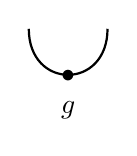
\begin{tikzpicture}
    \begin{knot}
      \strand[thick] (0,0)
        to [out=down,in=down,looseness=2] (1,0);
    \end{knot}
    \node[label=below:{$g$}] at (0.5,-0.6) {$\bullet$};
  \end{tikzpicture}
\] and \[
  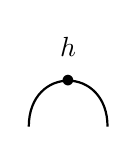
\begin{tikzpicture}
    \begin{knot}
      \strand[thick] (0,0)
        to [out=up,in=up,looseness=2] (1,0);
    \end{knot}
    \node[label=above:{$h$}] at (0.5,0.57) {$\bullet$};
  \end{tikzpicture}
\] respectively. We demand that \[
  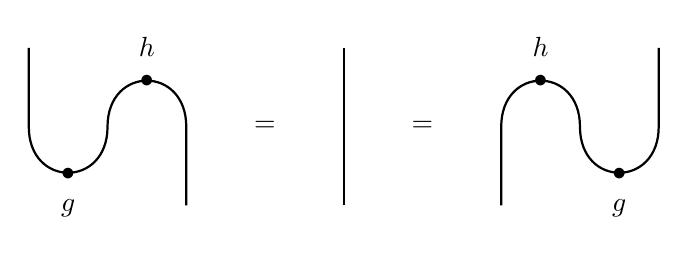
\begin{tikzpicture}
    \begin{scope}[xscale=-1,shift={(-2,0)}]
      \begin{knot}
        \strand[thick] (0,0)
        to (0,1)
        to [out=up,in=up,looseness=2] (1,1)
        to [out=down,in=down,looseness=2] (2,1)
        to (2,2);
      \end{knot}
      \node[label=above:{$h$}] at (0.5,1.57) {$\bullet$};
      \node[label=below:{$g$}] at (1.5,0.4) {$\bullet$};
    \end{scope}
    \node at (3,1) {$=$};
    \begin{scope}[shift={(4,0)}]
      \begin{knot}
        \strand[thick] (0,0) to (0,2);
      \end{knot}
    \end{scope}
    \node at (5,1) {$=$};
    \begin{scope}[shift={(6,0)}]
      \begin{knot}
        \strand[thick] (0,0)
        to (0,1)
        to [out=up,in=up,looseness=2] (1,1)
        to [out=down,in=down,looseness=2] (2,1)
        to (2,2);
      \end{knot}
      \node[label=above:{$h$}] at (0.5,1.57) {$\bullet$};
      \node[label=below:{$g$}] at (1.5,0.4) {$\bullet$};
    \end{scope}
  \end{tikzpicture}
\] which says that the bilinear form \(g\) is nondegenerate. To get
further, we'll also demand that \[
  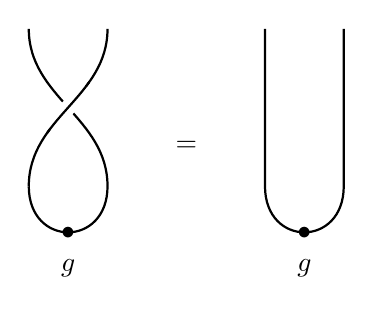
\begin{tikzpicture}
    \begin{knot}[clip width=7]
      \strand[thick] (0,0)
        to [out=down,in=up] (1,-2)
        to [out=down,in=down,looseness=2] (0,-2);
      \strand[thick] (0,-2)
        to [out=up,in=down] (1,0);
      \flipcrossings{1}
    \end{knot}
    \node[label=below:{$g$}] at (0.5,-2.6) {$\bullet$};
    \node at (2,-1.5) {$=$};
    \begin{knot}
      \strand[thick] (3,0)
        to (3,-2)
        to [out=down,in=down,looseness=2] (4,-2)
        to (4,0);
    \end{knot}
    \node[label=below:{$g$}] at (3.5,-2.6) {$\bullet$};
  \end{tikzpicture}
\] This says that the bilinear form \(g\) is symmetric, that is:
\[g(x,y) = g(y,x).\] But we can only state this equation if we're in a
monoidal category where we can ``switch arguments'', which in pictures
goes like this: \[
  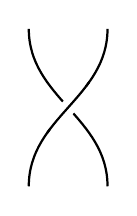
\begin{tikzpicture}
    \begin{knot}[clip width=7]
      \strand[thick] (0,0)
        to [out=down,in=up] (1,-2);
      \strand[thick] (0,-2)
        to [out=up,in=down] (1,0);
      \flipcrossings{1}
    \end{knot}
  \end{tikzpicture}
\] A monoidal category with this feature is called a ``symmetric
monoidal category'' (or more generally a ``braided monoidal category'',
but I don't want to get into those complications here).

So far, so good! The second problem is figuring out how to state the
condition \(|xy| = |x| |y|\). If we translate this into a condition on
our bilinear form \(g\), we get \[g(xy,xy) = g(x,x) g(y,y)\] An algebra
with a nondegenerate bilinear form having this property is called a
``composition algebra''. Hurwitz showed that such an algebra must have
dimension 1, 2, 4, or 8. However, there are examples other than the
famous four, coming from bilinear forms \(g\) that aren't positive
definite. For example, there are the ``split quaternions'' in dimension
4, or the ``split octonions'' in dimension 8.

Now, the problem with the above equational law is that it involves
duplication of arguments. But we can get around this problem by a
standard trick called ``polarization'', which people use a lot in
quantum mechanics.

First let's polarize the argument \(x\). To do this, note that we have
\[
  \begin{aligned}
    g(xy,xy) &= g(x,x) g(y,y)
  \\g(x'y,x'y) &= g(x',x') g(y,y)
  \end{aligned}
\] and also \[g((x+x')y,(x+x')y) = g(x+x',x+x') g(y,y).\] Subtracting
the first two equations from the last and then dividing by \(2\), we get
\[g(xy,x'y) = g(x,x') g(y,y).\] See? We've eliminated the duplication of
the argument \(x\). This new equation obviously implies the original
one.

Next we polarize the argument \(y\). We have \[
  \begin{aligned}
    g(xy,x'y) &= g(x,x') g(y,y)
  \\g(xy',x'y') &= g(x,x') g(y',y')
  \end{aligned}
\] and also \[g(x(y+y'),x'(y+y')) = g(x,x') g(y+y',y+y').\] Subtracting
the first two equations from the last one, we get
\[g(xy,x'y') + g(xy',x'y) = 2 g(x,x') g(y,y')\] Now there is no
duplication of arguments. We've paid a price, though: now our equation
involves addition, so we can only write it down if our category has the
extra feature that we can add morphisms. For this, we want our category
to be ``additive''.

So: the right doctrine in which to define composition algebras is the
doctrine of symmetric monoidal additive categories!

(Technical note: here we want the monoidal and additive structures to
get along nicely: tensoring of morphisms should be bilinear.)

Let me summarize by giving all the details. A ``composition object'' is
an object \(A\) in a symmetric monoidal additive category which is
equipped with morphisms \[
  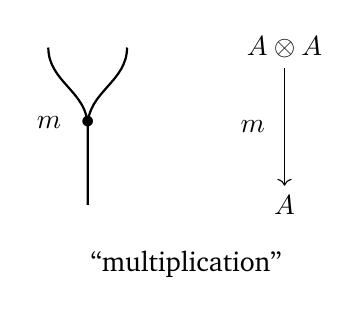
\begin{tikzpicture}
    \begin{knot}
      \strand[thick] (0,0)
        to [out=down,in=up] (0.5,-1)
        to (0.5,-2);
      \strand[thick] (1,0)
        to [out=down,in=up] (0.5,-1);
    \end{knot}
    \node[label=left:{$m$}] at (0.5,-0.95) {$\bullet$};
    \node (s) at (3,0) {$A\otimes A$};
    \node (t) at (3,-2) {$A$};
    \draw[->] (s) to node[label=left:{$m$}]{} (t);
    \node at (1.75,-2.75) {``multiplication''};
  \end{tikzpicture}
\] \[
  \begin{tikzpicture}
    \begin{knot}
      \strand[thick] (0,0)
        to (0,-2);
    \end{knot}
    \node[label=left:{$i$}] at (0,0) {$\bullet$};
    \node (s) at (2,0) {$I$};
    \node (t) at (2,-2) {$A$};
    \draw[->] (s) to node[label=left:{$i$}]{} (t);
    \node at (1,-2.75) {``unit''};
  \end{tikzpicture}
\] \[
  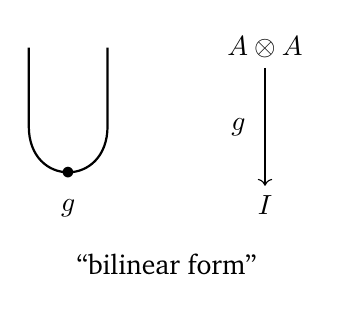
\begin{tikzpicture}
    \begin{knot}
      \strand[thick] (0,0)
        to (0,-1)
        to [out=down,in=down,looseness=2] (1,-1)
        to (1,0);
    \end{knot}
    \node[label=below:{$g$}] at (0.5,-1.6) {$\bullet$};
    \node (s) at (3,0) {$A\otimes A$};
    \node (t) at (3,-2) {$I$};
    \draw[->] (s) to node[label=left:{$g$}]{} (t);
    \node at (1.75,-2.75) {``bilinear form''};
  \end{tikzpicture}
\] \[
  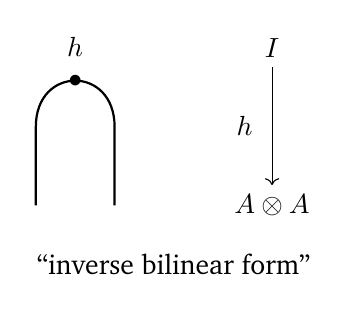
\begin{tikzpicture}
    \begin{knot}
      \strand[thick] (0,-2)
        to (0,-1)
        to [out=up,in=up,looseness=2] (1,-1)
        to (1,-2);
    \end{knot}
    \node[label=above:{$h$}] at (0.5,-0.43) {$\bullet$};
    \node (s) at (3,0) {$I$};
    \node (t) at (3,-2) {$A\otimes A$};
    \draw[->] (s) to node[label=left:{$h$}]{} (t);
    \node at (1.75,-2.75) {``inverse bilinear form''};
  \end{tikzpicture}
\] satisfying the equations already shown: \[
  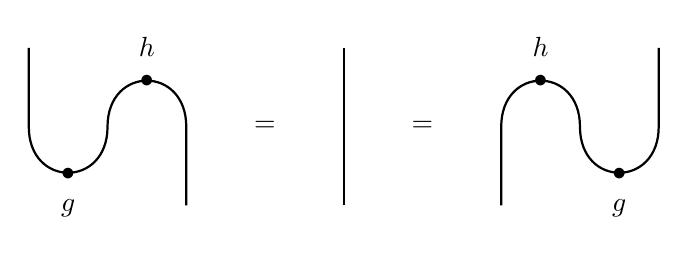
\begin{tikzpicture}
    \begin{scope}[xscale=-1,shift={(-2,0)}]
      \begin{knot}
        \strand[thick] (0,0)
        to (0,1)
        to [out=up,in=up,looseness=2] (1,1)
        to [out=down,in=down,looseness=2] (2,1)
        to (2,2);
      \end{knot}
      \node[label=above:{$h$}] at (0.5,1.57) {$\bullet$};
      \node[label=below:{$g$}] at (1.5,0.4) {$\bullet$};
    \end{scope}
    \node at (3,1) {$=$};
    \begin{scope}[shift={(4,0)}]
      \begin{knot}
        \strand[thick] (0,0) to (0,2);
      \end{knot}
    \end{scope}
    \node at (5,1) {$=$};
    \begin{scope}[shift={(6,0)}]
      \begin{knot}
        \strand[thick] (0,0)
        to (0,1)
        to [out=up,in=up,looseness=2] (1,1)
        to [out=down,in=down,looseness=2] (2,1)
        to (2,2);
      \end{knot}
      \node[label=above:{$h$}] at (0.5,1.57) {$\bullet$};
      \node[label=below:{$g$}] at (1.5,0.4) {$\bullet$};
    \end{scope}
  \end{tikzpicture}
\] and \[
  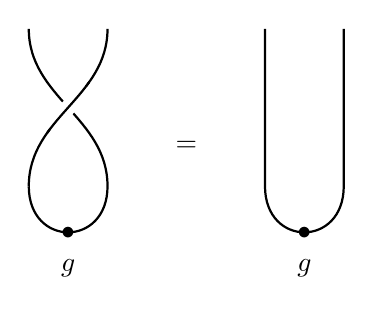
\begin{tikzpicture}
    \begin{knot}[clip width=7]
      \strand[thick] (0,0)
        to [out=down,in=up] (1,-2)
        to [out=down,in=down,looseness=2] (0,-2);
      \strand[thick] (0,-2)
        to [out=up,in=down] (1,0);
      \flipcrossings{1}
    \end{knot}
    \node[label=below:{$g$}] at (0.5,-2.6) {$\bullet$};
    \node at (2,-1.5) {$=$};
    \begin{knot}
      \strand[thick] (3,0)
        to (3,-2)
        to [out=down,in=down,looseness=2] (4,-2)
        to (4,0);
    \end{knot}
    \node[label=below:{$g$}] at (3.5,-2.6) {$\bullet$};
  \end{tikzpicture}
\] together with the left and right unit laws: \[
  \begin{tikzpicture}
    \begin{knot}
      \strand[thick] (0,0.5) to (0,0);
      \strand[thick] (1,1.5) to (1,0);
      \strand[thick] (0,0)
        to [out=down,in=up] (0.5,-1)
        to (0.5,-2);
      \strand[thick] (1,0)
        to [out=down,in=up] (0.5,-1);
    \end{knot}
    \node[label=left:{$i$}] at (0,0.5) {$\bullet$};
    \node[label=left:{$m$}] at (0.5,-0.95) {$\bullet$};
    \node at (2,-0.25) {$=$};
    \begin{knot}
      \strand[thick] (3,1.5) to (3,-2);
    \end{knot}
    \node at (4,-0.25) {$=$};
    \begin{scope}[xscale=-1,shift={(-6,0)}]
      \begin{knot}
        \strand[thick] (0,0.5) to (0,0);
        \strand[thick] (1,1.5) to (1,0);
        \strand[thick] (0,0)
          to [out=down,in=up] (0.5,-1)
          to (0.5,-2);
        \strand[thick] (1,0)
          to [out=down,in=up] (0.5,-1);
      \end{knot}
      \node[label=right:{$i$}] at (0,0.5) {$\bullet$};
      \node[label=left:{$m$}] at (0.5,-0.95) {$\bullet$};
    \end{scope}
  \end{tikzpicture}
\] and best of all, the equation
\[g(xy,x'y') + g(xy',x'y) = 2 g(x,x') g(y,y')\] translated into pictures
like this: \[
  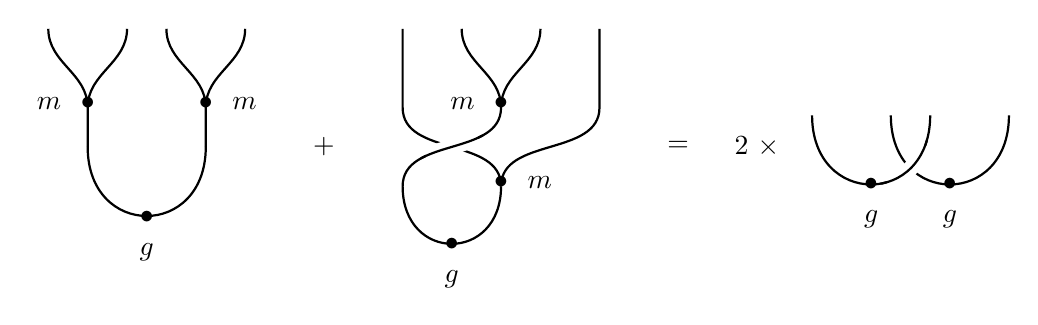
\begin{tikzpicture}
    \begin{knot}
      \strand[thick] (0,0)
        to [out=down,in=up] (0.5,-1)
        to (0.5,-1.5);
      \strand[thick] (1,0)
        to [out=down,in=up] (0.5,-1);
      \strand[thick] (1.5,0)
        to [out=down,in=up] (2,-1)
        to (2,-1.5);
      \strand[thick] (2.5,0)
        to [out=down,in=up] (2,-1);
      \strand[thick] (0.5,-1.5)
        to [out=down,in=down,looseness=2] (2,-1.5);
    \end{knot}
    \node[label=left:{$m$}] at (0.5,-0.95) {$\bullet$};
    \node[label=right:{$m$}] at (2,-0.95) {$\bullet$};
    \node[label=below:{$g$}] at (1.25,-2.4) {$\bullet$};
    \node at (3.5,-1.5) {$+$};
    \begin{scope}[shift={(4.5,0)}]
      \begin{knot}[clip width=7]
        \strand[thick] (0,0)
          to (0,-1)
          to [out=down,in=up] (1.25,-2);
        \strand[thick] (0.75,0)
          to [out=down,in=up] (1.25,-1)
          to [out=down,in=up] (0,-2)
          to [out=down,in=down,looseness=2] (1.25,-2);
        \strand[thick] (1.75,0)
          to [out=down,in=up] (1.25,-1);
        \strand[thick] (2.5,0) to (2.5,-1)
          to [out=down,in=up] (1.25,-2);
        \flipcrossings{1}
      \end{knot}
      \node[label=left:{$m$}] at (1.25,-0.95) {$\bullet$};
      \node[label=right:{$m$}] at (1.25,-1.95) {$\bullet$};
      \node[label=below:{$g$}] at (0.625,-2.74) {$\bullet$};
    \end{scope}
    \node at (8,-1.5) {$=$};
    \node at (9,-1.5) {$2\,\,\times$};
    \begin{scope}[shift={(9.7,-1.1)}]
      \begin{knot}[clip width=7]
        \strand[thick] (0,0)
          to [out=down,in=down,looseness=2] (1.5,0);
        \strand[thick] (1,0)
          to [out=down,in=down,looseness=2] (2.5,0);
      \end{knot}
      \node [label=below:{$g$}] at (0.75,-0.88) {$\bullet$};
      \node [label=below:{$g$}] at (1.75,-0.88) {$\bullet$};
    \end{scope}
  \end{tikzpicture}
\]

Now, given all this stuff, we can define the ``dimension'' of our
composition algebra to be the value of this morphism from \(I\) to
\(I\): \[
  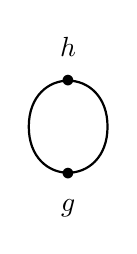
\begin{tikzpicture}
    \begin{knot}
      \strand[thick] (0,0)
        to [out=up,in=up,looseness=2] (1,0)
        to [out=down,in=down,looseness=2] (0,0);
    \end{knot}
    \node[label=above:{$h$}] at (0.5,0.57) {$\bullet$};
    \node[label=below:{$g$}] at (0.5,-0.6) {$\bullet$};
  \end{tikzpicture}
\] This reduces to the usual dimension of the algebra \(A\) when we're
in the category \(\mathsf{Vect}\). Of course, only in certain categories
is this dimension bound to be a \emph{number} --- namely, those
categories where every morphism from \(I\) to \(I\) is some number times
the identity morphism.

By making an extra assumption like this, Boos is able to give a
``picture proof'' that in a large class of symmetric monoidal additive
categories, every composition object has dimension 1, 2, 4 or 8. This is
great, because it means we can talk about things like real, complex,
quaternionic and octonionic objects in a wide variety of categories! He
doesn't prove such objects exist, but I think this should be easy, at
least with some extra assumptions which would allow us to construct them
``by hand'', mimicking standard constructions of the normed division
algebras.

But now I must warn you of some things. Boos doesn't state his result
the way I would! Instead of working with ``composition objects'' (which
appear to be my own invention), he works with ``vector product
algebras''. These are modelled, not after the normed division algebras
themselves, but after their ``imaginary parts''. These have both an
inner product and a ``vector product''.

For example, the imaginary quaternions form a 3-dimensional vector
product algebra with vector product given by
\[a\times b = \frac12(ab - ba).\] This is just the usual cross product!
The same formula makes the imaginary octonions into a 7-dimensional
vector product algebra, the imaginary complex numbers into a boring
1-dimensional one\ldots{} and the imaginary real numbers into an even
more boring 0-dimensional one.

Boos writes down the axioms for a vector product algebra using pictures
much like I just did for a composition object, and he shows that under
some pretty mild conditions you can freely go back and forth between the
two concepts.

I think you can summarize his theorem on vector product algebras as
follows: in all symmetric monoidal \(R\)-linear categories where \(R\)
is a commutative ring containing \(\mathbb{Z}[\frac12]\) and \(I\) is a
simple object, vector product algebras must have dimension 0, 1, 3, or
7. He doesn't state his result quite this way, but I'm pretty sure
that's what it boils down to. As for the jargon: a category is
``\(R\)-linear'' if the homsets are \(R\)-modules and composition of
morphisms is bilinear; for monoidal categories we also want tensoring
morphisms to be bilinear. The ring \(\mathbb{Z}[\frac12]\) consists of
all fractions with a power of 2 in the denominator --- Boos needs this
because he needs to divide by \(2\) at some point in his argument. For
an \(R\)-linear category, an object \(I\) is ``simple'' if
\(\operatorname{Hom}(I,I) = R\). This allows us to interpret the
dimension of our vector product algebra as an element of \(R\) --- which
Boos shows is actually one of the integers 0, 1, 3, or 7.

Let me conclude by showing you Boos' main axiom for vector product
algebras, written in terms of pictures: \[
  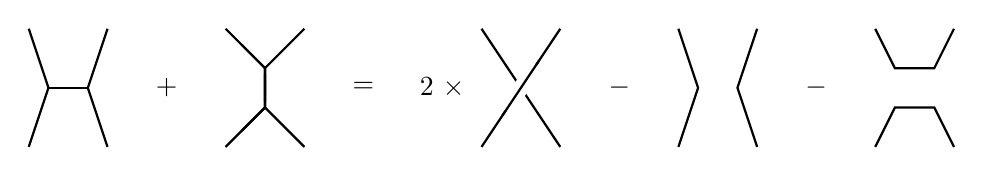
\begin{tikzpicture}
    \begin{knot}[clip width=0]
      \strand[thick] (0,0)
        to (0.25,-0.75)
        to (0,-1.5);
      \strand[thick] (1,0)
        to (0.75,-0.75)
        to (1,-1.5);
      \strand[thick] (0.25,-0.75) to (0.75,-0.75);
    \end{knot}
    \node at (1.75,-0.75) {$+$};
    \begin{scope}[shift={(2.5,0)}]
      \begin{knot}[clip width=0]
        \strand[thick] (0,0)
          to (0.5,-0.5)
          to (0.5,-1)
          to (0,-1.5);
        \strand[thick] (1,0)
          to (0.5,-0.5)
          to (0.5,-1)
          to (1,-1.5);
      \end{knot}
    \end{scope}
    \node at (4.25,-0.75) {$=$};
    \node at (5.25,-0.75) {$2\,\,\times$};
    \begin{scope}[shift={(5.75,0)}]
      \begin{knot}[clip width=7]
        \strand[thick] (0,0) to (1,-1.5);
        \strand[thick] (1,0) to (0,-1.5);
        \flipcrossings{1}
      \end{knot}
    \end{scope}
    \node at (7.5,-0.75) {$-$};
    \begin{scope}[shift={(8.25,0)}]
      \begin{knot}
        \strand[thick] (0,0)
          to (0.25,-0.75)
          to (0,-1.5);
        \strand[thick] (1,0)
          to (0.75,-0.75)
          to (1,-1.5);
      \end{knot}
    \end{scope}
    \node at (10,-0.75) {$-$};
    \begin{scope}[shift={(10.75,0)}]
      \begin{knot}
        \strand[thick] (0,0)
          to (0.25,-0.5)
          to (0.75,-0.5)
          to (1,0);
        \strand[thick] (0,-1.5)
          to (0.25,-1)
          to (0.75,-1)
          to (1,-1.5);
      \end{knot}
    \end{scope}
  \end{tikzpicture}
\] Ain't it cool? Fans of knot theory will be struck by the resemblance
to various ``skein relations''. Fans of physics will be reminded of
Feynman diagrams. But what is the secret inner meaning?

\begin{center}\rule{0.5\linewidth}{0.5pt}\end{center}

\emph{``The perplexity of life arises from there being too many
interesting things in it for us to be interested properly in any of
them.''} --- G. K. Chesterton, 1909
\hypertarget{week170}{%
\section{DATE}\label{week170}}

I've been travelling around a lot lately. For a couple of weeks I was in
Turkey, resisting the lure of the many internet cafes. I urge you all to
visit Istanbul when you get a chance! Fascinating music fills the
streets. There are a lot of nice bookstore-cafes on Istiklal Caddesi
near Taksim Square, and a huge number of musical instrument shops at the
other end of this street, down near Tunel Square. I bought a nice
doumbek at one of these shops, and looked at lots of ouzes, sazes and
neys, none of which I can play. It's also imperative to check out the
Grand Bazaar, the mosques, and the Topkapi Palace --- the harem there
has most beautiful geometric tiling patterns I've ever seen. I'm not
sure why that's true; perhaps this is where the sultans spent most of
their time.

The mathematics of tilings is a fascinating subject, but that's not what
I'm going to talk about. After my trip to Turkey, I went to a conference
at Stanford:

\begin{enumerate}
\def\labelenumi{\arabic{enumi})}
\tightlist
\item
  Conference on Algebraic Topological Methods in Computer Science,
  Stanford University, \texttt{http://math.stanford.edu/atmcs/index.htm}
\end{enumerate}

There were lots of fun talks, but I'll just mention two.

The talk most related to physics was the one by my friend Dan
Christensen, who spoke on ``Spin Networks, Spin Foams and Quantum
Gravity'', describing a paper he is writing with Greg Egan on efficient
algorithms for computing Riemannian \(10j\) symbols. Dan is a homotopy
theorist at the University of Western Ontario, and Greg is my favorite
science fiction writer. They're both interested in quantum gravity, and
they're both good at programming. Together with some undergraduate
students of Dan's, the three of us are starting to study the Riemannian
and Lorentzian Barrett-Crane models of quantum gravity with the help of
computer simulations. But to get anywhere with this, we need to get good
at computing ``\(10j\) symbols''.

Huh? ``\(10j\) symbols''??

Well, as with any quantum field theory, the key to the Barrett-Crane
model is the partition function. In the Riemannian version of this
theory, you compute the partition function as follows. First you take
your 4-dimensional manifold representing spacetime and triangulate it.
Then you label all the triangles by spins
\(j = 0, 1/2, 1, 3/2, \ldots\). Following certain specific formulas you
then calculate a number for each 4-simplex, a number for each
tetrahedron, and a number for each triangle, using the spin labellings.
Then you multiply all these together. Finally you sum over all
labellings to get the partition function. The only tricky part is the
convergence of this sum, which was proved by Perez:

\begin{enumerate}
\def\labelenumi{\arabic{enumi})}
\setcounter{enumi}{1}
\tightlist
\item
  Alejandro Perez, ``Finiteness of a spin foam model for euclidean
  quantum general relativity'', \emph{Nucl. Phys.} \textbf{B599} (2001)
  427--434. Also available as
  \href{https://arxiv.org/abs/gr-qc/0011058}{\texttt{gr-qc/0011058}}.
\end{enumerate}

The most interesting aspect of all this is the formula giving numbers
for 4-simplices. A 4-simplex has 10 triangular faces all of which get
labelled by spins, and the formula says how to compute a number from
these 10 spins --- the so-called ``\(10j\) symbol''.

How do you compute \(10j\) symbols? One approach involves representation
theory, or in lowbrow terms, multiplying a bunch of matrices.
Unfortunately, if you go about this in the most simple-minded obvious
fashion, when the spins labelling your triangles are all about equal to
\(j\), you wind up needing to work with matrices that are as big as
\(N\times N\), where \[N = (2j+1)^{12}.\] If you do this, already for
\(j = 1/2\) you are dealing with square matrices that are \(2^{12}\) by
\(2^{12}\). This is too big to be practical!

In computer science lingo, this algorithm sucks because it uses
\(\mathcal{O}(j^{12})\) time and also \(\mathcal{O}(j^{12})\) space. You
might think it was \(\mathcal{O}(j^{24})\), but it's not that
bad\ldots{} however, it's still very bad!

Luckily, Dan and Greg have figured out a much more efficient algorithm,
which uses only \(\mathcal{O}(j^6)\) time and \(\mathcal{O}(j)\) space.
Alternatively, with more caching of data, they can get
\(\mathcal{O}(j^5)\) time and \(\mathcal{O}(j^3)\) space, or maybe even
better. Using an algorithm of this sort, Dan can compute the \(10j\)
symbol for spins up to 55. For all spins equal to 55, the calculation
took about 10 hours on a normal desktop computer. However, for computing
partition functions it appears that small spins are much more important,
and then the computation takes milliseconds.

(Actually, for computing partition functions, Dan is not using a
desktop: he is using a Beowulf cluster, which is a kind of supercomputer
built out of lots of PCs. This works well for partition functions
because the computation is highly parallelizable.)

John Barrett has also figured out a very different approach to computing
\(10j\) symbols:

\begin{enumerate}
\def\labelenumi{\arabic{enumi})}
\setcounter{enumi}{2}
\tightlist
\item
  John W. Barrett, ``The classical evaluation of relativistic spin
  networks'', \emph{Adv. Theor. Math. Phys.} \textbf{2} (1998),
  593--600. Also available as
  \href{https://arxiv.org/abs/math.QA/9803063}{\texttt{math.QA/9803063}}.
\end{enumerate}

In this approach one computes the \(10j\) symbols by doing an integral
over the space of geometries of a 4-simplex --- or more precisely, over
a product of 5 copies of the 3-sphere, where a point on one of these
3-spheres describes the normal vector to one of the 5 tetrahedral faces
of the 4-simplex.

Dan and Greg have also written programs that calculate the \(10j\)
symbols by doing these integrals. The answers agree with their other
approach.

We've already been getting some new physical insights from these
calculations. If you write down the integral formula for the Riemannian
\(10j\) symbols, a stationary phase argument due to John Barrett and
Ruth Williams suggests that, at least in the limit of large spins, the
dominant contribution to the integral for the \(10j\) symbol comes from
4-simplices whose face areas are the 10 spins in your \(10j\) symbols:

\begin{enumerate}
\def\labelenumi{\arabic{enumi})}
\setcounter{enumi}{3}
\tightlist
\item
  John W. Barrett and Ruth M. Williams, ``The asymptotics of an
  amplitude for the 4-simplex'', \emph{Adv. Theor. Math. Phys.}
  \textbf{3} (1999), 209--215. Also available as
  \href{https://arxiv.org/abs/gr-qc/9809032}{\texttt{gr-qc/9809032}}.
\end{enumerate}

However, Dan and Greg's calculations suggest instead that the dominant
contribution comes from certain ``degenerate'' configurations. Some of
these correspond to points on the product of 5 copies of the 3-sphere
that are close to points of the form \((v,v,v,v,v)\) --- or roughly
speaking, 4-simplices whose 5 normal vectors are all pointing the same
way. Others come from sprinkling minus signs in this list of vectors.
Heuristically, we can think of these degenerate configurations as
extremely flattened-out 4-simplices.

For simplicity, we have concentrated so far on studying the \(10j\)
symbols in the case when all 10 spins are equal. In this case we can
show that the only nondegenerate 4-simplex with these spins as face
areas is the regular 4-simplex (all of whose faces are congruent
equilateral triangles). Greg used stationary phase to compute the
contribution of this regular 4-simplex to Barrett's integral formula for
the \(10j\) symbols, and it turned out that asymptotically, for large
\(j\), this contribution decays like \(j^{-9/2}\). On the other hand,
Dan's numerical computations of the \(10j\) symbol suggests that it goes
like \(j^{-2}\). This suggests that for large \(j\), the contribution of
the regular 4-simplex is dwarfed by that of the degenerate 4-simplices.

Greg has gotten more evidence for this by studying the integral formula
for the \(10j\) symbols and estimating the contribution due to
degenerate 4-simplices. This estimate indeed goes like \(j^{-2}\) for
large \(j\).

There is a lot more to be understood here, but plunging ahead
recklessly, we can ask what all this means for the physics of the
Barrett-Crane model. For example: is the dominant contribution to the
partition function going to come from spacetime geometries with lots of
degenerate 4-simplices?

I think that's a premature conclusion, because we already have evidence
that 4 -simplices with large face areas are not contributing that much
compared to those with small face areas when we compute the partition
function as a sum over spin foams. In other words, it seems that in the
Riemannian Barrett-Crane model, spacetime is mostly made of lots of
small 4-simplices, rather than a few giant ones. If so, the tendency for
the giant ones to flatten out may not be so bad.

Of course the really important thing will be to study these questions
for the Lorentzian theory, but it's good to look at the Riemannian
theory too.

Another talk on a subject close to my heart was given by Noson Yanofsky.
It was based on these papers of his, especially the last:

\begin{enumerate}
\def\labelenumi{\arabic{enumi})}
\setcounter{enumi}{4}
\item
  Noson S. Yanofsky, ``Obstructions to coherence: natural noncoherent
  associativity'', \emph{Jour. Pure Appl. Alg.} \textbf{147} (2000),
  175--213. Also available at
  \href{https://arxiv.org/abs/math.QA/9804106}{\texttt{math.QA/9804106}}.

  ``The syntax of coherence''. To appear in \emph{Cahiers Top. Geom.
  Diff.}. Also available at
  \href{https://arxiv.org/abs/math.CT/9910006}{\texttt{math.CT/9910006}}.

  ``Coherence, homotopy and 2-theories''. To appear in \emph{K-Theory}.
  Also available at
  \href{https://arxiv.org/abs/math.CT/0007033}{\texttt{math.CT/0007033}}.
\end{enumerate}

One of the cool things Yanofsky has done is to study what happens when
we categorify Lawvere's concept of an ``algebraic theory''. I've already
explained this idea of ``algebraic theory'' in
\protect\hyperlink{week53}{``Week 53''} and
\protect\hyperlink{week136}{``Week 136''}, so I'll just quickly recap it
here:

The notion of ``algebraic theory'' is just a slick way to study sets
equipped with extra algebraic structure. We call a category
\(\mathcal{C}\) with finite products an ``algebraic theory'' if its
objects are all of the form \(1, X, X^2, X^3, \ldots\) for some
particular object \(X\). We call a product-preserving functor
\(F\colon\mathcal{C}\to\mathsf{Set}\) a ``model'' of the theory. And we
call a natural transformation between such functors a ``homomorphism''
between models. This gives us a category \(\mathsf{Mod}(\mathcal{C})\)
consisting of models and homomorphisms between them, and it turns out
that many categories of algebraic gadgets are of this form: the category
of monoids, the category of groups, the category of abelian groups, and
so on.

Since algebraic theories are good for studying sets with extra algebraic
structure, we might hope that by categorifying, we could obtain a
concept of ``algebraic 2-theories'' which is good for studying
\emph{categories} with extra algebraic structure. And it's true! In
1974, John Gray defined an ``algebraic 2-theory'' to be a 2-category
\(\mathcal{C}\) with finite products, all of whose objects are of the
form \(1, X, X^2, X^3,\ldots\) for some particular object \(X\). Define
a ``model'' of this 2-theory to be a product-preserving 2-functor
\(F\colon\mathcal{C}\to\mathsf{Cat}\). And define a ``homomorphism''
between models to be a pseudonatural transformation between such
2-functors.

Huh? ``Pseudonatural''??

Sorry, now things are getting a bit technical: the right thing going
between 2-functors is not a natural transformation but something a bit
weaker called a ``pseudonatural transformation'', where the usual
commuting squares in the definition of a natural transformation are
required to commute only up to certain specified 2-isomorphisms, which
in turn satisfy some coherence laws described here:

\begin{enumerate}
\def\labelenumi{\arabic{enumi})}
\setcounter{enumi}{5}
\tightlist
\item
  G. Maxwell Kelly and Ross Street, \emph{Review of the elements of
  2-categories}, Springer Lecture Notes in Mathematics \textbf{420},
  Berlin, 1974, pp.~75--103.
\end{enumerate}

However, you don't need to understand the details right now. There is
also something going between pseudonatural transformations called a
``modification'', and this gives us ``2-homomorphisms'' between
homomorphisms between models of our algebraic theory. Thanks to these
there is a 2-category \(\mathsf{Mod}(\mathcal{C})\) consisting of models
of our 2-theory homomorphisms between those, and 2-homomorphisms between
those.

Some examples might help! For example, there's a 2-theory
\(\mathcal{C}\) called the ``theory of weak monoidal categories''.
Models of \(\mathcal{C}\) are weak monoidal categories, homomorphisms
are monoidal functors, and 2-homomorphisms are natural transformations,
so \(\mathsf{Mod}(\mathcal{C})\) is the usual 2-category of monoidal
2-categories. There's a similar 2-theory \(\mathcal{C}'\) called ``the
theory of strict monoidal categories'', for which
\(\mathsf{Mod}(\mathcal{C}')\) is the usual 2-category of strict
monoidal categories.

(Hyper-technical note for \(n\)-category mavens only: in both examples
here, monoidal functors are required to preserve unit and tensor product
only \emph{up to coherent natural isomorphism}. This nuance is what we
get from working with pseudonatural rather than natural transformations.
Without this nuance, some of the stuff I'm about to say would be false.)

Now, whenever we have a product-preserving 2-functor between 2-theories,
say \(F\colon\mathcal{C}\to\mathcal{C}'\), we get an induced 2-functor
going the other way,
\[F^*\colon\mathsf{Mod}(\mathcal{C}')\to\mathsf{Mod}(\mathcal{C}).\] For
example, there's a product-preserving 2-functor from the theory of weak
monoidal categories to the theory of strict monoidal categories, and
this lets us turn any strict monoidal category into a weak one.

Now in this particular example, \(F^*\) is a biequivalence, which is the
nice way to say that the 2-categories \(\mathsf{Mod}(C)\) and
\(\mathsf{Mod}(C')\) are ``the same'' for all practical purposes. And in
fact, saying that this particular \(F^*\) is a biequivalence is really
just an ultra-slick version of Mac Lane's theorem --- the theorem we use
to turn weak monoidal categories into strict ones.

Now, Mac Lane's theorem is the primordial example of a ``strictification
theorem'' --- a theorem that lets us turn ``weak'' algebraic structures
on categories into ``strict'' ones, where lots of isomorphisms, like the
associators in the monoidal category example, are assumed to be
equations. This suggests that lots of coherence theorems can be stated
by saying that 2-functors of the form \(F^*\) are biequivalences.

So: is there a super-general strictification theorem where we can start
from any 2-theory \(\mathcal{C}\) and get a ``strictified'' version
\(\mathcal{C}'\) together with an \(F\colon\mathcal{C}\to\mathcal{C}'\)
such that \(F^*\) is a biequivalence?

As a step in this direction, Yanofsky has cooked up a model category of
algebraic 2-theories, in which \(F\colon\mathcal{C}\to\mathcal{C}'\) is
a weak equivalence precisely when \(F^*\) is a biequivalence.

Huh? ``Model category''??

Well, if you don't know what a ``model category'' is, you're in serious
trouble now! They're a concept invented by Quillen for generalizing the
heck out of homotopy theory. Try reading his book:

\begin{enumerate}
\def\labelenumi{\arabic{enumi})}
\setcounter{enumi}{6}
\tightlist
\item
  Daniel G. Quillen, \emph{Homotopical Algebra}, Springer Lecture Notes
  in Mathematics, vol.~\textbf{43}, Springer, Berlin, 1967.
\end{enumerate}

or for something newer:

\begin{enumerate}
\def\labelenumi{\arabic{enumi})}
\setcounter{enumi}{7}
\tightlist
\item
  Mark Hovey, \emph{Model Categories}, American Mathematical Society
  Mathematical Surveys and Monographs, vol \textbf{63}, Providence,
  Rhode Island, 1999.
\end{enumerate}

or else:

\begin{enumerate}
\def\labelenumi{\arabic{enumi})}
\setcounter{enumi}{8}
\tightlist
\item
  Paul G. Goerss and John F. Jardine, \emph{Simplicial Homotopy Theory},
  Birkhauser, Boston, 1999.
\end{enumerate}

(By the way, Jardine was one of the organizers of this Stanford
conference, along with Gunnar Carlsson. He told me he had created a
hypertext version of this book, but has not been able to get the
publisher interested in it. Sad!)

Anyway, in the framework of model categories, the problem of
``strictifying'' an algebraic structure on categories then amounts to
finding a ``minimal model'' of a given 2-theory \(\mathcal{C}\) ---
roughly speaking, a weakly equivalent 2-theory with as little flab as
possible. The concept of ``minimal model'' is important in homotopy
theory, but apparently Yanofsky is the first to have given a general
definition of this concept applicable to any model category. Yanofsky
has not shown that every algebraic 2-theory admits a minimal model, but
this seems like a fun and interesting question.

\begin{center}\rule{0.5\linewidth}{0.5pt}\end{center}

\emph{all ignorance toboggans into know and trudges up to ignorance
again.} --- e.e.cummings, 1959
\hypertarget{week171}{%
\section{DATE}\label{week171}}

There isn't a Nobel prize for mathematics. You've probably heard why:
Alfred Nobel was annoyed that the famous mathematician Mittag-Leffler
had an affair with his wife. Well, that's what they say, anyway. It
makes a great story. The only problem is, Nobel was never married! So
it's just another urban legend. For more details, see:

\begin{enumerate}
\def\labelenumi{\arabic{enumi})}
\tightlist
\item
  Urban legends reference pages, ``The Prize's Rite'',
  \texttt{http://www.snopes2.com/science/nobel.htm}
\end{enumerate}

More likely, Nobel just didn't consider mathematics sufficiently
practical. In any event, mathematicians have always felt a bit grumpy
about this slight. Their adoption of the Fields Medal as a kind of
substitute has never been completely satisfying. For one thing, the
Fields Medal is only for work done before the age of 40 --- a condition
that seems ever more silly with the wisdom of age. For another, the
Fields prize gives you a measly 15,000 Canadian dollars, while the Nobel
prize keeps going up: this year, it was 10 million Swedish crowns, or
almost a million bucks.

Anyway, now there may be a better substitute: the Abel Prize.

\begin{itemize}
\tightlist
\item
  ``Norway Establishes Abel Prize in Mathematics'',
  \texttt{http://www.maa.org/news/abel\_prize.html}
\end{itemize}

It even almost rhymes with Nobel! Abel, of course, was a famous
Norwegian mathematician, and this prize will be awarded annually by the
government of Norway, starting in 2003. It will have a value of about
\$500,000, at least initially. Even better, it will be awarded on a
first-come, first-serve basis\ldots{} so send in your application now.

When I was in Cambridge this summer, I visited Tom Leinster and Eugenia
Cheng, who showed me around the new mathematics buildings. The Cambridge
system is too Byzantine for a mere American to understand, but there are
two main things resembling a ``mathematics department'': DPMSS, the
Department of Pure Mathematics and Mathematical Statistics, and DAMTP,
the Department of Applied Mathematics and Theoretical Physics. They used
to be in separate dilapidated buildings downtown on Silver Street, but
now they occupy two towers in a huge complex near the Newton Institute,
on the outskirts of town.

The new setup is pretty cool. Parts of it are still under construction,
but you can get the idea already. Different breeds of mathematicians
will be housed in different towers, all surrounding a central building
resembling an airplane hanger, which is actually an enormous cafeteria.
The univeral human interest in food will lure otherwise aloof
specialists to mingle and chat. I even saw Hawking there one day.
However, there is also a separate coffee lounge at the base of each
tower, so the different groups can have slightly more private chats.
Futuristic light sensors lower curtains in the cafeteria whenever the
sun comes out, to enhance the visitor's impression that it's always
cloudy in England. But the really cool thing is that every tower has a
door on the second floor which opens out to the \emph{roof} of the
cafeteria. The roof is covered with grass, like a little park! Finally,
people working on fluid dynamics are kept in the basement, which gurgles
mysteriously with the sound of experiments.

Leinster and Cheng are both students of Martin Hyland, and they both
work on \(n\)-categories. I've talked about their work before in
\protect\hyperlink{week165}{``Week 165''}. Leinster has just come out
with a nice paper on \(n\)-categories:

\begin{enumerate}
\def\labelenumi{\arabic{enumi})}
\tightlist
\item
  Tom Leinster, ``A survey of definitions of \(n\)-category'', available
  at
  \href{https://arxiv.org/abs/math.CT/0107188}{\texttt{math.CT/0107188}}.
\end{enumerate}

By now, there are lots of definitions of ``weak \(n\)-category'', and
our job is to understand how they're related. This paper is required
reading for anyone interested in this business: it goes through 10
different definitions, giving each definition in two pages and then
using two more pages to show how it works for \(n\) less than or equal
to 2. It also has a nice annotated bibliography giving some of the
history of the subject.

While I'm talking about review articles, here are some review articles
on quantum gravity:

\begin{enumerate}
\def\labelenumi{\arabic{enumi})}
\setcounter{enumi}{1}
\tightlist
\item
  Steve Carlip, ``Quantum gravity: a progress report'', \emph{Rep.~Prog.
  Phys.} \textbf{64} (2001) 885--942, also available at
  \href{https://arxiv.org/abs/gr-qc/0108040}{\texttt{gr-qc/0108040}}.
\end{enumerate}

This is an excellent \emph{long} description of where we stand on
quantum gravity, with a strong focus on the big conceptual problems.
Again, it's required reading for anyone in this field. It doesn't do
justice to string theory, which is a mammoth subject in its own. For
that, you might try this article which I bumped into in the same
journal:

\begin{enumerate}
\def\labelenumi{\arabic{enumi})}
\setcounter{enumi}{2}
\tightlist
\item
  Ulf Daniellson, ``Introduction to string theory'', \emph{Rep.~Prog.
  Phys.} \textbf{64} (2001) 51-96.
\end{enumerate}

It seems to do a pretty good job of the impossible --- explaining all of
string theory in less than 50 pages. Of course, if you want to get
serious, you'll eventually have to read some of the string theory
textbooks listed in \protect\hyperlink{week124}{``Week 124''} and
elsewhere.

There is also a new introduction to loop quantum gravity available
online. It's more of a book than an article:

\begin{enumerate}
\def\labelenumi{\arabic{enumi})}
\setcounter{enumi}{3}
\tightlist
\item
  Thomas Thiemann, \emph{Introduction to modern canonical quantum
  general relativity}, 301 pages, available at
  \href{https://arxiv.org/abs/gr-qc/0110034}{\texttt{gr-qc/0110034}}.
\end{enumerate}

This is really \emph{the} place to go if you want to catch up on the
last 15 years of work on loop quantum gravity. It's truly impressive.
It'll make fairly substantial demands on the average physicist's
mathematical know-how: for example, not just differential geometry,
which everyone into gravity must know, but also functional analysis.
Luckily, it has an appendix over 40 pages long which explains much of
the needed math. For the would-be grad student or postdoc, a very
helpful feature is the list of institutions where loop quantum gravity
is studied, in the Introduction.

Speaking of loop quantum gravity, here are a few interesting new papers
on that subject:

\begin{enumerate}
\def\labelenumi{\arabic{enumi})}
\setcounter{enumi}{4}
\item
  Rodolfo Gambini and Jorge Pullin, ``Consistent discretizations for
  classical and quantum general relativity'', available as
  \href{https://arxiv.org/abs/gr-qc/0108062}{\texttt{gr-qc/0108062}}.
\item
  Luca Bombelli, ``Statistical geometry of random weave states'',
  available as
  \href{https://arxiv.org/abs/gr-qc/0101080}{\texttt{gr-qc/0101080}}.
\item
  Michael Seifert, ``Angle and volume studies in quantized space'', 85
  pages, available as
  \href{https://arxiv.org/abs/gr-qc/0108047}{\texttt{gr-qc/0108047}}.
\end{enumerate}

The paper by Gambini and Pullin argues that good spin foam models will
come from quantizing ``consistent'' discretizations of general
relativity, that is, those where the discretized equations of motion
preserve the constraints on initial data, and where the solutions
converge to solutions of the continuum equations in the limit where the
discretization is made ever more fine.

The paper by Bombelli presents a proposal for states of loop quantum
gravity that should be good approximations to classical geometries. The
idea is to take a Riemannian manifold, sprinkle points on it randomly
form the corresponding Voronoi diagram, and label the edges with spins
in a certain way to get a spin network. If we then average over all
possible ways of randomly sprinkling these points, we get Bombelli's
``random weave state'' --- a kinematical state of quantum gravity that
approximates of the Riemannian geometry we started with.

I don't know if that made sense to you. Do you at least know what a
Voronoi diagram is? To explain that, a picture is worth a thousand
words, so I won't explain the concept --- I'll just urge you to play
with this applet:

\begin{enumerate}
\def\labelenumi{\arabic{enumi})}
\setcounter{enumi}{8}
\tightlist
\item
  Paul Chew, Voronoi/Delaunay Applet,
  \texttt{http://www.cs.cornell.edu/Info/People/chew/Delaunay.html}
\end{enumerate}

If you click the mouse to sprinkle the rectangle with points, you'll see
a bunch of edges appear, which intersect in vertices, forming a graph
called the Voronoi diagram. By epxerimenting a bit you can figure out
how it works --- or else you can cheat and read the text. You'll see
that generically the vertices of this graph are trivalent: they have
three edges coming out of them. If you click on the button that says
``Delaunay Triangulation'', you'll see the dual graph, which generically
consists of a bunch of triangles. Each edge of these triangles
intersects exactly one edge of the Voronoi diagram.

In the theory of quantum gravity where space is just 2-dimensional (a
toy model), we can take the Voronoi diagram and label its edges by spins
\(j = 0, 1/2, 1, \ldots\) which match, as well as possible, the lengths
of the edge of the Delaunay triangulation which it intersects. This will
give us a spin network. Averaging over all ways of sprinking the points,
we then get Bombelli's ``random weave state''. The same sort of idea
works in higher dimensions, too.

Finally, Michael Seifert's paper is an excellent undergraduate thesis on
loop quantum gravity, done with the help of Seth Major. After a nice
review of the basics, it studies some operators that act on the Hilbert
space of states of a single spin network vertex: in particular, the
volume operator and some less familiar operators that measure the angles
between spin network edges. He proves some nice things about these, and
also gets some interesting numerical results --- which someone should
make into theorems. The relation between 3d geometry and the
representation theory of \(\mathrm{SU}(2)\) still has unexplored
wrinkles!

\begin{center}\rule{0.5\linewidth}{0.5pt}\end{center}
\hypertarget{week172}{%
\section{DATE}\label{week172}}

I recently went to a conference on ``Discrete Random Geometries and
Quantum Gravity'', organized by Renate Loll:

\begin{enumerate}
\def\labelenumi{\arabic{enumi})}
\tightlist
\item
  Discrete Random Geometries and Quantum Gravity,
  \texttt{http://www1.phys.uu.nl/Symposion/EUWorkshop.htm}
\end{enumerate}

She was one of the people who first gave me the courage to work on
quantum gravity. I'd been interested in it for a long time, but I didn't
like how string theory relied on supersymmetry and a background metric,
so I didn't know any approach that looked promising until I saw her give
a talk on loop quantum gravity at a conference in Seattle in the early
1990s. She was interested in numerical simulation of quantum gravity
models even back then, and by now she's one of the top experts on this
subject. But it's extremely hard to get permanent positions in quantum
gravity, especially in Europe, so I was happy when she recently got a
job at the University of Utrecht. To kick off her stay there, she threw
this conference!

I like to read ``Wired'' magazine when I'm on long airplane trips. On my
flight to Amsterdam, I found this interesting article:

\begin{enumerate}
\def\labelenumi{\arabic{enumi})}
\setcounter{enumi}{1}
\tightlist
\item
  Wil McCarthy, ``Ultimate alchemy'', \emph{Wired}, October 2001, 150.
\end{enumerate}

It's about people are using ``quantum dots'' to make ``artificial
atoms''. A quantum dot is a tiny speck of conductive material that can
be used as a potential well holding one or more electrons in a bound
state. Such bound states are a lot like atoms! However, the ones people
have made so far are about 50 times bigger than actual atoms, because
they are more loosely bound. This also means that they ionize more
easily, so they need to be kept very cold.

However, they can have more electrons than normal atoms, since they
aren't limited by the tendency of large nuclei to undergo radioactive
decay, or ultimately, somewhere around element 137, the tendency of
strong electric fields to ``spark the vacuum'' by creation of
particle-antiparticle pairs --- a quantum field theory effect that's not
included in the bare-bones Schroedinger equation. So, someday we may
learn how the periodic table goes up to, say, element 500! I've
sometimes imagined decadent future chemists studying such elements on
the computer, just for the fun of it\ldots{} but now perhaps they'll do
it with ``artificial atoms''.

Now, McCarthy is a science fiction writer, so he imagines more dramatic
applications of quantum dots, like ``programmable matter'' --- a gadget
whose surface can, say, turn from lead to gold at the flick of a switch.
Personally I don't see how to get these tricks to work at room
temperature until we make artificial atoms almost as small as real ones,
which I don't see how to do without them being\ldots{} atoms! But even
so, I believe there will be some cool technological applications of
quantum dots.

For more on quantum dots by experts on the subject, try these papers:

\begin{enumerate}
\def\labelenumi{\arabic{enumi})}
\setcounter{enumi}{2}
\item
  Marc Kastner, ``Artificial atoms'', \emph{Physics Today} \textbf{46}
  (1993), 24. Also available at
  \texttt{http://web.mit.edu/physics/people/marc\_kastner.htm}
\item
  Leo Kouwenhoven and Charles Marcus, ``Quantum dots'', \emph{Physics
  World}, June 1998. Also available at
  \texttt{http://marcuslab.harvard.edu/}
\end{enumerate}

Unfortunately I didn't have access to these papers on my flight from Los
Angeles to Amsterdam. It takes 10 hours, so I had to read a lot more to
keep from going insane with boredom. Even the latest news about
bioterrorism and bombings was not enough to keep me entertained. (By the
way, I predict that a highly contagious virus will sweep the United
States and kill about 20,000 people within the next few months. It's
called ``influenza'', and that's the average number of Americans who die
from it each year. I plan to call the FBI and warn them about this.)

So, I had to hit the serious mathematical physics:

\begin{enumerate}
\def\labelenumi{\arabic{enumi})}
\setcounter{enumi}{4}
\tightlist
\item
  Terry Gannon, ``Monstrous moonshine and the classification of CFT'',
  in \emph{Conformal Field Theory: New Non-Perturbative Methods in
  String and Field Theory}, Yavuz Nutku, Cihan Saclioglu and Teoman
  Turgut, eds., Perseus Publishing, 2000.
\end{enumerate}

This is a very pleasant 66-page review article on ``monstrous
moonshine'', which is what people call the relation between the Monster
group and modular forms. Someday I'll have to say a lot more about this;
for now see \protect\hyperlink{week66}{``Week 66''} if you have no idea
what I'm talking about. Gannon's article is full of juicy mathematical
tidbits and pieces of wisdom. He even gives a new explanation of why the
number 24 is so important throughout mathematics and string theory. If
\(x^2 = 1 \mod n\), then \(x\) must be relatively prime to \(n\)\ldots{}
and 24 is the largest integer for which the converse holds! Alas, Gannon
does not explain how this relates to the other magic properties of this
number, some of which are listed in \protect\hyperlink{week124}{``Week
124''}. Does anyone see the connection?

At the conference, one of my favorite talks was by Sergeui Dorogovtsev,
on ``Geometry of Evolving Random Networks''. A directed graph is a bunch
of nodes connected by edges with little arrows on them. A nice example
is the world-wide web, where the nodes are webpages and the edges are
links. Various people have noticed that in naturally evolving directed
graphs, the number of edges to or from a given node is distributed
roughly according to a power law. For example, on the World-Wide Web,
the number of sites having \(n\) links \emph{to} them is roughly
proportional to \[n^{-2.1}\] while the number of sites having \(n\)
links coming \emph{from} them is roughly proportional to \[n^{-2.7}\]
This differs from the simple models of random graphs most studied by
mathematicians, for which these quantities often follow a Poisson
distribution. But recently people have been coming up with new models of
evolving graphs that have this power-law behavior. The trick is to take
into account the fact that ``popularity is attractive''. The simplest
model uses undirected graphs: keep adding new nodes one at a time, and
let the probability that your new node has an edge to any existing node
be proportional to the number of edges already attached to the existing
node. Following this rule, you'll build up a big random graph with the
power law behavior \[n^{-3}.\] For more details see this fascinating
paper:

\begin{enumerate}
\def\labelenumi{\arabic{enumi})}
\setcounter{enumi}{5}
\tightlist
\item
  Sergeui N. Dorogovtsev and J.F.F. Mendes, ``Evolving networks'',
  available at
  \href{https://arxiv.org/abs/cond-mat/0106144}{\texttt{cond-mat/0106144}}.
\end{enumerate}

I really love the chart on page 11! It shows the general structure of a
typical naturally arising large directed graph such as the World-Wide
Web. The picture is worth a thousand words, but let me try to explain
it:

First, a large fraction of the nodes lie in the ``giant strongly
connected component'', or GSCC. This is the biggest set of nodes where
you can get between any two by following a sequence of edges and going
forwards along the arrows. For example, in 1999, the entire Web had 203
million webpages, and of these, 56 million were in the GSCC.

Even bigger than the GSCC is the ``giant weakly connected component'',
or GWCC. This is the set of all nodes from which you can get to the GSCC
by following a sequences of edges either forwards or backwards. In 1999,
186 million webpages were in the GWCC. That's 91\% of all webpages!

We can also define the ``giant in-component'' or GIN to be the set of
all nodes from which you can get \emph{into} the GSCC by following edges
forward. Similarly, the ``giant out-component'' or GOUT is the set of
nodes that you can get to by going \emph{out of} the GSCC, following
edges forward. In 1999, both the GIN and the GOUT of the Web contained
about 99 million webpages.

Besides these structures, there are also ``tendrils'' leading out of the
GIN and into the GOUT. More precisely, ``tendrils'' consist of nodes in
the GWCC but in neither the GIN nor the GOUT. In 1999, 44 million
webpages lay in these tendrils.

Finally, there are a bunch of smaller components not reachable from the
GSCC by edges pointing either forwards or backwards; in 1999 these
accounted for 17 million webpages.

Of course, the main reason I'm interested in randomly evolving graphs is
not because I surf the Web, but because I work on spin foam models of
quantum gravity. Here the nodes and edges are labelled by spins, and
instead of a probabilistic evolution rule one has a quantum-mechanical
rule. So things are pretty different, though there are tantalizing
similarities.

I gave a review of spin foam models and an introduction to the following
new papers:

\begin{enumerate}
\def\labelenumi{\arabic{enumi})}
\setcounter{enumi}{6}
\item
  John Baez and J. Daniel Christensen, ``Positivity of spin foam
  amplitudes'', available at
  \href{https://arxiv.org/abs/gr-qc/0110044}{\texttt{gr-qc/0110044}}.
\item
  J. Daniel Christensen and Greg Egan, ``An efficient algorithm for the
  Riemannian \(10j\) symbols'', available at
  \href{https://arxiv.org/abs/gr-qc/0110045}{\texttt{gr-qc/0110045}}.
\end{enumerate}

The Riemannian \(10j\) symbols are a function of ten spins that serves
as the amplitude for a spin foam vertex in the Barrett-Crane model of
Riemannian quantum gravity --- by which I mean the theory where we do a
real-time path integral over Riemannian metrics. This is different from
so-called ``Euclidean quantum gravity'', where we do an imaginary-time
path integral over Riemannian metrics. As far as I can tell, Riemannian
quantum gravity is only important insofar as it's a useful warmup for
Lorentzian quantum gravity.

In their paper, Christensen and Egan describe an algorithm that computes
the Riemannian \(10j\) symbols using \(\mathcal{O}(j^5)\) operations and
\(\mathcal{O}(j^2)\) space, as well as an algorithm that uses
\(\mathcal{O}(j^6)\) operations and a constant amount of space. This is
in contrast to the most obvious methods, which use \(\mathcal{O}(j^9)\)
operations and \(\mathcal{O}(j^2)\) or more space. Perhaps most
importantly to the practical-minded among us, their paper includes a
link to some code in C that implements this algorithm.

In our paper, Christensen and I show that the Riemannian \(10j\) symbols
are real, and that when they are nonzero, they are positive (resp.
negative) when the sum of the ten spins is an integer (resp.
half-integer). The proof is a nice exercise in spin network theory. We
also show that for a closed spin foam of the type appearing in the
Barrett-Crane model, the minus signs cancel when we take the product of
Riemannian \(10j\) symbols over all the spin foam vertices. It follows
that in both the original Riemannian Barrett-Crane model, and also the
modified version due to Perez and Rovelli, the amplitudes of spin foams
are \emph{nonnegative}.

This is interesting because, as Lee Smolin has often emphasized, it's
hard to simulate spin foams on the computer unless the amplitudes are
nonnegative. Nonnegative amplitudes allows us to use ideas from
statistical mechanics, like the Metropolis algorithm. This is one reason
lattice gauge theory people prefer imaginary-time path integrals to
real-time ones. Of course, in lattice gauge theory, we can do Wick
rotation to get real physics from imaginary-time path integrals. In
quantum gravity, Wick rotation is more problematic, though Renate and
others have considered situations where it's justified. It thus comes as
a pleasant surprise to find that sometimes spin foam amplitudes are
nonnegative \emph{without} doing Wick rotation.

Of course, so far I've only been talking about the Riemannian
Barrett-Crane model! Here the gauge group is
\(\mathrm{Spin}(4) = \mathrm{SU}(2) \times \mathrm{SU}(2)\), and if you
examine our proof, you'll see that the positivity result comes from the
way this group ``factors'' into two copies of \(\mathrm{SU}(2)\). We
can't prove positivity of spin foam amplitudes in the more physical
Lorentzian case, where the group is
\(\mathrm{Spin}(3,1) = \mathrm{SL}(2,\mathbb{C})\).

However, even though we can't prove it, it may be true! Dan has written
a number of programs which compute the Lorentzian \(10j\) symbols, and
while they are very slow and we haven't computed many values, all the
values we've computed so far seem to be positive. We include the results
we have so far in our paper.

In a paper that will come out later, ``Partition function of the
Riemannian Barrett-Crane model'', by Dan Christensen, Tom Halford, David
Tsang and myself, we'll discuss the qualitative behavior of various
versions of the Riemannian Barrett-Crane model. In order to write this
paper, we needed to numerically simulate the Barrett-Crane model using
the Metropolis algorithm and the efficient algorithm for Riemannian
\(10j\) symbols.

Actually, in this conference there were \emph{lots} of talks about
different models of quantum gravity involving discrete random
geometries. But right now I'll just discuss something called the IKKT
matrix model. This was proposed in the following paper:

\begin{enumerate}
\def\labelenumi{\arabic{enumi})}
\setcounter{enumi}{8}
\tightlist
\item
  N. Ishibashi, H. Kawai, Y. Kitazawa and T. Tsuchiya, ``A large-\(N\)
  reduced model as superstring'', \emph{Nucl. Phys.} \textbf{B498}
  (1997) 467--491. Also available as
  \href{https://arxiv.org/abs/hep-th/9612115}{\texttt{hep-th/9612115}}.
\end{enumerate}

The idea is to provide something like a background-free formulation of
type IIB string theory. But I don't understand how that's supposed to
work yet, so my own attaction to this theory mainly comes from the fact
that it's very simple and pretty. Let me describe it to you!

I'll assume you know that the Lagrangian for \(\mathrm{SU}(N)\)
Yang-Mills theory coupled to spinors looks like this:
\[\operatorname{tr}(F\wedge *F) + \overline{\psi} D \psi\] where \(F\)
is the curvature of the gauge field, \(\psi\) is a spinor field
transforming under some representation of \(\mathrm{SU}(N)\), and \(D\)
is the covariant Dirac operator. If we write this out a bit more
explicitly, it's
\[\operatorname{tr}((dA + [A,A]) \wedge *(dA + [A,A]) + \overline{\psi}^i (d_a+A_a) \Gamma^a_{ij} \psi^j\]
where \(A\) is the gauge field. But now let's assume \(A\) and \(\psi\)
are constant as functions on space, and that \(\psi\) transforms in the
adjoint representation of \(\mathfrak{su}(N)\). This amounts to saying
that \(A\) lies in \(\mathfrak{su}(N)\otimes\mathbb{R}^n\), where \(n\)
is the dimension of spacetime, and that \(\psi\) lies in
\(\mathfrak{su}(N)\) tensored with the space of spinors\ldots{} where we
use some sort of spinors suitable for \(n\)-dimensional spacetime. Then
the above Lagrangian becomes
\[\operatorname{tr}([A_a,A_b] [A^a,A^b]) + \overline{\psi}^i [A_a, \Gamma^a_{ij}\psi^j]\]
which is the Lagrangian for the IKKT model.

Now the idea is that as \(N \to \infty\), this sort of theory can reduce
to string theory on some \(n\)-dimensional spacetime manifold\ldots{}
but not necessarily any fixed manifold.

It will be no surprise to readers of \protect\hyperlink{week93}{``Week
93''} and \protect\hyperlink{week104}{``Week 104''} that this model is
supersymmetric when the spacetime dimension is 3, 4, 6, or 10. The
reason is that in these dimensions both vectors and spinors have a nice
description in terms of the real numbers, complex numbers, quaternions
or octonions, respectively. The 10-dimensional octonionic version is the
one that string theorists hope is related to the type IIB superstring.
In this case, we can think of both \(A\) and \(\psi\) as big fat
matrices of octonions!

There were a few different talks about the IKKT matrix model. John
Wheater gave a talk about results saying that the path integral
converges for this model in certain cases. In particular, it converges
if \(n = 4\), \(6\), or \(10\). For more details try this:

\begin{enumerate}
\def\labelenumi{\arabic{enumi})}
\setcounter{enumi}{9}
\tightlist
\item
  Peter Austing and John F. Wheater, ``Convergent Yang-Mills matrix
  theories'', \emph{JHEP} \textbf{0104} (2001) 019. Also available as
  \href{https://arxiv.org/abs/hep-th/0103159}{\texttt{hep-th/0103159}}.
\end{enumerate}

Bengt Petersson spoke about computer simulations of the IKKT model:

\begin{enumerate}
\def\labelenumi{\arabic{enumi})}
\setcounter{enumi}{10}
\tightlist
\item
  Z. Burda, B. Petersson, J. Tabaczek, ``Geometry of reduced
  supersymmetric 4D Yang-Mills integrals'', \emph{Nucl. Phys.}
  \textbf{B602} (2001) 399--409. Also available as
  \href{https://arxiv.org/abs/hep-lat/0012001}{\texttt{hep-lat/0012001}}.
\end{enumerate}

Also, Graziano Vernizzi spoke on work still in progress attempting to
see the compactification of spacetime from 10 to 4 dimensions in
superstring theory as a natural consequence of a matrix model.

For more on the IKKT model, try this:

\begin{enumerate}
\def\labelenumi{\arabic{enumi})}
\setcounter{enumi}{11}
\tightlist
\item
  A. Konechny and A. Schwarz, ``Introduction to M(atrix) theory and
  noncommutative geometry'', available at
  \href{https://arxiv.org/abs/hep-th/0012145}{\texttt{hep-th/0012145}}.
\end{enumerate}

There were a lot more talks, but on my way back home I started reading
some papers about Tarski's ``high school algebra problem'', so now let
me talk about that. This is more like mathematical logic than
mathematical physics\ldots{} at least at first. If you follow it through
long enough, it turns out to be related to stuff like Feynman diagrams,
but I doubt I'll have the energy to go that far this week.

So:

Once upon a time, the logician Tarski posed the following question. Are
there any identities involving addition, multiplication, exponentiation
and the number \(1\) that don't follow from the identities we all
learned in high school? In case you forgot, these are:

\begin{itemize}
\tightlist
\item
  \(x + y = y + x\)
\item
  \((x + y) + z = x + (y + z)\)
\item
  \(xy = yx\)
\item
  \((xy)z = x(yz)\)
\item
  \(1x=x\)
\item
  \(x^1 = x\)
\item
  \(1^x = 1\)
\item
  \(x(y + z) = xy + xz\)
\item
  \(x^{y + z} = x^y x^z\)
\item
  \((xy)^z = x^z y^z\)
\item
  \(x^{yz} = (x^y)^z\)
\end{itemize}

A bit more precisely, are there equational laws in the language
\((+,\,\cdot,\,\mbox{\textasciicircum},\,1)\) that hold for the positive
natural numbers but do not follow from the above axioms using
first-order logic?

Remarkably, in 1981 it turned out the answer is YES:

\begin{enumerate}
\def\labelenumi{\arabic{enumi})}
\setcounter{enumi}{12}
\tightlist
\item
  A. J. Wilkie, ``On exponentiation --- a solution to Tarski's high
  school algebra problem'', to appear in \emph{Quaderni di Matematica}.
  Also available at
  \texttt{http://www.maths.ox.ac.uk/\textasciitilde{}wilkie/}
\end{enumerate}

Here is Wilkie's counterexample: \[
  \begin{aligned}
    &[(x + 1)^x + (x^2 + x + 1)^x]^y  [(x^3 + 1)^y + (x^4 + x^2 + 1)^y]^x
  \\= &[(x + 1)^y + (x^2 + x + 1)^y]^x  [(x^3 + 1)^x + (x^4 + x^2 + 1)^x]^y
  \end{aligned}
\]

You might enjoy showing this holds for all positive natural numbers
\(x\) and \(y\). You can do it by induction, for example. You just can't
show it by messing around with the ``high school algebra'' axioms listed
above.

Wilkie's original proof was rather subtle, but in 1985 Gurevic gave a
more simple-minded proof: he constructed a finite set equipped with
addition, multiplication, exponentiation and \(1\) satisfying the high
school algebra axioms but not Wilkie's identity. This clearly shows that
the former don't imply the latter! His counterexample had 59 elements:

\begin{enumerate}
\def\labelenumi{\arabic{enumi})}
\setcounter{enumi}{13}
\tightlist
\item
  R. Gurevic, ``Equational theory of positive numbers with
  exponentiation'', \emph{Proc. Amer. Math. Soc.} \textbf{94} (1985),
  135--141.
\end{enumerate}

Later, various mathematicians enjoyed cutting down the number of
elements in this counterexample. As far as I can tell, the current
record-holder is Marcel Jackson, who constructed one with only 14
elements. He also showed that none exists with fewer than 8 elements:

\begin{enumerate}
\def\labelenumi{\arabic{enumi})}
\setcounter{enumi}{14}
\tightlist
\item
  Marcel G. Jackson, ``A note on HSI-algebras and counterexamples to
  Wilkie's identity'', \emph{Algebra Universalis} \textbf{36} (1996),
  528--535. Also available at
  \texttt{http://www.latrobe.edu.au/mathstats/Staff/Marcel/details/publications.html}
\end{enumerate}

I have no idea what these small counterexamples are good for, though
Jackson proves some nice things in the process of studying them.

More important, in my opinion, is a 1990 result of Gurevic: no finite
set of axioms in first-order logic is sufficient to prove all the
identities involving addition, multiplication, exponentiation and \(1\)
that hold for the positive natural numbers. You can find this here:

\begin{enumerate}
\def\labelenumi{\arabic{enumi})}
\setcounter{enumi}{15}
\tightlist
\item
  R. Gurevic, ``Equational theory of positive numbers with
  exponentiation is not finitely axiomatizable'', \emph{Ann. Pure. Appl.
  Logic} \textbf{49} (1990), 1--30.
\end{enumerate}

In other words, Wilkie's identity is but one of an infinite set of
logically independent axioms of this type!

But the real fun starts when we \emph{categorify} Tarski's high school
algebra problem. I learned about this from Marcelo Fiore, a computer
scientist whom I met in Cambridge this summer. The idea here is to
realize that the high school identities all hold as \emph{isomorphisms}
between finite sets if we interpret addition as disjoint union,
multiplication as Cartesian product, \(x^y\) as the set of functions
from the finite set \(y\) to the finite set \(x\), and \(1\) as your
favorite one-element set. The point here that the set of natural numbers
is just a dumbed-down version of the category of finite sets, with all
these arithmetic operations coming from things we can do with finite
sets. I explained this in \protect\hyperlink{week121}{``Week 121''}.

From this viewpoint it's very natural to include some extra axioms
involving \(0\), which corresponds to the empty set:

\begin{itemize}
\tightlist
\item
  \(0 + x = x\)
\item
  \(0x = 0\)
\item
  \(x^0 = 1\)
\end{itemize}

Note that this gives \(0^0 = 1\), which is ``correct'' in that there's
one function from the empty set to the empty set. The only reason people
often formulate Tarski's problem in terms of \emph{positive} natural
numbers is that they're afraid to say \(0^0 = 1\), having been scared
silly by their high school math teachers. In analysis \(0^0\) is a
dangerous thing, but not in the arithmetic of natural numbers. All the
aforementioned results on the high school algebra problem still hold if
we include 0 and throw in the above extra axioms --- except the results
on smallest possible counterexamples.

The reason why it's so nice to include \(0\) is that then the high
school identities correspond closely to what holds in any ``biCartesian
closed category'' --- a good example being the category of finite sets.
A Cartesian category is one with binary products and a terminal object;
these act like ``multiplication'' and ``\(1\)''. In a Cartesian
\emph{closed} category we also require that the operation of taking the
product with any object has a right adjoint; this gives
``exponentiation''. Finally, in a biCartesian closed category we also
have binary coproducts and an initial object, which act like
``addition'' and ``\(0\)'', and we require that products distribute over
coproducts.

There are lots of examples of biCartesian closed categories: for
example, the category of finite sets, or sets, or sets on which some
group acts, or more generally presheaves on any category, or still more
generally, any topos!

Anyway, Fiore has solved the following categorified version of Tarski's
high school algebra problem, posed by Roberto di Cosmo: are there any
natural isomorphisms in the category of finite sets between expressions
built from addition, multiplication, exponentiation, \(0\) and \(1\)
that don't hold in a general biCartesian closed category? I'm posing
this a bit vaguely, so I hope you can guess what I mean. Anyway, the
answer is again YES, and a similar sort of counterexample does this job.

To tackle this problem it's useful to consider the \emph{free}
biCartesian closed category on some set of objects, because this has the
fewest isomorphisms. Now, the real reason I'm interested in this stuff
is that James Dolan and Toby Bartels have been thinking about various
similar categories, like the free Cartesian closed category on one
object, or the free symmetric monoidal closed category on one object, or
the free symmetric monoidal compact category on one object\ldots{} and
the last-mentioned of these is closely related to the theory of Feynman
diagrams!

But alas, just as I suspected, I don't have the energy to go into this
now. So I'll stop here, hopefully leaving you more tantalized than
baffled.

(Thanks go to Michael Barr, Noam Elkies, Dave Rusin and Bruce Smith for
catching mistakes in the original error-ridden version of this issue.)

\begin{center}\rule{0.5\linewidth}{0.5pt}\end{center}

Postscript --- A friend of mine interested in nanotechnology made the
following comments on Wil McCarthy's article:

\begin{quote}
From your comments I can't tell if you were ``fooled'' by his misleading
impression in the article that (1) the specific physical atoms of our
periodic table could be ``found'' analogously in quantum dots containing
the corresponding numbers of electrons; or the weaker (but still false)
(2) there could be a ``periodic table of quantum-dot artificial atoms''
indexed by their number of electrons. (2) is the most obviously false,
and he even says why in the article --- the shape of the dot (and for
that matter the material it's made of) also influence its properties.
But, basically for exactly this reason, (1) is also false --- there's no
reason to expect \emph{any} quantum dot and number of electrons in it to
be able to imitate a specific kind of physical atom.

So it's misleading to say that a material could be ``switched from lead
to gold''. It could not be exactly ``lead'', and it could not be exactly
``gold'', and it could not even be in states which would justify making
an analogy to those specific elements, unless you carefully selected the
properties you wanted to compare -- e.g. color. But selecting color you
might say ``it's like gold'', whereas selecting conductivity you might
choose a different element (or something different from any element) to
compare it to.

However, effects almost as interesting might be true (though I don't
know enough to judge critically whether they \emph{really} might be
true), e.g.~a material whose various physical properties could be
quickly changed over wide ranges, ``programmed'' in various uncommon
useful combinations, and reconfigured in tiny detail. It seems almost
certainly true that an advanced nanotech would include important
technological uses for these kinds of effects. Whether they can be
useful in these ``chemistry-like ways'' before we have advanced nanotech
(for building the dots precisely) is doubtful to me --- their properties
are likely to be highly dependent on their \emph{precise} shape and
composition, which I doubt we can control well enough without building
them atom-by-atom. (However, they'll probably be quite useful in other
ways, not analogous to ``atoms'', which depend much less on their
precise shape \& composition. I think this has already happened.)

It's too bad he gave the false impressions in the article, since it
obscures the true and amazing stuff --- it makes me unclear on how much
of what he says is actually plausible.

One other thing he implied, which is false, is that ``regular'' nanotech
couldn't give us anything like ``programmable matter''. In fact, if you
\emph{really} want a surface that switches from lead to gold at the
flick of a switch, just make lots of little cubes or plates with gold on
one side and lead on the other side, and have them all get turned over
by little motors when you flick the switch.

This kind of ``mechanical reconfiguration'' method (generalized/extended
a lot) could be fast enough to let big buildings change shape faster
than water can flow, and with feasible expenditure of energy and
generation of waste heat. So the main thing added to this by the
possibility of ``artificial atoms in quantum dots'' would be a wider
variety of electronic/optical/magnetic materials properties (I doubt the
mechanical properties will be very much affected), and the ability to
switch those in picoseconds (that's a guess) rather than merely
milliseconds, and to do so for much less energy.

I.e. mainly important for technological uses rather than something that
has a biq qualitative effect on ``human experience'', which will already
include all effects that he listed, just from ``regular'' nanotech.

\begin{quote}
\ldots But even so, I believe there will be some cool technological
applications of quantum dots.
\end{quote}

Yep!
\end{quote}

Also, here are some comments by Noam Elkies about the number 24:

\begin{quote}
John Baez wrote:

\begin{quote}
{[}\ldots.{]}
\end{quote}

\begin{quote}
Gannon's article is full of juicy mathematical tidbits and pieces of
wisdom. He even gives a new explanation of why the number 24 is so
important throughout mathematics and string theory. If
\(x^2 = 1 \mod n\), then \(x\) does not divide \(n\)\ldots{} and 24 is
the largest integer for which the converse holds!
\end{quote}

This cannot be right: for any \(n\), the only factors \(x|n\) such that
\(x^2\) is \(1 \mod n\) are \(x=1\) and \(x=-1\). You must mean that
\(n|24\) if and only if \(x^2-1\) is a multiple of \(n\) for every
integer \(x\) that's \emph{coprime} to \(n\). But is this connection
really new? I remember observing this some time back, and can't believe
I was the first either\ldots{}

\begin{quote}
Alas, Gannon does not explain how this relates to the other magic
properties of this number, some of which are listed in
\protect\hyperlink{week124}{``Week 124''}. Does anyone see the
connection?
\end{quote}

Here's one not-immediately-obvious consequence. Consider the group
\(\Gamma_0(n^2)\), consisting of \(2\times2\) integer matrices of
determinant \(1\) whose bottom left entry is a multiple of \(n^2\). When
is the matrix
\[T(n) = \left(\begin{array}{cc}1&\frac1n\\0&1\end{array}\right)\] in
the normalizer of this group? The conjugate of \([a, b; n^2 c, d]\) by
this matrix has integer diagonal entries and bottom left entry \(n^2c\);
so it's in \(\Gamma_0(n^2)\) if and only if the top right entry is an
integer. Well, the top right entry is \(b-c + (d-a)/n\). This is an
integer provided \(d\) is congruent to \(a \mod n\). But all that
restricts \((a,d)\mod n\) is the condition that \(ad-n^2bc=1\), and thus
that \(ad=1\mod n\). So, this should entail \(a=d\mod n\), which it does
if and only if every integer coprime to \(n\) is its own multiplicative
inverse \(\mod n\) !

So, the integers \(n\) for which this holds are precisely those for
which the normalizer of \(\Gamma_0(n^2)\) contains \(T(n)\).

Another way to say this is: conjugate \(\Gamma_0(n^2)\) by the matrix
\[\left(\begin{array}{cc}n&0\\0&\frac1n\end{array}\right)\] This yields
all integer matrices of determinant \(1\) whose off-diagonal matrices
are multiples of \(n\). Reducing mod \(n\), we get the group of scalar
matrices if and only if each unit in \(\mathbb{Z}/n\mathbb{Z}\) is a
square root of \(1\) --- in which case we have a normal subgroup of
\(\mathrm{SL}_2(\mathbb{Z})\) {[}the group of \(2\times2\) integer
matrices of determinant \(1\){]}, so in particular the corresponding
conjugate \[\left(\begin{array}{cc}1&1\\0&1\end{array}\right)\] of
\(T(n)\) is in the normalizer.

What has all this to do with moonshine? I'm no moonshine expert, so I
can't say for sure; but moonshine certainly involves coefficients of
modular forms and functions for congruence subgroups of
\(\mathrm{SL}_2(\mathbb{Z})\). If \(T(n)\) is in the normalizer of
\(\Gamma_0(n^2)\) then \(T(n)\) acts on the spaces of modular
forms/functions by linear transformations whose \(n\)-th power is the
identity (since \(T(n)^n\) is in \(\Gamma_0(n^2)\)). The eigenspaces of
these transformations are the modular forms/functions whose coefficients
are supported on arithmetic progressions mod \(n\). So, we get to
isolate the different arithmetic progressions mod \(n\) precisely when n
satisfies the \(n|x^2-1\) condition. This should explain the special
role played by these integers \(n\), which as we know are 24 and its
factors.

--Noam D. Elkies
\end{quote}

And here is some more by Noam Elkies:

\begin{quote}
\begin{verbatim}
John Baez wrote:
 
\end{verbatim}

\begin{quote}
{[}\ldots{]} He then uses this to explain why even self-dual lattices
occur only in dimensions that are multiples of 8, which is nice, but he
doesn't connect up with any appearances of the number 24.\\
Your remarks go much further in this direction --- thanks!
\end{quote}

Glad to be of help. I mention the use of modular forms to explain this
divisibility by 8 in my paper ``A characterization of the
\(\mathbb{Z}^n\) lattice'' (\emph{Math Research Letters} \textbf{2}
(1995), 321--6 =
\href{https://arxiv.org/abs/math.NT/9906019}{\texttt{math.NT/9906019}},
and again in the first part of my expository article ``Lattices, Linear
Codes, and Invariants'' (\emph{AMS Notices} \textbf{27} (2000), pages
1238--1245 =
\texttt{http://www.ams.org/notices/200010/fea-elkies-1.pdf}; see the
footnote on page 1243).

\begin{quote}
To me, one basic reason for the appearance of the number 24 in the
theory of modular forms is the fact that of all lattices in the plane,
the square one and the ``equilateral triangle'' one have more symmetry
--- 4-fold symmetry and 6-fold symmetry, respectively. It's related to
the fact that the abelianization of \(\mathrm{SL}(2,\mathbb{Z})\) has 12
elements. But I don't see an immediate connection between these simple
things and the above number-theoretic property of 24.
\end{quote}

I don't see a complete explanation either. However, there is this:

The group of units in \(\mathbb{Z}/n\mathbb{Z}\) is known to be the
Galois group over \(\mathbb{Q}\) of the \(n\)-th cyclotomic field (the
field obtained from \(\mathbb{Q}\) by adjoining the \(n\)-th roots of
unity).

The condition: \((x,n)=1\) iff \(n|x^2-1\) is equivalent to the
requirement that every element of this group be its own inverse, and
thus that this group be isomorphic to \((\mathbb{Z}/2\mathbb{Z})^r\).

By Galois theory, this is equivalent to requirement that the \(n\)-th
cyclotomic field be the compositum of \(r\) quadratic extensions. For
instance, the 24th cyclotomic field is the compositum of
\(\mathbb{Q}(i)\), \(\mathbb{Q}(\sqrt{-3})\), and
\(\mathbb{Q}(\sqrt{-2})\).

Now if a lattice \(L\) in \(\mathbb{C}\) has extra symmetries, then its
ring of complex endomorphisms (the complex numbers \(z\) such that
\(zL\) is contained in \(L\)) is an imaginary quadratic field generated
by these symmetries. It is thus one of the two cyclotomic fields of
degree 2 over \(\mathbb{Q}\).

So this explains at least why 4 and 6 (as in fourfold and sixfold
symmetry) are factors of the number 24. It doesn't explain 24 entirely,
because 12 suffices to get both 4 and 6. But then 12 is also a good
number for this kind of game; see Poonen and Rodriguez-Villegas's paper
\href{www.math.berkeley.edu/~poonen/papers/lattice12.ps}{(www.math.berkeley.edu/\textasciitilde poonen/papers/lattice12.ps)}
on ``Lattice polygons and the number 12''.

NDE
\end{quote}

Finally, Marcelo Fiore tells me that there are some extra axioms for
\(0\) which automatically arise when you decategorify a biCartesian
closed category, for example:

\begin{itemize}
\tightlist
\item
  \(x\cdot 0^x=0\) (logically: \(x\) and \(\operatorname{not}(x)\) is
  false)
\item
  \(0^{0^{0^x}}=0^x\) (logically:
  \(\operatorname{not}(\operatorname{not}(\operatorname{not}(x)))\) iff
  \(\operatorname{not}(x)\))
\end{itemize}

and probably at least one more. I guess I should have added these as
axioms in my description of the Tarski high school algebra in the
version where we include \(0\). I'm a bit confused about this\ldots.

\begin{center}\rule{0.5\linewidth}{0.5pt}\end{center}
\hypertarget{week173}{%
\section{DATE}\label{week173}}

Did you see the Leonid meteor shower last Tuesday? I watched them from
1:30 to 3 in the morning from my back yard. They were great! Near the
end I saw several a minute and sensed many more, too dim to stand out in
the light-polluted Riverside sky, like near-subliminal pinpricks grazing
the surface of consciousness. There are some Leonids every November as
the Earth passes through the debris in the orbit of comet Tempel-Tuttle,
but activity peaks about once every 33 years, when the timing is best.
They were really good in 1966, and really good this year.

If you missed them, try these pictures:

\begin{enumerate}
\def\labelenumi{\arabic{enumi})}
\tightlist
\item
  Favorite Leonid images found posted on the net,
  \texttt{http://leonids.arc.nasa.gov/image\_favorites.html}
\end{enumerate}

Anyway, this week I'm in the mood for math, so I'll start with a bit of
stuff about the octonionic projective plane and linear lattices, and
then talk about categories and homotopy theory, in a kind of
continuation of The Tale of \(n\)-Categories.

Three of my favorite dimensions are 8, 11, and 24. Why?

Well, 8 is the dimension of the octonions, which are related to special
properties of rotations in 8-dimensional space, and also Bott
periodicity: a magical phenomenon relating rotations, spinors and the
like in n dimensions to the corresponding things in \(n+8\) dimensions.
The ``Cayley integral octonions'' form a marvelous lattice which happens
to give the densest lattice packing of spheres in 8 dimensions: each
sphere has 240 nearest neighbors. This is also the root lattice of the
group \(\mathrm{E}_8\), which has dimension \(248 = 240+8\), and is the
symmetry group of the projective plane over the octooctonions: the
octonions tensored with themselves!

In short, all sorts of beautiful madness breaks loose in dimension 8.
But this madness is \emph{tripled} in dimension 24. In this dimension,
spinors are pairs of octooctooctonions: the octonions tensored with
themselves thrice! But more importantly, this is the dimension where
Monstrous Moonshine lives. While bosonic string theory works best in
26-dimensional spacetime, two of those dimensions really come from the
fact that a string worldsheet is a 2d surface, so the real magic comes
from secret relations between 2-dimensional stuff (complex analysis) and
the number 24.

Some of this boils down to the fact that the only specially symmetric
lattices in 2 dimensions are the square lattice and the hexagonal one,
and \(4 \times 6 = 24\). But there's a lot more going on! For example,
there's a marvelous lattice in 24 dimensions called the Leech lattice,
which gives the densest lattice packing of spheres in that dimension. It
also gives rise to a lattice in 26-dimensional spacetime, and if we
cleverly use this to compactify 26d spacetime and do bosonic string
theory there, we get a string theory whose symmetry group is the
Monster: the largest sporadic finite simple group! The dimensions of the
irreducible representations of the Monster are closely connected to the
coefficients of an important function in complex analysis, called the
\(j\)-function - this connection is known as Monstrous Moonshine.

I've said all this stuff more carefully and in much more detail in
previous Weeks, so don't mind if it went by in a blur this time. Right
now I'm just trying to remind you of how cool these dimensions are!

11 dimensions is more mysterious, at least to me. String theorists
believe it's the right dimension for M-theory, their favorite candidate
for the Theory of Everything. I'm still struggling to understand the
math that makes this dimension special. Luckily, someone sent me a paper
which provides a tiny tantalizing clue --- a relation between the
numbers 8, 11, and 24:

\begin{enumerate}
\def\labelenumi{\arabic{enumi})}
\setcounter{enumi}{1}
\tightlist
\item
  Thomas Püttmann and A. Rigas, ``Isometric actions on the projective
  planes and embedded generators of homotopy groups''. Available at
  \texttt{http://www.ruhr-uni-bochum.de/mathematik8/puttmann/index.html}.
\end{enumerate}

The simple idea standing behind their work is that
\[\pi_{11}(S^8) = \mathbb{Z}/24.\] In other words: the 11th homotopy
group of the 8-sphere is the group of integers \(\mod 24\). This is just
a reflection of the fact that the \[\pi_{n+3}(S^n) = \mathbb{Z}/24\]
whenever \(n\) is big enough. I touched upon the importance of this for
string theory in \protect\hyperlink{week102}{``Week 102''}.

But it gets cooler. \(S^8\) is just the octonionic projective line
\(\mathbb{OP}^1\). The octonionic projective plane, \(\mathbb{OP}^2\),
is formed from \(\mathbb{OP}^1\) by gluing on some extra stuff. However,
this extra stuff is sufficiently high-dimensional that it doesn't affect
the 11th homotopy group, so we get
\[\pi_{11}(\mathbb{OP}^2) = \mathbb{Z}/24.\] Now, what Püttman and Rigas
do is find an 11-sphere \emph{embedded} in the octonionic projective
plane that generates the group \(\mathbb{Z}/24\). In fact, it's a
minimal surface: there's no way to wiggle it a bit to make the ``area''
less! It's the analogue for \(\mathbb{OP}^2\) of the 2-sphere in
\(\mathbb{CP}^2\) defined by the equation \(x^2 + y^2 + z^2 = 0\).
(Püttman and Rigas also describe an analogous 5-sphere in the
quaternionic projective plane that generates
\(\pi_5(\mathbb{HP}^2) = \mathbb{Z}/2\).)

Could this geometrical fact have some application to M-theory? I bet it
will. Could it be a useful clue to the math linking these special
dimensions? We'll see.

Now for something a bit less flashy, but related:

Back in \protect\hyperlink{week145}{``Week 145''}, when I was trying to
understand the octonionic projective plane, I explained Desargues'
theorem. This is a cute theorem about a pair of triangles which holds in
real, complex or quaternionic projective geometry, but not for the
octonionic projective plane. Earlier, in
\protect\hyperlink{week106}{``Week 106''}, I explained how projective
geometries give quantum logics. The basic idea is that we think of
points, lines, planes and higher-dimensional subspaces as propositions.
If the subspace \(P\) is contained in the subspace \(Q\), we say \(P\)
``implies'' \(Q\).

Mathematicians call the resulting structure a ``lattice'': technically,
this is a partially ordered set where every finite set of elements has a
greatest lower bound and least upper bound. Don't worry if you don't
understand the terminology! If we think in terms of geometry, the
greatest lower bound of two subspaces is just their intersection: the
biggest subspace contained in either of them. Their least upper bound is
their ``span'': the smallest subpsace containing both of them. For
example: \[
  \begin{tikzpicture}
    \draw[thick] (-1,0) to (2,0) node[label=right:{$P$}]{};
    \draw[thick] (-0.25,-0.7) to (1,1.5) node[label=above:{$Q$}]{};
    \node at (0.15,-0.01) {$\bullet$};
  \end{tikzpicture}
\] Here the intersection of \(P\) and \(Q\) is a point, and their span
is a plane.

If we think in terms of logic, the greatest lower bound of \(P\) and
\(Q\) is called ``\(P\) and \(Q\)'': the weakest proposition implying
either of them. Similarly, their least upper bound is called ``\(P\) or
\(Q\)'': the strongest proposition implied by both of them.

If we do this starting with complex projective space, we get the lattice
of propositions for an ordinary sort of quantum theory, based on the
complex numbers. The same sort of thing works in the real, quaternionic
and octonionic cases --- though for the octonions, you can't go above
the octonionic projective \emph{plane}.

Translating the statement of Desargues' theorem from geometry to logic,
we can reinterpret it as a \emph{law of logic} which holds in real,
complex and quaternionic quantum theory --- but not octonionic! If I
could grok what this law said, I might understand how octonionic quantum
theory was different from the others. Unfortunately, it's pretty
complicated. Here's what it says: if we have 6 propositions \(x\),
\(y\), \(z\), \(x'\), \(y'\), \(z'\), then \[
  \begin{gathered}
    \{x \operatorname{and} (x' \operatorname{or} \{(y \operatorname{or} y') \operatorname{and} (z \operatorname{or} z')\})\}
  \\\implies
  \\\{y \operatorname{or} (\{x' \operatorname{or} y'\} \operatorname{and} \{(\{x \operatorname{or} z\} \operatorname{and} \{x' \operatorname{or} z'\}) \operatorname{or} (\{y \operatorname{or} z\} \operatorname{and} \{y' \operatorname{or} z'\}) \}
  \end{gathered}
\] where I have used two flavors of parentheses in a feeble attempt to
make these expressions easier to parse. If you look at
\protect\hyperlink{week145}{``Week 145''}, you can sort of see where
this weird stuff is coming from: Desargues' theorem is about two
triangles \(xyz\) and \(x'y'z'\). But comprehending it as a law of
\emph{logic} still seems very tough.

(In case you're tempted to massage the above expressions using other
laws of logic, beware: you're not allowed to use the distributivity of
``and'' over ``or'' and vice versa in quantum logic --- that's a very
\emph{classical} law, and it's not allowed here. But you might try using
it anyway, just for fun, to see what happens!)

Anyway, I found it interesting to discover that Desargues' theorem is
just of one of many laws that hold in all ``linear lattices'':

\begin{enumerate}
\def\labelenumi{\arabic{enumi})}
\setcounter{enumi}{2}
\tightlist
\item
  Matteo Mainetti and Catherine Huafei Yan, ``Arguesian identities in
  linear lattices'', \emph{Adv. Math.} \textbf{144} (1999), 50--93.
\end{enumerate}

But what's a linear lattice? Back when I was at MIT, Gian-Carlo Rota
occasionally tried to get me interested in these, and he'd always say,
his eyes sparkling mischievously: ``A linear lattice is just a lattice
of commuting equivalence relations!'' Unfortunately, I could never quite
parse that sentence. Luckily, by reading this paper by people whom he
\emph{did} manage to interest, I finally figured out what he meant.

First of all, we can partially order the relations on a given set by
saying the relation \(R\) ``implies'' the relation \(S\) iff \(xRy\)
implies \(xSy\) for all \(x,y\). This makes relations into a lattice,
and equivalence relations become a sublattice.

Second, we can compose relations. Given relations \(R\) and \(S\), the
relation \(RS\) is defined by:
\[\mbox{$xRSz$ iff $xRy$ and $ySz$ for some $y$.}\] We say the relations
\(R\) and \(S\) commute if \(RS = SR\). For example, if \(R\) is
``father of'' and \(S\) is ``mother of'', then \(R\) and \(S\) do not
commute, since \(RS\) is ``maternal grandfather of'' and \(SR\) is
``paternal grandmother of''. Here's a cute fact whose proof I leave as a
puzzle: two equivalence relations \(R\) and \(S\) commute if and only if
\(RS\) is an equivalence relation.

Now hopefully it makes sense when I tell you that a linear lattice is a
lattice of equivalence relations on some set, all of which commute. But
to see why this is cool, you need some examples.

The classic example is the lattice of subspaces of a vector space! Any
subspace \(S\) determines an equivalence relation on our vector space,
which by abuse of language we also call \(S\), given by letting \(xSy\)
iff \(x-y\) is in \(S\). All these equivalence relations commute,
because addition of vectors commutes, as shown by the ``parallelogram
law'': \[
  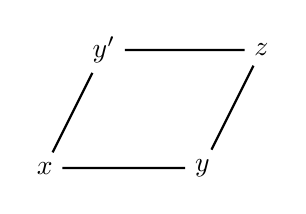
\begin{tikzpicture}
    \node (bl) at (0,0) {$x$};
    \node (br) at (2,0) {$y$};
    \node (tl) at (0.75,1.5) {$y'$};
    \node (tr) at (2.75,1.5) {$z$};
    \draw[thick] (bl) to (tl) to (tr) to (br) to (bl);
  \end{tikzpicture}
\] So
\[\mbox{$xRSz$ iff $x-y$ is in $R$ and $y-z$ is in $S$ for some $y$,}\]
while
\[\mbox{$xSRz$ iff $x-y'$ is in $S$ and $y'-z$ is in $R$ for some $y'$.}\]
but the picture shows these are equivalent!

If we start with a vector space over the reals, complexes or
quaternions, the lattice we get this way is exactly the same as the
lattice we get starting from the corresponding projective space, so
Desargues' theorem in this case is just a corollary of the fact that
Desargues' theorem holds for all linear lattices.

On the other hand, since the lattice associated to the octonionic
projective plane does \emph{not} satisfy Desargues' theorem, it's not a
linear lattice. Maybe someday I'll use these ideas to understand what's
weird about octonionic quantum mechanics.

But another cool thing is that Mark Haiman has cooked up a set of
deduction rules that let you derive precisely all the implications that
hold in all linear lattices. Even better, there's a way to draw pictures
of these deduction rules, which makes them look a bit like tricks for
rewiring electrical circuits! You can learn about this in the above
paper, or Haiman's original paper:

\begin{enumerate}
\def\labelenumi{\arabic{enumi})}
\setcounter{enumi}{3}
\tightlist
\item
  Mark Haiman, ``Proof theory for linear lattices'', \emph{Adv. Math.}
  \textbf{58} (1985), 209--242.
\end{enumerate}

or this followup:

\begin{enumerate}
\def\labelenumi{\arabic{enumi})}
\setcounter{enumi}{4}
\tightlist
\item
  D. Finberg, M. Mainetti and G.-C. Rota, ``The logic of commuting
  equivalence relations'', in \emph{Logic and Algebra}, eds.~A. Ursini
  and P. Agliano, Lecture Notes in Pure and Applied Mathematics,
  vol.~\textbf{180}, Decker, New York 1996.
\end{enumerate}

To finish up, let me add that there are lots of linear lattices. For
example, we can try generalizing the above trick from vector spaces to
groups! Given any group \(G\), each subgroup \(H\) determines an
equivalence relation on \(G\), which by abuse of language I'll call
\(H\), such that \(xHy\) iff \(xy^{-1}\) is in \(H\). If \(G\) is
abelian all these equivalence relations commute, so the lattice of
subgroups of \(G\) becomes a linear lattice. If \(G\) is nonabelian this
trick breaks down unless we use \emph{normal} subgroups.

I should also add that nobody has figured out whether the collection of
linear lattices can be characterized by identities\ldots{} though they
satisfy lots of interesting identities, like the famous ``modular law'':
\[x \operatorname{and} (y \operatorname{or} (x \operatorname{and} z)) = (x \operatorname{and} y) \operatorname{or} (x \operatorname{and} z)\]
This is one reason Haiman's proof theory is interesting.

Now, on to some category theory!

Michael Mueger has written some excellent papers on the relation between
quantum field theory, category theory, and topology:

\begin{enumerate}
\def\labelenumi{\arabic{enumi})}
\setcounter{enumi}{5}
\tightlist
\item
  Michael Mueger, ``Conformal field theory and Doplicher-Roberts
  reconstruction'', available at
  \href{https://arxiv.org/abs/math-ph/0008027}{\texttt{math-ph/0008027}}.
\end{enumerate}

``From subfactors to categories and topology I: Frobenius algebras in
and Morita equivalence of tensor categories'', available at
\href{https://arxiv.org/abs/math.CT/0111204}{\texttt{math.CT/0111204}}.

``From subfactors to categories and topology II: The quantum double of
tensor catgories and subfactors'', available at
\href{https://arxiv.org/abs/math.CT/0111205}{\texttt{math.CT/0111205}}.

I can't possibly do justice to these, but I'd like to discuss a very
pretty idea from his paper on Frobenius algebras. This will give me a
good chance to continue some themes from my earlier issues on
\(n\)-categories and homotopy theory.

In \protect\hyperlink{week83}{``Week 83''} I talked about adjoint
functors, and more generally, adjunctions in any 2-category. If you
don't understand this stuff, you're a goner now, but let me just remind
you of the definitions. Suppose \(a\) and \(b\) are objects in a
2-category. Then we say the morphism \[L\colon a \to b\] is a ``left
adjoint'' of the morphism \[R\colon b \to a\] (and \(R\) is a ``right
adjoint'' of \(L\)) if there are 2-morphisms called the ``unit''
\[i: 1a \Rightarrow LR\] and ``counit'' \[e: RL \Rightarrow 1b\]
satisfying the ``triangle equations'', which say that these vertical
composites are both identity 2-morphisms:
\[L = 1_aL \xRightarrow{i\cdot1_L} LRL \xRightarrow{1_L\cdot e} L1_a = L\]
and
\[R = R1_b \xRightarrow{1_R\cdot i} RLR \xRightarrow{e\cdot1_R} 1_bR = R\]
where \(\cdot\) denotes horizontal composition. The whole setup
\((a,b,L,R,e,i)\) is then called an ``adjunction''.

There are some important variations on this theme. For example, if \(e\)
and \(i\) are invertible, but we drop the triangle equations, we call
the setup an ``equivalence''. It's morally correct to consider two
objects \(a\) and \(b\) in a 2-category ``the same for all practical
purposes'' if they take part in an equivalence. A special case is when
they are \emph{equal} --- since then we can take \(L,R,e,i\) to be
identities. Another special case is when they are \emph{isomorphic} -
since then we can take \(L\) to be an isomorphism, \(R\) its inverse,
and \(e\) and \(i\) to be identities. But in general we only need \(L\)
and \(R\) to be isomorphisms ``up to 2-isomorphism''.

So, the notion of equivalence is better than equality, because it
follows the fundamental principle of \(n\)-category theory: everything
is only true up to something!

If \(e\) and \(i\) are invertible and we \emph{keep} the triangle
equations, we call the setup an ``adjoint equivalence''. In other words,
an adjoint equivalence is an adjunction that is also an equivalence.
This is a bit better than an equivalence. Recently on the category
theory mailing list Paul Levy asked exactly how much better. The first
answer is: not much, because given any equivalence we can cook up an
adjoint equivalence by just fiddling with either the unit or counit in a
standard way, using only the material at hand: \((a,b,R,L,i,e)\). I
leave this as a fun exercise\ldots.

But the second answer, which James Dolan and I worked out this Friday,
goes like this:

First, consider the ``Platonic idea of an equivalence''. By this, I mean
the 2-category \(\mathsf{Equiv}\) which is freely generated by objects
\(a\) and \(b\), morphisms \(L\colon a \to b\) and \(R\colon b \to a\),
and isomorphisms \(i\colon 1_b \Rightarrow RL\) and
\(e\colon LR \Rightarrow 1_a\). Why do I call this the ``Platonic idea
of an equivalence''? Well, any equivalence in any 2-category
\(\mathcal{C}\) is just the same as a 2-functor
\[F\colon \mathsf{Equiv} \to \mathcal{C}\] The functor \(F\) turns the
``abstract'' equivalence in \(\mathsf{Equiv}\) into a ``concrete''
equivalence in \(\mathcal{C}\)! This is reminiscent of Plato's theory of
ideas and how they get manifested in concrete situations. We can think
of \(\mathsf{Equiv}\) as the unadorned idea of an adjunction without any
contamination by accidental extra features.

I should add that James, less of an intellectual snob than I, calls
\(\mathsf{Equiv}\) the ``walking equivalence''. After all, if someone
has really big bushy eyebrows, so that when you see him walking down the
street you first notice his eyebrows and only later realize there's a
person attached, you call him a ``walking pair of eyebrows''. The person
is basically just the life support system for the eyebrows! Similarly,
in \(\mathsf{Equiv}\) we have a 2-category which is just the life
support system for an adjunction: no more and no less.

Anyway, the walking equivalence is a weak 2-groupoid: a 2-category where
every 2-morphism is invertible and every morphism is invertible up to
2-isomorphism. Weak 2-groupoids are secretly the same thing as homotopy
2-types: roughly speaking, topological spaces whose homotopy groups
vanish above dimension 2. And there's a pretty easy way to turn a weak
2-groupoid into a homotopy 2-type. First you turn it into a simplicial
set, called its ``nerve'', and then you take the geometric realization
of that.

Eh? Well, I talked about geometric realization in part E of
\protect\hyperlink{week116}{``Week 116''}, and I talked about the nerve
of a 1-category in part J of \protect\hyperlink{week117}{``Week 117''},
so the only thing I need to do is say a bit about the nerve of a
2-category. This is a simplicial set where the 0-simplices correspond to
objects: \[x\] the 1-simplices correspond to morphisms:
\[x\xrightarrow{F}Y\] the 2-simplices correspond to 2-morphisms: \[
  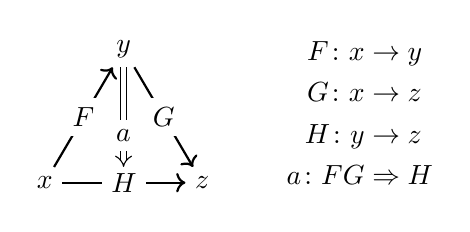
\begin{tikzpicture}
    \node (x) at (0,0) {$x$};
    \node (y) at (1,1.7) {$y$};
    \node (z) at (2,0) {$z$};
    \draw[thick,->] (x) to node[fill=white]{$F$} (y);
    \draw[thick,->] (x) to node[fill=white]{$H$} (z);
    \draw[thick,->] (y) to node[fill=white]{$G$} (z);
    \draw[double,double equal sign distance,-implies] (y) to (1,0.2);
    \node[fill=white] at (1,0.6) {$a$};
    \node at (4,0.85) {$
      \begin{aligned}
        F\colon x&\to y
      \\G\colon x&\to z
      \\H\colon y&\to z
      \\a\colon FG&\Rightarrow H
      \end{aligned}
    $};
  \end{tikzpicture}
\] and the higher-dimensional simplices correspond to equations,
``equations between equations'', and so on.

Anyway, if you use this trick to turn the walking equivalence into a
space, what space do you get?

The 2-sphere!

It's pretty easy to see\ldots{} I'd draw it for you on paper if I could,
but you'll have to do it yourself. It helps if you have a globe:

\begin{itemize}
\tightlist
\item
  \(a\) is the North Pole,
\item
  \(b\) is the South Pole,
\item
  \(L\colon a \to b\) is the Greenwich Meridian running from north to
  south,
\item
  \(R\colon b \to a\) is the International Date Line running from south
  to north,
\item
  \(i\colon 1_a \Rightarrow LR\) is the Eastern Hemisphere, and
\item
  \(e\colon RL \Rightarrow 1_b\) is the Western Hemisphere!
\end{itemize}

(More precisely, we just get the 2-sphere up to homotopy equivalence:
there is a whole bunch of higher-dimensional flab which I'm ignoring
here. But that's okay, since we're doing homotopy theory.)

We can also play this game for the ``walking adjoint equivalence'',
\(\mathsf{AdEquiv}\). This is just like the walking equivalence, except
we put in extra relations: the triangle equations. How does this affect
the space we get?

It's very beautiful: the extra equations fill in the 2-sphere to give us
a 3-ball! (At least up to homotopy equivalence.)

Now, the 3-ball is contractible, so as a homotopy type it's really the
same as a point. And a point is exactly the space we'd get from playing
the same game starting with the ``walking object'': the 2-category with
one object, its identity morphism, and the identity 2-morphism of that.

To the eyes of a homotopy theorist, a point and 3-ball are the same, but
the 2-sphere is not. Similarly, to the eyes of an \(n\)-category
theorist, the walking object and the walking adjoint equivalence are
``the same'', but the walking equivalence is not!

We could make this very precise with a suitable notion of ``sameness''
for 2-categories. But instead, let's jump straight to the punchline:
having an adjoint equivalence in a 2-category is ``the same'' as having
an object\ldots. but having an equivalence is not!

There's even more fun to be had here. Since every adjoint equivalence is
an equivalence, there's a 2-functor
\[I\colon \mathsf{Equiv} \to \mathsf{AdEquiv}\] But I also said every
equivalence can be massaged to obtain an adjoint equivalence! In fact, I
said it could be done in two equally good ways. Either of these gives a
2-functor \[P\colon \mathsf{AdEquiv} \to \mathsf{Equiv}\] Now, we can
ask what these become when we turn them into maps between spaces\ldots.

It turns out that \(I\) is just the inclusion of the 2-sphere into the
3-ball, while \(P\) is the map that squashes the 3-ball down to either
the eastern or western hemisphere of the sphere!

By the way, it is irresistible to predict generalizations to higher
dimensions. For any \(n\), we will have weak \(n\)-groupoids called
\(\mathsf{Equiv}\), the ``walking \(n\)-equivalence'', and
\(\mathsf{AdEquiv}\), the ``walking adjoint n-equivalence''. The
geometric realization of the nerve of \(\mathsf{Equiv}\) will be
homotopy equivalent to the \(n\)-sphere, while that of
\(\mathsf{AdEquiv}\) will be homotopy equivalent to the \((n+1)\)-ball.

(Note that for \(n = 1\), \(\mathsf{Equiv}\) will be the category with
objects \(a\) and \(b\) and isomorphisms \(L\colon a \to b\),
\(R\colon b \to a\). In \(\mathsf{AdEquiv}\), there will be extra
relations saying that \(R\) is the inverse of \(L\). In this sense, it
is really an adjoint equivalence rather than an equivalence which is the
proper generalization of an isomorphism!)

Okay. Believe it or not, I still haven't gotten to the stuff Michael
Mueger was talking about! I got distracted. I talked about the walking
equivalence and the walking adjoint equivalence, but next week, I'll
talk about the walking adjunction\ldots{} and finally the walking
``biadjunction'', which is where Mueger comes in.

\begin{center}\rule{0.5\linewidth}{0.5pt}\end{center}

Postscript --- Keith Harbaugh writes:

\begin{quote}
Since you're back on Desargues again, just thought I'd mention (in case
you haven't already noticed this) that if you look up Desargues in
``Categories, Allegories'' by Freyd and Scedrov, you'll find that they
(probably really Freyd) have a neat proof of Desargues in the context of
their ``allegories'' (2-categories with structure modeled on the
bicategory of relations).
\end{quote}

Linus Kramer writes:

\begin{quote}
I'd like to comment on the interesting paper by Thomas Püttmann and A.
Rigas, Isometric actions on the projective planes and embedded
generators of homotopy groups, available at

\texttt{http://www.ruhr-uni-bochum.de/mathematik8/puttmann/index.html}

which is mentioned in Baez' article.

As Baez writes, the authors construct an embedding of the 11-sphere into
the Cayley plane \(\mathbb{OP}^2\). This embedding is closely related to
a polarity (a polarity of a projective plane is an involution which maps
points to lines and vice versa, and which preserves incidence).

The simplest example is the elliptic polarity over the reals. Take the
standard inner product on R\^{}3 and consider the map which sends a
subspace to its perp. Now the points of the real projective plane are
the 1-dimensional subspaces, and the lines are the 2-dimensional
subspaces. It is fairly easy to see that this map `take the perp' is a
polarity.

Now there is also a different polarity: take a Minkowski-like metric on
\(\mathbb{R}^3\), (\(++-\)). In exactly the same way as above, one
obtains a polarity, the hyperbolic polarity of the real projective
plane. This polarity has absolute elements, i.e.~elements which are
incident with their image under the polarity: this happens with all
1-dim. subspaces which are `light-like', i.e.~on which the metric
vanishes. The set of all absolute points in \(\mathbb{RP}^2\) is a
1-sphere.

One can prove that up to automorphisms, these two are the only
polarities for the real projective plane \(\mathbb{RP}^2\). Notice the
associated motion groups \(\mathrm{SO}_3(\mathbb{R})\) and
\(\mathrm{SO}_{2,1}(\mathbb{R})\) (the motion group consists of all
collineations which commute with the polarity).

Similar polarities can be defined for the complex, the quaternionic and
the octonionic projective planes. One obtains elliptic (no absolute
points) and hyperbolic (many absolute points) polarities. In the second
case, the set of absolute points are spheres of dimensions 3,7,15,
respectively.

But for these latter projective planes, there are more polarities! There
is one more polarity (called `planar polarity' by some authors) which
has a different kind of absolute points. For these polarities, one
obtains spheres of dimension 2,5,11, respectively for the absolute
points.

These semi-classical embeddings were (re)discovered by the authors. The
corresponding motion groups are by the way simple; they are
\(SO_{3,1}(\mathbb{R})\), \(SU_{3,1}(\mathbb{C})\) and
\(SU_{3,1}(\mathbb{H})=\mathrm{Sp}_{3,1}\). If one looks only for
isometric motions (as the authors do) (i.e.~motions which centralize at
the same time the elliptic polarity) one obtains the compact groups
mentioned in the article.

Of course, the main point of the authors is that they obtain generators
of the 11th homotopy group, and this is certainly a new and beautiful
result. I just wanted to mention some related `classical' results from
projective geometry.

A good source here is, as always, Salzmann et al., Compact Projective
Planes, de Gruyter 1995, p.~127.

Regards, Linus Kramer
\end{quote}

\begin{center}\rule{0.5\linewidth}{0.5pt}\end{center}
\hypertarget{week174}{%
\section{DATE}\label{week174}}

Groups are how mathematicians and physicists talk about symmetry, and
Lie groups are how they talk about \emph{continuously varying}
symmetries, like rotations, translations and the like. Sophus Lie helped
start the subject of Lie groups in the late 1800s, and it's been in
constant growth ever since. I spend lots of time studying it, and I
probably will all my life --- there's a lot to learn! To really
understand it, it helps to know the history. And for that, this is the
book to read:

\begin{enumerate}
\def\labelenumi{\arabic{enumi})}
\tightlist
\item
  Thomas Hawkins, \emph{The Emergence of the Theory of Lie Groups: an
  Essay in the History of Mathematics, 1869--1926}, Springer, New York,
  2000.
\end{enumerate}

You have to know your Lie groups pretty well to enjoy this book, but if
you do, you'll find it's full of interesting facts. For example: folks
often complain about Wilhelm Killing's original classification of simple
Lie algebras --- it wasn't rigorous, he made some mistakes, and so on.
Elie Cartan came along later and cleaned it up, and many people applaud
Cartan's work and sneer at poor old Killing, even though he was the one
who came up with the original ideas. But in this book, it becomes clear
that Killing was pretty much \emph{pushed} into publishing his ideas in
a half-baked state by mathematicians who were dying to know his results!
Now I feel even more sorry for him.

There's also a lot of interesting stuff about Hermann Weyl's approach to
representation theory via tensors and Young diagrams, and why he liked
it better than Cartan's approach via roots and weights. Basically, Weyl
liked his approach because it stuck closer to Felix Klein's original
``Erlanger program'' --- a program for understanding geometry via
symmetry groups. But it's interesting to see how Weyl studied and
respected Cartan's approach, and tried to bridge the gap between the
two.

Okay\ldots{} so much for gossip! Now I'm going to dive in and pick up
right where I left off in my discussion of the ideas behind this paper:

\begin{enumerate}
\def\labelenumi{\arabic{enumi})}
\setcounter{enumi}{1}
\tightlist
\item
  Michael Mueger, ``From subfactors to categories and topology I:
  Frobenius algebras in and Morita equivalence of tensor categories'',
  available at
  \href{https://arxiv.org/abs/math.CT/0111204}{\texttt{math.CT/0111204}}.
\end{enumerate}

My ultimate goal is to take you to an elegant understanding of Frobenius
algebras by means of a 2-category called the ``walking ambidextrous
adjunction'', but first I'll play around a bit with a simpler but more
famous 2-category called the ``walking adjunction''. This may sound
scary, but if you can stick with it, you'll see that I'm really just
using these 2-categories to describe fun games that you can play with
certain 2-dimensional pictures. Even if you don't read the words, please
stare at the pictures --- I spend my Thanksgiving weekend drawing them,
and I don't want that work to go to waste!

Category theorists love to talk about adjoint functors, but 2-category
theorists know that these are just a special example of an
``adjunction''. An adjunction is something that makes sense in any
2-category; if we take the 2-category to be \(\mathsf{Cat}\) we get
adjoint functors. There are lots of other nice examples that make this
generalization worthwhile. For example, in
\protect\hyperlink{week83}{``Week 83''} I explained how a pair of dual
vector spaces is also an example of an adjunction.

To study adjunctions, it suffices to study the ``walking adjunction''.
This is a little 2-category containing exactly the stuff any adjunction
in any 2-category must have: not a jot more, not a tiddle less! It was
first studied by Schanuel and Street:

\begin{enumerate}
\def\labelenumi{\arabic{enumi})}
\setcounter{enumi}{2}
\tightlist
\item
  Stephen Schanuel and Ross Street, ``The free adjunction'', \emph{Cah.
  Top. Geom. Diff.} \textbf{27} (1986), 81--83.
\end{enumerate}

In a bit more detail, the walking adjunction is the 2-category freely
generated by two objects: \[\mbox{$a$ and $b$,}\] two morphisms:
\[\mbox{$L\colon a \to b$ and $R\colon b \to a$,}\] and two 2-morphisms,
called the ``unit'' and ``counit'':
\[\mbox{$i\colon 1_a \Rightarrow LR$ and $e\colon RL \Rightarrow 1_b$}\]
satisfying two relations, called the ``triangle equations''.

I wrote down these equations already last week, but let me do it again
using ``string diagrams'', as explained in
\protect\hyperlink{week79}{``Week 79''} and
\protect\hyperlink{week92}{``Week 92''}. In a 2-categorical string
diagram, objects are denoted by 2d regions in the plane, morphisms are
denoted by 1d edges, and 2-morphisms are denoted by 0d points. If the
dimensions look sort of upside-down, you're right --- that's exactly the
point!

Instead of explaining the whole theory, I'll just plunge in with the
example at hand. The unit \(i\) looks like this: \[
  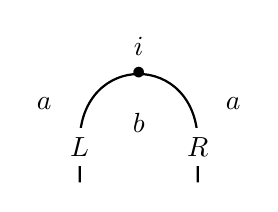
\begin{tikzpicture}[yscale=-1]
    \begin{knot}
      \strand[thick] (0,0)
      to (0,-0.5)
      to [out=down,in=down,looseness=2] (1.5,-0.5)
      to (1.5,0);
    \end{knot}
    \node[fill=white] at (0,-0.45) {$L$};
    \node[fill=white] at (1.5,-0.45) {$R$};
    \node[label={[label distance=-1mm]above:{$i$}}] at (0.75,-1.39) {$\bullet$};
    \node at (0.75,-0.75) {$b$};
    \node at (-0.45,-1) {$a$};
    \node at (1.95,-1) {$a$};
  \end{tikzpicture}
\] while the counit \(e\) looks like this: \[
  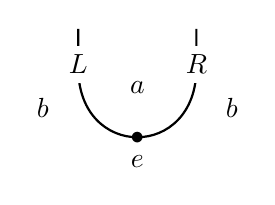
\begin{tikzpicture}
    \begin{knot}
      \strand[thick] (0,0)
      to (0,-0.5)
      to [out=down,in=down,looseness=2] (1.5,-0.5)
      to (1.5,0);
    \end{knot}
    \node[fill=white] at (0,-0.45) {$L$};
    \node[fill=white] at (1.5,-0.45) {$R$};
    \node[label={[label distance=-1mm]below:{$e$}}] at (0.75,-1.39) {$\bullet$};
    \node at (0.75,-0.75) {$a$};
    \node at (-0.45,-1) {$b$};
    \node at (1.95,-1) {$b$};
  \end{tikzpicture}
\] Note that as you cross a line labelled ``\(L\)'' from left to right,
you go from region \(a\) to region \(b\), which is our way of saying
that \(L\colon a\to b\). Similarly, as you cross a line labelled
``\(R\)'' from left to right, you go from region \(b\) to region \(a\),
since \(R\colon b\to a\).

In terms of string diagrams, the triangle equations just say that we can
straighten out a zig-zag: \[
  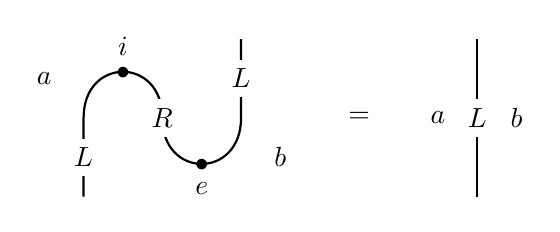
\begin{tikzpicture}
    \begin{scope}
      \begin{knot}
        \strand[thick] (0,0)
        to (0,1)
        to [out=up,in=up,looseness=2] (1,1)
        to [out=down,in=down,looseness=2] (2,1)
        to (2,2);
      \end{knot}
      \node at (-0.5,1.5) {$a$};
      \node[fill=white] at (0,0.5) {$L$};
      \node[label={[label distance=-1mm]above:{$i$}}] at (0.5,1.57) {$\bullet$};
      \node[fill=white] at (1,1) {$R$};
      \node[label={[label distance=-1mm]below:{$e$}}] at (1.5,0.4) {$\bullet$};
      \node[fill=white] at (2,1.5) {$L$};
      \node at (2.5,0.5) {$b$};
    \end{scope}
    \node at (3.5,1) {$=$};
    \begin{scope}[shift={(5,2)}]
      \node at (-0.5,-1) {$a$};
      \draw[thick] (0,0) to node[fill=white]{$L$} (0,-2);
      \node at (0.5,-1) {$b$};
    \end{scope}
  \end{tikzpicture}
\] or a zag-zig: \[
  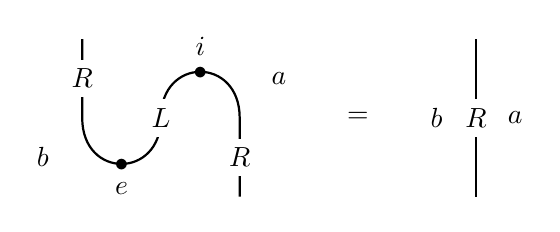
\begin{tikzpicture}
    \begin{scope}[xscale=-1,shift={(-2,0)}]
      \begin{knot}
        \strand[thick] (0,0)
        to (0,1)
        to [out=up,in=up,looseness=2] (1,1)
        to [out=down,in=down,looseness=2] (2,1)
        to (2,2);
      \end{knot}
      \node at (-0.5,1.5) {$a$};
      \node[fill=white] at (0,0.5) {$R$};
      \node[label={[label distance=-1mm]above:{$i$}}] at (0.5,1.57) {$\bullet$};
      \node[fill=white] at (1,1) {$L$};
      \node[label={[label distance=-1mm]below:{$e$}}] at (1.5,0.4) {$\bullet$};
      \node[fill=white] at (2,1.5) {$R$};
      \node at (2.5,0.5) {$b$};
    \end{scope}
    \node at (3.5,1) {$=$};
    \begin{scope}[shift={(5,2)}]
      \node at (-0.5,-1) {$b$};
      \draw[thick] (0,0) to node[fill=white]{$R$} (0,-2);
      \node at (0.5,-1) {$a$};
    \end{scope}
  \end{tikzpicture}
\] We can build any 2-morphism in the walking adjunction by vertically
and horizontally composing units and counits, which corresponds to
sticking together string diagrams in a vertical or horizontal way. Thus,
a typical 2-morphism looks like this:

\begin{verbatim}
      \     \   a   /   \   a   /      /               |
       \     R     L     R     L      /       i        |
        \     \   /       \   /      /       / \       L
         \     \ /         \ /      /   a   /   R      |    b
          \     e           e      /       /     \     |
    a      L                      R        \      \   / 
            \         b          /     i    \      \ / 
             \                  /     / \    L      e
              \                /     L   R    \       
               \              /     /  b  \    \  
\end{verbatim}

By the triangle equations, we could straighten out the zig-zag without
changing the 2-morphism.

As you may know, the word ``anaranjado'' means ``orange'' in Spanish ---
there was no word in English for ``orange'' before people in England
started importing oranges from Spain. And this is a nice mnemonic,
because if we take the above picture and paint the regions labelled
``\(a\)'' orange, and paint the regions labelled ``\(b\)'' black, the
above picture has a roughly tiger-striped appearance. In fact, these
tiger stripes tell you everything you need to know about the 2-morphism!
For example, starting from just this:

\begin{verbatim}
      \     \   a   /   \   a   /      /               |
       \     \     /     \     /      /       _        |
        \     \   /       \   /      /       / \       |
         \     \_/         \_/      /   a   /   \      |    b
          \                        /       /     \     |
    a      \                      /        \      \   / 
            \         b          /     _    \      \_/ 
             \                  /     / \    \      
              \                /     /   \    \       
               \              /     /  b  \    \  
\end{verbatim}

you can figure out where everything else should go.

By the way, note that orange stripes can disappear as we go down the
page, and they can split, but they can't appear or merge. Black stripes
can appear or merge, but they can't disappear or split. As a result,
there can never be any orange or black \emph{spots}. We'll change these
rules later, when we talk about the walking ``ambidextrous adjunction''.

Okay, so we've got this 2-category, the walking adjunction: let's call
it \(\mathsf{Ad}\) for short. It's pretty simple. How can we understand
it better?

Well, for any two objects \(a\) and \(b\) in a 2-category we get a
``hom-category'' \(\operatorname{Hom}(a,b)\), whose objects are the
morphisms from \(a\) to \(b\), and whose morphisms are the 2-morphisms
between those. If we work out these hom-categories in \(\mathsf{Ad}\),
we get some cool stuff.

First let's look at the hom-category \(\operatorname{Hom}(a,a)\). In
this category, the objects are \[1_a, LR, LRLR, LRLRLR, \ldots\] and all
the morphisms are built by sticking these two basic generators together
vertically or horizontally:

\begin{verbatim}
                     \  \    a    /  /  
                      \  \       /  /
                       L  R     L  R
                        \  \   /  /
                  a      \  \ /  /      a
                          \  e  /
                           \   /
                           | b |
                           |   |
                           L   R
                           |   |
                           |   |   
\end{verbatim}

and

\begin{verbatim}
                              i
                             / \
                     a      |   |    a
                            | b |     
                            |   |
                            L   R   
                            |   |
                            |   |
\end{verbatim}

In tiger language, we're talking about pictures of black stripes on an
orange background. The two basic generators are the merging of two black
stripes and the appearance of a black stripe.

If you read \protect\hyperlink{week89}{``Week 89''}, you'll know another
way to describe this! Our ability to stick together pictures vertically
and horizontally makes \(\operatorname{Hom}(a,a)\) into a ``monoidal
category''. \(LR\) is a ``monoid object'', with merging of two black
stripes being ``multiplication'', and the appearance of a black stripe
being the ``multiplicative identity''. Being a ``monoid object'' simply
means that these operations satisfy the left unit law:

\begin{verbatim}
                                 / /                 | |
                                / /                  | |
                               / /                   | |
                    /\        / /                    | |
                    \ \      / /                     | |
                     \ \    / /                      | |
                      \ \  / /                  a    | |
                       \ \/ /                        |b|
                        |  /          =              | |
             a          | |                          | |      a
                        | |                          | |
                        |b|                          | |
                        | |     a                    | |
                        | |                          | |
                        | |                          | |
                        | |                          | |
\end{verbatim}

and its mirror image, called the right unit law, together with the
associative law:

\begin{verbatim}
            \ \  a / /    / /      \ \    \ \  a / /
             \ \  / /  a / /        \ \  a \ \  / /
              \ \/ /    / /          \ \    \ \/ /
               \  /    / /            \ \    \  /
                \ \   / /              \ \   / /
                 \ \_/ /                \ \_/ /
                  \   /                  \   /
                   | |                    | |
              a    | |   a            a   | |   a
                   | |          =         | |
                   |b|                    |b|
                   | |                    | |
                   | |                    | |
                   | |                    | |
                   | |                    | |
\end{verbatim}

There aren't any other laws, so \(\operatorname{Hom}(a,a)\) is the
``free monoidal category on a monoid object'', or if you prefer, the
``walking monoid''!

I touched upon the immense consequences of this fact for algebraic
topology in \protect\hyperlink{week117}{``Week 117''} and
\protect\hyperlink{week118}{``Week 118''}. They mainly rely on another
way of thinking about \(\operatorname{Hom}(a,a)\): it's the category of
order-preserving maps between finite ordinals!

For example, these black tiger stripes on an orange background:

\begin{verbatim}
         0          1           2                     3
    --------------------------------------------------------
   |  \     \   a |   |  a  /      /               |    |   |
   |   \     \    |   |    /      /       _        |    |   |
   |    \     \   |   |   /      /       / \       |    |   |
   |     \     \_/     \_/      /   a   /   \      |    |   |
   |      \                    /        \    \     |    |   |
   | a     \                  /          \    \   /    /    |
   |        \       b        /     _      \    \_/    /     |
   |         \              /     / \      \         /      |
   |          \            /     / b \      \   b   /   a   |
   |           \          /     /     \      \     |        |
    --------------------------------------------------------
                     0             1            2
\end{verbatim}

correspond to the order-preserving map
\[f\colon \{0,1,2,3\} \to \{0,1,2\}\] with
\[f(0) = 0,\quad f(1) = 0,\quad f(2) = 0,\quad f(3) = 2.\] Just read the
stripes down!

A more geometrical way to say the same thing is to call
\(\operatorname{Hom}(a,a)\) the category of ``simplices'', usually
denoted \(\Delta\). Here the object
\[\underbrace{LRLR\ldots LR}_{\mbox{$n+1$ of them}}\] corresponds to the
\(n\)-simplex, and these morphisms: \[
  \begin{tikzcd}[column sep=huge]
    1_a
      \rar["i" description]
    & LR
      \rar[shift left=5,"i\cdot LR" description]
      \rar["LR\cdot i" description]
    & LRLR
      \rar[shift left=10,"i\cdot LRLR" description]
      \rar[shift left=5,"LR\cdot i\cdot LR" description]
      \rar["LRLR\cdot i" description]
      \lar[shift left=5,"L\cdot e\cdot R" description]
    & LRLRLR
      \lar[shift left=5,"L\cdot e\cdot RLR" description]
      \lar[shift left=10,"LRL\cdot e\cdot R" description]
      \rar
    &\ldots
  \end{tikzcd}
\]

\begin{verbatim}
                                 -i.LRLR-->
                 --i.LR->        -LR.i.LR->
1a  --i-->  LR  --LR.i->  LRLR  -LRLR.i-->  LRLRLR ...
                 <-L.e.R-        <-L.e.RLR-
                                 <-LRL.e.R-
\end{verbatim}

are the basic ``face'' and ``degeneracy'' maps between simplices, which
you'll find in any book on algebraic topology. The \(n\)-simplex is a
face of the \((n+1)\)-simplex in n+1 ways, and there are n basic
degenerate ways to map the \((n+1)\)-simplex down to the \(n\)-simplex.
These aren't \emph{all} the morphisms; just enough to generate all the
rest by composition --- i.e., sticking together pictures vertically, but
\emph{not} horizontally.

Perhaps I should explain the notation here a bit more. Readers of
\protect\hyperlink{week80}{``Week 80''} will know that I use a dot to
denote horizontal composition of 2-morphisms. For example, when we have
a couple of 2-morphisms like this:

\begin{verbatim}
                      f           f'
                  ---->----   ---->----  
                 /   ||    \ /   ||    \              S: f \Rightarrow g
                x    || S   y    || T   z             T: f' \Rightarrow g'
                 \   \/    / \   \/    /
                  ---->----   ---->----
                      g           g'
\end{verbatim}

we get a 2-morphism like this:

\begin{verbatim}
                         ff'
                  -------->-------
                 /       ||       \
                x        || S.T    z                S.T: ff' \Rightarrow gg'
                 \       \/       /
                  -------->-------
                         gg'
\end{verbatim}

But sometimes we can also horizontally compose a morphism and a
2-morphism! We can do it whenever our morphism \(f\) looks like a little
``whisker'' \(f\) sticking out of the 2-morphism \(T\):

\begin{verbatim}
                                  f'
                              ---->----  
                      f      /   ||    \              
                x----->-----y    || T   z             T: f' \Rightarrow g'
                             \   \/    /
                              ---->----
                                  g'
\end{verbatim}

and what we get is a 2-morphism \(f\cdot S\) like this:

\begin{verbatim}
                         ff'
                  -------->-------
                 /       ||       \
                x        || f.T    z                f.T: ff' \Rightarrow fg'
                 \       \/       /
                  -------->-------
                         fg'
\end{verbatim}

This process, called ``whiskering'', is not really a new operation.
\(f\cdot S\) is really just the horizontal composite of these
2-morphisms:

\begin{verbatim}
                      f           f'
                  ---->----   ---->----  
                 /   ||    \ /   ||    \              
                x    ||1_f  y    || S   z             
                 \   \/    / \   \/    /
                  ---->----   ---->----
                      f           g'
\end{verbatim}

Similarly we can define \(T\cdot f\) in this sort of situation:

\begin{verbatim}
                      f'           
                  ---->----   
                 /   ||    \      f                   T: f' \Rightarrow g'
                x    || T   y----->-----z             T.f: f'f \Rightarrow g'f
                 \   \/    /
                  ---->---- 
                      g'     
\end{verbatim}

Anyway, once you're an expert on this 2-categorical yoga, you can easily
see that these morphisms in \(\operatorname{Hom}(a,a)\), which are
really 2-morphisms in \(\mathsf{Ad}\):

\begin{verbatim}
                                 -i.LRLR-->
                 --i.LR->        -LR.i.LR->
1a  --i-->  LR  --LR.i->  LRLR  -LRLR.i-->  LRLRLR ...
                 <-L.e.R-        <-L.e.RLR-
                                 <-LRL.e.R-
\end{verbatim}

are obtained by taking our basic tiger stripe operations --- the
``merging of two black stripes'', or \(L\cdot e\cdot R\), and the
``appearance of a black stripe'', or \(i\) --- and drawing some extra
black stripes on both sides. That's what those \(LR\)'s are for. After
all, no tiger is complete without whiskers!

Okay. Now, having understood \(\operatorname{Hom}(a,a)\) in all these
ways, let's turn to \(\operatorname{Hom}(b,b)\). Luckily, this is very
similar! Here the objects are
\[1_b,\quad RL,\quad RLRL,\quad RLRLRL,\quad \ldots\] and morphisms are
pictures of \emph{orange} stripes on a \emph{black} background:

\begin{verbatim}
           \   a   /   \   a   /      /               |
            \     /     \     /      /       _        |
             \   /       \   /      /       / \       |
              \_/         \_/      /   a   /   \      |    b
                                  /       /     \     |
                                 /        \      \   / 
       b                        /     _    \      \_/ 
                               /     / \    \      
                              /     /   \    \       
                             /     /  b  \    \  
\end{verbatim}

These orange stripes can only split:

\begin{verbatim}
                           |   |
                           |   |   
                           R   L
                           |   |
                           | a |
                           /   \                           
                          /  i  \
                  b      /  / \  \      b
                        /  /   \  \
                       R  L     R  L
                      /  /       \  \
                     /  /    b    \  \ 
\end{verbatim}

or disappear:

\begin{verbatim}
                            |   |    
                     b      | a |     b 
                            |   |
                            R   L   
                            |   |
                            |   |
                             \ /
                              e
\end{verbatim}

as we march down the page. This means is that
\(\operatorname{Hom}(b,b)\) is \(\Delta^{\mathrm{op}}\): the
\emph{opposite} of the category of simplices, the \emph{opposite} of the
category of finite ordinals, or the walking \emph{comonoid} --- which is
just like a monoid, only upside down!

Here is another picture of \(\operatorname{Hom}(b,b)\):

\begin{verbatim}
                                  --R.i.LRL->
                 --R.i.L->        --RLR.i.L->
1b  <--e--  RL  <--e.RL--  RLRL  <--e.RLRL--  RLRLRL ...
                 <--RL.e--        <--RL.e.RL-
                                  <--RLRL.e--
\end{verbatim}

If you're a devoted reader of This Week's Finds, you'll know I secretly
drew this category already in section N of
\protect\hyperlink{week118}{``Week 118''}. There I was talking about
specific adjoint functors instead of the walking adjunction, so as not
to prematurely blow your mind. I was also writing horizontal composites
backwards, for certain old-fashioned reasons. But the idea is exactly
the same! The morphisms above give the usual ``face and degeneracy
maps'' we always have in a simplicial set, since a simplicial set is a
functor \[F\colon \Delta^{\mathrm{op}} \to \mathsf{Set}.\] By the way,
you may have noticed that to get from \(\operatorname{Hom}(a,a)\) to
\(\operatorname{Hom}(b,b)\), we had to switch the colors orange and
black AND read the pictures upside-down. The reason is that if we turn
around all the 1-morphisms AND 2-morphisms in the walking adjunction, we
get the walking adjunction again. Ponder that!

We can summarize what we've learned so far using the ``Platonic idea''
jargon I introduced last week:

\begin{quote}
The Platonic idea of a monoid and the Platonic idea of a comonoid are
the hom-categories \(\operatorname{Hom}(a,a)\) and
\(\operatorname{Hom}(b,b)\) sitting inside the Platonic idea of an
adjunction!
\end{quote}

(By the way, to round this off we should really describe
\(\operatorname{Hom}(a,b)\) and \(\operatorname{Hom}(b,a)\), too. I
think \(\operatorname{Hom}(a,b)\) is the Platonic idea of ``an object
with a left action of a monoid and a right coaction of a comonoid, in a
compatible way''. If so, \(\operatorname{Hom}(b,a)\) would be the
Platonic idea of ``an object with a right action of a monoid and a left
coaction of a comonoid, in a compatible way''. By ``compatible'' I'm
saying that we can act on one side and coact on the other side in either
order, and get the same thing. Filling in the details requires concepts
I'm not eager to discuss right now, so I leave this as an exercise for
the highly energetic reader. The less energetic reader can just study
the tiger-stripe descriptions of these categories.)

Finally, here's Mueger's new twist on all these ideas! Better than an
adjunction is an ``ambidextrous'' adjunction. This has some extra
structure, which turns out to explain all sorts of fancy-sounding stuff
people look at in the study of subfactors and TQFTs and the like\ldots.

But what's an ``ambidextrous adjunction''?

A ambidextrous adjunction is where you have a morphism
\[L\colon a \to b\] in a 2-category that is both left and right adjoint
to \[R\colon b \to a.\] More precisely, it is a setup
\[(a,b,L,R,i,e,j,f)\] where \[(a,b,L,R,i,e)\] and \[(b,a,R,L,j,f)\] are
both adjunctions.

In terms of string diagrams, our generating 2-morphisms look like this:

\begin{verbatim}
                  i                             j
                 / \                           / \
                L   R                         R   L
               /     \                       /     \
           a  /   b   \  a               b  /   a   \  b




           b  \   a   /  b               a  \   b   /  a
               R     L                       L     R
                \   /                         \   /
                 \ /                           \ /
                  e                             f
\end{verbatim}

and the triangle equations say all possible zig-zags can be straightened
out.

Now let's study the ``walking ambidextrous adjunction'',
\(\mathsf{AmbAd}\). As before, 2-morphisms in \(\mathsf{AmbAd}\) can be
described using pictures with orange and black stripes --- but now
\emph{both} kinds of stripes can appear, disappear, merge or split as we
march down the page:

\begin{verbatim}
  -------------------------------------------------------
 |   \     \   a |   |  a  /      /             |       |
 |    \     \    |   |    /      /              |       |
 |     \     \__/     \__/      /      a        |       |
 |      \        _____         /     _____      |       |
 |       \      /  a  \       /     /     \     |       |
 |  a    /     /  ___  \     /     /       \   /        |
 |      /     /  /   \  \   /     /    __   \_/         |
 |     /     /   \ b /  /  /     /    /  \              |
 |    /  b   \    \_/  /  /     /    / a  \  b          |
 |   /        \       /  /     /    /      \            |
  -------------------------------------------------------
\end{verbatim}

This allows for quite arbitrary ways of cutting up a rectangle into
regions of orange and black, with piecewise linear boundaries, subject
to the condition that each vertical border has the same color all along
it. The triangle equations and the rules for 2-categories say that we
can warp such a picture around without changing the 2-morphism that it
defines\ldots{} I don't want to be too precise here, since it would be
boring. Hopefully you get the idea: AmbAd has a purely topological
description!

Now for the punchline: in \(\mathsf{AmbAd}\), what is the category
\(\operatorname{Hom}(a,a)\) like? As in \(\mathsf{Ad}\), the objects are
\[1_a,\quad LR,\quad LRLR,\quad LRLRLR,\quad \ldots\] but now the object
LR is equipped not only with multiplication:

\begin{verbatim}
                     \  \    a    /  /  
                      \  \       /  /
                       L  R     L  R
                        \  \   /  /
                  a      \  \ /  /      a      
                          \  e  /                     multiplication:
                           \   /                     L.e.R: LRLR \Rightarrow LR 
                           | b |
                           |   |
                           L   R
                           |   |
                           |   |   
\end{verbatim}

and multiplicative identity:

\begin{verbatim}
                             i
                            / \
                    a      |   |    a                 multiplicative
                           | b |                         identity:
                           |   |                        i: 1a \Rightarrow LR
                           L   R   
                           |   |
                           |   |
\end{verbatim}

but also a ``comultiplication'':

\begin{verbatim}
                           |   |
                           |   |   
                           L   R
                           |   |
                           | b |
                           /   \                           
                          /  j  \                    comultiplication:
                  a      /  / \  \      a            L.j.R: LR \Rightarrow LRLR
                        /  /   \  \
                       L  R     L  R
                      /  /       \  \
                     /  /    b    \  \ 
\end{verbatim}

and ``comultiplicative coidentity'':

\begin{verbatim}
                            |   |    
                     a      | b |     a 
                            |   |                    comultiplicative
                            L   R                       coidentity:
                            |   |                      f: LR \Rightarrow 1a
                            |   |
                             \ /
                              f
\end{verbatim}

which make it into a monoid object \emph{and} a comonoid object. Even
better, there are some extra relations between the multiplication and
comultiplication, which make LR into a so-called ``Frobenius object''!

In short, \(\operatorname{Hom}(a,a)\) is the walking Frobenius object!
So is \(\operatorname{Hom}(b,b)\), since there is no real asymmetry
between the objects \(a\) and \(b\) in an ambidextrous adjunction, as
there was with an adjunction. I haven't thought much about
\(\operatorname{Hom}(a,b)\) and \(\operatorname{Hom}(b,a)\) yet, but one
obvious thing is that they're isomorphic.

Next time I'll talk about examples of Frobenius objects and why they are
so important in subfactors, TQFTs and the like. This is what Mueger is
really interested in. Right now, I want to wrap up by saying exactly
what it means to say \(LR\) is a ``Frobenius object''. What are the
extra relations between multiplication and comultiplication?

There are various ways of describing these relations. Mueger uses a pair
of equations that are popular in the TQFT literature:

\begin{verbatim}
               \ \     / /                | |        | |
                \ \   / /                 | |        | |
                 \ \_/ /                  | |        | |
                  \   /                   |  \   a   | |
                   | |                    |   \      | |
              a    | |   a           a    | |\ \     | |   a
                   | |                    | | \ \    | |
                   |b|                    | |  \ \   | |
                   | |          =         | |   \ \  | |
                   | |                    | |    \ \ | |
                   | |                    | |  a  \ | |
                   | |                    | |      \   |
                  / _ \                   | |       \ b|
                 / / \ \                  | |        | |
                / /   \ \                 | |        | | 
               / /     \ \                | |        | |
\end{verbatim}

and its mirror image. People sometimes call these the ``\(I = N\)''
equations, for the obvious reason. So: one definition of a ``Frobenius
object'' in a monoidal category is that it's a monoid object / comonoid
object satisfying the \(I = N\) equations.

Where can you read about this? Well, besides Mueger's paper, there are
these:

\begin{enumerate}
\def\labelenumi{\arabic{enumi})}
\setcounter{enumi}{3}
\item
  Frank Quinn, ``Lectures on axiomatic quantum field theory'', in
  \emph{Geometry and Quantum Field Theory}, Amer. Math. Soc.,
  Providence, RI, 1995.
\item
  Lowell Abrams, ``Two-dimensional topological quantum field theories
  and Frobenius algebras'', \emph{J. Knot Theory and its Ramifications}
  \textbf{5} (1996), 569--587.
\end{enumerate}

A ``Frobenius algebra'' is just a Frobenius object in the category of
vector spaces. I seem to recall that this is equivalent to what Quinn
calls an ``ambialgebra''. For any TQFT in any dimension, the vector
space associated to the sphere is a commutative Frobenius algebra. The
proof consists of playing with pictures very much like the ones above,
but in higher dimensions.

The \(I = N\) equations are cute, but personally I prefer a more
conceptual description of a Frobenius object. This may be a bit
mindblowing to the uninitiated, so if you're just barely hanging on,
please stop now.

Hmm! If you're still reading this, you must be brave! Okay --- don't say
I didn't warn you. Let's start by pondering \(LR\) a bit more. This guy
is its own adjoint, with the unit and counit as follows:

\begin{verbatim}
                      _
                a    / \      
                    |   |                     
                    |   |                      unit for LR =
                    | b |           multiplicative identity composed with
                   /  _  \                    comultiplication                
                  /  / \  \
                 /  /   \  \
                /  /  a  \  \



                \  \  a  /  /
                 \  \   /  /                 
                  \  \_/  /                   counit for LR =
                   \     /              multiplication composed with 
               a    | b |                comultiplicative coidentity
                    |   |
                    |   |
                     \_/
\end{verbatim}

It's easy to check the triangle equations by straightening out the
relevant zig-zags.

Now, whenever a monoid object has a right or left adjoint, that right or
left adjoint automatically becomes a comonoid object, by the magic of
duality. But if a monoid object is its \emph{own} adjoint, it becomes a
comonoid object in \emph{two} ways, because it is both its own left
\emph{and} right adjoint! So, our guy \(LR\) is a comonoid object in
\emph{three} ways! Huh? Well, we already knew \(LR\) was a comonoid
object before this devilish paragraph began, but since \(LR\) is its own
adjoint, it becomes a comonoid object in two other ways. Amazingly, the
\(I = N\) equations are equivalent to the fact that all three comonoid
structures agree! I leave this as an exercise for the insanely energetic
reader\ldots{} I've worked it out before, and I rechecked it this
morning in bed. I don't know if a proof exists in the literature, but
from what Mueger writes, I suspect maybe you can catch glimpses of it in
Appendix A3 of this book:

\begin{enumerate}
\def\labelenumi{\arabic{enumi})}
\setcounter{enumi}{5}
\tightlist
\item
  L. Kadison, \emph{New Examples of Frobenius Extensions}, University
  Lecture Series \#\textbf{14}, Amer. Math. Soc., Providence RI, 1999.
\end{enumerate}

Anyway, the upshot is that we can equivalently define a Frobenius object
in a monoidal category as follows: it's a monoid object / comonoid
object which becomes its own adjoint by letting

\begin{itemize}
\tightlist
\item
  unit = multiplicative identity composed with comultiplication
\item
  counit = multiplication composed with comultiplicative coidentity
\end{itemize}

and has the property that the resulting 3 comonoid structures agree.

Or, equivalently, that the resulting 3 monoid structures agree!

There is much more to say about this, but let's stop here.

\begin{center}\rule{0.5\linewidth}{0.5pt}\end{center}

Postscript --- Oswald Wyler had this correction to make:

\begin{quote}
The walking adjunction is much older than the 1986 paper by Schanuel and
Street. Back in 1970, Pumplün published a paper: ``Eine Bemerkung über
Monaden und adjungierte Funktoren'', \emph{Math. Annalen} \textbf{185}
(1970), 329--377. The small bicategory ``walking adjunction'' definitely
was in that paper, but I don't recall whether it was explicitly
formulated or not.
\end{quote}

Andree Ehresmann added:

\begin{quote}
On the ``walking adjunction''

I don't know the Pumplun's paper cited by Wyler. But there is another
reference at about the same time; indeed, the ``walking adjunction'' has
been explicitly constructed and studied in the paper of Auderset:

\begin{quote}
``Adjonction et monade au niveau des 2-categories''
\end{quote}

published in \emph{Cahiers de Top. et Geom. Diff.} \textbf{XV-1} (1974),
3--20.

More formally it could also be called ``the 2-sketch of an adjunction''
in the terminology in my paper with Charles Ehresmann:

\begin{quote}
``Categories of sketched structures'', in the \emph{Cahiers}
\textbf{XIII-2} (1972),
\end{quote}

reprinted in ``Charles Ehresmann: Oeuvres completes et commentees'' Part
\textbf{IV-2}.
\end{quote}

Bill Lawvere added:

\begin{quote}
\textbf{ONE MORE HISTORICAL CITATION}

The Pumplun paper cited by Wyler as well as the Auderset paper cited by
Mme Ehresmann illustrate that the study of generic structures in
2-categories has been going on for some time. My own paper ORDINAL SUMS
AND EQUATIONAL DOCTRINES, SLNM 80 (1969) 141--155 shows that the
augmented simplicial category \(\Delta\) serves as the generic monad,
but moreover goes on to actually apply this to show that the Kleisli
construction is a tensor product left-adjoint to the Eilenberg- Moore
construction which is an enriched Hom. The Hom/tensor formalism
appropriate to the case of strict monoid objects is all that is required
here, as I will explain below.

\textbf{AN EXTENSION AND A RESTRICTION}

The important special case of FROBENIUS monads is explicitly
characterized in three ways in my paper. Concerning the IDEMPOTENT case
discussed a few days ago by Grandis and Johnstone, note that the
publication of Schanuel and Street proves among other things that the
monoid \(\Delta\) in \(\mathsf{Cat}\) has very few quotients (see below
for significance of the monoid structure).

\mbox{}%
\hypertarget{the-general-homtensor-formalism-and-a-very-particular-monoid}{%
\paragraph{THE GENERAL HOM/TENSOR FORMALISM AND A VERY PARTICULAR
MONOID}\label{the-general-homtensor-formalism-and-a-very-particular-monoid}}

In any cartesian-closed category with finite limits and co-limits, a
non-linear version of the Cartan-Eilenberg Hom/tensor formalism applies
to actions and biactions of monoid objects. In Cat, \(\Delta\) is a
(strict) monoid and its actions are precisely monads on arbitrary
categories. A crucial part of the formalism is that categories of
actions are automatically enriched in the basic cartesian-closed
category, which in this case is Cat. There is a particular biaction of
\(\Delta\), which I called \(\Delta\) plus, with the property that the
enriched Hom of it into an arbitrary \(\Delta\)-action is exactly the
Eilenberg-Moore category of ``algebras'', automatically equipped with
its structure as a \(\Delta^{\mathrm{op}}\) action (co-monad). The
left-adjoint tensor assigns to any category equipped with a co-monad its
Kleisli category, as a category with monad. Not only are the
calculations in this particular case quite explicit, but the enriched
Hom tensor formalism has a lot of content which is still
under-exploited.

\textbf{SKETCHES VERSUS PLATONISM}

The often repeated slander that mathematicians think ``as if'' they were
``platonists'' needs to be combatted rather than swallowed. What
mathematicians and other scientists use is the objectively developed
human instrument of general concepts. (The plan to misleadingly use that
fact as a support for philosophical idealism may have been an honest
mistake by Plato, or it may have been part of his job as disinformation
officer for the Athenian CIA organization; it probably would not have
survived until now had it not been for the special efforts of Cosimo de'
Medici.) It seems that a general concept has two related aspects, as I
began to realize more explicitly in connection with my paper
``Adjointness in foundations'', \emph{Dialectica} vol. \textbf{23}
(1969), pp.~281--296; I later learned that some philosophers refer to
these two aspects as ``abstract general vs.~concrete general''. For
example, there is the algebraic theory of rings vs.~the category of all
rings, or a particular abstract group vs.~the category of all
permutation representations of the group. While it is ``obvious'' that,
at least in mathematics, a concrete general should have the structure of
a category, because all the instances embody the same abstract general
and hence any two instances can be compared in preferred ways, by
contrast it was not until the late fifties that one realized that an
abstract general can also be construed as a category in its own right.
That realization essentially made explicit the fact that substitution is
a logical operation and indeed is the most fundamental logical
operation.

Thus an abstract general is essentially a special algebraic structure
indeed a category with additional structure such as finite limits or
still richer doctrines. As with other algebraic structures there are
again two aspects, the structures themselves and their presentations
which are closely related, yet quite distinct; for example, more than
one presentation may be needed for efficient calculations determining
features of the same algebraic structure. What is meant by a
presentation depends on the doctrine: for example \(\Delta\) as a mere
category has an infinite presentation used in topology, but as a strict
monoidal category it has a finite presentation.

The notion of SKETCH is the most efficient scheme yet devised for the
general construction of PRESENTATIONS OF ABSTRACT GENERALS. The fact
that particular abstract generals and the idea of sketches exist within
the historically developed objective science does not mean that they
somehow always existed; to call them ``platonic'' seems to detract from
the honor of their actual discoverers.

Bill Lawvere
\end{quote}

\begin{center}\rule{0.5\linewidth}{0.5pt}\end{center}
\hypertarget{week175}{%
\section{DATE}\label{week175}}

I spent this Christmas in Greenwich, England. Over repeated visits to
England I have discovered many fascinating things of which many
Americans are unaware. For example: while in traffic one must drive on
the left side of the road, in escalators one must stand on the right.
You flip switches down to turn on lights. Camels and zebras have escaped
from the Royal Zoo and mated, and their hybrids roam the English
countryside. On the roadside you will occasionally see signs for
``humped zebra crossings''. Also, the Royal Observatory in Greenwich
fires a powerful green laser each night to mark the Prime Meridian ---
zero degrees longitude.

Four of the last five sentences are true. In particular, you really
\emph{can} see a green laser beam shining due north from the Royal
Observatory, across the Thames, past the Citigroup Building and out into
the night. And speaking of longitude, the day before Christmas I visited
this observatory and had a wonderful time learning how John Harrison
solved the longitude problem.

The longitude problem? Ah, how soon we forget! It's pretty easy to tell
your latitude by looking at the sun or the stars. However, it's pretty
hard to tell your longitude, unless you have a clock that keeps good
time. After all, if you know what time it is in a fixed place, like
Greenwich, you can figure out how far east or west you've gone by
comparing the time you see the sun rise to the time it would rise there.
Unfortunately, until the late 1700's, pendulum clocks didn't work well
at sea, due to the rocking waves. This was a real problem! Ships would
lose track of their longitude, go astray, and sometimes even run
aground, killing hundreds of sailors.

Since England was a big maritime power, in 1714 they set up the Board of
Longitude, which offered a prize of 20,000 pounds to anyone who could
solve this problem. Newton and Halley favored a solution which involved
measuring the angle between the moon and nearby stars and then
consulting a bunch of tables. This was a complicated system that could
only work with the help of an accurate star atlas and a detailed
understanding of the motion of the moon. Newton set to work on the
necessary calculations. John Flamsteed was made the royal astronomer of
England, and he set to work on the star atlas. He moved into the Royal
Observatory, and stayed up each night making observations with the help
of his wife.

However, before this ``lunar distance method'' came online, the
watchmaker John Harrison invented the first of a series of ingenious
clocks that worked well despite rocking waves and fluctuations of
temperature. All these can still be seen at the Royal Observatory ---
they're very beautiful! In the process, Harrison developed a whole bunch
of cool technology like ball bearings and the bimetallic strip used in
thermostats.

Alas, the Board refused to pay up even when Harrison built a clock that
was accurate to within .06 seconds a day, which was certainly good
enough. Finally King George III persuaded the board to give him the
prize --- but by then he was an old man. Luckily, I get the feeling
Harrison was really more interested in building clocks than winning the
prize money. He loved his work\ldots{} one of the keys to a happy life.

Here's a book that tells his story in more detail:

\begin{enumerate}
\def\labelenumi{\arabic{enumi})}
\tightlist
\item
  Dava Sobel, \emph{Longitude}, Fourth Estate Ltd., London, 1996.
\end{enumerate}

I found it in the gift shop of the Observatory. It's a fun read, but for
the technical reader it's frustratingly vague on the technical details
of how Harrisons' clocks actually work.

I also bought this book there:

\begin{enumerate}
\def\labelenumi{\arabic{enumi})}
\setcounter{enumi}{1}
\tightlist
\item
  E. G. Richards, \emph{Mapping Time: The Calendar and its History},
  Oxford U. Press, Oxford, 1998.
\end{enumerate}

Since it's almost New Year's Day, let me tell you a bit what I learned
about calendars!

Mathematical physics has deep roots in astronomy, which may have been
the first exact science. Thanks to astrology, the ancient theocratic
states put a lot of resources into precisely tracking and predicting the
motion of the sun, moon and planets. For example, by 700 BC the
Babylonians had measured the length of the year to be 365.24579 days,
with an error of only .00344 days. Two hundred years later, they had
measured the length of the month to be 29.53014 days --- an error of
only 2.6 seconds.

If there were 360 days in a year, 30 days in a month, and 12 months in a
year, the ancients would have been happy, since they loved numbers with
lots of divisors. But alas, there aren't! These whole numbers come
tantalizingly close, but not close enough, so the need for accurate
calendars, balanced by the desire for simplicity, kept pushing the
development of mathematics and astronomy forward.

There are also lots of complications I haven't mentioned. I've been
talking about the ``mean solar day'', the ``mean synodic month'' and the
``tropical year'', but in fact the length of the day and month vary
substantially due to the tilt of the earth's axis, the tilt of the
moon's orbit, and other effects --- so actually there are several
different definitions of day, month and year. This was enough to keep
the astronomer-priests in business for centuries. For more on the
physics of it all, try:

\begin{enumerate}
\def\labelenumi{\arabic{enumi})}
\setcounter{enumi}{2}
\tightlist
\item
  John Baez, ``The wobbling of the earth and other curiosities'',
  \texttt{http://math.ucr.edu/home/baez/wobble.html}
\end{enumerate}

Unfortunately, the Romans, whose calendar we inherit, were real
goofballs when it came to calendrics. Their system was run by a body of
``pontifices'' headed by the Pontifex Maximus. In 450 BC these guys
adopted a calendar in which odd-numbered years had 12 months and 355
days, while even-numbered years had 13 months and alternated between 377
and 378 days. The extra month, called Mercedonius, was stuck smack in
the middle of February. Even worse, this system gave an average of 366
and \(1/4\) days per year --- one too many --- so it kept drifting out
of kilter with the seasons. The pontifices were authorized to fix things
on an ad hoc basis as needed, but power corrupts, so they started taking
bribes to suddenly advance or postpone the start of the year.

As a result, by the time Julius Caesar became dictator, the calendar was
three months in advance of the seasons! After consulting with the
Alexandrian astronomer Sosigenes, he decided to institute reforms. To
straighten things out, the year 46 BC was made 445 days long. This was
known as the Last Year of Confusion. It featured an extra long
Mercedonius as well as two extra months after December, called
Undecimber and Duodecimber.

The new so-called ``Julian calendar'' featured 12 months and 365 days,
with an extra day in February every fourth year. The months alternated
nicely between 31 and 30 days, except for February, which only had 30 on
leap years. Unfortunately, Caesar was assassinated in 44 BC before this
system fully took hold. The pontifices ineptly interpreted his orders
and stuck in an extra day every \emph{third} year. This didn't get fixed
until 9 BC, Augustus stopped this practice and decreed that the next 3
leap years be skipped to make up for the extra ones the pontifices had
inserted.

From then on, things went more smoothly, except for a lot of
name-grabbing. When Julius Caesar was assassinated, the Senate took the
month of Quintilis and renamed it ``Iulius'' in his honor, giving us
July. Augustus followed suit, naming the month of Sextilis after himself
--- giving us August. More annoyingly, he stole the last day from
February and stuck it on his own month to make it 31 days long, and did
some extra reshuffling so the months next to his had only 30 --- giving
us our current messy setup.

The Senate offered to name a month after the next emperor, Tiberius, but
he modestly declined. The next one, Caligula, was not so modest: he
renamed June after his father Germanicus. Then Claudius renamed May
after himself, and Nero grabbed April. Later, Domitian took October and
Antonius took September. The vile Commodus tried to rename all twelve
months, but that didn't stick. Then Tacitus snatched September away from
Antonius\ldots{} but luckily, all these later developments have been
forgotten!

This is only a tiny fraction of the fascinating lore in Richards' book.
Ever wonder why there are 7 days in a week? That's pretty easy: they're
named after the 7 planets --- in the old sense of ``planets'', meaning
heavenly bodies visible by eye that don't move with the stars. But
here's a harder puzzle! Why are the 7 planets are listed in this order?

\begin{longtable}[]{@{}ll@{}}
\toprule
\endhead
Sun & (Sunday --- \emph{Dies Solis})\tabularnewline
Moon & (Monday --- \emph{Dies Lunae})\tabularnewline
Mars & (Tuesday --- \emph{Dies Martis})\tabularnewline
Mercury & (Wednesday --- \emph{Dies Mercurii})\tabularnewline
Jupiter & (Thursday --- \emph{Dies Iovis})\tabularnewline
Venus & (Friday --- \emph{Dies Veneris})\tabularnewline
Saturn & (Saturday --- \emph{Dies Saturnis})\tabularnewline
\bottomrule
\end{longtable}

There's actually a nice explanation. However, I won't give it away here.
Can you guess it?

Since ancient science was closely tied to numerology, I can't resist
mentioning some fun facts relating the calendar and the deck of cards.
As you probably know, playing cards come in 4 suits of 13 cards each,
for a total of 52. 52 is also the number of weeks in a year. The 4
suites correspond to the 4 seasons, so there are 13 weeks in each
season, just as there are 13 cards in each suite.

Even better, if we add up the face values of all the cards in the deck,
counting an ace as 1, a deuce as 2, and so on up to 13, we get
\[(1 + 2 + 3 + 4 + 5 + 6 + 7 + 8 + 9 + 10 + 11 + 12 + 13) \times 4 = 364,\]
which is one less than the number of days in a year! The remaining day
corresponds to the ``joker'', a card which does not belong to any suite.

Many calendars contain ``epagomenal days'' not included in any month.
For example, the Egyptians had 5 epagomenal days, leaving 360 which they
could split up neatly into 12 months. In a system with one epagomenal
day --- the ``joker'' --- the remaining 364 days can be divided not only
as \[(30 + 30 + 31) \times 4,\] which allows for two 30-day calendar
months and one 31-day calendar month per season, but also as
\[13 \times 28\] which allows for 13 anomalistic months of 28 days each
--- where an ``anomalistic month'' is the time it takes for the moon to
come round to its perigee, where it's as close to the earth as possible.

Putting it all together, we see that the number 364 factors as
\[13 \times 4 \times 7,\] which corresponds to 13 months, each
containing 4 weeks, each containing 7 days --- or alternatively to 4
seasons, each containing 13 weeks, each containing 7 days --- or to 4
suites, each containing 13 cards, with an average face value of 7.

Cute, eh? I'm not sure how much of this stuff is coincidence and how
much was planned out by the mysterious mystics who invented playing
cards. Of course we can't take these whole numbers too seriously --- for
example, the anomalistic month is actually 27.55455 days long, not 28.
However, a 364-day year \emph{is} mentioned in the the Book of Enoch, a
pseudepigrapical Hebrew text which was found, among other places, in the
Dead Sea Scrolls. In fact, a year of this length was used in Iceland as
late as 1940. The idea of having one epagomenal day and dividing each
season into months with 30, 30 and 31 days has also been favored by many
advocates of calendar reform.

Of course, numerology should always be left to competent mathematicians
who don't actually believe in it.

Here's another nice book:

\begin{enumerate}
\def\labelenumi{\arabic{enumi})}
\setcounter{enumi}{3}
\tightlist
\item
  Alain Connes, Andre Lichnerowicz and Marcel Paul Schutzenberger,
  \emph{A Triangle of Thoughts}, AMS, Providence, 2000.
\end{enumerate}

This consists of polished-up transcripts of dialogues (or should I say
trialogues?) among these mathematicians. I wish more good scientists
would write this sort of thing; it's much less strenuous to learn stuff
by listening to people talk than by reading textbooks! It's true that
textbooks are necessary when you want to master the details, but for the
all-important ``big picture'', conversations can be much better.

This book focuses on mathematical logic and physics, with a strong touch
of philosophy\ldots{} but it wanders all over the map in a pleasant way
--- from Bernoulli numbers to game theory! The conversation is dominated
by Connes, whose name appears on the title in bigger letters than the
other two authors, perhaps because they others are now dead.

There is only one mistake in this book that I would like to complain
about. Following Roger Penrose, Connes takes quasicrystals as evidence
for some mysterious uncomputability in the laws of nature. The idea is
that since there's no algorithm for deciding when a patch of Penrose
tiles can be extended to a tiling of the whole plane, nature must do
something uncomputable to produce quasicrystals of this symmetry. The
flaw in this reasoning seems obvious: when nature gets stuck, it feels
free to insert a \emph{defect} in the quasicrystal. Quasicrystals do not
need to be perfect to produce the characteristic diffraction patterns by
which we recognize them.

But that's a minor nitpick: the book is wonderful! Read it!

In case you don't know: Alain Connes is a Fields medalist, who won the
prize mainly for two things: his work on Von Neumann algebras, and his
work on noncommutative geometry. Now I'll talk a bit about von Neumann
algebras, since you'll need to understand a bit about them to follow the
rest of my description of the paper by Michael Mueger that I have been
slowly explaining throughout \protect\hyperlink{week173}{``Week 173''}
and \protect\hyperlink{week174}{``Week 174''}.

So: what's a von Neumann algebra? Before I get technical and you all
leave, I should just say that von Neumann designed these algebras to be
good ``algebras of observables'' in quantum theory. The simplest example
consists of all \(n\times n\) complex matrices: these become an algebra
if you add and multiply them the usual way. So, the subject of von
Neumann algebras is really just a grand generalization of the theory of
matrix multiplication.

But enough beating around the bush! For starters, a von Neumann algebra
is a \(*\)-algebra of bounded operators on some Hilbert space of
countable dimension --- that is, a bunch of bounded operators closed
under addition, multiplication, scalar multiplication, and taking
adjoints: that's the \(*\) business. However, to be a von Neumann
algebra, our \(*\)-algebra needs one extra property! This extra property
is cleverly chosen so that we can apply functions to observables and get
new observables, which is something we do all the time in physics.

More precisely, given any self-adjoint operator \(A\) in our von Neumann
algebra and any measurable function \(f\colon\mathbb{R}\to\mathbb{R}\),
we want there to be a self-adjoint operator \(f(A)\) that again lies in
our von Neumann algebra. To make sure this works, we need our von
Neumann algebra to be ``closed'' in a certain sense. The nice thing is
that we can state this closure property either algebraically or
topologically.

In the algebraic approach, we define the ``commutant'' of a bunch of
operators to be the set of operators that commute with all of them. We
then say a von Neumann algebra is a \(*\)-algebra of operators that's
the commutant of its commutant.

In the topological approach, we say a bunch of operators \(T_i\)
converges ``weakly'' to an operator \(T\) if their expectation values
converge to that of \(T\) in every state, that is,
\[\langle\psi, T_i\psi \rangle \to \langle\psi, T\psi\rangle\] for all
unit vectors \(\psi\) in the Hilbert space. We then say a von Neumann
algebra is an \(*\)-algebra of operators that is closed in the weak
topology.

It's a nontrivial theorem that these two definitions agree!

While classifying all \(*\)-algebras of operators is an utterly hopeless
task, classifying von Neumann algebras is almost within reach --- close
enough to be tantalizing, anyway. Every von Neumann algebra can be built
from so-called ``simple'' ones as a direct sum, or more generally a
``direct integral'', which is a kind of continuous version of a direct
sum. As usual in algebra, the ``simple'' von Neumann algebras are
defined to be those without any nontrivial ideals. This turns out to be
equivalent to saying that only scalar multiples of the identity commute
with everything in the von Neumann algebra.

People call simple von Neumann algebras ``factors'' for short. Anyway,
the point is that we just need to classify the factors: the process of
sticking these together to get the other von Neumann algebras is not
tricky.

The first step in classifying factors was done by von Neumann and
Murray, who divided them into types \(\mathrm{I}\), \(\mathrm{II}\), and
\(\mathrm{III}\). This classification involves the concept of a
``trace'', which is a generalization of the usual trace of a matrix.

Here's the definition of a trace on a von Neumann algebra. First, we say
an element of a von Neumann algebra is ``nonnegative'' if it's of the
form \(xx^*\) for some element \(x\). The nonnegative elements form a
``cone'': they are closed under addition and under multiplication by
nonnegative scalars. Let \(P\) be the cone of nonnegative elements. Then
a ``trace'' is a function \[\operatorname{tr}\colon P \to [0, +\infty]\]
which is linear in the obvious sense and satisfies
\[\operatorname{tr}(xy) = \operatorname{tr}(yx)\] whenever both \(xy\)
and \(yx\) are nonnegative.

Note: we allow the trace to be infinite, since the interesting von
Neumann algebras are infinite-dimensional. This is why we define the
trace only on nonnegative elements; otherwise we get
``\(\infty minus \infty\)'' problems. The same thing shows up in the
measure theory, where we start by integrating nonnegative functions,
possibly getting the answer \(+\infty\), and worry later about other
functions.

Indeed, a trace very much like an integral, so we're really studying a
noncommutative version of the theory of integration. On the other hand,
in the matrix case, the trace of a projection operator is just the
dimension of the space it's the projection onto. We can define a
``projection'' in any von Neumann algebra to be an operator with
\(p^* = p\) and \(p^2 = p\). If we study the trace of such a thing,
we're studying a \emph{generalization of the concept of dimension}. It
turns out this can be infinite, or even nonintegral!

We say a factor is type \(\mathrm{I}\) if it admits a nonzero trace for
which the trace of a projection lies in the set
\(\{0,1,2,\ldots,+\infty\}\). We say it's type \(I_n\) if we can
normalize the trace so we get the values \(\{0,1,\ldots,n\}\).
Otherwise, we say it's type \(I_\infty\), and we can normalize the trace
to get all the values \(\{0,1,2,\ldots,+\infty\}\).

It turn out that every type \(I_n\) factor is isomorphic to the algebra
of \(n\times n\) matrices. Also, every type \(I_\infty\) factor is
isomorphic to the algebra of all bounded operators on a Hilbert space of
countably infinite dimension.

Type \(\mathrm{I}\) factors are the algebras of observables that we
learn to love in quantum mechanics. So, the real achievement of von
Neumann was to begin exploring the other factors, which turned out to be
important in quantum field theory.

We say a factor is type \(\mathrm{II}_1\) if it admits a trace whose
values on projections are all the numbers in the unit interval
\([0,1]\). We say it is type \(\mathrm{II}_\infty\) if it admits a trace
whose value on projections is everything in \([0,+\infty]\).

Playing with type \(\mathrm{II}\) factors amounts to letting dimension
be a continuous rather than discrete parameter!

Weird as this seems, it's easy to construct a type \(\mathrm{II}_1\)
factor. Start with the algebra of \(1\times1\) matrices, and stuff it
into the algebra of \(2\times2\) matrices as follows:
\[x\mapsto\left(\begin{array}{cc}x&0\\0&x\end{array}\right)\] This
doubles the trace, so define a new trace on the algebra of \(2\times2\)
matrices which is half the usual one. Now keep doing this, doubling the
dimension each time, using the above formula to define a map from the
\(2^n\times2^n\) matrices into the \(2^{n+1}\times2^{n+1}\) matrices,
and normalizing the trace on each of these matrix algebras so that all
the maps are trace-preserving. Then take the \emph{union} of all these
algebras\ldots{} and finally, with a little work, complete this and get
a von Neumann algebra!

One can show this von Neumann algebra is a factor. It's pretty obvious
that the trace of a projection can be any fraction in the interval
\([0,1]\) whose denominator is a power of two. But actually, \emph{any}
number from \(0\) to \(1\) is the trace of some projection in this
algebra --- so we've got our paws on a type \(\mathrm{II}_1\) factor.

This isn't the only \(\mathrm{II}_1\) factor, but it's the only one that
contains a sequence of finite-dimensional von Neumann algebras whose
union is dense in the weak topology. A von Neumann algebra like that is
called ``hyperfinite'', so this guy is called ``the hyperfinite
\(\mathrm{II}_1\) factor''.

It may sound like something out of bad science fiction, but the
hyperfinite \(\mathrm{II}_1\) factor shows up all over the place in
physics!

First of all, the algebra of \(2^n\times2^n\) matrices is a Clifford
algebra, so the hyperfinite \(\mathrm{II}_1\) factor is a kind of
infinite-dimensional Clifford algebra. But the Clifford algebra of
\(2^n\times2^n\) matrices is secretly just another name for the algebra
generated by creation and annihilation operators on the fermionic Fock
space over \(\mathbb{C}^{2n}\). Pondering this a bit, you can show that
the hyperfinite \(\mathrm{II}_1\) factor is the smallest von Neumann
algebra containing the creation and annihilation operators on a
fermionic Fock space of countably infinite dimension.

In less technical lingo --- I'm afraid I'm starting to assume you know
quantum field theory! --- the hyperfinite \(\mathrm{II}_1\) factor is
the right algebra of observables for a free quantum field theory with
only fermions. For bosons, you want the type \(I_\infty\) factor.

There is more than one type \(\mathrm{II}_\infty\) factor, but again
there is only one that is hyperfinite. You can get this by tensoring the
type \(I_\infty\) factor and the hyperfinite \(\mathrm{II}_1\) factor.
Physically, this means that the hyperfinite \(\mathrm{II}_\infty\)
factor is the right algebra of observables for a free quantum field
theory with both bosons and fermions.

The most mysterious factors are those of type \(\mathrm{III}\). These
can be simply defined as ``none of the above''! Equivalently, they are
factors for which any nonzero trace takes values in \(\{0,\infty\}\). In
a type \(\mathrm{III}\) factor, all projections other than \(0\) have
infinite trace. In other words, the trace is a useless concept for these
guys.

As far as I'm concerned, the easiest way to construct a type
\(\mathrm{III}\) factor uses physics. Now, I said that free quantum
field theories had different kinds of type \(\mathrm{I}\) or type
\(\mathrm{II}\) factors as their algebras of observables. This is true
if you consider the algebra of \emph{all} observables. However, if you
consider a free quantum field theory on (say) Minkowski spacetime, and
look only at the observables that you can cook from the field operators
on some bounded open set, you get a subalgebra of observables which
turns out to be a type \(\mathrm{III}\) factor!

In fact, this isn't just true for free field theories. According to a
theorem of axiomatic quantum field theory, pretty much all the usual
field theories on Minkowski spacetime have type \(\mathrm{III}\) factors
as their algebras of ``local observables'' --- observables that can be
measured in a bounded open set.

Okay, so much for the crash course on von Neumann algebras! Next time
I'll hook this up to Mueger's work on 2-categories.

In the meantime, here are some references on von Neumann algebras in
case you want to dig deeper. For the math, try these:

\begin{enumerate}
\def\labelenumi{\arabic{enumi})}
\setcounter{enumi}{4}
\item
  Masamichi Takesaki, \emph{Theory of Operator Algebras I}, Springer,
  Berlin, 1979.
\item
  Richard V. Kadison and John Ringrose, \emph{Fundamentals of the Theory
  of Operator Algebras}, 4 volumes, Academic Press, New York,
  1983--1992.
\item
  Shoichiro Sakai, \emph{\(C^*\)-algebras and \(W^*\)-algebras},
  Springer, Berlin, 1971.
\end{enumerate}

A \(W^*\)-algebra is basically just a von Neumann algebra, but defined
``intrinsically'', in a way that doesn't refer to a particular
representation as operators on a Hilbert space.

For applications to physics, try these:

\begin{enumerate}
\def\labelenumi{\arabic{enumi})}
\setcounter{enumi}{7}
\item
  Gerard G. Emch, \emph{Algebraic Methods in Statistical Mechanics and
  Quantum Field Theory}, Wiley-Interscience, New York, 1972.
\item
  Rudolf Haag, \emph{Local Quantum Physics: Fields, Particles,
  Algebras}, Springer, Berlin, 1992.
\item
  Ola Bratelli and Derek W. Robinson, \emph{Operator Algebras and
  Quantum Statistical Mechanics}, 2 volumes, Springer, Berlin,
  1987--1997.
\end{enumerate}

\begin{center}\rule{0.5\linewidth}{0.5pt}\end{center}

Postscript:

For more about the measurement of time, Theo Buehler recommends this
lecture:

\begin{enumerate}
\def\labelenumi{\arabic{enumi})}
\setcounter{enumi}{10}
\tightlist
\item
  John B. Conway,
  \texttt{http://www.math.utk.edu/\textasciitilde{}conway/Time.html}
\end{enumerate}

For technical information on John Harrison's clocks, Nigel Seeley
recommends this book, which also has a bunch of nice pictures:

\begin{enumerate}
\def\labelenumi{\arabic{enumi})}
\setcounter{enumi}{11}
\tightlist
\item
  William J. H. Andrewes, editor, \emph{The Quest for Longitude: The
  Proceedings of the Longitude Symposium, Harvard University, Cambridge,
  Massachusetts, November 4--6, 1993}. Harvard University Collection of
  Historical Scientific Instruments, Cambridge Massachusetts, 1996.
\end{enumerate}

Nigel Seeley and Julian Gilbey also recommend the following book on
calendrics:

\begin{enumerate}
\def\labelenumi{\arabic{enumi})}
\setcounter{enumi}{12}
\tightlist
\item
  Edward M. Reingold, and Nachum Dershowitz, \emph{Calendrical
  Calculations: The Millennium Edition}, Oxford U. Press, Oxford, 1997.
  268 pages.
\end{enumerate}

Finally, here's a correction and the answer to the puzzle I gave above:

\begin{quote}
Derek Wise wrote:
\end{quote}

\begin{quote}
\begin{quote}
JB wrote:
\end{quote}
\end{quote}

\begin{quote}
\begin{quote}
\begin{quote}
\ldots.{[}Augustus{]} stole the last day from February and stuck it on
his own month to make it 31 days long, and did some extra reshuffling so
the months next to his had only 30 --- giving us our current messy
setup.
\end{quote}
\end{quote}
\end{quote}

\begin{quote}
\begin{quote}
In the modern calendar, July has 31 days and is adjacent to August.
\end{quote}
\end{quote}

Yeah --- I only remembered that a few days ago, after writing that issue
of This Week's Finds. As a kid I refused to remember how many days were
in each month, since it seemed hopelessly arbitrary and ugly --- an
all-too-human invention, rather than something intrinsic to the
universe. Also, I was never fond of the mnemonic

\begin{quote}
Thirty days hath September

All the rest I don't remember \ldots.
\end{quote}

mainly because so many months end in ``-ember'' that this mnemonic would
need a mnemonic of its own for me to recall it. It was only much later
that I learned the ``knuckles and spaces'' method for keeping track of
this information. For some reason I tried this a few days ago, and then
I said ``Hey! There's a month with 31 days next to August! What gives?''
I meant to look up the facts in Richards' book \emph{Mapping Time}, but
I forgot. Thanks for reminding me!

Anyway, here's the deal: the calendar reform of Julius Caesar gave the
months these numbers of days:

\begin{longtable}[]{@{}ll@{}}
\toprule
\endhead
Januarius & 31\tabularnewline
Februarius & 29/30\tabularnewline
Martius & 31\tabularnewline
Aprilis & 30\tabularnewline
Maius & 31\tabularnewline
Iunius & 30\tabularnewline
Iulius & 31\tabularnewline
Sextilis & 30\tabularnewline
September & 31\tabularnewline
October & 30\tabularnewline
November & 31\tabularnewline
December & 30\tabularnewline
\bottomrule
\end{longtable}

A nice systematic alternation, though you might why \emph{February} gets
picked on; this is because the earlier Roman calendar had a short
February, and a month called Mercedonius stuck in the middle of February
now and then.

Augustus screwed it up as follows:

\begin{longtable}[]{@{}ll@{}}
\toprule
\endhead
Januarius & 31\tabularnewline
Februarius & 29/30\tabularnewline
Martius & 31\tabularnewline
Aprilis & 30\tabularnewline
Maius & 31\tabularnewline
Iunius & 30\tabularnewline
Iulius & 31\tabularnewline
Augustus & 31\tabularnewline
September & 30\tabularnewline
October & 31\tabularnewline
November & 30\tabularnewline
December & 31\tabularnewline
\bottomrule
\end{longtable}

In short: he took the month of Sextilis, renamed it after himself, gave
it an extra day, and switched the alternating pattern of 30 and 31 after
that month.

By the way, Richard Bullock gave the ``right'' answer to my puzzle about
why the 7 planets are listed in the order they are as names of days of
the week. By this I mean he gives the same answer that Richards does in
\emph{Mapping Time}. Astrologers like to list the planets in order of
decreasing orbital period, counting the sun as having period 365 days,
and the moon as period 29 days:

\begin{longtable}[]{@{}ll@{}}
\toprule
\endhead
Saturn & (29 years)\tabularnewline
Jupiter & (12 years)\tabularnewline
Mars & (687 days)\tabularnewline
Sun & (365 days)\tabularnewline
Venus & (224 days)\tabularnewline
Mercury & (88 days)\tabularnewline
Moon & (29.5 days)\tabularnewline
\bottomrule
\end{longtable}

For the purposes of astrology they wanted to assign a planet to each
hour of each day of the week. They did this in a reasonable way: they
assigned Saturn to the first hour of the first day, Jupiter to the
second hour of the first day, and so on, cycling through the list of
planets over and over, until each of the \(7 \times 24 = 168\) hours was
assigned a planet. Each day was then named after the first hour in that
day. Since \(24 \mod 7\) equals \(3\), this amounts to taking the above
list and reading every third planet in it (\(\mod 7\)), getting:

\begin{itemize}
\tightlist
\item
  Saturn (Saturday)
\item
  Sun (Sunday)
\item
  Moon (Monday)
\item
  Mars (Tuesday)
\item
  Mercury (Wednesday)
\item
  Jupiter (Thursday)
\item
  Venus (Friday)
\end{itemize}

I don't think anyone is \emph{sure} that this is how the days got the
names they did; the earliest reference for this scheme is the Roman
historian Dion Cassius (AD 150--235), who came long after the days were
named. However, Dion says the scheme goes back to Egypt. In the
\emph{Moralia} of Plutarch (AD 46--120) there was an essay entitled
``Why are the days named after the planets reckoned in a different order
from the actual order?'' Unfortunately this essay has been lost and only
the title is known.

To bring the subject back to physics: we should see all these attempts
to bring order to time as part of a gradual process of developing ever
more precise and logical coordinate systems for the spacetime manifold
we call our universe. We may laugh at how the Roman pontifices took
bribes to start the year a day early; our descendants may laugh at how
we add or subtract leap seconds from Coordinated Universal Time (UTC) to
keep it in step with the irregular rotation of that lumpy ball of rock
we call Earth (or more precisely, the time system called UT2, based on
the Earth's rotation). How precise will we get? Will we someday be
worrying about leap attoseconds? Leap Planck times?

\begin{center}\rule{0.5\linewidth}{0.5pt}\end{center}

\end{document}
